% LaTeX Dissertation Template


% Copyright (C) 2004-2012 Ricardo Ceneviva 
% http://ricardoceneviva.com
% ceneviva@gmail.com


% You may use use this document as a template to create your own Dissertation
% and you may redistribute the source code freely. No attribution is
% required in any resulting documents. I do ask that you please leave
% this notice and the above URL in the source code if you choose to
% redistribute this file.




\documentclass[a4paper, 12pt]{article}
\pagestyle{plain}

\usepackage{lscape}
\usepackage{fullpage}	
\usepackage{setspace}
\usepackage{endnotes}

\usepackage{amsmath}
\usepackage{amsfonts}
\usepackage{amssymb}
\usepackage{amsfonts,amsthm,amssymb,amsbsy,amsxtra}
\usepackage{rotating}     % Rotate Table to Landscape
\usepackage{longtable}   % Table spanning multiple pages
\usepackage{multirow}    % Muliple Rows in a Table
\usepackage{booktabs}    % Book tables with better layout
\usepackage[justification=centering]{caption}   % Format Table Captions

%\usepackage[top=2.5cm, bottom=2.5cm, left=3.5cm, right=3.5cm]{geometry}
\usepackage{anysize}
\marginsize{3.5cm}{3.5cm}{2.5cm}{2.5cm} % Set margins: top=3.5cm, bottom=3.5cm, left=2.5cm, right=2.5cm


\usepackage{geometry}            % See geometry.pdf to learn the layout options. There are lots.
\geometry{a4paper}                   % ... or a4paper or a5paper or ... 

\usepackage[applemac]{inputenc}    %Activate to use typing from Apple Mac
%\usepackage[brazil, portuguese,spanish,english]{babel}   % Activate to use Portuguese, Spanish and English language and characters
\usepackage[brazil]{babel}       %Activate to use portuguese-brazilian hifenization
\usepackage[OT1]{fontenc}       %Activate to use portuguese characters and symbols  
\usepackage{ae, aeguill}  

%\usepackage[portugues]{babel}
%\usepackage{ucs}                        % allow for non-latin characters
%\usepackage[utf8x]{inputenc}     % using utf-8 encoding

\usepackage{graphicx}
\usepackage{amssymb}
\usepackage{epstopdf}
%\DeclareGraphicsRule{.tif}{png}{.png}{`convert #1 `dirname #1`/`basename #1 .tif`.png}

\usepackage[parfill]{parskip}    % Activate to begin paragraphs with an empty line rather than an indent

%%%%%%%%%%%%%%%%%%%%%%%%%%%
%%%%%%%%%%%%%%%%%%%%%%%%%%%

% CHOOSE FONT = Helvetica

\usepackage{arev} %math &sf
\usepackage{cmbright} %math &sfP
\usepackage[scaled=1]{helvet}
\usepackage[T1]{fontenc}  % incl next line
\usepackage{lmodern}


%%%%%%%%%%%%%%%%%%%%%%%%%%%
%%%%%%%%%%%%%%%%%%%%%%%%%%%

\usepackage{hyperref}
\hypersetup{
    bookmarks=true,           % show bookmarks bar?
    unicode=false,               % non-Latin characters in Acrobat's bookmarks
    pdftoolbar=true,             % show Acrobat's toolbar?
    pdfmenubar=true,          % show Acrobat's menu?
    pdffitwindow=true,        % page fit to window when opened
    pdftitle={Municipalizacao e Educacao},    % title
    pdfauthor={Ricardo Ceneviva}, % author
    pdfnewwindow=true,      % links in new window
    colorlinks=true,            % false: boxed links; true: colored links
    linkcolor=blue,                % color of internal links
    citecolor=green,            % color of links to bibliography
    filecolor=magenta,        % color of file links
    urlcolor=blue                % color of external links
}

\usepackage{sgame}
\usepackage{color}
\usepackage{caption}
\usepackage{comment}
\usepackage{pdflscape}
\usepackage{appendix}          %allows to elaborate the appendices and adds TOC


\usepackage{url}
%% Define a new 'leo' style for the package that will use a smaller font.
\makeatletter
\def\url@leostyle{%
  \@ifundefined{selectfont}{\def\UrlFont{\sf}}{\def\UrlFont{\small\ttfamily}}}
\makeatother
%% Now actually use the newly defined style.
\urlstyle{leo}

%%%%%%%%%%%%%%%%%%%%%%%%%%%
%%%%%%%%%%%%%%%%%%%%%%%%%%%

% Bibliography Style
\usepackage{harvard}
%\usepackage{natbib}
%\usepackage[num]{abntcite}


%%%%%%%%%%%%%%%%%%%%%%%%%%%
%%%%%%%%%%%%%%%%%%%%%%%%%%%


\renewcommand{\topfraction}{0.85}  % 85 percent of a shared text/figures page can be figures
\renewcommand{\textfraction}{0.1}   % 10 percent has to be text
\renewcommand{\floatpagefraction}{0.75} % figure has to cover at least 75 percent


%%%%%%%%%%%%%%%%%%%%%%%%%%%
%%%%%%%%%%%%%%%%%%%%%%%%%%%

% margins for abstract
\renewenvironment{abstract}%
         {\centerline{\large\bf Resumo}%
          \begin{list}{}%
             {\setlength{\rightmargin}{0.6cm}%
              \setlength{\leftmargin}{0.6cm}}%
           \item[]\ignorespaces}%
         {\unskip\end{list}}


%%%%%%%%%%%%%%%%%%%%%%%%%%%
%%%%%%%%%%%%%%%%%%%%%%%%%%%

\begin{document}

\sf \pagestyle{plain}
\thispagestyle{empty}

\begin{center}
\Large{Universidade de S‹o Paulo \\
Faculdade de Filosofia, Letras e Cincias Humanas \\
Departamento de Cincia Pol’tica}

\vspace*{3cm} 

\Large{Ricardo Ceneviva}

\vspace*{3cm} 

\Large\textbf{O N’vel de Governo Importa para a Qualidade da Pol’tica Pœblica? O Caso da Educa‹o Fundamental no Brasil}

\vspace*{7cm} 


S‹o Paulo 

2011

\end{center}
\pagebreak

%%%%%%%%%%%%%%%%%%%%%%%
%%%%%%%%%%%%%%%%%%%%%%%

\sf \pagestyle{plain}
\thispagestyle{empty}

\begin{center}

\Large\textbf{Ricardo Ceneviva}

\vspace*{4cm} 

\Large\textbf{O N’vel de Governo Importa para a Qualidade da Pol’tica Pœblica? O Caso da Educa‹o Fundamental no Brasil}

\vspace*{4cm} 

\begin{flushright}
\small{Tese apresentada ao programa de \\
p—s-gradua‹o do Departamento  de Cin-\\
cia Pol’tica da Universidade de S‹o Paulo, \\
como requisito para a obten‹o do t’tulo \\
de Doutor em Cincia Pol’tica\\
\vspace*{0.5cm} 
Orientadora: Profa Dra. Marta Teresa \\
da Silva Arretche}
\end{flushright}

\vspace*{3.5cm} 

\bf{S‹o Paulo} 

\bf{2011}

\end{center}
\pagebreak


%%%%%%%%%%%%%%%%%%%%%%%%%
%%%%%%%%%%%%%%%%%%%%%%%%%



\sf\pagestyle{plain}
\thispagestyle{empty}

\begin{center}
\bf{Folha de Aprova‹o}
\end{center}

\vspace*{1cm} 

Ricardo Ceneviva

O N’vel de Governo Importa? 


\begin{flushright}
\small{Tese apresentada ao programa de \\
p—s-gradua‹o do Departamento  de Cin-\\
cia Pol’tica da Universidade de S‹o Paulo, \\
como requisito para a obten‹o do t’tulo \\
de Doutor em Cincia Pol’tica\\}
\end{flushright}


Aprovado em: 


Banca Examinadora:

\doublespacing
\begin{tabular}{p{8cm} p{5cm}}

Profa. Dra. Marta T.S. Arretche (orientadora) & Institui‹o: DCP/USP \\ \hline
Assinatura: \\ \hline
                          \\   

Prof. Dr. Fernando M.P. Limongi & Institui‹o: DCP/USP \\ \hline
Assinatura: \\ \hline
                          \\   

Prof. Dr. Eduardo L.C. Marques & Institui‹o: DCP/USP\\ \hline
Assinatura: \\ \hline
                          \\   

Profa. Dra. Elaine Pazello & Institui‹o: FEA/USP \\ \hline
Assinatura: \\ \hline
                          \\   

Prof. Dr. Carlos Antonio Costa Ribeiro & Institui‹o: IESP/UERJ\\ \hline
Assinatura: \\ \hline
                          \\   

\end{tabular}
\singlespacing

\pagebreak

%%%%%%%%%%%%%%%%%%%%%%%%
%%%%%%%%%%%%%%%%%%%%%%%%

\sf \pagestyle{plain}
\thispagestyle{empty}

\emph{Ë Milena e ao Thomaz,} 

\emph{por ontem, quando est‡vamos a parte}

\emph{por hoje, quando estamos reunidos}

\emph{para sempre, por seu amor}


\pagebreak

%%%%%%%%%%%%%%%%%%%%%%%%%
%%%%%%%%%%%%%%%%%%%%%%%%%

\sf \pagestyle{plain}
\thispagestyle{empty}
\doublespacing
\begin{center}
\textbf{Agradecimentos}
\end{center}

Esta tese beneficiou-se da colabora‹o, das sugest›es e das cr’ticas de muitas pessoas. Sob o risco de cometer desaten›es imperdo‡veis, deixando de fora algumas dessas pessoas, agradeo de forma especial aos professores Eduardo Marques e Matthew Taylor, do Departamento de Cincia Pol’tica da USP, presentes ˆ banca de qualifica‹o do projeto de pesquisa, pelos coment‡rios e cr’ticas que me permitiram corrigir aspectos importantes do desenho de pesquisa. Agradeo de forma especial, ˆ orienta‹o e a critica amiga e contundente da professora Marta Arretche, sem cuja ajuda esta tese n‹o teria sido poss’vel. Sua leitura, sempre cuidadosa e aguda; seus coment‡rios; cr’ticas e sugest›es, sempre construtivos e valiosos, muito contribuiram para a consecu‹o desta tese. Mas, principalmente, pela pacincia e pelo bom humor, com que suportou meus atrasos, dœvidas e procrastina‹o. 

Agradeo tambŽm a todo corpo docente do Departamento de Cincia Pol’tica da USP, onde tive o prazer de compartilhar da companhia intelectualmente estimulante de seus professores e, mais importante, onde me senti acolhido num ambiente guiado pelos valores da meritocracia e da pluralidade. Em especial gostaria de agradecer ao professor Fernando Limongi, sempre disposto a esclarecer minhas dœvidas acerca de assuntos acadmicos e, ainda, que me permitiu que apresentasse o projeto de pesquisa e o comentou nos semin‡rios de acompanhamento de tese, do qual era coordenador.

Aos professores Elizabeth Balbachevsky, Wagner Pralon Mancuso, Leandro Piquet Carneiro, Adrian Gurza Lavalle, Jo‹o Paulo Candia Veiga e Am‰ncio Jorge Silva Nunes de Oliveira que, em momentos diversos, me permitiram a troca franca de idŽias, que leram ou comentaram vers›es anteriores desse trabalho e, principalmente, pela convivncia intelectualmente estimulante que me permitiu apreender bastante. A todo corpo discente do Programa de P—s-gradua‹o do Departamento de Cincia Pol’tica, em especial, a Rodolpho Talaisys Bernabel, Umberto Guarnier Mignozzetti, Manoel Galdino, Sandra Gomes, Murilo Junqueira, Daniel Vasquez e a todo grupo de estudos dos orientandos da professora Marta Arretche pelas reflex›es sobre textos de interesse comum onde aprendi sempre. 

\sf \pagestyle{plain}
\thispagestyle{empty}

Ë equipe da secretaria do Departamento de Cincia Pol’tica: Rai, Marcia, Ana Maria, Leo, Vasne e Vivian, sem os quais, seria imposs’vel cumprir os prazos e enfrentar os procedimentos \emph{ultra burocr‡ticos} da Universidade de S‹o Paulo.

Ao professor Jonathan Rodden, da Universidade de Stanford, pela oportunidade que me concedeu, tornando poss’vel minha estada no Departamento de Cincia Pol’tica de Stanford como \emph{visiting researcher} no per’odo entre 2009 e 2010. Mas, principalmente, pelas conversas sempre estimulantes, pela orienta‹o e pelos coment‡rios a vers›es preliminares dessa tese. Aos professores David Laitin, Simom jackmam, Jonathan Wand, Stephen Haber, Barry Weingast  e James Fearon que me acolheram em seus cursos e semin‡rios em Stanford, nos quais muito aprendi. Mas, principalmente, pela receptividade com que receberam minhas quest›es e dœvidas fora de sala de aula, mostrando-se sempre abertos ao debate de idŽias. 

A Thomas Brambor, amigo e parceiro, pelos coment‡rios, pela ajuda e pela convivncia agrad‡vel e intelectualmente estimulante, alŽm do bom humor, sempre! Aos alunos do programa de doutorado do Departamento de Cincia Pol’tica da Universidade de Stanford, Ken Opalo, Mike Albertus, Oliver Kaplan, Melina Raquel Platas, Tomer Pery, Melissa Lee, Ariel Mendez, Jennifer Haskell, Kara Downey, Lauren Pratner e Mackkenzie Israel-Trummel, pela amizade, pelas conversas, nas quais sempre aprendi e, principalmente, pelo acolhimento fraterno e caloroso. 

Ë professora Elaine Pazzelo, da FEARP, pela ajuda com a obten‹o dos dados e pelos coment‡rios valiosos com sua manipula‹o. Ao professor e amigo, Rodrigo Moita, do Insper, pelos coment‡rios com a an‡lise e o tratamento dos dados. 

\sf \pagestyle{plain}
\thispagestyle{empty}

Ao professor Reginaldo Ceneviva, meu pai, pelo apoio incondicional, pelo amor e pelo exemplo de uma vida dedicada ˆ cincia, ao ensino e, sobretudo, ˆ assistncia de todos aqueles que lhe estenderam a m‹o em busca de apoio. A meus irm‹os, Rogerio e Renata, pela amizade, pelo companheirismo e pelo apoio, sempre.

Ë Milena e ao Thomaz pelo amor, pela amizade e, simplesmente, por existirem na minha vida. A Dora e ao Tiburcio pelo amor canino com que tem me suportado e reconfortado. 

Finalmente, cabe acrescentar, um tanto obviamente, que os equ’vocos e imprecis›es desta tese s‹o de responsabilidade exclusiva do autor. 

P.S. Esta tese beneficiou-se do apoio financeiro do CNPq e da Comiss‹o Fulbright, sem os quais n‹o teria sido poss’vel. 

\pagebreak
%%%%%%%%%%%%%%%%%%%%%%%%
%%%%%%%%%%%%%%%%%%%%%%%%

\sf \pagestyle{plain}
\thispagestyle{empty}
\doublespacing
\begin{center}
\textbf{Resumo}
\end{center}


O objetivo prim‡rio da tese Ž investigar se o n’vel de governo respons‡vel pelo provimento da pol’tica pœblica importa para a qualidade dos servios pœblicos oferecidos ˆ popula‹o.  Para tanto, Ž examinado o caso da municipaliza‹o da educa‹o fundamental no Brasil. Secundariamente, tenciona-se tambŽm estimar o efeito da municipaliza‹o das matr’culas e dos gastos em educa‹o no desempenho acadmico dos alunos, das escolas municipalizadas e das redes escolares. S‹o conduzidas trs an‡lises emp’ricas distintas de estima‹o do efeito da municipaliza‹o nos resultados educacionais. Primeiro, procura-se identificar e mensurar a diferena de desempenho dos estudantes de escolas pœbicas estaduais e escolas pœblicas municipais. Num segundo momento, utilizando dados do SAEB e da Prova Brasil s‹o acompanhados (retrospectivamente) um grupo de escolas em dois pontos no tempo: antes e depois da municipaliza‹o. Ou seja, Ž selecionado um grupo experimental de escolas que estavam sob controle estadual e foram transferidas para o controle municipal, e dois grupos de controle de escolas que estavam sob a gest‹o estadual ou municipal e assim permaneceram. Dessa forma, Ž comparado o efeito da municipaliza‹o das escolas no desempenho dos estudantes. Alternativamente, Ž utilizado um painel de dados de 2837 munic’pios com informa›es do Censo Escolar entre os anos 1999 e 2005, ao qual s‹o empregadas as usuais tŽcnicas de M’nimos Quadrados Ordin‡rios (MQO) e Efeitos Fixos (EF) para se estimar o efeito da municipaliza‹o das matr’culas e dos gastos em educa‹o sobre alguns indicadores de insumos escolares (os inputs escolares) e indicadores de rendimento do fluxo escolar (os outputs escolares).

\pagebreak
%%%%%%%%%%%%%%%%%%%%%%%%%%%%%%%%%
%%%%%%%%%%%%%%%%%%%%%%%%%%%%%%%%%

\sf \pagestyle{plain}
\thispagestyle{empty}
\doublespacing
\begin{center}
\textbf{Abstract}
\end{center}

This dissertation investigates the impact of the level of government on the quality of the public policy. The decentralization of the primary education system that has taken place in Brazil over the last 20 years give us leverage to empirically examine this question.  Since redemocratization, the Brazilian federal government has approved several laws that encourage municipalities to invest in primary education. The proficiency tests undertaken by MEC/INPEP (the Ministry of Education Research Agency) allows for using three different identification strategies. First, we assemble a panel of municipalities using data from SAEB (a standardized proficiency test on language and math), and Censo Escolar (the School Census), to compare the evolution of efficiency of municipalities and states school systems. Second, I compare the difference in the students performance at school level between two periods of time comparing three groups of schools: those that were already under the municipality control at the time of the SAEB exam (control group 1); those that were under the states control in the SAEB exam and remained in it by the time of Prova Brasil (control group 2) and; those that migrated from the state to the municipality control between the two periods exams (treatment group). Finally, we considered a model of panel data covering the period from 1999 to 2005, where the observational units are 2837 municipalities. Then, we test the effect of the level of municipalization of enrollments in the public school system on educational inputs and educational outcomes at municipal level. The educational indicators used, as educational outcomes, consist in two rates of school performance (failure and dropout rates), and an indicator of age-grade distortion. Additionally, we use several indicator of educational inputs as proportion os teachers if a college degree, teacher-student rate, number of computers per student, among others.


\pagebreak
%%%%%%%%%%%%%%%%%%%%%%%%%%%%%%%%%
%%%%%%%%%%%%%%%%%%%%%%%%%%%%%%%%%
\begin{singlespacing}
\thispagestyle{empty}
\pagebreak
\noindent     
\setlength{\parindent}{0cm} \thispagestyle{empty}

\tableofcontents 

\noindent     
\setlength{\parindent}{0cm} \thispagestyle{empty}
\pagebreak

%%%%%%%%%%%%%%%%%%%%%%%%%%%%%%%%%
%%%%%%%%%%%%%%%%%%%%%%%%%%%%%%%%%

\thispagestyle{empty}
\pagebreak
\noindent     
\setlength{\parindent}{0cm} \thispagestyle{empty}


\listoffigures

\noindent
\setlength{\parindent}{0cm} \thispagestyle{empty}
\pagebreak


%%%%%%%%%%%%%%%%%%%%%%%%%%%%%%%%%
%%%%%%%%%%%%%%%%%%%%%%%%%%%%%%%%%



\thispagestyle{empty}
\pagebreak
\noindent     
\setlength{\parindent}{0cm} \thispagestyle{empty}

\listoftables

\noindent
\setlength{\parindent}{0cm} \thispagestyle{empty}
\pagebreak
\end{singlespacing}


%%%%%%%%%%%%%%%%%%%%%%%%%%%%%%%%%
%%%%%%%%%%%%%%%%%%%%%%%%%%%%%%%%%

\thispagestyle{empty}
\noindent     
\setlength{\parindent}{0cm} \thispagestyle{empty}

\begin{quote}
\begin{footnotesize}
\emph{Em primeiro lugar, a administra‹o torna-se mais penosa nas grandes dist‰ncias, assim como um peso se torna mais pesado na ponta de uma alavanca maior. Torna-se tambŽm mais onerosa  ˆ medida que os escal›es se multiplicam; pois cada cidade tem, a princ’pio, a sua administra‹o, que o povo paga; cada distrito tem a sua, paga ainda pelo povo; em seguida cada prov’ncia, depois os grandes governos, as satrapias, os vice reinos, que se deve pagar cada vez mais caro, ˆ medida que se sobe, e sempre ˆ custa do desditoso povo; vem, por fim, a administra‹o suprema, que tudo esmaga. Tantas sobrecargas exaurem continuamente os sœditos que, longe de serem mais bem governados por essas diferentes ordens, o s‹o menos do que se houvesse apenas uma acima deles. Entretanto, mal restam recursos para os casos extraordin‡rios; e, quando Ž preciso recorrer a eles, o Estado sempre se encontra ˆ beira da ru’na.}
\end{footnotesize}
\end{quote}

\begin{flushright}
Jean-Jaques Rousseau, O Contrato Social.
\end{flushright}

\vspace*{1cm} 

\begin{quote}
\begin{footnotesize}
\emph{O que mais admiro na AmŽrica n‹o s‹o os efeitos administrativos da descentraliza‹o, mas os efeitos pol’ticos. Nos Estados Unidos, a p‡tria est‡ em toda a parte. ƒ um objeto de solicitude desde a cidadezinha atŽ a Uni‹o inteira. O habitante se apega a cada um dos interesses de seu pa’s como se fossem os seus. (...) Como a autoridade administrativa est‡ situada ao lado dos administrados e, de certa forma, os representa, n‹o suscita nem inveja nem —dio. Como seus meios de a‹o s‹o limitados, cada qual sente que n‹o pode se apoiar unicamente nela.}
\end{footnotesize}
\end{quote}
\begin{flushright}
Alexis de Tocqueville, A Democracia na America.
\end{flushright}

\pagebreak
%%%%%%%%%%%%%%%%%%%%%%%%%%%%%%%%%
%%%%%%%%%%%%%%%%%%%%%%%%%%%%%%%%%


\renewcommand{\thefootnote}{\arabic{footnote}} \setcounter{footnote}{0}
\setcounter{page}{15}
\doublespacing

\section{Introdu‹o}

N’veis de governo importam para a efetividade das pol’ticas pœblicas? A cincia pol’tica tem longa tradi‹o de debates e controvŽrsias a respeito do n’vel —timo de governo que deve ser respons‡vel pelas decis›es e pela presta‹o da pol’tica pœblica aos cidad‹os. Neste debate, \emph{"quem"} faz Ž t‹o importante quanto \emph{"o que"} deve ser feito pelo Estado. 

Se Tocqueville voltasse ao mundo hoje, provavelmente, se espantaria com a quantidade de na›es nas quais o processo de descentraliza‹o avanou n‹o apenas sobre o aparato administrativo, mas tambŽm fiscal e pol’tico. Na AmŽrica Latina, particularmente, ap—s dŽcadas marcadas pela centraliza‹o, assistiu-se nos œltimos 20 anos a um acelerado processo de transferncia de atribui›es, recursos fiscais e autonomia pol’tica aos governos subnacionais. Como atestam Willis, Garman e Haggard, \emph{um dos mais significativos desenvolvimentos pol’ticos e econ™micos da AmŽrica Latina nas œltimas duas dŽcadas foi a crescente descentraliza‹o dos governos} \citeyear{willis_politics_1999}. 

Esse movimento, contudo, n‹o se verifica apenas  na AmŽrica Latina. Ao contr‡rio, nos œltimos 30 anos a descentraliza‹o administrativa e fiscal consolidou-se como uma das mais fortes tendncias governamentais. Nas palavras de James Manor "quase todos os pa’ses do mundo vm experimentando algum tipo de descentraliza‹o... vista como uma solu‹o para os mais variados problemas". \citeyear{manor_political_1999}. Dados fiscais compilados pelo Banco Mundial ratificam essa afirma‹o: em 1980, os governos subnacionais eram respons‡veis, em mŽdia, por 15 por cento das receitas e 20 por cento dos gastos governamentais totais. Em finais dos anos 1990 esses nœmeros eram 19 por cento e 25 por cento, respectivamente. No caso dos pa’ses latino-americanos, essas cifras quase dobraram no per’odo. A fra‹o mŽdia de receitas coletadas pelos governos subnacionais subiu de 14,2 por cento no ano de 1980, para aproximadamente 16 cento em 1990 e 23 cento no ano 2000. Para os gastos subnacionais tambŽm se constata um acentuado aumento: o valor mŽdio que era de 15,7 por cento em 1980, saltou para 19,4 cento em 1990 e para 29 por cento no ano 2000\footnote{Dados dispon’veis apenas para Argentina, Bol’via, Brasil, Chile, Col™mbia, MŽxico, Paraguai e Peru; fonte: \url{http://www1.worldbank.org/publicsector/decentralization/fiscalindicators.htm}.}

ƒ importante salientar, todavia, que essa descentraliza‹o fiscal nem sempre corresponde a um aumento da autonomia para tomar decis›es sobre as pol’ticas, ou mesmo a  maior autonomia de gastos por parte dos governos subnacionais, n‹o obstante tais conceitos serem frequentemente tratados como equivalentes por parte da literatura \cite{rodden_comparative_2004}, \cite{falleti_sequential_2005}.

Para alŽm da esfera fiscal, esse processo de descentraliza‹o tambŽm se fez sentir nas atribui›es dos governos subnacionais, sobretudo no campo social, e na arena pol’tica de muitas na›es na AmŽrica Latina. Governos subnacionais desempenham atualmente um papel relevante Ð quando n‹o s‹o inteiramente respons‡veis Ð na presta‹o de servios pœblicos fundamentais, tais como saœde e educa‹o. Reformas pol’ticas e eleitorais em muitos pa’ses da regi‹o atribu’ram maior autonomia e destaque pol’ticos aos governos e atores subnacionais.

No campo das pol’ticas pœblicas, a educa‹o foi seguramente um dos setores mais fortemente impactados pelo processo de descentraliza‹o na AmŽrica Latina. Um estudo recente, organizado por Robert Kaufman e Joan Nelson \citeyear{kaufman_crucial_2004}, demonstra que a descentraliza‹o dos sistemas pœblicos de educa‹o Ð ou de parte de seus componentes Ð foi o principal item na agenda de reforma das mais expressivas economias latino-americanas: Argentina, Col™mbia, MŽxico e Venezuela. 

No Brasil,  os governos subnacionais j‡ eram respons‡veis por parcela substancial do financiamento e da gest‹o do sistema de educa‹o b‡sica. AlŽm disto, nos anos 1990, foi aprovada uma sŽrie de medidas legais que incentivaram um significativo aumento dos gastos e das responsabilidades dos munic’pios na presta‹o dos servios pœblicos de educa‹o fundamental. 

Assim, a  descentraliza‹o dos sistemas educacionais pode ser apontada como uma das principais medidas governamentais recentemente implementadas no Brasil.  Esta Ž vista como uma poss’vel solu‹o para tornar o sistema educacional mais responsivo ˆs demandas da sociedade, melhorar a gest‹o escolar e, principalmente, como um mecanismo capaz de promover a participa‹o de familiares e da comunidade no ensino pœblico.  Seu objetivo Ž n‹o apenas aumentar o numero de vagas dispon’veis, mas, sobretudo melhorar a baixa qualidade do sistema educacional pœblico no pais \cite{souza_revolucao_2005}.

A descentraliza‹o da educa‹o pode variar desde a simples desconcentra‹o f’sica da rede escola, passando pela descentraliza‹o da execu‹o dos gastos para os governos subnacionais, que podem ser mais ou menos regulamentados pelo governo central,  atŽ a transferncia completa para as esferas subnacionais de governo da autoridade pol’tica e administrativa sobre os v‡rios componentes das pol’ticas educacionais.

No Brasil, a descentraliza‹o da educa‹o est‡ associada ˆ transferncia de controle do ensino fundamental (1a. a 8a. sŽries)  dos estados para os munic’pios \cite{araujo_municipio_2005}. No ‰mbito do presente trabalho, portanto, descentraliza‹o refere-se especificamente ao processo de transferncia de autoridade e de atribui›es das esferas estaduais para as municipais de governo na ‡rea de educa‹o fundamental. Os termos municipaliza‹o e descentraliza‹o s‹o, nesse sentido, usados indistintamente para se referir ao processo de expans‹o das matr’culas nas redes pœblicas municipais de ensino fundamental vis-a-vis a redu‹o das matr’culas nas redes pœblicas estaduais no ensino fundamental.

Assim, esta tese pretende explorar este tema t‹o antigo para a cincia pol’tica -- qual seja, o da relev‰ncia do n’vel de governo para a qualidade das pol’ticas publicas -- tomando como objeto emp’rico de an‡lise os efeitos da descentraliza‹o  da educa‹o fundamental no Brasil dos œltimos 20 anos. A tese Investiga se o n’vel de governo respons‡vel pela presta‹o da pol’tica pœblica importa para a qualidade dos servios pœblicos oferecidos ˆ popula‹o.  Nesse sentido, a antiga pergunta -- n’veis de governo importam? -- Ž aplicada ao contexto contempor‰neo.  Dadas as caracter’sticas da descentraliza‹o no Brasil, a tese examina o efeito da expans‹o das matr’culas e dos gastos municipais em educa‹o na qualidade e na equidade dos servios de educa‹o oferecidos ˆ popula‹o. Para tal, investiga o efeito da municipaliza‹o do ensino fundamental no desempenho dos estudantes, das escolas e das redes escolares. 
 
Tais efeitos podem ocorrer em diferentes dimens›es: nos insumos escolares bem como nos resultados educacionais.  Para examinar estes efeitos, s‹o realizados trs exerc’cios de estima‹o do efeito da descentraliza‹o sobre a educa‹o. Primeiro,  Ž identificada a diferena (e sua magnitude) de desempenho dos estudantes das escolas pœbicas estaduais e municipais. Em segundo lugar, Ž identificado o efeito da municipaliza‹o sobre as escolas que foram transferidas dos estados para os munic’pios. E, finalmente, Ž identificado o efeito da municipaliza‹o das matr’culas e dos gastos em educa‹o sobre os insumos educacionais e as taxas de rendimento do fluxo escolar nas redes municipais.

Diferentes indicadores de insumos e rendimento dos sistemas de educa‹o foram considerados inicialmente. Optou-se por aqueles mais comumente utilizados pela literatura especializada. Os insumos escolares s‹o auferidos por meio de caracter’sticas observ‡veis das escolas e de seus professores que podem contribuir para o aprendizado dos alunos. O rendimento das redes escolares foi auferido por meio do fluxo de estudantes; isto Ž, por meio das taxas de evas‹o, repeti‹o, e  da taxa de defasagem idade-sŽrie. O desempenho dos estudantes Ž auferido por meio dos testes de proficincia em l’ngua portuguesa e matem‡tica conduzidos pelo INEP desde 1990, em particularmente pelo SAEB, mas tambŽm pela Prova Brasil.  A mensura‹o da descentraliza‹o da educa‹o Ž feita tanto por meio da propor‹o de matr’culas em escolas municipais no total de matr’culas em escolas pœblicas em cada um dos munic’pios brasileiros, denominada aqui de taxa de municipaliza‹o das matriculas. 

O trabalho conclui que: (1) h‡, de fato, uma diferena significativa de desempenho, tanto em portugus como em matem‡tica, entre estudantes de escolas pœblicas municipais e estaduais. Os estudantes da 4a. sŽrie do ensino fundamental das escolas estaduais tm aproximadamente um rendimento mŽdio 3 pontos percentuais acima do que seu pares de escolas pœblicas municipais. (2) Essa diferena torna-se estatisticamente negligenci‡vel quando os resultados das estima›es s‹o controlados por meio das vari‡veis observadas dos alunos (tais como, educa‹o dos pais, idade, cor e gnero), e das escolas (como, por exemplo, infraestrutura f’sica da escola, forma‹o e experincia do corpo docente e diretivo). Esse resultado, por sua vez, sugere que possivelmente existe um problema de \emph{"efeito composi‹o"} entre as redes de ensino publico estaduais ou municipais. (3) O efeio da municipaliza‹o sobre as escolas que foram transferidas do estado para os munic’pios, quando comparadas as escolas que permaneceram sobre o controle dos estados e munic’pios, tanto em portugus como em matem‡tica Ž praticamente nulo. (4) Finalmente, a taxa de municipaliza‹o de matr’culas do ensino fundamental nos munic’pios tem um efeito global muito tnue sobre os insumos escolares das redes pœblicas de ensino. (5) O efeito da taxa de municipaliza‹o das matr’culas sobre os indicadores de rendimento do fluxo escolar s‹o nulos, para a taxa de reprova‹o e abandono, ou negativos, para a taxa de defasagem idade-sŽrie.  

Os cap’tulos remanescentes desta tese est‹o organizados da seguinte maneira: O capitulo I traz uma resenha dos trabalhos produzidos nos œltimos anos que abordam a rela‹o entre descentraliza‹o e educa‹o. O cap’tulo II procura discutir mais detalhadamente a conceitua‹o e a mensura‹o dos resultados dos sistemas educacionais. O cap’tulo III faz o mesmo para a vari‡vel independente, a descentraliza‹o da educa‹o. O cap’tulo IV apresenta do dados utilizados no trabalho, discute a metodologia empregada na an‡lise emp’rica. O cap’tulo V traz os principais resultados da an‡lise emp’rica da tese. Finalmente, o cap’tulo VI traz ˆ guisa de conclus‹o um breve exame dos resultados emp’ricos ˆ luz dos objetivos expostos acima. 

\pagebreak

\subsection{Revis‹o da Literatura}

Durante os anos 1990, foi aprovada uma sŽrie de medidas legais que incentivaram um significativo aumento nos gastos municipais em educa‹o\footnote{Dentre as iniciativas governamentais que visavam impulsionar os investimentos municipais em educa‹o fundamental, pode-se citar: a Lei de Diretrizes e Bases da Educa‹o Nacional 9394/96; A Emenda Constitucional 14/96, que cria o FUNDEF; lei 9424/96, disp›e sobre as regras de manuten‹o do FUNDEF e o decreto federal 2264/97, que regulamenta o FUNDEF no ‰mbito federal, como as mais importantes.} \cite{gomes_fatores_2008}.  De fato, a implementa‹o nacional do FUNDEF, em 1998, coincide com um r‡pido crescimento da municipaliza‹o do ensino fundamental no Brasil. Em 1996, apenas 37 por cento dos alunos matriculados no ensino fundamental pœblico no pa’s freqŸentavam escolas municipais. O restante, 63 por cento, freqŸentava escolas das redes estaduais de ensino. Dez anos depois, em 2006, tal cen‡rio havia se invertido totalmente. Os munic’pios passaram a atender aproximadamente 60 por cento dos alunos do pa’s. A figura  \ref{fig:share_matriculas}  ilustra a evolu‹o da participa‹o de matr’culas no ensino fundamental entre escolas privadas, pœblicas estaduais e pœblicas municipais no Brasil nos œltimos 20 anos. 

Apesar desse aumento consider‡vel das responsabilidades e dos investimentos municipais na provis‹o pœblica de educa‹o no Brasil, ainda s‹o relativamente escassos os estudos emp’ricos que procuram examinar em detalhe o impacto da municipaliza‹o da educa‹o no desempenho dos estudantes, das escolas e das redes pœblicas municipais de ensino.

Podem-se identificar trs grupos de trabalhos e pesquisas acerca da descentraliza‹o na produ‹o recente em cincia pol’tica e disciplinas afins: (a) uma vasta quantidade de trabalhos te—ricos e estudos de caso voltados para a compreens‹o de seus efeitos e, portanto, posicionando-se contra ou a favor da descentraliza‹o; (b) um nœmero pouco menor de trabalhos que procuram explicar suas causas e; finalmente, (c) um terceiro grupo Ð ainda pouco expressivo numericamente Ð de an‡lises emp’ricas que buscam mensurar diferentes graus, padr›es e efeitos de descentraliza‹o. 

\vspace*{1cm} 

\begin{figure}[h]
\centering
\begin{footnotesize}
\caption{Evolu‹o das matr’culas em escolas privadas e pœblicas estaduais e municipais do ensino fundamental (1991-2010)} 
\label{fig:share_matriculas}                             
 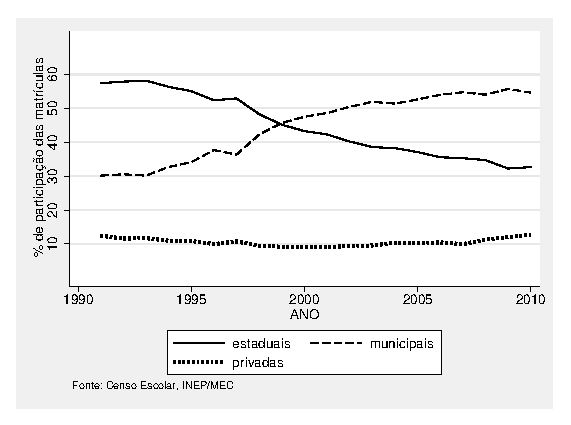
\includegraphics[height=3in]{share_matriculas}
\end{footnotesize}
\end{figure}
 
\vspace*{1cm} 


No primeiro grupo de trabalhos, h‡ uma profus‹o de trabalhos te—ricos e estudos de casos.\footnote{A esse respeito ver, entre outros, Gil e Arelano \citeyear{gil_contra_2004};  Araœjo \citeyear{araujo_municipio_2005}; Oliveira \citeyear{oliveira_municipalizacao_1999}; Pinto \citeyear{pinto_os_2000}}. Essa literatura, embora muito rica em estudos espec’ficos, Ž bastante limitada no exame sistem‡tico dos efeitos da descentraliazc‹o. Esses estudos, em geral, posicionam-se contra ou a favor da descentraliza‹o. 

Os defensores da descentraliza‹o argumentam que a transferncia de gastos e de poder de decis‹o para as esferas subnacionais pode tornar os governos mais responsivos ˆs preferncias dos cidad‹os Òadequando o provimento dos servios pœblicos a grupos menores e mais homogneosÓ \cite{wallis_impact_1998}. Essa argumenta‹o, que possui diferentes formula›es,\footnote{Essas formula›es v‹o desde a Òcompeti‹o predat—riaÓ de Paul Peterson \citeyear{peterson_price_1995} atŽ o Òfederalismo protetor do mercadoÓ de Bary Weingast \citeyear{weingast_economic_1995} passando pelas an‡lises de James Buchanan \citeyear{buchanan_federalism_1995} dentro da tradi‹o te—rica da public choice.} baseia-se nos trabalhos seminais de Charles Tiebout \citeyear{tiebout_pure_1956} e Wallace Oates \citeyear{oates_fiscal_1972} para quem a descentraliza‹o fiscal Ð e a conseqŸente competi‹o entre os governos locais Ð aparece como uma forma de mimetizar o mercado de bens privados para regular a oferta e a demanda de bens pœblicos\footnote{Entre os principais entusiastas da descentraliza‹o que se ap—iam nos argumentos de mais eficincia e democracia nas pol’ticas pœblicas ver, entre outros: Borja \citeyear{borja_descentralizacion_1987},  Borja et al \citeyear{borja_estado_1989}, Bennet \citeyear{bennett_decentralization_1990}, Olowu at al. \citeyear{olowu_local_2004} , Putnam \citeyear{putnam_making_1994} , UNDP \citeyear{united_human_1993} , World Bank \citeyear{world_world_1994}. Para uma cr’tica dessa linha argumentativa ver Arretche \citeyear{arretche_mitos_1996}.}.

Para os cr’ticos da descentraliza‹o, por outro lado, esta tende a contribuir para o fortalecimento das elites pol’ticas locais e de suas pr‡ticas clientel’sticas. Ademais, segundo a vers‹o cr’tica, os governos locais carecem dos recursos financeiros, tŽcnicos e humanos necess‡rios para um provimento eficiente das demandas locais\footnote{Para trabalhos com um enfoque mais cr’tico aos efeitos da descentraliza‹o ver: Murillo \citeyear{murillo_recovering_1999}, Kraemer \citeyear{kraemer_intergovernmental_1997}, Crook e Sverrisson \citeyear{crook_what_1999}, PrudÕhomme \citeyear{prudhomme_dangers_1995}, Samoff \citeyear{samoff_decentralization_1990} e Tanzi \citeyear{tanzi_fiscal_1996}, entre outros.}. Essa cr’tica, quando direcionada especificamente ao caso da educa‹o brasileira, enfatiza Ð alŽm dos fatores apontados acima Ð que a ausncia de coordena‹o entre os sistemas educacionais de estados e munic’pios no Brasil teria gerado uma mir’ade de propostas pedag—gicas e pol’ticas educacionais, n‹o apenas dispares entre si, mas em alguns casos, mesmo contradit—rias.

O Segundo grupo de an‡lises, que busca compreender as origens e causas da descentraliza‹o, Ž seguramente a maior, mais diversa e consolidada parcela da literatura em Cincia Pol’tica que trata da descentraliza‹o. Em geral, essa literatura explica a descentraliza‹o como uma fun‹o de: (i) incentivos eleitorais ou, (ii) de caracter’sticas do sistema partid‡rio. Riker \citeyear{riker_federalism:_1964}, por exemplo, argumenta que o grau de descentraliza‹o das federa›es depende, fundamentalmente, da estrutura de seus partidos pol’ticos. Ou seja, segundo Riker, a descentraliza‹o dos sistemas federativos est‡ diretamente relacionada ao grau de descentraliza‹o do sistema partid‡rio. Assim, se a descentraliza‹o dos Estados federativos est‡ associada ˆ estrutura do sistema partid‡rio, os processos de centraliza‹o e descentraliza‹o poderiam ser explicados em fun‹o das varia›es na estrutura dos sistemas partid‡rios e dos partidos pol’ticos. Mudanas nos partidos e nos sistemas partid‡rios seriam seguidas de altera›es no grau de centraliza‹o ou descentraliza‹o das federa›es.

J‡ para Kathleen OÕNeill \citeyear{oneill_decentralization_2003}, por outro lado, a gnese dos processos de descentraliza‹o est‡ mormente relacionada ao calculo eleitoral dos partidos pol’ticos. A descentraliza‹o afigura-se, assim para a autora, uma estratŽgia eleitoral de partidos que tm maiores chances de vit—ria em elei›es subnacionais. Segundo OÕNeill, a ado‹o de elei›es diretas para governadores e prefeitos foi o principal motivo para a descentraliza‹o pol’tica na Bol’via, Equador, Peru, e Col™mbia.

Merilee Grindle \citeyear{grindle_despite_2004} trata, mais especificamente, do caso da descentraliza‹o do sistemas educacionais de alguns pa’ses da America Latina. Grindle baseia sua an‡lise no c‡lculo estratŽgico dos atores envolvidos nas pol’ticas de reforma e descentraliza‹o; principalmente, dos partidos pol’ticos. A autora enfatiza o papel decisivo da ado‹o de elei›es diretas para os governos locais na Argentina, na Bol’via e na Venezuela nos processos de democratiza‹o e de descentraliza‹o pol’tica nesses trs pa’ses. Grindle pergunta-se, por que pol’ticos racionais abririam m‹o do poder em benef’cio de esferas subnacionais? Para concluir: a cria‹o de novas institui›es pol’ticas, e a descentraliza‹o em particular, precisa ser entendida em uma perspectiva te—rica que v‡ alŽm dos ganhos imediatos dos atores. Segundo a autora, empiricamente as motiva›es dos partidos e das elites pol’ticas s‹o complexas, n‹o se limitam a seus interesses imediatos, mas tambŽm reverberam conflitos mais persistentes de suas sociedades.

Willis, Garman e Haggard \citeyear{willis_politics_1999} e Garman, Haggard e Willis \citeyear{garman_fiscal_2001} apresentam duas an‡lises recentes a respeito da descentraliza‹o fiscal na AmŽrica Latina. Para os autores, a descentraliza‹o Ð e o grau em que esta ocorre Ð correlaciona-se ao n’vel de dependncia e reciprocidade entre os candidatos dentro dos partidos pol’ticos nacionais. Ou seja, Òquanto maior a sensibilidade pol’tica dos governantes na esfera central aos resultados eleitorais nos n’veis subnacionais, mais alta a probabilidade do sistema fiscal ser mais descentralizadoÓ (1999: 9). 

Os trabalhos de Willis, Garman e Haggard, como tambŽm a an‡lise de Kent Eaton \citeyear{eaton_decentralization_2000} sobre as reformas fiscais na Argentina e nas Filipinas, chamam aten‹o para as rela›es de dependncia, reciprocidade e lealdade entre o executivo nacional e os representantes locais no legislativo nacional. Os autores argumentam que a medida em que os legisladores argentinos dependem do executivo nacional para se manter no poder (devido ˆs regras eleitorais que estabelecem um sistema de lista fechada e representa‹o proporcional, no qual a indica‹o e a ordem dos candidatos dependem da burocracia partid‡ria nacional) suas preferncias sobre descentraliza‹o fiscal s‹o frequentemente mais pr—ximas das preferncias do presidente do que das preferncias dos governadores. Portanto, os legisladores s‹o muitas vezes relutantes em descentralizar gastos e receitas em benef’cio das esferas subnacionais de governo.

Ainda dentro dessa tradi‹o de analise das causas e origens da descentraliza‹o; porŽm, mais especificamente relacionado aos objetivos do presente trabalho, cabe destacar o estudo de Sandra Gomes (2008). Gomes (2008) analisa o processo recente de municipaliza‹o da educa‹o fundamental no Brasil. A autora contesta a interpreta‹o dominante de que as mudanas nas regras de financiamento da educa‹o trazidas pelo FUNDEF seriam um fator suficiente para explicar a municipaliza‹o da educa‹o fundamental no Brasil. Essa interpreta‹o, prevalente na literatura econ™mica brasileira, decorre de associa‹o autom‡tica entre a implementa‹o do FUNDEF e um aumento significativo da municipaliza‹o do ensino fundamental no Brasil. A municipaliza‹o, segundo Gomes, s— pode ser explicada por um conjunto mais amplo de fatores que incluem outras regras federais e estaduais. Tais como, a situa‹o das contas pœblicas no momento da implementa‹o do FUNDEF, o patamar inicial das matr’culas, o partido pol’tico de governadores e prefeitos e outras vari‡veis de contexto local, como disponibilidade orament‡ria e aspectos demogr‡ficos.

Em suma, a produ‹o acadmica na ‡rea de cincia pol’tica que procura investigar as causas, as caracter’sticas e os efeitos da descentraliza‹o tende a destacar o protagonismo do sistema eleitoral, dos partidos pol’ticos e do sistema partid‡rio, mas parecem negligenciar as conseqŸncias Ð e os resultados Ð da pol’tica de descentraliza‹o. E, mais importante, esses trabalhos sobre a descentraliza‹o explicam quase exclusivamente o n’vel de descentraliza‹o fiscal Ð medido como parcela dos gastos executados e receitas coletadas pelos governos subnacionais Ð, n‹o h‡ de fato muitos trabalhos devotados ˆ an‡lise da descentraliza‹o dos servios pœblicos, tais como saœde, educa‹o, assistncia social de uma perspectiva da cincia pol’tica\footnote{AlŽm dos j‡ mencionados trabalhos de Arretche \citeyear{arretche_estado_2000} e Falleti \citeyear{falleti_sequential_2005}, outra exce‹o digna de nota Ž: Ward e Rodrigues \citeyear{ward_new_1999}.}, apesar do peso dessas ‡reas na composi‹o dos gastos pœblicos.

Finalmente, nota-se na literatura um terceiro grupo de analises, predominantemente econ™micas, que buscam examinar os resultados da descentraliza‹o em termos de seus impactos para a qualidade e eficincia da provis‹o dos servios pœblicos. Na literatura econ™mica h‡ tradi›es espec’ficas em diferentes ‡reas que abordam o problema da provis‹o descentralizada de servios pœblicos. De tal sorte que, por exemplo, a economia da saœde, a economia da educa‹o e a economia urbana produziram importantes trabalhos que tratam dessa quest‹o. O presente trabalho p›e em evidncia apenas os estudos que examinaram a descentraliza‹o em educa‹o.

Nesse grupo de estudos encontram-se, sobretudo, trabalhos emp’ricos que Ð por meio de tŽcnicas economŽtricas Ð procuram avaliar o impacto de fatores variados no desempenho dos estudantes. Assim, estes estudos buscam, sistematicamente, mensurar o efeito de fatores como, por exemplo, recursos familiares, recursos escolares, custos de oportunidade da educa‹o, e o sistema educacional ao qual a escola se vincula (particular, pœblico estadual ou pœblico municipal) tm sobre o desempenho dos estudantes ou das escolas.

Como j‡ observado, se por um lado os trabalhos te—ricos oferecem respostas amb’guas (e mesmo contradit—rias) quanto aos efeitos da descentraliza‹o na provis‹o da educa‹o pelo setor pœblico; por outro lado, as evidncias emp’ricas reunidas atŽ o momento tampouco s‹o conclusivas. Segundo uma revis‹o de Faguet e S‡nchez \citeyear{faguet_decentralizations_2008}, de 24 artigos que apareceram na publica‹o ÒWorld DevelopmentÓ sobre descentraliza‹o, governos locais e responsabiliza‹o (i.e. accountability) desde 1997, 11 posicionaram-se favoravelmente aos resultados atingidos pelos programas de descentraliza‹o e 13 reportaram resultados negativos.

O trabalho de Faguet e Sanchez Ž firmemente favor‡vel aos resultados do processo de descentraliza‹o da educa‹o na Bol’via e na Col™mbia. As evidncias emp’ricas levantadas nesse estudo parecem indicar que a descentraliza‹o alterou os padr›es dos investimentos pœblicos nesses dois pa’ses tornando-os mais responsivos ˆs demandas das classes populares. Recursos que antes eram majoritariamente destinados a infra-estrutura e indœstria local passaram a se concentrar em ‡reas sociais, tais como: educa‹o, saœde e saneamento b‡sico.

Burki, Perry e Dillinger \citeyear{burki_beyond_1999}, em sua an‡lise da descentraliza‹o da educa‹o para um grupo de pa’ses da AmŽrica Latina, sugerem que a transferncia da responsabilidade pela provis‹o de educa‹o prim‡ria para os governos locais parece n‹o ter sido suficiente para que os resultados (positivos) esperados fossem atingidos. Segundo argumentam, a transferncia de autoridade e atribui›es deve ser feita diretamente ˆs unidades escolares e aos conselhos de pais e mestres para que as conseqŸncias positivas da descentraliza‹o surtam efeito. A simples transferncia da execu‹o dos gastos para os governos locais e regionais, como nos casos de Col™mbia e MŽxico, raramente viabiliza por si s— a melhoria dos resultados escolares. Em contraste, esforos para transferir ˆ gest‹o do ensino diretamente aos conselhos comunit‡rios ou ˆs unidades escolares como se deu em alguns casos analisados pelos autores, em pa’ses t‹o diversos como a Nicar‡gua, El Salvador, e Minas Gerais no Brasil, parecem apresentar resultados mais positivos.

O estudo de Filmer e Eskeland \citeyear{filmer_autonomy_2002} sobre a Argentina, onde a transferncia deu-se do governo central para os governos das prov’ncias, vale-se de um modelo econ™mico de fun‹o de produ‹o para examinar o impacto de programas de autonomia escolar e de pol’ticas de incentivo da participa‹o de pais de alunos na gest‹o das escolas em testes de aprendizado dos estudantes. Sua an‡lise utiliza dados em corte temporal (\emph{cross-section}) de testes de aprendizado em matem‡tica e espanhol e um ’ndice de autonomia escolar e participa‹o dos pais. A constru‹o desse ’ndice Ž feita por meio de vinte e oito vari‡veis que buscam mensurar o grau de autonomia escolar com base nas decis›es acerca de gest‹o de pessoal, organiza‹o do ensino e o grau de participa‹o dos pais de alunos nessas mesmas decis›es. Seus resultados s‹o amb’guos. Apontam que a autonomia escolar e a participa‹o dos pais est‹o positivamente relacionadas com o aprendizado em matem‡tica, porŽm n‹o com espanhol. Ademais, esses resultados apresentam maior signific‰ncia estat’stica para as escolas situadas nos bairros mais pobres e para os alunos oriundos dos segmentos menos favorecidos economicamente.

Entretanto, a maior deficincia do estudo de Filmer e Eskeland parece ser um poss’vel viŽs em seus resultados devido ˆ endogeneidade entre autonomia, participa‹o e vari‡veis n‹o observadas. Apesar da riqueza de seu banco de dados Ð que contŽm mais de vinte e quatro mil (24.000) observa›es para os testes de aprendizado dos estudantes de 6a e 7a sŽries Ð, a ausncia de informa›es mais precisas sobre autonomia escolar e participa‹o dos pais forou os autores a valer-se de vari‡veis instrumentais fracas. Por exemplo, eles descartam algumas vari‡veis explicativas importantes de seu modelo de fun‹o de produ‹o e as incluem como simples instrumentos (Filmer e Eskland, 2002: 20). Seus resultados, no entanto, s‹o relevantes, pois indicam que os benef’cios esperados da descentraliza‹o (do n’vel central para os governos locais ou regionais) podem ser potencializados se esta Ž capaz de criar incentivos ˆ autonomia escolar e ˆ participa‹o dos pais de alunos na gest‹o das escolas.

No Brasil, h‡ uma vasta literatura emp’rica\footnote{Os trabalhos emp’ricos em economia da educa‹o produzidos no Brasil s‹o, usualmente, classificados de acordo com a tem‡tica desenvolvida. De sorte que, h‡ um primeiro grupo de estudos que trata da mobilidade social e econ™mica em termos educacionais (Barros e Lam, \citeyear{de_barros_income_1993}; Ferreira e Veloso, \citeyear{ferreira_mobilidade_2003}; Marteleto, \citeyear{marteleto_desigualdade_2004}). Uma segunda linha de pesquisa que aborda a rela‹o de desigualdade de oportunidades e desigualdade de renda (Bourguignon et al. \citeyear{bourguignon_inequality_2003}; Menezes-Filho \citeyear{menezes-filho_educacao_2001}). J‡ a terceira vertente investiga a rela‹o entre trabalho infantil, pobreza e escolaridade (Emerson e Souza \citeyear{emerson_is_2003}\citeyear{emerson_child_2007}\citeyear{emerson_is_2011}; Kassouf \citeyear{kassouf_early_2001}; Barros et al.\citeyear{de_barros_os_1995}; Fernandes e Menezes-Filho \cite{fernandes_evolucao_2000}). No presente trabalho,  n‹o se faz uma resenha exaustiva dessa literatura. Ao contr‡rio, optou-se t‹o-somente por destacar aqueles trabalhos (independentemente da abordagem adotada) que dialogam direta ou indiretamente com a quest‹o da descentraliza‹o, mais especificamente, ou com a gest‹o escolar, mais amplamente.} sobre as rela›es existentes entre desempenho educacional de jovens e crianas e aspectos familiares como instru‹o dos pais e n’vel de renda da fam’lia; aspectos escolares como forma‹o dos professores e infra-estrutura f’sica das escolas e aspectos comunit‡rios como renda mŽdia da localidade ou o numero de escolas no munic’pio. Dentre os estudos emp’ricos, o trabalho seminal de Ricardo Paes de Barros e colaboradores (2001) Ž, seguramente, um dos mais importantes. Valendo-se de dados da Pesquisa Nacional por Amostra de Domic’lios (PNAD) e da Pesquisa de Padr›es de Vida (PPV), os autores indicam que, mesmo em se controlando por fatores como: recursos familiares, recursos escolares, custos de oportunidade da educa‹o, e o sistema educacional ao qual a escola se vincula (particular, pœblico estadual ou pœblico municipal), a escolaridade do indiv’duo (isto Ž, o nœmero de sŽries completadas) Ž mais diretamente afetada pela escolaridade dos pais e pela renda per capita da fam’lia. Os Recursos da comunidade (mensurados por meio da escolaridade mŽdia e da renda mŽdia dos moradores da localidade) e os recursos das escolas (mensurados pelo nœmero de escolas e pelo tempo mŽdio do trajeto atŽ a escola) apresentam um impacto positivo, porŽm estatisticamente n‹o significante. O n’vel de instru‹o dos professores apresenta um resultado amb’guo. Mostra-se positivo para as escolas de ensino fundamental e negativo para as escolas de ensino mŽdio (Barros et al., 2001).

O estudo de Albernaz, Ferreira e Franco \citeyear{albernaz_qualidade_2002} traz algumas importantes contribui›es nesse campo. AlŽm dos fatores analisados por Barros (2001), os autores incluem, com base em informa›es do SAEB de 1999,  outras vari‡veis sobre as escolas, como a qualidade da infra-estrutura f’sica e dados sobre forma‹o e experincia dos professores. A estima‹o proposta por Albernaz sugere que cerca de 80\% da vari‰ncia de desempenho mŽdio entre as escolas deve-se a diferenas na composi‹o socioecon™mica de seus alunos, refletindo um importante efeito de estratifica‹o socioecon™mica das escolas. Segundo, controlado esse efeito de estratifica‹o, o desempenho dos alunos est‡ significativamente relacionado com diferenas na qualidade e na quantidade de insumos escolares. Ao contr‡rio de resultados encontrados em estudos realizados em v‡rios outros pa’ses, tanto a qualidade dos professores como a qualidade da infra-estrutura f’sica das escolas afetam o rendimento de forma significativa\footnote{A relev‰ncia das vari‡veis escolares tem sido uma caracter’stica polmica, mas persistente, da literatura internacional sobre os fatores determinantes dos resultados educacionais. De acordo com a Tabela 3.23.1, p. 303 do Relat—rio Coleman \citeyear{coleman_equality_1966}, menos de 2 por cento da vari‰ncia total do desempenho dos alunos (brancos e negros) s‹o atribu’dos a caracter’sticas escolares, enquanto menos de 4 por cento s‹o atribu’dos a caracter’sticas dos professores. Em uma revis‹o mais recente dos estudos emp’ricos, Hanushek \citeyear{hanushek_expenditures_1989} apresenta um resumo das estimativas dos coeficientes dos gastos escolares sobre o desempenho dos alunos em 187 trabalhos da literatura internacional, chegando ˆ conclus‹o de que a œnica vari‡vel cuja relev‰ncia para o aprendizado dos alunos parece ser realmente robusta Ž a experincia do professor.}. Ademais, mesmo controlando por todos esses fatores, alunos de escolas particulares tm um desempenho mŽdio significativamente superior a de seus pares nas escolas publicas municipais ou estaduais.

Apesar do impacto muito elevado dos recursos familiares, os fatores relacionados a escola e a comunidade tambŽm apresentam um efeito n‹o desprez’vel no resultado educacional do indiv’duo. O estudo de Riani e Rios-Neto \citeyear{riani_background_2008} traz evidncias emp’ricas eloqŸentes que demonstram atŽ que ponto os fatores do perfil escolar do munic’pio podem minimizar a import‰ncia do ambiente familiar. Os resultados do trabalho de Riani indicam que aspectos relacionados a rede escolar dos munic’pios, principalmente, os de qualidade dos recursos humanos (tais como, instru‹o e experincia dos professores) e a infra-estrutura dos servios educacionais aumentam a probabilidade mŽdia do aluno freqŸentar a escola na idade correta.

Todos esses trabalhos contribu’ram para uma melhor compreens‹o do impacto de fatores associados aos recursos das fam’lias, das escolas e das comunidades nos resultados educacionais dos indiv’duos no Brasil. Entretanto, as vari‡veis relacionadas ˆs redes escolares ou ao n’vel de governo s‹o empregadas nesses estudos t‹o-somente como vari‡veis de controle. Particularmente, as vari‡veis associadas ˆ gest‹o dos sistemas educacionais e ˆ governana das escolas s‹o raramente tratadas como aspectos centrais da an‡lise desses estudos.\footnote{O acumulo de evidncias emp’ricas de que as escolas est‹o longe de verter mais recursos em melhores resultados educacionais (e.g. Hanushek, \citeyear{hanushek_interpreting_1995} \citeyear{hanushek_education_1994} ), levou a um interesse crescente de quest›es relacionadas ˆ gest‹o dos sistemas de ensino e ˆ governana das escolas. Dentro desse contexto a quest‹o da descentraliza‹o da educa‹o tem merecido um lugar de destaque na agenda de pesquisadores e decisores pol’ticos.} Nesse sentido, os trabalhos de DÕAtri \citeyear{datri_municipalizacao_2007}, Madeira \citeyear{madeira_effect_2007}, Leme e colaboradores \citeyear{leme_municipalizacao_2009} e Orellano e colaboradores \citeyear{orellano_descentralizacao_2010} trazem contribui›es relevantes ao examinar diretamente o impacto da descentraliza‹o das escolas nos resultados do ensino pœblico no Brasil. 

O estudo de DÕAtri (2007) utiliza dados do Censo Escolar do MEC/INEP para avaliar o impacto da municipaliza‹o das escolas nas taxas de matricula, taxas de abandono e na distor‹o idade-sŽrie dos alunos. Controlando por caracter’sticas das escolas e dos alunos, DÕAtri compara os dados do Censo Escolar de 1998 e 2004. Seus principais resultados indicam que as escolas municipais apresentam desempenho pior do que as escolas estaduais para as vari‡veis acima mencionadas. Mais importante, o estudo de DÕAtri aponta que os resultados inferiores da escolas municipais devem ser atribu’dos mais diretamente a r‡pida expans‹o dos sistemas municipais de ensino do que a transferncia de controle de escolas dos estados para os munic’pios.

A an‡lise de Madeira (2007) restringe-se ˆs escolas do estado de S‹o Paulo, que vem conduzindo um consider‡vel esforo de municipaliza‹o das matriculas. Madeira procura mensurar o impacto da transferncia de controle do ensino fundamental sobre as taxas de matricula, taxas de abandono e distor‹o idade-sŽrie. AlŽm disso, busca avaliar o impacto da municipaliza‹o sobre a de utiliza‹o de alguns insumos escolares, tais como: numero de horas em sala de aula, tamanho das turmas, e utiliza‹o de equipamentos e infra-estrutura f’sica das escolas. Para tanto, serve-se dos dados do Censo Escolar de 1996 a 2003. Seus resultados apontam que, se por um lado, verifica-se um impacto positivo na utiliza‹o dos insumos escolares (horas-aula, tamanho das turmas, etc.). Por outro lado, verifica-se um impacto negativo nas taxas de matricula, taxas de abandono e distor‹o idade-sŽrie. Vale lambrar que, seus resultados confirmam o trabalho de DÕAtri (2007).

A investiga‹o de Orellano e colaboradores (2010) tambŽm vale-se de dados do Censo Escolar do MEC/INEP para estimar os efeitos do aumento das matr’culas e dos gastos municipais em educa‹o fundamental sobre  trs indicadores de rendimento do fluxo escolar, as taxas de aprova‹o, abandono escolar e a distor‹o idade-sŽrie. A principal contribui‹o desse estudo Ž incorporar tanto aspectos relativos ˆ autonomia municipal de arrecada‹o e de gastos, quanto aqueles relacionados ˆ gest‹o municipal das escolas, o que possibilita aos autores examinar o efeito independente tanto da municipaliza‹o das matr’culas como da descentraliza‹o fiscal sobre os produtos educacionais dos munic’pios. A despeito de algumas limita›es emp’ricas n‹o desprez’veis, o estudo apresenta uma forte associa‹o positiva entre descentraliza‹o fiscal e desempenho em educa‹o, resultado este que n‹o se repete para o n’vel de municipaliza‹o das matr’culas. Ou seja, segundo Orellano, quando maior o n’vel de descentraliza‹o fiscal mais altas as taxas de matr’cula e menores as taxas de abandono escolar. PorŽm, quando se considera o n’vel de municipaliza‹o das matr’culas como medida de descentraliza‹o essa associa‹o positiva desaparece. 

As contribui›es de DÕAtri (2007), Madeira (2007) e Orellano e colaboradores (2010) s‹o, sem dœvida, muito importantes; contudo, apresentam algumas limita›es. A principal delas refere-se ao uso exclusivo de indicadores de rendimento dos sistemas de ensino, tais como taxas de matriculas, aprova‹o ou abandono escolar, abdicando da utiliza‹o de indicadores de desempenho dos alunos. O emprego exclusivo de vari‡veis como taxa de matricula, taxa de abandono ou mesmo a taxa defasagem idade-sŽrie como indicadores educacionais pode conduzir a distor›es; pois, essas vari‡veis s‹o afetadas por fatores que n‹o se relacionam diretamente com a gest‹o da escola, com a fam’lia ou mesmo com a comunidade. Essas vari‡veis s‹o, na verdade, suscet’veis a fatores ex—genos (e n‹o observ‡veis) tais como programas de progress‹o continuada (isto Ž, aprova‹o autom‡tica) ou mesmo ˆ r‡pida expans‹o do ensino fundamental experimentada pelo Brasil ao longo dos œltimos 20 anos. Outra limita‹o, particularmente dos estudos de DÕAtri e Orellano, diz respeito ao n’vel de agrega‹o. Ao servir-se t‹o-somente de dados para os munic’pios, esses estudos deixam de controlar os efeitos fixos das escolas, o que pode enviesar suas an‡lises.

O estudo de Orellano e colaboradores (2010), em particular, parece sofrer de um problema de endogeneidade entre o indicador de descentraliza‹o fiscal proposto pelos autores e os indicadores educacionais examinados, que pode estar enviesando as estimativas. Orellano vale-se da raz‹o entre as transferncias do FUNDEF recebidas pelos munic’pios e os gastos totais dos munic’pios em educa‹o como medida de descentraliza‹o fiscal. Contudo, essas medidas parecem ser end—genas, mesmo com o controle dos efeitos espec’fico dos munic’pios usado pelos autores. ƒ razo‡vel supor, por exemplo, que os prefeitos elevem seus gastos em educa‹o, afetando o comportamento da raz‹o FUNDEF/gastos, quando confrontados com maus resultados educacionais em seus munic’pios. Como se assume que essa medida de descentraliza‹o fiscal Ž exogena aos resultados educacionais, as estimativas apresentadas pelos autores podem estar sendo enviesadas por esse problema de endogeneidade dos regressores.

Ademais, h‡ um problema conceitual no trabalho de Orellano e colaboradores. Os autores tratam como equivalentes as transferncias do FUNDEF recebidas pelos munic’pios e a dependncia de transferncias do governo central. As transferncias do FUNDEF para os munic’pios n‹o est‡ vinculada a gera‹o de receitas fiscais pr—prias dos munic’pios. Mas, depende exclusivamente do nœmero de matr’culas no ensino fundamental em escolas publicas das redes municipais. Pois, a transferencia d‡-se em fun‹o de um valor fixo por aluno matriculado na rede pœblica. Ainda, as transferncias do FUNDEF n‹o s‹o compostas por recursos do governo central. Mas, sim, por recursos dos pr—prios estados e munic’pios. Salvo, um complemento federal, caso as transferncias do FUNDEF n‹o atinjam o piso nacional de gasto por aluno. H‡, portanto, no estudo de Orellano e colaboradores uma confus‹o entre transferncias do FUNDEF e dependncia do governo central. 

O estudo de Leme, Paredes e Souza \citeyear{leme_municipalizacao_2009} procura estimar o efeito da municipaliza‹o na proficincia dos alunos. Para tanto, serve-se do nœmero de escolas que passaram da gest‹o estadual para a gest‹o municipal como medida de descentraliza‹o e das avalia›es em matem‡tica e em l’ngua portuguesa no MEC/INEP  como medida de desempenho educacional. Segundo Leme e colaboradores, a municipaliza‹o das escolas parece n‹o ter tido nenhum efeito (positivo ou negativo) relevante no desempenho dos alunos de 4a. sŽrie do ensino fundamental. A ausncia de efeito not‡vel da municipaliza‹o no trabalho de Leme, Paredes e Souza parece decorrer tanto da amostra muito restrita com que trabalham os autores \footnote{Leme, Paredes e Souza (2010) identificam apenas 122 escolas que migraram do controle estadual para o controle municipal e que aparecem pelo menos duas vezes nas avalia›es do MEC/INEP entre os anos de 1999 e 2005.}, como tambŽm e, principalmente, pode ser que as vari‡veis de controle dos alunos e de suas fam’lias e o modelo de efeitos espec’ficos das escolas empregados pelos autores ainda n‹o apresentem a acuidade necess‡ria para se captar o efeito independente da municipaliza‹o das escolas sobre a proficincia dos alunos, como, ali‡s, admitem os pr—prios autores do trabalho. 

Em suma, embora a produ‹o acadmica esteja em franco processo de expans‹o e de acumulo de evidncias, a revis‹o dos trabalhos produzidos acerca da descentraliza‹o e do provimento de servios pœblicos (particularmente, da provis‹o pœblica de educa‹o fundamental no Brasil) sugerem n‹o apenas falta de consenso a respeito de seus efeitos como tambŽm parece indicar que as evidncias emp’ricas reunidas atŽ o presente momento s‹o inconclusivas.

O presente trabalho pretende contribuir com essa literatura investigando, inicialmente, se o n’vel de governo (e, consequentemente, a rede escolar) importa para o desempenho dos alunos. Em segundo lugar, a estratŽgia emp’rica proposta pela tese permiti contornar algumas das limita›es apontadas nos trabalhos anteriores.

A estratŽgia emp’rica proposta consiste em combinar an‡lises distintas de estima‹o dos efeitos da municipaliza‹o sobre (i) os alunos, (ii) as escolas, e (iii) os insumos e as taxas de rendimento do fluxo escolar nos munic’pios. Primeiro, servindo-se de um painel de escolas, com dados desagregados ao n’vel dos alunos, constru’do com base no SAEB para os anos entre 1997-2005 Ž estimada a diferena de desempenho dos alunos de escolas pœblicas municipais e escolas pœblicas estaduais. Essa estima‹o Ž feita com base nas usuais tŽcnicas de M’nimos Quadrados Ordin‡rios, Efeitos Aleat—rios e Efeitos Fixos, assegurando-se que os resultados s‹o robustos a diferentes modelos estat’sticos. Segundo, utilizando-se dados do SAEB e da Prova Brasil s‹o acompanhados (retrospectivamente) trs grupos de escolas em dois pontos no tempo: antes e depois da municipaliza‹o. Ou seja, Ž selecionado um grupo experimental de escolas que estavam sob controle estadual e foram transferidas para o controle municipal, e dois grupos controle de escolas que estavam sob a gest‹o estadual ou municipal e assim permaneceram. Dessa forma, Ž comparado, por meio de um modelo de estima‹o por diferena-em-diferenas, o efeito da municipaliza‹o das escolas sobre desempenho dos estudantes. Finalmente, Ž utilizado um painel de dados de 2837 munic’pios com informa›es do Censo Escolar e dos munic’pios entre os anos 1999 e 2005 para se estimar o efeito da municipaliza‹o das matr’culas e sobre uma sŽrie de indicadores de insumos educacionais e rendimento escolar nos munic’pios.

\pagebreak

\section{Definindo e Medindo Resultados Educacionais}

A avalia‹o educacional est‡ no centro do debate sobre educa‹o no Brasil e no exterior. Sua import‰ncia e seu impacto, seja no debate acadmico seja nas pr‡ticas dos formuladores pol’ticos, dificilmente passa despercebida a uma r‡pida folheada das gazetas di‡rias ou artigos dos peri—dicos especializados. Termos como: exames, instrumentos de avalia‹o, teoria da resposta ao item e outros oriundos do jarg‹o da ‡rea parecem ter ganhado o cotidiano de professores, estudantes, suas fam’lias e de cidad‹os informados. 

A extensa produ‹o acadmica acerca do tema Ð tanto na tradi‹o anglo-sax™nica quanto, mais recentemente, na literatura de l’ngua portuguesa Ð Ž uma constata‹o de sua import‰ncia. Entretanto, uma r‡pida revis‹o dos trabalhos produzidos no Brasil ou alhures revela que a defini‹o dos conceitos ainda carece de consenso quanto a seu significado e de clara delimita‹o te—rica. Percebe-se que a defini‹o tende a variar acentuadamente n‹o apenas de autor para autor, mas tambŽm conforme a tradi‹o disciplinar na qual o trabalho se insere.

Mais especificamente, os termos da lingua inglesa: \emph{assessment, evaluation, testing e measurement} s‹o muitas vezes usados como sin™nimos, como termos intercambi‡veis, ou mesmo definidos um tanto tautologicamente por meio de referncias reciprocas, como observou com precis‹o John Keeves \citeyear{keeves_educational_1997}. Na verdade, o que \emph{assessment, evaluation e measurement} tm em comum Ž que todos s‹o auferidos ou operacionalizados por meio de exames, ou testes. Isto Ž, \emph{assessment, evaluation e measurement} s‹o atividades que frequentemente, porŽm n‹o sempre, se valem de exames \footnote{No ambito desse trabalho os termos teste e exame s‹o utilizados como sin™nimos por quest›es meramente estil’sticas}. No entanto, vale ressaltar, que nenhuma dessas atividades limita-se ˆ simples aplica‹o de exames ou mesmo podem ser empregadas como sin™nimos desse œltimo. Principalmente, os tipos de exames empregados em cada uma dessas atividades Ž bastante diferente \cite{weiss_evaluation_1988}. A seguir s‹o oferecidas breves defini›es dos termos bem como uma descri‹o dos processos que comp›em cada uma dessas atividades educacionais. Numa segunda etapa, define-se operacionalmente o que se entende, no ‰mbito desse trabalho, por resultados educacionais. Ent‹o, Ž apresentado o SAEB e um brev’ssimo sum‡rio de seus principais resultados.

   
\subsection{Mensura‹o}	

Segundo o dicion‡rio Houaiss da L’ngua Portuguesa, a defini‹o de mensura‹o Ž "medir, determinar as medidas de".  Tal defini‹o poderia ser empregada ˆ grande maioria das aplica›es de mensura‹o educacional sem preju’zos sem‰nticos. Nesse sentido, mensura‹o educacional refere-se ao conjunto de processos destinados e determinar as medidas de desempenho escolar, aprendizado, avalia‹o de conhecimentos e avalia‹o de competncias, etc. Entretanto, Ž importante observar que enquanto instrumentos como cron™metros e fita mŽtricas podem ser utilizados para se determinar medias de velocidade e comprimento quase diretamente; a grande maioria das medidas de interesse educacional s‹o mensuradas apenas incompleta e indiretamente. Mais precisamente, as medidas de desempenho educacional obtidas por meio de testes de avalia‹o s‹o \emph{proxys} de uma conjunto mais abrangente de conhecimentos e competncias que n‹o podem ser diretamente auferidos \cite{koretz_measuring_2008}. 

No dia 30 de outubro de 2010 (`as vŽsperas das elei›es gerais), o IBOPE divulgou uma pesquisa de opini‹o eleitoral para a presidncia da Republica com os resultados de uma amostra de 3010 eleitores. As estimativas mostravam a candidata do PT, Dilma Rousseff, com 52 por cento das inten›es de voto e o candidato do PSDB, JosŽ Serra, com 40 por cento.  Os resultados finais das elei›es demostraram que a previs‹o do IBOPE estava razoavelmente correta. A diferena final foi de aproximadamente 12 por cento. A mensura‹o educacional Ž em muitos sentidos semelhante ˆs pesquisas eleitorais. 

O conjunto mais abrangente de habilidades e conhecimentos a respeito do qual os exames fornecem uma estimativa Ž usualmente denominado \emph{dom’nio}. O dom’nio seria o equivalente ˆ vota‹o de toda a popula‹o de eleitores na pesquisa do IBOPE. Assim como n‹o seria razo‡vel (ou mesmo exequ’vel) que os pesquisadores do IBOPE entrevistassem todo o eleitorado, tampouco seria razo‡vel que um teste de desempenho escolar fosse capaz mensurar exaustivamente o dom’nio de um aluno ou conjunto de alunos. Simplesmente, porque dom’nios s‹o, em geral, muito vastos e abrangentes para serem cobertos por um exame. Analogamente, assim como Ž poss’vel se estimar a inten‹o de voto do eleitorado de aproximadamente 130 milh›es de brasileiros a partir de uma amostra de pouco mais de 3000 poss’veis eleitores, Ž aplicado um teste de desempenho escolar que cobre t‹o-somente uma pequena amostra do dom’nio do aluno para se obter uma estimativa de sua compreens‹o sobre determinado assunto, disciplina acadmica ou competncia cognitiva.

De tal sorte que, tipicamente, exames de proficincia s‹o utilizados para se determinar medias de conhecimento sobre um determinado assunto, tema ou disciplina acadmica enquanto testes de habilidades ou competncias s‹o empregados para se determinar medidas de inteligncia ou para se obter um padr‹o de referncia em que se analisa nos alunos a capacidade de racioc’nio, o uso da l’ngua, a capacidade de express‹o e a de resolver determinados tipos de problemas \cite{keats_causal_1988}. Finalmente, Deve-se ressaltar que a mensura‹o educacional n‹o se trata de uma finalidade em si mesmo. Mas, ao contr‡rio, trata-se de uma atividade œtil no processo de se avaliar conhecimentos e competncias, ou como uma atividade de apoio ˆ avalia‹o escolar, etc. Assim, mensura‹o refere-se a todos os aspectos e processos de constru‹o de exames e testes educacionais.

\subsubsection{Mensura‹o no SAEB}

Ao contr‡rio de um exame cl‡ssico, como o que um professor aplica regularmente a seus alunos em sala de aula, os testes do SAEB e da Prova Brasil s‹o constru’dos metodologicamente para avaliar os sistemas de ensino, e n‹o alunos (MEC/INEP, 2005)\footnote{Como se comentar‡, mais pormenorizadamente, adiante a amostra do SAEB Ž representativa para os estados e as redes de ensino no Brasil}. A proficincia dos estudantes Ž mensurada em uma escala de desempenho concebida para descrever, em cada n’vel, as competncias e as habilidades que os estudantes desses sistemas demonstram ter desenvolvido ao longo de sua trajet—ria escolar. H‡ uma escala descrita para as habilidades em l’ngua portuguesa e outra para matem‡tica. A Tabela \ref{tab: tabsaeb}  descrve as habilidades e competncias correspondentes aos diferentes n’veis de proficincia em l’ngua portuguesa. Vale ressaltar que, dentro de cada uma das disciplinas, a escala Ž œnica e cumulativa, para todas as sŽries avaliadas. A l—gica subjacente a essa estratŽgia de mensura‹o Ž que quanto mais o estudante caminha ao longo da escala, mais habilidades ter‡ acumulado. Portanto, Ž esperado que alunos da 4» sŽrie do ensino fundamental\footnote{N‹o obstante n‹o exista um n’vel ideal de desempenho para os estudantes definido pelo MEC, o movimento \emph{Todos pela Educa‹o}, por exemplo, considera que um aluno de 4a. sŽrie do ensino fundamental alcance pelo menos 200 pontos em l’ngua portuguesa e 225 em matem‡tica na escala SAEB. Ver a esse respeito \url{http//:www.todospelaeducacao.org.br/}.} alcancem mŽdias numŽricas menores que os alunos de 8» sŽrie e estes alcancem mŽdias menores que as alcanadas pelos alunos de 3¼ ano do ensino mŽdio.


%%%%%%%%%%%%%%%%%%%%%%%%%%
%%%%%%%%%%%%%%%%%%%%%%%%%%


\begin{table}\centering
\begin{footnotesize}
\def\sym#1{\ifmmode^{#1}\else\(^{#1}\)\fi}
\caption{N’veis de Desempenho em L’ngua Portuguesa: escala œnica SAEB} 
\label{tab: tabsaeb}
\begin{tabular}{p{3cm} | p{9cm}}  
\toprule
\bf{Proficincia}   &  \bf{Competncia e habilidades}  \\
\midrule
\hline
Abaixo do N’vel 1 ($PROFIC < 150$) & N‹o atingiu as habilidades b‡sicas que o SAEB objetivava mensurar \\
\hline
N’vel 1 ($150 ³ PROFIC < 200$) &  Operar preferencialmente com estratŽgias locais de leitura. Identificar informa›es cruciais/centrais em posi‹o destacada. E a finalidade ou tema de um texto. Usar conhecimento de mundo na percep‹o do sentido de um texto. \\
\hline
N’vel 2 ($200 ³ PROFIC < 250$) & Resolver problemas de leitura a partir da compreens‹o global do texto, incluindo inferncias. Localizar informa›es secund‡rias. Reconstruir uma narrativa, encadeando v‡rios fatos na ordem de apari‹o. Reconhecer efeitos de sentido de recursos variados (repeti‹o, substitui‹o, onomatopŽia). \\
\hline
N’vel 3 ($250 ³ PROFIC < 300$) & Estabelecer rela›es coesivas entre partes do texto, inclusive pelo reconhecimento de t—pico e coment‡rio. Distinguir ÒfatoÓ de Òopini‹oÓ; problema de solu‹o; tese de argumento; causa de efeito. Fazer transforma›es estruturais e estabelecer rela›es de correspondncia. Compreender explica›es mais abstratas, metalingŸ’sticas.  \\
\hline
N’vel 4 ($300 ³ PROFIC < 350$) & Comparar textos afins, identificando e avaliando as estratŽgias argumentativas e a finalidade de cada um. Estabelecer rela›es sint‡tico/sem‰nticas na progress‹o tem‡tica. Mostrar conhecimento da estrutura e do funcionamento dos gneros textuais. Apresentar boa no‹o da rela‹o entre linguagem e sociedade. \\
\hline
N’vel 5 ($350 ³ PROFIC < 400$) & Trabalhar com linguagem figurada/conotativa em
n’vel global, articulado. Identificar diferentes n’veis de tratamento tem‡tico, reconhecendo t—picos e subt—picos. Analisar o efeito da sele‹o lexical em uma argumenta‹o. Aplicar com propriedade conhecimentos metalingu’sticos e liter‡rios.  \\
\hline
\bottomrule
\multicolumn{2}{l}{\footnotesize Fonte: MEC/INEP}\\
\end{tabular}
\end{footnotesize}
\end{table}

\vspace*{1cm} 

%%%%%%%%%%%%%%%%%%%%%%%%%%
%%%%%%%%%%%%%%%%%%%%%%%%%%




\subsection{Avalia‹o}

Em geral, o uso do termo avalia‹o educacional (\emph{educational evaluation}, na l’ngua inglesa) refere-se a avalia‹o de entidades coletivas ou abstratas; tais como, programas, curr’culos, situa›es organizacionais, escolas ou sistemas escolares, etc. Seu emprego envolve n‹o apenas a determina‹o da qualidade, da extens‹o ou da intensidade; mas implica tambŽm em estimar a valia, em estabelecer o merecimento.  ÒAvaliar Ž atribuir valorÓ lembra Brian Barry \citeyear{barry_political_1975}. A avalia‹o educacional, assim sendo, vale-se usualmente de compara›es com algum tipo de padr‹o te—rico, de objetivos previamente estabelecidos, de outros programas ou de outros curr’culos.

Nesse sentido, a avalia‹o educacional diferencia-se das atividades de auditagem financeira e de controle procedimental ligados ˆ administra‹o pœblica. As atividades consideradas aqui como relacionadas ˆ avalia‹o s‹o aquelas que buscam caracterizar a validade, utilidade, eficincia e efetividade de, por exemplo, curr’culos, programas pedag—gicos ou pol’ticas educacionais, em termos de seus resultados, impactos e repercuss›es econ™micas e sociais, e que, desse modo, tm como meta a gera‹o de resultados ou recomenda›es para o aprimoramento das pr‡ticas educacionais. Enfim, a avalia‹o de um objeto qualquer (como um curr’culo escolar, ou um programa de reforo escolar) Ž feita para identificar e aplicar critŽrios defens‡veis para determinar seu valor, mŽrito ou qualidade.

Essa compreens‹o do objetivo b‡sico da avalia‹o Ž hoje a mais aceita na literatura e adotada por organiza›es de peso que trabalham no campo da avalia‹o educacional, tendo sido incorporada ˆs ÒDiretrizes para a Avalia‹o de ProgramasÓ desenvolvidas pelo Comit Conjunto para Diretrizes da Avalia‹o Educacional \footnote{No original: \emph{The Program Evaluation Standards e Joint Committee on Standards for Education Evaluation}, tradu‹o do autor. O ÒComit Conjunto para Diretrizes da Avalia‹o EducacionalÓ Ž uma associa‹o profissional, com sede na Western Michigan University, que congrega pesquisadores e avaliadores e publica regularmente obras voltadas ˆ dissemina‹o de pesquisas e ˆ padroniza‹o das boas pr‡ticas no ‰mbito da avalia‹o educacional. As ÒDiretrizes para a Avalia‹o de ProgramasÓ encontram-se atualmente em sua 3a. edi‹o (Sage Publications, 2010). Uma vers‹o resumida dessas diretrizes pode ser consultada na p‡gina do —rg‹o na Internet em: \url{ www.jcsee.org/}} (2010). Embora essa vis‹o seja aceita por muitos, n‹o Ž consensual. Outros pesquisadores e avaliadores de prest’gio, como por exemplo Shadish  \citeyear{shadish_need-based_1994,shadish_experimental_2002}, Talmage \citeyear{talmage_evaluation_1982} e Fetterman  \citeyear{fetterman_empowerment_1994}, afirmam que a avalia‹o tem v‡rios objetivos. Talmage assinala que Òtrs objetivos parecem ser os mais freqŸentes nas defini›es de avalia‹o: fazer julgamentos de valor de um programa; ajudar os respons‡veis pela tomada de decis›es a definir suas pol’ticas; e, assumir uma fun‹o pol’ticaÓ (1982: 594). Talmage nota tambŽm que, ainda que esses objetivos n‹o sejam mutuamente exclusivos, s‹o claramente diferentes entre si.

Weiss \citeyear{weiss_how_1997} aponta que, de modo geral, os estudos e pesquisas de avalia‹o est‹o relacionados com os seguintes prop—sitos: informa‹o para o processo decis—rio, ou tomada de decis‹o, e aprendizado organizacional. Como lembra, com exatid‹o, S™nia Draibe \citeyear{draibe_avaliacao_2001}, s‹o objetivos dessa natureza que fazem da avalia‹o de educacional uma pesquisa interessada Ð ou, para conservar as palavras da autora, \emph{policy oriented} Ð, pois trata-se de uma atividade que busca identificar obst‡culos, propor medidas de corre‹o e altera‹o de pol’ticas e programas. Isto Ž, a avalia‹o n‹o constitui uma atividade neutra, imparcial ou impessoal, mas Ž uma atividade que, por sua pr—pria natureza, condi›es e mŽtodos, constitui-se numa a‹o interessada e, necessariamente, conflitiva. Pois, embora sua import‰ncia no aprimoramento das pr‡ticas educativas seja amplamente reconhecida, seus objetivos, usos e efeitos para estudantes, professores e escolas s‹o objeto de intenso debate e conflito pol’tico. 

Finalmente, cade observar que a avalia‹o educacional apoia-se metodologicamente na mensura‹o dos resultados educacionais. Para tanto, pode valer-se do uso de testes de desempenho escolar ou exames de habilidades de indiv’duos ou grupos. Assim, a avalia‹o educacional refere-se a todos os processos de coleta sistem‡tica de informa›es acerca de atividades, caracter’sticas, resultados e produtos para o uso espec’fico de tomada de decis›es a respeito da gest‹o de pol’ticas, programas e pr‡ticas educacionais. 

\subsection{Resultados Educacionais}

Desde meados dos anos 1990, os governos no Brasil vm realizando esforos para o aprimoramento da coleta de informa›es e produ‹o de estat’sticas acerca da provis‹o dos servios de educa‹o. Ademais, neste per’odo, assistiu-se a um movimento consistente de formaliza‹o e consolida‹o de programas de avalia‹o educacional, tanto por parte do MinistŽrio da Educa‹o (MEC), que promove desde 1990 aferi›es do Sistema de Avalia‹o da Educa‹o B‡sica (SAEB), como pelas Secretarias de Educa‹o dos estados e munic’pios  que desenvolvem iniciativas locais de avalia‹o de suas redes escolares. Esses programas locais assumem aspectos peculiares e se encontram em est‡gios diferentes de institucionaliza‹o nos diversos estados e munic’pios.\footnote{Bahia, Cear‡, Minas Gerais, S‹o Paulo, Paran‡, Pernambuco e Rio de Janeiro, entre outros, implataram e consolidaram sistemas de avalia‹o de suas redes escolares nos œltimos anos.}

Esses programas de avalia‹o das redes escolares inserem-se num quadro mais amplo de iniciativas que visavam reestruturar o papel do Estado, principalmente em rela‹o as suas fun›es e atua‹o no campo social. Este movimento de reformas, no campo educativo, possui dois grandes eixos: a descentraliza‹o da gest‹o das redes de ensino e a implanta‹o de sistemas de avalia‹o das redes escolares \cite{castro_como_2003}.
N‹o obstante tais tentativas, mensurar os resultados em educa‹o continua sendo uma tarefa que apresenta obst‡culos n‹o triviais. A provis‹o de educa‹o b‡sica pelo setor pœblico envolve uma sŽrie de atividades e processos governamentais bastante complexos. O objetivo b‡sico da educa‹o Ð definido amplamente Ð Ž preparar os cidad‹os (estudantes) para participa‹o da vida em sociedade e na economia por meio do mercado de trabalho. Os resultados do sistema educacional, por sua vez, s‹o afetados por um conjunto de fatores que v‹o bem alŽm do que se passa entre os muros das escolas e do resultado das pol’ticas educacionais. Caracter’sticas socioecon™micas da fam’lia, habilidades dos estudantes, bem como outras vari‡veis associadas a caracter’sticas pessoais e familiares dos alunos afetam significativamente seu desempenho escolar.

Na literatura os termos resultados, produtos e desempenho educacional s‹o definidos sem exatid‹o por meio de referncias rec’procas. Mais importante, s‹o comumente utilizados indistintamente para se referir a um mesmo conjunto de indicadores. Em geral, resultados educacionais referem-se aos indicadores de desempenho dos alunos ou das escolas, incluindo mensura›es dos resultados do aprendizado dos estudantes. Tais medidas de resultados em educa‹o s‹o, em geral, agrupadas em dois conjuntos de indicadores: medidas de volume de recursos (e.g. numero de alunos, fluxo de coortes, investimento por aluno, etc.) e medidas de qualidade (e.g. desempenho em testes de aprendizado padronizados) \cite{atkinson_measurement_2005-1}.

H‡ muitos tipos diferentes de indicadores de desempenho, entre os principais indicadores utilizados, pode-se citar: (i) indicadores da provis‹o de recursos financeiros; (ii) taxas de acesso ou participa‹o nos n’veis prŽ-escolar, elementar, secund‡rio, vocacional e terci‡rio; (iii) custos de provis‹o educacional em cada um desses n’veis; (iv) tamanho da turma e/ou taxas de alunos por professor; (v) n’vel de treinamento dos professores e participa‹o no desenvolvimento profissional interno; medidas de aproveitamento dos alunos em ‡reas chave do curr’culo em determinados n’veis de idade-sŽrie; (vi) medidas do aprendizado dos alunos atravŽs do tempo, e dos fatores que afetam as taxas de progresso; (vii) medidas de efic‡cia dos programas para alunos com necessidades especiais e oriundos de condi›es desfavor‡veis.\footnote{Os tipos a alcances dos indicadores de desempenho educacionais utilizados em diferentes pa’ses encontram-se bem ilustrados na p‡gina do programa da UNESCO ÒAvalia‹o do ano 2000 da Educa‹o para Todos (EFA) na Internet em: \url{http://www2.unesco.org/efa/wef/contryreports/contry.html}.}

Optou-se neste trabalho, pela utiliza‹o dos indicadores mais comumente empregados pela literatura especializada. Um primeiro conjunto de indicadores diz respeito aos insumos escolares. Isto Ž, os recursos das escolas, que podem afetar o aprendizado dos alunos: como, por exemplo, escolariza‹o dos professores, experincia dos professores, infraetrutura f’sica das escolas, dentre outros fatores que s‹o regularmente mensurados pelo MEC/INEP por meio do Censo Escolar da Educa‹o B‡sica. Neste trabalho, deu-se deu-se preferncia ao exame de: a forma‹o e experincia dos professores, e a infraestrutura f’sica das escolas. O segundo conjunto de indicadores referem-se ˆs taxas de rendimento do fluxo escolar, esse conjunto de indicadores procura auferir o acesso ˆ educa‹o por meio da taxa de matr’cula, e o fluxo dos estudantes por meio das taxas de evas‹o, repeti‹o, e principalmente, por meio da taxa de defasagem idade-sŽrie. Neste trabalho, decidiu-se pelo uso dos indicadores de produtos educacionais mais comumente empregados na literatura, a saber: as taxas de repeti‹o, evas‹o e a distor‹o idade-sŽrie. Finalmente, o desempenho dos estudantes Ž auferido por meio dos testes de proficincia em Matem‡tica e L’ngua Portuguesa conduzidos pelo MEC/INEP, particularmente, pelo SAEB. Assim, no escopo desse trabalho, resultados educacionais referem-se especificamente ao rendimento dos sistemas escolares no munic’pios em termos de acesso e fluxo dos estudantes e ao desempenho dos estudantes nos testes de proficincia.

O acesso da popula‹o ao sistema educativo de um determinado pa’s, regi‹o ou munic’pio Ž geralmente medido por meio da(s) taxa(s) de matr’cula. A taxa de alfabetiza‹o indica os resultados acumulados do sistemas de educa‹o prim‡ria e dos programas de alfabetiza‹o destinados a capacitar a popula‹o com as habilidades mais b‡sicas de leitura e escrita. Entretanto, as taxas de matr’culas nos munic’pios brasileiros se estabilizaram a partir dos anos 2000, quando se atingiu a universaliza‹o de matr’culas para crianas em idade escolar (6 a 14 anos de idade). Sua flutua‹o Ž hoje atribu’da, quase que exclusivamente, a fatores demogr‡ficos, principalmente ˆ taxa de natalidade (MEC/INEP, 2010). Portanto, optou-se por n‹o se utilizar esse indicador. Outro conjunto de indicadores de "produtos" educacionais utilizados neste trabalho s‹o as taxas de fluxo de coorte: taxas de evas‹o, repeti‹o e defasagem idade-sŽrie. Embora esse conjunto de indicadores de fluxo sejam alegadamente medidas de eficincia interna dos sistemas de educa‹o, s‹o tambŽm utilizados na literatura como medidas da qualidade dos sistemas educacionais (Lee e Barro, 2001).

A taxa de repeti‹o Ž a medida como a raz‹o do nœmero de estudantes que s‹o reprovados em rela‹o ao nœmero total de estudantes de um determinado n’vel. A taxa de evas‹o, como a raz‹o do nœmero de estudantes que abandonam os estudos antes de completar determinado n’vel em rela‹o ao nœmero total de alunos desse mesmo n’vel. A taxa de gradua‹o Ž a porcentagem de alunos que concluem determinado n’vel em rela‹o ao nœmero total de alunos desse mesmo n’vel. A taxa de defasagem escolar procura captar a diferena entre a idade da criana e a sŽrie esperada para sua faixa et‡ria. Por exemplo, uma criana com nove anos de idade deveria estar matriculada na 4a. sŽrie do n’vel fundamental e n‹o em uma sŽrie anterior. Ainda, segundo Horowitz e Souza (2004), como o processo de acumula‹o de capital humano das crianas n‹o est‡ completo, a taxa de defasagem idade-sŽrie pode ser uma boa medida para captar o aprendizado; isto Ž, pode tambŽm ser utilizada como uma boa ÒproxyÓ para mensurar a qualidade dos sistemas educacionais na ausncia de testes de aprendizado padronizados. A literatura educacional tem como estabelecido o fato de que quanto maior o atraso educacional menor o n’vel de escolaridade atingido. Esses indicadores de fluxo de coorte s‹o criticados por serem muito suscet’veis aos padr›es de promo‹o dos estudantes.\footnote{Assim, por exemplo, se um sistema de educa‹o estabelece o fim das repeti›es para a primeira sŽrie do ensino prim‡rio, a taxa de repeti‹o deve cair ˆ zero para esse munic’pio/sŽrie. Para uma defini‹o, revis‹o e discuss‹o dessa e de outros indicadores utilizados em educa‹o ver o documento ÒEducation Indicators Ð Technical GuidelinesÓ, UNESCO Institute for Statistics (UIS), 2003.} O Censo Escolar da Educa‹o B‡sica (doravante, Censo Escolar) do MinistŽrio da Educa‹o coloca ˆ disposi‹o dados para todas essas medidas para os anos compreendidos no per’odo 1995-2010.

As medidas de qualidade comp›em um segundo grupo de indicadores de desempenho dos sistemas educacionais. Em geral, essas medidas referem-se a testes de aprendizado padronizados, ou testes de proficincia. Preocupado em mensurar a qualidade do ensino no Brasil Ð e subsidiar a tomada de decis‹o dos governos estaduais e locais Ð o MEC criou e consolidou redes nacionais de avalia‹o educacional ao longo da dŽcada de 1990. Esses testes procuram avaliar o n’vel de aprendizado dos alunos em determinadas disciplinas e n’veis de ensino.

Neste trabalho, optou-se pela utiliza‹o dos testes do Sistema Nacional de Avalia‹o da Educa‹o B‡sica (SAEB). Pois, estes permitem n‹o apenas a compara‹o entre estados e redes de ensino no Brasil. Mas, principalmente, porque Ž poss’vel identificar um subgrupo de escolas que foi mantido na amostra do SAEB ao longo dos anos. A partir desses dados, Ž poss’vel construir um painel de escolas que possibilita o acompanhamento da proficincia mŽdia dos alunos das mesmas escolas ao longo dos anos, assim como informa›es oriundas dos question‡rios dos professores, das turmas e do diretor da unidade escolar. Ademais, os dados do SAEB, quando agregados aos dados da Prova Brasil, possibilitam seguir um grupo de escolas em dois pontos no tempo: antes e depois da municipaliza‹o. Ou seja, os dados do SAEB e da Prova Brasil possibilitam, dessa forma, estabelecer um grupo experimental de escolas que estavam sob controle estadual e migraram para o controle municipal e dois grupos controle de escolas que estavam sob o controle estadual e municipal e assim permaneceram.

Em resumo, neste trabalho Ž procura-se decompor efeito da descentraliza‹o sobre (i) o desempenho dos alunos nos testes de avalia‹o do MEC/INEP; sobre (ii) as escolas que foram municipalizadas (que s‹o cotejadas ˆquelas que permaneceram sob controle dos estados e munic’pios); e, finalmente, sobre (iii) os insumos e produtos dos sistemas educacionais nos munic’pios em termos dos recursos escolares e fluxo de coortes. Os recursos escolares s‹o auferidos por meio da infraestrutura f’sica das escolas. Ou seja, Ž verificado se houve altera‹o na propor‹o de escolas com quadras de esportes, bibliotecas, laborat—rios de cincias e laborat—rios de inform‡tica. Ademais, tambŽm procura-se captar de houve mudana na propor‹o de professores com curso superior completo e na propor‹o de professores com mais de 5 anos de experincia. O fluxo das coortes Ž medido por meio das taxas de evas‹o e defasagem idade-sŽrie. N‹o obstante a deficincia de algumas dessas medidas, todas elas j‡ foram amplamente utilizadas em trabalhos prŽvios como ÒproxiesÓ para a mensura‹o de resultados educacionais \cite{barro_international_2001}; \cite{amaral_decentralized_1995};  \cite{mahal_decentralization_2000}; \cite{prawda_educational_1993} e \cite{faguet_decentralizations_2008}.


\pagebreak
\section{Definindo e Medindo Descentraliza‹o}

A revis‹o dos trabalhos produzidos sobre descentraliza‹o da educa‹o evidencia que h‡ n‹o apenas grande variedade de defini›es do termo como tambŽm diversas maneiras como a provis‹o dos servios educacionais pode ser transferida das esferas centrais de governo para as subnacionais. Amplamente, pode-se definir descentraliza‹o como o processo de transferncia de gastos e de determinados poderes de decis‹o sobre aspectos financeiros, administrativos ou pedag—gicos de um n’vel superior de governo para um n’vel inferior de governo. Neste trabalho, mais especificamente, consideram-se quatro n’veis distintos de autoridade: o governo central (ou nacional); o n’vel intermedi‡rio de governo que se refere ˆ esfera estadual; os governos locais que se referem ˆs esferas municipais; e, finalmente, as autoridades escolares.

Defini›es alternativas de descentraliza‹o da educa‹o aparecem na literatura sob a rubrica de delega‹o e desconcentra‹o. Delega‹o Ž, em geral, entendida como o processo de Òtransferncia da responsabilidade de gest‹o dos servios para agncias n‹o-vinculadas ao governo central, mantido o controle dos recursos pelo governo centralÓ \cite{arretche_mitos_1996}. Desconcentra‹o Ž entendida como o processo de transferncia da responsabilidade de execu‹o dos servios para unidades fisicamente descentralizadas.\footnote{Para uma discuss‹o abrangente das diferenas entre descentraliza‹o, desconcentra‹o, delega‹o e devolu‹o ver, entre outros, \cite{fiske_decentralization_1996}; \cite{guess_fiscal_1997}; \cite{welsh_decentralization_1999}; \cite{hanson_educational_1997}; alŽm do j‡ citado \cite{arretche_mitos_1996}.}

A literatura reconhece que devido ˆ natureza multidimensional do processo de descentraliza‹o mensur‡-lo n‹o Ž uma tarefa simples. Pelo contr‡rio, essa dificuldade tem sido muito enfatizada nos trabalhos que abordam a descentraliza‹o fiscal; e embora numa escala mais modesta, tambŽm nos trabalhos sobre descentraliza‹o da provis‹o dos servios de educa‹o.\footnote{Ver a esse respeito, por exemplo: Bird (2000); Guess, Loerh e Martinez-Vazquez (1997); e Martinez-Vazquez e McNab (2003).} Contudo, tal como se d‡ com a descentraliza‹o fiscal, a descentraliza‹o do ensino Ž comumente mensurada como a parcela de gastos dos governos subnacionais em rela‹o aos gastos governamentais totais em educa‹o.\footnote{Alternativamente, tambŽm Ž usual distinguir a parcela dos gastos em educa‹o que advm de fontes fiscais pr—prias das que tem origem em transferncias verticais.} Essa medida, porŽm, captura t‹o-somente a faceta fiscal da descentraliza‹o da educa‹o. O poder de decis‹o sobre a aloca‹o dos gastos em educa‹o nos diferentes n’veis de governo, simplesmente, n‹o entra no c‡lculo dessa medida.

Ainda que essa abordagem despreze a import‰ncia de se levar em considera‹o a esfera de autoridade que detm o poder de decis‹o acerca dos gastos e das pol’ticas em educa‹o, dada a pouca disponibilidade de informa›es a respeito das competncias espec’ficas de cada —rg‹o governamental, as medidas de execu‹o dos gastos em educa‹o s‹o, muitas vezes, a œnica ÒproxyÓ dispon’vel para se mensurar a descentraliza‹o de maneira a possibilitar a compara‹o entre diferentes munic’pios, estados, ou pa’ses (Faguet e Sanchez, 2008).
Como j‡ foi notado, as estratŽgias de descentraliza‹o na provis‹o dos servios em educa‹o variaram bastante entre os diferentes estados do Brasil e mesmo entre os munic’pios em um œnico estado (Gomes, 2008). Segundo a literatura internacional, podem-se identificar, pelo menos, as seguintes estratŽgias de descentraliza‹o nas œltimas duas dŽcadas\footnote{Para revis›es mais abrangentes das pol’ticas educacionais dos pa’ses da America Latina nas œltimas quatro dŽcadas consultar Aguerrondo (1992); Castro e Carnoy (1997, 2003) e Carnoy (2000). Para revis›es do caso dos Estados Unidos, ver Pulliam e Van Patten \citeyear{pulliam_history_2006}. Para os pa’ses da OCDE ver o j‡ mencionado \citeyear{oecd_education_1998}}: pol’ticas de incentivo ˆ participa‹o de pais de alunos e da comunidade na gest‹o escolar; programas de autonomia escolar; programas de bolsas para escolas particulares (vouchers) e programas de escolha escolar (school choice); programas de delega‹o da gest‹o escolar ˆs chamadas Òorganiza›es sociaisÓ ou simplesmente Òcharter schoolsÓ e, finalmente, as pol’ticas de transferncia de recursos e autonomia decis—ria aos —rg‹os governamentais locais ou regionais.

A abordagem metodol—gica mais comum para se comparar os efeitos das diferentes estratŽgias de descentraliza‹o tem sido mensur‡-las simplesmente por meio de uma sŽrie de vari‡veis bin‡rias. As quais s‹o capazes de indicar t‹o-somente se as escolas s‹o (ou n‹o) geridas por organiza›es sociais; se h‡ (ou n‹o) algum programa de participa‹o comunit‡ria na gest‹o das escolas; se as escolas s‹o (ou n‹o) juridicamente aut™nomas para gerir seus recursos; se houve (ou n‹o) transferncia de recursos e poder de decis‹o para os governos subnacionais; e assim por diante. Essa abordagem Ž empregada, principalmente, em estudos de caso de pa’ses espec’ficos pela literatura econ™mica e comumente tambŽm Ž associada ˆ mensura‹o da descentraliza‹o fiscal. \cite{lee_schooling_2001}, \cite{hanushek_does_2003}, \cite{hoxby_does_2000}, e \cite{hanushek_economics_1986}

Mais especificamente no caso do Brasil, como j‡ apontado, o processo de descentraliza‹o da educa‹o Ž associado ˆ transferncia de controle das escolas das esferas estaduais para as municipais. Cabe observar, como ser‡ discutido mais pormenorizadamente adiante, que a transferncia ganhou caracter’sticas particulares nos diferentes estados da federa‹o. 
Nos pa’ses da OCDE, nos quais os processos de sistematiza‹o e coleta de dados est‹o mais consolidados, a descentraliza‹o tem sido mensurada n‹o apenas em seu aspecto fiscal; isto Ž, com base na parcela de gastos sob responsabilidade dos governos subnacionais; mas, sobretudo, com base nas atribui›es de determinados poderes de decis‹o acerca da gest‹o do ensino. Ou seja, procura-se auferir o grau de autonomia decis—ria das inst‰ncias subnacionais na ‡rea educacional quanto a fun›es espec’ficas de gest‹o do sistema de ensino. Quais as decis›es tomadas autonomamente pelos —rg‹os governamentais subnacionais acerca da gest‹o do ensino? Quais as competncias dos —rg‹os regionais, locais e das unidades escolares? Quais as esferas de governo respons‡veis por cada uma das fun›es dos sistemas de educa‹o? S‹o algumas das perguntas que s‹o propostas para mensurar o grau de autonomia pol’tica e administrativa das esferas subnacionais.

Segundo a metodologia elaborada pela Diretoria de Educa‹o da OCDE, a descentraliza‹o do ensino pode ser mensurada com base na identifica‹o da inst‰ncia ou no —rg‹o governamental que, de fato, detm o poder de decis‹o acerca de cada uma das seguintes fun›es dos sistemas pœblicos de educa‹o: (i) organiza‹o da instru‹o que envolve curr’culo, ado‹o de livros-texto, modelos de ensino, per’odo letivo; (ii) gest‹o de pessoal que envolve contrata‹o e demiss‹o de professores e funcion‡rios, organiza‹o de carreiras e sal‡rios, treinamento e atribui›es de responsabilidades; (iii) planejamento e estrutura; e, (iv) gest‹o de recursos (OCED, 1998).  A Tabela \ref{tab: taboecd} descreve mais detalhadamente o conjunto de decis›es que comp›em cada uma dessas fun›es e que podem ser transferidas aos —rg‹os governamentais subnacionais ou mesmo diretamente ˆs unidades escolares. 

%%%%%%%%%%%%%%%%%%%%%%%%%%
%%%%%%%%%%%%%%%%%%%%%%%%%%

\begin{table}[htb]\centering
\begin{footnotesize}
\def\sym#1{\ifmmode^{#1}\else\(^{#1}\)\fi}
\caption{Tipos de decis‹o em educa‹o que podem ser alocadas 
\newline em diferentes esferas ou org‹os de governo} 
\label{tab: taboecd}
\begin{tabular}{ p{2.2cm} | p{9cm}}  
\toprule
\bf{Fun‹o} & \bf{Tipos de decis‹o}  \\
\midrule
\hline
\bf{Organiza‹o da instru‹o} & Defini‹o das regras que estabelecem a sele‹o de alunos pelas escolas; defini‹o do curr’culo; defini‹o dos livros texto; defini‹o do per’odo letivo; defini‹o dos modelos de ensino \\
\hline
\bf{Gest‹o de pessoal} & contrata‹o e demiss‹o de pessoal (diretores, professores e demais funcion‡rios); defini‹o da escala de trabalho dos professores; defini‹o das carreiras, sal‡rios e atribui›es profissionais, treinamento. \\
\hline
\bf{Planejamento e estrutura} & Cria‹o e fechamento de unidades escolares; defini‹o dos programas oferecidos pelas escolas; defini‹o dos programas de avalia‹o escolar; defini‹o dos programas de avalia‹o dos alunos.   \\
\hline
\bf{Gest‹o de recursos} & defini‹o dos planos de bonifica‹o e incentivos; aloca‹o de recursos para folha de pagamento (gasto com pessoal); aloca‹o de recursos para investimento, custeio e manuten‹o; aloca‹o de recursos para treinamento.   \\
\hline
\bottomrule
\multicolumn{2}{l}{\footnotesize Fonte: OCED}\\
\end{tabular}
\end{footnotesize}
\end{table}


%%%%%%%%%%%%%%%%%%%%%%%%%%
%%%%%%%%%%%%%%%%%%%%%%%%%%


Mesmo para os pa’ses que fazem parte da OCDE, a formaliza‹o, coleta e disponibiliza‹o de informa›es espec’ficas para cada uma dessas fun›es e atribui›es assume caracter’sticas peculiares e, mais importante, encontram-se em est‡gios diferentes de institucionaliza‹o. Para os estados e munic’pios brasileiros, no entanto, esse tipo de informa‹o ainda n‹o se encontra dispon’vel, ou sequer formalizada pelas secretarias de educa‹o. Entretanto, Ž importante observar que o modelo proposto pela OCDE estabelece uma metodologia de mensura‹o mais abrangente e, sobretudo, mais adequada para a compara‹o entre diferentes pa’ses ou mesmo para a compara‹o entre unidades subnacionais que comp›e um determinado pa’s. Pois, como observado alhures\footnote{A esse respeito ver, por exemplo, Rodden (2004) e OCDE (1998)} enquanto algumas dessas fun›es podem permanecer centralizadas em sistemas educacionais significativamente descentralizados do ponto de vista fiscal, outras fun›es podem ser transferidas diretamente ˆs autoridades escolares dentro de sistemas centralizados do ponto de vista da execu‹o dos gastos. 

Uma pesquisa da OCDE com seus membros, por exemplo, constatou que mesmo em sistemas educacionais fiscalmente centralizados Ð como os da It‡lia, GrŽcia e Turquia Ð as escolas s‹o respons‡veis pela maioria das decis›es acerca da organiza‹o da instru‹o. Por outro lado, em pa’ses com sistemas educacionais significativamente descentralizados do ponto de vista fiscal Ð como Canad‡ e Noruega Ð as decis›es acerca da gest‹o de pessoal continuam sendo quase exclusivamente atribui‹o do governo central (OCDE, 1998).

Em suma, fica claro a partir dessa breve revis‹o da literatura acerca da defini‹o e da mensura‹o da descentraliza‹o que, h‡ n‹o apenas diversas defini›es do termo, mas tambŽm que o pr—prio fen™meno de interesse Ð a descentraliza‹o da educa‹o Ð se manifesta empiricamente de maneiras bastante distintas. Ademais, a mensura‹o da descentraliza‹o em educa‹o, no caso brasileiro em particular, apresenta desafios significativos devido, principalmente, a (i) pouca disponibilidade de dados dos estados e, principalmente, dos munic’pios brasileiros para constru‹o de uma medida abrangente, \emph{a la} OCDE; e (ii) ao alcance limitado do uso de medidas de execu‹o de gastos dissociadas da an‡lise da autoridade decis—ria para as diferentes fun›es dos sistemas de ensino.

\subsection{Os estudos no Brasil}

Face ˆ ausncia de dados a respeito da gest‹o descentralizada das escolas nos estados e munic’pios brasileiros, os trabalhos emp’ricos acerca da descentraliza‹o da educa‹o no Brasil tm se valido de diferentes estratŽgias de mensura‹o. Madeira (2007), que se restringe ˆ an‡lise do estado de S‹o Paulo, para o qual logra obter dados administrativos do sistema escolar, constr—i uma medida que leva em conta o tempo (medido em nœmero de anos) que uma determinada escola foi transferida do controle estadual para o municipal. D'Atri (2007), que se serve de dados agregados por munic’pios dos Censos Escolares, faz uso da propor‹o de matr’culas em escolas municipais em rela‹o ao total de matr’culas em escolas pœblicas nos munic’pios como medida de descentraliza‹o. Leme, Paredes e Souza (2009), usando dados do SAEB e da Prova Brasil de 2005, valem-se do nœmero de escolas estaduais que passaram para a gest‹o municipal como medida de descentraliza‹o.

Orellano e colaboradores (2010), por sua vez, desenvolvem trs medidas de descentraliza‹o que procuram captar n‹o apenas a transferncia de responsabilidade na presta‹o dos servios de educa‹o; mas buscam tambŽm combinar uma medida de descentraliza‹o fiscal ˆ municipaliza‹o das matr’culas.  Dessa forma, Orellano e colaboradores valem-se (1) da propor‹o de alunos do ensino fundamental que frequentam escolas municipais no munic’pio; (2) da propor‹o de escolas municipais do ensino fundamental no munic’pio;  como tambŽm fazem uso da (3) raz‹o entre as transferncias do FUNDEF para o munic’pio e os gastos em educa‹o e cultura realizados pelo munic’pio. 

N‹o obstante o esforo em incorporar uma medida que de conta da dimens‹o fiscal ˆs medidas baseadas nas taxas de municipaliza‹o de matr’culas e escolas, as trs medidas propostas por Orellano e colaboradores (2010) apresentam correla›es positivas e crescentes ao longo do per’odo analisado (1999-2006). Mais importante, a correla‹o entre a medida de descentraliza‹o fiscal (raz‹o FUNDEF/gastos em educa‹o) e as medidas de municipaliza‹o de matr’culas e escolas Ž decorrente do pr—prio mecanismo de transferncias do FUNDEF. Haja vista o critŽrio de partilha dos recursos do FUNDEF, que vincula as transferncias de recursos aos munic’pios ˆ oferta de vagas no ensino fundamental. Ou seja, Ž esperado que os munic’pios que apresentem maiores taxas de expans‹o das matr’culas municipais sejam aqueles mais beneficiados pelas transferncias do FUNDEF. Contudo, a principal limita‹o das medidas propostas por Orellano e colaboradores (2010) Ž que essas medidas parecem ser end—genas, mesmo com o controle dos efeitos espec’ficos dos munic’pios. ƒ razo‡vel supor, por exemplo, que os prefeitos elevem seus gastos em educa‹o, afetando por conseguinte o comportamento da raz‹o FUNDEF/gastos, frente a maus resultados educacionais experimentados pelos munic’pios. Como se assume que essa medida de descentraliza‹o fiscal Ž ex—gena aos resultados educacionais, as estimativas apresentadas por Orellano e colaboradores (2010) podem estar sendo enviesadas devido a endogeneidade dos regressores. O que possivelmente restringe a contribui‹o do trabalho. 

No pesente trabalho, s‹o empregadas diferentes medidas de descentraliza‹o e municipaliza‹o. Como mencionado, a estratŽgia de identifica‹o adotada aqui consiste em decompor o efeito da municipaliza‹o sobre os alunos, as escolas e os munic’pios. De tal sorte que, para cada um desses exerc’cios de estima‹o do efeito da descentraliza‹o sobre a qualidade do ensino pœblico oferecido ˆ popula‹o ser‡ adotada uma medida de descentraliza‹o que mais se adeque te—rica e operacionalmente ˆ investia‹o. Nesse sentido, inicialmente, para se investigar se h‡, de fato, alguma diferena de desempenho entre os alunos de escolas pœblicas estaduais e escolas pœblicas municipais. E, principalmente, para se examinar se essa diferena de desempenho pode ser atribu’da a algum tipo de estratifica‹o do alunado, ou a diferenas nos recursos escolares. Simplesmente, faz-se uso de vari‡veis bin‡rias que identificam os alunos ˆs redes escolares. Isto Ž, utiliza-se uma vari‡vel \emph{dummy} para se identificar as escolas estaduais e uma outra para as escolas municipais. 

Num segundo momento, quando se procura estimar o efeito da municipaliza‹o sobre o grupo de escolas que migraram do controle estadual para o controle municipal, a estratŽgia adotada foi, primeiro, construir um painel de escolas, em que se identifica a mesma escola pœblica (municipal ou estadual) em dois pontos no tempo: o per’odo inicial, que corresponde aos testes do SAEB para os anos de 1997, 1999, 2001, 2003 e 2005; e um per’odo final, que corresponde a Prova Brasil de 2007. Dessa forma, foram constru’dos, na verdade, painŽis de escolas por pares de anos 1997-2007, 1999-2007, 2001-2007, 2003-2007 e 2005-2007. Uma vez montado esse painel de escolas pœblicas de ensino fundamental por pares de anos, as escolas s‹o classificadas de acordo com a rede de ensino a que pertencem -- municipal  ou estadual -- nos anos iniciais e no ano final. Assim, s‹o compostos trs grupos de escolas: um primeiro grupo controle de escolas que estavam sob gest‹o do estado no ano inicial e que permaneceram sob o estado no ano final; um segundo grupo de controle de escolas que eram municipais no ano inicial e permaneceram municipais no ano final; e, finalmente, um grupo de tratamento para aquelas escolas que eram estaduais no ano inicial e foram transferidas para o controle do estado no ano final. Assim, todas as escolas que aparecem nesse painel foram observadas pelo menos em dois pontos no tempo. Aqui novamente empregam-se duas vari‡veis do tipo \emph{dummy} para se identificar a rede de ensino a qual as escolas se vinculam.

Para se estimar o efeito da municipaliza‹o sobre a qualidade dos servios de educa‹o\footnote{Como j‡ mencionado, o que, de fato, se pretende estimar Ž o efeito da municipaliza‹o sobre os insumos e produtos escolares, que afetam o desempenho acadmico dos estudantes} oferecidos pelos munic’pios brasileiros, opta-se pela utiliza‹o da taxa de matr’culas no ensino fundamental em escolas pœblicas municipais em rela‹o ao total de matr’culas em escolas pœblicas no munic’pio. Essa medida, n‹o obstante sua evidente limita‹o em apreender aspectos relacionados ˆ autonomia decis—ria dos munic’pios na gest‹o dos sistemas de educa‹o, Ž suficientemente compreensiva para captar o aspecto central da descentraliza‹o da educa‹o no Brasil. Ou seja, essa medida indica a extens‹o em que a gest‹o da educa‹o foi transferida para os munic’pios por meio do aumento proporcional de matr’culas em escolas municipais. Enfim, quando maior for a taxa de matr’culas em escolas pœblicas municipais para um determinado munic’pio, mais descentralizada Ž a provis‹o pœblica do ensino fundamental nesse munic’pio. Uma vez que, maior Ž a responsabilidade do governo municipal na provis‹o dos servios de educa‹o fundamental em rela‹o ˆ responsabilidade do governo estadual. Ademais, como comentado, essa medida tem sido amplamente empregada na literatura. O que possibilita cotejar os resultados da presente investiga‹o com os estudos prŽvios sobre o tema.


\pagebreak
\section{A Descentraliza‹o da educa‹o no Brasil}

Na presente se‹o do trabalho s‹o brevemente expostos os principais nœmeros e fatos do processo de municipaliza‹o da educa‹o no Brasil. Procura-se, assim, dar relevo n‹o apenas ˆ evolu‹o do processo de descentraliza‹o; mas, sobretudo, evidenciar o papel central desempenhado pela descentraliza‹o na pol’tica de reforma da provis‹o pœblica de educa‹o fundamental no Brasil ao longo dos œltimos anos. 

\subsection{As matr’culas}

Em 1991, havia aproximadamente 29 milh›es de estudantes matriculados no ensino fundamental no Brasil. Ao longo da dŽcada de 1990, testemunha-se uma grande expans‹o dessas matr’culas. Em 1999, as matr’culas no ensino fundamental atingem 36 milh›es. A partir de ent‹o, verifica-se um pequeno, porŽm constante, decl’nio no nœmero total de matr’culas no ensino fundamental no Brasil. Em 2010, havia aproximadamente 31 milh›es de matriculados. O decrŽscimo observado decorre, da acomoda‹o do sistema educacional, em especial na modalidade regular\footnote{A modalidade regular do ensino fundamental n‹o lava em conta a Educa‹o para Jovens e Adultos (EJA), como tambŽm as classes especiais e escolas exclusivas para crianas portadoras de necessidades especiais.} do ensino fundamental, a dois fatores principais. De uma lado, nota-se que essa etapa de ensino apresenta hist—rico de reten‹o e, consequentemente, altos ’ndices de distor‹o idade-sŽrie. Segundo o MEC, essa distor‹o vem sendo paulatinamente corrigida no per’odo mais recente, para o qual se verifica uma melhoria do fluxo escolar das coortes \cite{brasil_censo_2010}.

Essa melhoria no fluxo escolar aponta para uma tendncia de acomoda‹o do nœmero de matr’culas do ensino fundamental ao patamar equivalente ao da popula‹o na faixa et‡ria de 6 a 14 anos, que segundo segundo a Pesquisa Nacional por Amostra de Domic’lios (PNAD/IBGE 2009), corresponde a 30.229.090 crianas. De acordo com o Censo Escolar de 2010, o nœmero de alunos matriculados no ensino fundamental regular ainda Ž cerca de 3 por cento superior ˆ popula‹o na faixa et‡ria adequada a esta etapa de ensino. Entretando, vale observar que, este percentual Ž significativamente menor do que os 20 por cento observados no final da dŽcada de 1990, levando-se em conta que, naquela Žpoca, a popula‹o em idade escolar era dos 7 a 14 anos de idade, para um ensino fundamental de 8 anos (MEC/INEP, 2010). 

Por outro lado, a redu‹o na taxa de fecundidade e a consequente redu‹o do ritmo de crescimento da popula‹o brasileira registrada nos œltimos anos (PNAD/IBGE 2009), tambŽm pode ser apontada como um fator que tem contribu’do para o decrŽscimo do nœmero de alunos matriculados no ensino fundamental no Brasil.

A figura \ref{fig:total_matriculas} apresenta os nœmeros de alunos matriculados no ensino fundamental no Brasil entre os anos 1991 e 2010 por dependncia administrativa em rela‹o ao total de matriculados. 


%%%%%%%%%%%%%%%%%%%%%%%%%%%%%
%%%%%%%%%%%%%%%%%%%%%%%%%%%%%

%\vspace*{1cm} 

\begin{figure}[h]
\centering
\begin{footnotesize}
\caption{Evolu‹o das matr’culas em escolas privadas e pœblicas estaduais \newline e municipais em rela‹o ao total de matr’culas do ensino \newline fundamental no Brasil (1991-2010)} 
\label{fig:total_matriculas}                             
 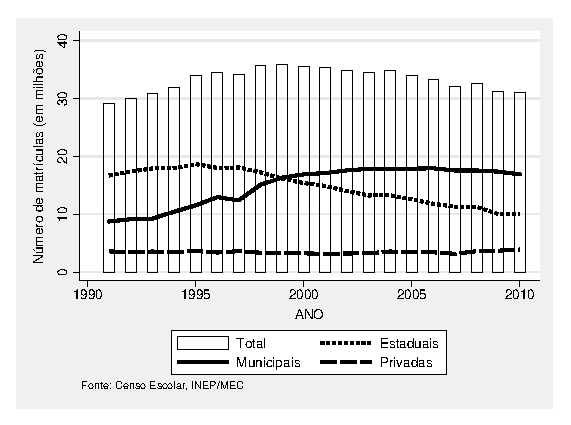
\includegraphics[height=3in]{matriculas_total}
\end{footnotesize}
\end{figure}
 
%\vspace*{1cm} 

%%%%%%%%%%%%%%%%%%%%%%%%%%%%%
%%%%%%%%%%%%%%%%%%%%%%%%%%%%%


Verifica-se que a grande maioria dos alunos est‡ matriculada nas escolas pœblicas, estaduais ou municipais. O nœmero de matr’culas na rede privada de educa‹o fundamental conserva-se praticamente invari‡vel em torno de pouco mais de 3 milh›es. A partir dos nœmeros apresentados na figura \ref{fig:total_matriculas}, pode-se concluir que a grande expans‹o do nœmero de alunos matriculados no ensino fundamental deve-se, quase que exclusivamente, ˆ amplia‹o da rede pœblica de ensino. Particularmente, ˆ expans‹o do nœmero de matriculados em escolas pœblicas municipais. Em 1991, havia cerca de 25 milh›es de alunos matriculados em escolas pœblicas estaduais e municipais. No final da dŽcada de 1990, esse nœmero ultrapassa os 32 milh›es de matriculados. Em 2010, devido a queda no nœmero de matriculados no ensino fundamental, esse nœmero se reduz para pouco mais de 27 milh›es de alunos. 

Dentro da rede pœblica de ensino, verifica-se um expressivo crescimento do nœmero de matr’culas nas escolas municipais. Em 1991, havia aproximadamente, 16, 7 milh›es de alunos matriculados nas escolas estaduais e 8,7 milh›es em escolas municipais. Em 2010, os munic’pios passam a atender aproximadamente 17 milh›es de alunos. Os restantes 10 milh›es de matriculados na rede pœblica encontram-se em escolas mantidas pelos estados. Conclui-se, portanto, que ao longo das duas œltimas dŽcadas, as escolas municipais foram respons‡veis pela incorpora‹o de aproximadamente 15,5  milh›es de alunos. Na medida em que, as redes municipais cresceram, absorvendo tanto matr’culas novas (cerca de 9 milh›es) como parte significativa das matr’culas estaduais (aproximadamente 6,5 milh›es). 

Em suma, o processo que se denomina aqui municipaliza‹o das matr’culas d‡-se tanto por meio da incorpora‹o de novos alunos, como tambŽm por meio da transferncia de matr’culas das escolas pœblicas estaduais para as escolas pœblicas municipais. 

Nota-se ainda que, a municipaliza‹o das matr’culas no ensino fundamental n‹o ocorre paulatinamente ao longo das duas œltimas dŽcadas. Mas, pelo contr‡rio, ele se intensifica a partir de 1996 e parece se estabilizar novamente em 2006. 


%%%%%%%%%%%%%%%%%%%%%%%%%%%%%
%%%%%%%%%%%%%%%%%%%%%%%%%%%%%

\vspace*{1cm} 

\begin{figure}[h]
\centering
\begin{footnotesize}
\caption{Divis‹o das matr’culas do ensino fundamental em escolas privadas e pœblicas estaduais e municipais no Brasil (1991-2010)} 
\label{fig:share_matriculas2}                             
 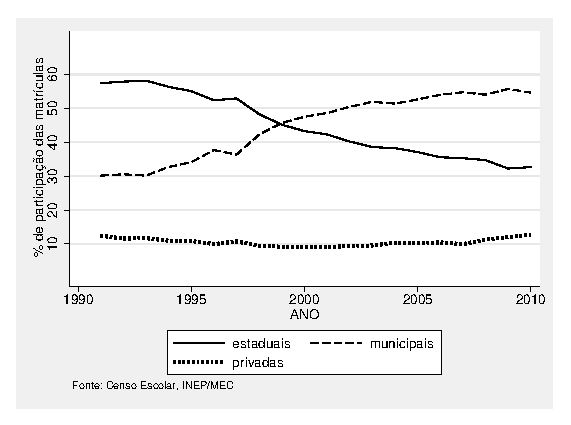
\includegraphics[height=3in]{share_matriculas2}
\end{footnotesize}
\end{figure}
 
%\vspace*{1cm} 

%%%%%%%%%%%%%%%%%%%%%%%%%%%%%
%%%%%%%%%%%%%%%%%%%%%%%%%%%%%


Como pode se inferir a partir da figura \ref{fig:share_matriculas2}, em 1996, apenas 37 por cento dos alunos matriculados no ensino fundamental pœblico no pa’s frequentavam escolas municipais. O restante, 63 por cento, frequentava escolas das redes estaduais de ensino. Dez anos depois, em 2006, tal cen‡rio havia se invertido totalmente. Os munic’pios passaram a atender aproximadamente 60 por cento dos alunos matriculados no ensino pœblico no pa’s. Ademais, cabe ressaltar que, a participa‹o da rede privada de ensino no total de matr’culas do ensino fundamental permanece est‡vel por volta dos 10 por cento ao longo de todo o per’odo compreendido entre os anos 1991 e 2010.


%%%%%%%%%%%%%%%%%%%%%%%%%%%%%
%%%%%%%%%%%%%%%%%%%%%%%%%%%%%

\vspace*{1cm} 

\begin{figure}[h]
\centering
\begin{footnotesize}
\caption{Nœmero de estabelecimentos pœblicos de ensino fundamental  
\newline segundo a dependncia administrativa (1991-2010)} 
\label{fig:estabelecimentos}                             
 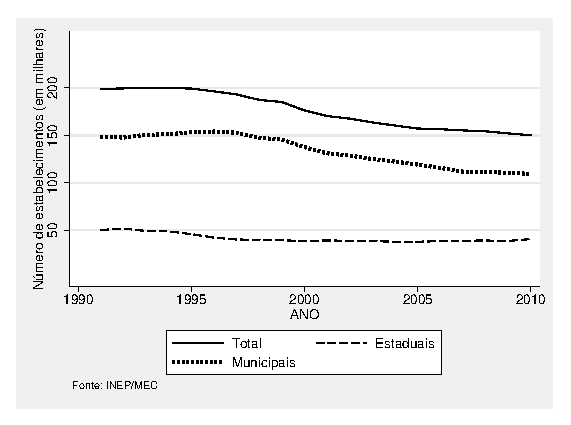
\includegraphics[height=3in]{estabelecimentos}
\end{footnotesize}
\end{figure}
 
%\vspace*{0.5cm} 

%%%%%%%%%%%%%%%%%%%%%%%%%%%%%
%%%%%%%%%%%%%%%%%%%%%%%%%%%%%



\subsection{As escolas}


Outro aspecto do processo de municipaliza‹o das matr’culas do ensino fundamental que merece relevo, Ž que a descentraliza‹o ocorre concomitantemente a uma redu‹o do nœmero de estabelecimentos pœblicos que ofereciam vagas no ensino fundamental, como j‡ foi observado com precis‹o por Leme, Paredes e Souza (2009: 267). A figura \ref{fig:estabelecimentos} exibe o nœmero de estabelecimentos de ensino pœblico, segundo a dependncia administrativa, entre os anos de 1991 e 2010.


Nota-se uma clara queda no nœmero de estabelecimentos de ensino pœblico no per’odo. Em 1991, havia aproximadamente 200 mil escolas pœblicas de ensino fundamental, cerca de 150 mil escolas pœblicas municipais e 50 mil escolas estaduais. Em 2010, o nœmero de estabelecimentos pœblicos de ensino fundamental cai para aproximadamente 150 mil, das quais por volta de 110 mil eram escolas municipais e o restante 40 mil, estaduais. Como pode se observar na figura  \ref{fig:estabelecimentos}, a redu‹o no nœmero de estabelecimentos de ensino se manifesta tanto nas redes escolares estaduais como nas municipais.


\subsection{As turmas}


Uma terceira din‰mica do ensino pœblico no Brasil que deve ser aqui destacada Ž o aumento do nœmero de turmas do ensino fundamental. O aumento das turmas est‡, evidentemente, vinculado a expans‹o das matr’culas e a redu‹o do nœmero de escolas. Houve no per’odo um significativo aumento do nœmero de turmas por estabelecimento, principalmente nas escolas municipais. A partir do dados do Censo Escolar, pode-se inferir que, se por um lado, houve uma redu‹o do nœmero de estabelecimentos, principalmente pela elimina‹o de escolas rurais ou de pequeno porte. Por outro lado, verifica-se um significativo aumento do nœmero de turmas por estabelecimento de ensino. Ou seja, os alunos foram concentrados em escolas maiores.

Conforme pode se observar na figura \ref{fig:turmas}, o nœmero total de turmas se mantŽm praticamente inalterado, em torno de 1,2 milh‹o de turmas no ensino fundamental da rede pœblica. O total do nœmero de turmas nas escolas municipais tem um crescimento de mais de 50 por cento, pulando de aproximadamente 470 mil turmas em 1997 para mais de 720 mil turmas em 2007. De tal sorte que, o nœmero mŽdio de turmas por estabelecimento nas escolas municipais tem um aumento de 3,5 turmas/estabelecimento em 1997 para 5,3 turmas/estabelecimento em 2007.


%%%%%%%%%%%%%%%%%%%%%%%%%%%%%
%%%%%%%%%%%%%%%%%%%%%%%%%%%%%

\vspace*{1cm} 

\begin{figure}[h]
\centering
\begin{footnotesize}
\caption{Nœmero de turmas do ensino fundamental pœblico  
\newline segundo a dependncia administrativa (1991-2010)} 
\label{fig:turmas}                             
 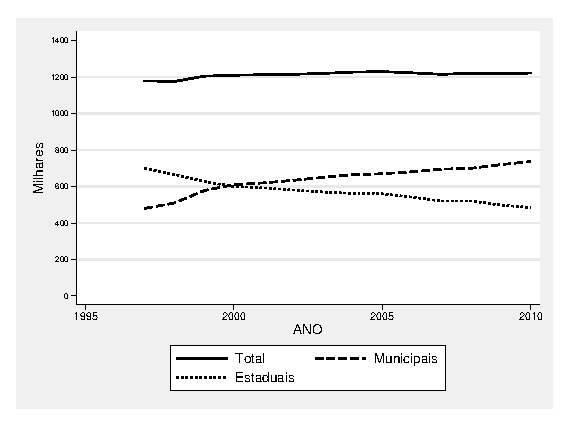
\includegraphics[height=3in]{turmas}
\end{footnotesize}
\end{figure}
 
\vspace*{0.5cm} 

%%%%%%%%%%%%%%%%%%%%%%%%%%%%%
%%%%%%%%%%%%%%%%%%%%%%%%%%%%%



Nas escolas estaduais, por outro lado, esse aumento n‹o se repete. Pelo contr‡rio, havia, em 1997, pouco menos de 600 mil turmas de ensino fundamental nas escolas estaduais. Em 2007, esse total cai para pouco menos de 400 mil turmas. Ou seja, houve uma redu‹o no total de turmas do ensino fundamental de aproximadamente 30 por cento nas escolas estaduais. 
 
Finalmente, cabe destacar que esse expressivo aumento do nœmero de turmas por estabelecimento de ensino que se observa para as escolas municipais n‹o ocasiona um aumento do nœmero mŽdio de alunos por turma. O nœmero mŽdio de alunos por turma para as escolas municipais era de pouco mais de 26 alunos/turma, em 1997. Esse nœmero se mantŽm praticamente est‡vel. Em 2007, encontra-se em pouco mais de 24 alunos/turma. 
 
 
 
 
 
%%%%%%%%%%%%%%%%%%%%%%%%%%%%%
%%%%%%%%%%%%%%%%%%%%%%%%%%%%%


\pagebreak

\section{Dados e MŽtodos}

Os dados utilizados nessa pesquisa provm do Sistema Nacional de Avalia‹o da Educa‹o B‡sica (SAEB), da Prova Brasil e do Censo Escolar da Educa‹o B‡sica. Na presente se‹o do trabalho, s‹o apresentadas as fontes de dados, que s‹o utilizadas em todos os trs exerc’cios de estima‹o do efeito da municipaliza‹o descritos neste cap’tulo. Como discutido anteriormente, a estratŽgia emp’rica proposta neste estudo baseia-se na decomposi‹o de efeito da municipaliza‹o sobre: ($i$) a diferena de desempenho dos alunos de escolas municipais e estaduais nos exames de avalia‹o do SAEB, ($ii$) a proficincia mŽdia das escolas que tiveram seu controle transferido dos estados para os munic’pios; e, finalmente, ($iii$) sobre os indicadores de insumos escolares e rendimento do fluxo escolar dos munic’pios. 

Nas se›es seguintes deste cap’tulo, ap—s apresentar as fontes de dados e algumas estat’sticas descritivas, s‹o apresentadas mais detalhadamente cada uma das an‡lises emp’ricas propostas. Os resultados dessas an‡lises s‹o apresentados separadamente, no sexto cap’tulo do trabalho.

\subsection{O SAEB}

O Sistema Nacional de Avalia‹o da Educa‹o B‡sica (SAEB) foi criado pelo INEP em 1988. Em 1990, foi aplicada a primeira avalia‹o a uma amostra de escolas representativas, para cada unidade da federa‹o, das redes pœblica e privada. A avalia‹o foi repetida em 1993, e, desde ent‹o, o SAEB tornou-se um exame bienal de proficincia, em Matem‡tica (com nfase em resolu‹o de problemas) e em L’ngua Portuguesa (com nfase em leitura), aplicado em amostras de alunos de 4a e 8a sŽries do ensino fundamental e da 3a sŽrie do ensino mŽdio.	

Desde 1995, a tŽcnica de mensura‹o do desempenho dos alunos utilizada no SAEB baseia-se na Teoria de Resposta ao Item (TRI). Uma das grandes vantagens da TRI sobre a Teoria Cl‡ssica das Medidas Ž que a TRI possibilita compara›es de desempenho entre popula›es submetidas a provas que tenham alguns itens em comum, ou, ainda, entre indiv’duos da mesma popula‹o que tenham sido submetidos a provas diferentes. Ou seja, os resultados obtidos a partir da TRI s‹o independentes de grupos e n‹o s‹o afetados pela dificuldade dos testes. A comparabilidade dos resultados Ž garantida pela inclus‹o de itens comuns nos instrumentos de avalia‹o. A utiliza‹o de itens comuns ˆs avalia›es de edi›es anteriores Ž denominada de "equaliza‹o de grupos n‹o equivalentes com itens comuns". Faz-se uso de matrizes de referncia para a constru‹o dos instrumentos de avalia‹o. Essas matrizes funcionam como orienta‹o para a sele‹o dos itens que comp›em os instrumentos de avalia‹o. Dessa maneira, Ž poss’vel comparar o desempenho dos alunos ou das escolas brasileiras ao longo dos anos entre 1995 e 2005 e tentar diagnosticar quais os fatores relevantes ˆ qualidade da educa‹o (INEP, 2008).

TambŽm a partir do SAEB de 1995, os teste s‹o compostos de um total de 169 itens de mœltipla escolha para cada uma das sŽries e das disciplinas avaliadas. Esses itens s‹o divididos em 13 blocos de 13 itens cada, organizados em grupos de trs diferentes combina›es. Isto Ž, combinados trs a trs. Cada combina‹o resulta em um caderno de prova. Ao final do processo combinat—rio, tm-se, portanto, um total de 26 cadernos de provas diferentes. A composi‹o dos cadernos de provas do SAEB baseia-se no modelo de "Blocos Incompletos Balanceados", ou \emph{Balanced Incomplete Block}, no original em ingls. Procura-se, por meio dessa metodologia, compor blocos e cadernos de provas com dificuldades semelhantes e, mais importante, variabilidade e ordenamento dos itens em fun‹o da sua dificuldade (INEP, 2008). 

As figuras  \ref{fig:SAEB} e \ref{fig:SAEB2} apresentam a evolu‹o das proficincias mŽdias em L’ngua Portuguesa e Matem‡tica no SAEB entre os anos de 1995 e 2005. Nas figuras Ž poss’vel observar a trajet—ria descendente dos resultados ao longo do per’odo. Os resultados demonstram uma queda na mŽdia obtida nos exames padronizados de Matem‡tica e L’ngua Portuguesa. Seja na 4a ou 8a sŽrie do ensino fundamental, seja na 3a sŽrie do ensino mŽdio.

%%%%%%%%%%%%%%%%%%%%%%%%%%%%%
%%%%%%%%%%%%%%%%%%%%%%%%%%%%%

%\vspace*{1cm} 

\begin{figure}[h]
\centering
\begin{footnotesize}
\caption{Proficincias mŽdias em L’ngua Portuguesa  nos exames do 
\newline SAEB (1995-2005)} 
\label{fig:SAEB}                             
 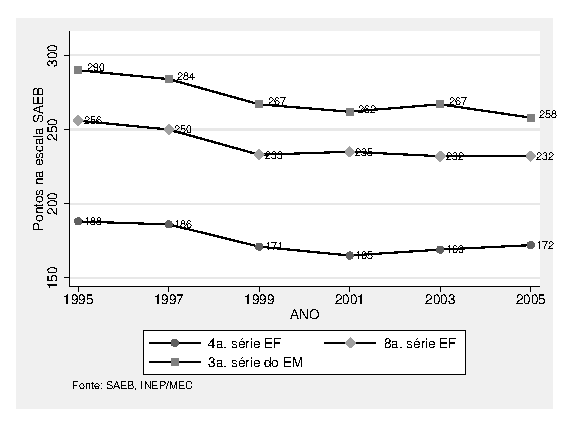
\includegraphics[height=3in]{SAEB}
\end{footnotesize}
\end{figure}
 
%\vspace*{1cm} 

%%%%%%%%%%%%%%%%%%%%%%%%%%%%%
%%%%%%%%%%%%%%%%%%%%%%%%%%%%%

%%%%%%%%%%%%%%%%%%%%%%%%%%%%%
%%%%%%%%%%%%%%%%%%%%%%%%%%%%%

%\vspace*{1cm} 

\begin{figure}[h]
\centering
\begin{footnotesize}
\caption{Proficincias mŽdias em Matem‡tica nos exames do
\newline SAEB (1995-2005)} 
\label{fig:SAEB2}                             
 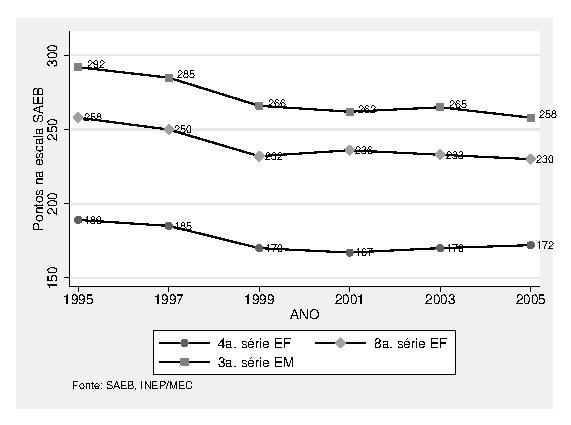
\includegraphics[height=3in]{SAEB2}
\end{footnotesize}
\end{figure}
 
%\vspace*{0.5cm} 

%%%%%%%%%%%%%%%%%%%%%%%%%%%%%
%%%%%%%%%%%%%%%%%%%%%%%%%%%%%

Adicionalmente aos testes padronizados de conhecimento espec’fico, o SAEB tambŽm aplica question‡rios socioecon™micos. Estes question‡rios s‹o respondidos por alunos, professores e diretores das escolas que comp›em ˆ amostra, possibilitando o conhecimento de informa›es mais amplas sobre o sistema educacional, as condi›es das escolas brasileiras e das fam’lias dos estudantes.

Os microdados do SAEB est‹o dispon’veis para os anos de 1995 atŽ 2005. Estes dados podem ser obtidos diretamente do s’tio do INEP na internet. Entretanto, como foi observado por Biondi e Fel’cio \citeyear{biondi_2007_atributos}, h‡ um subgrupo de escolas que se repete nas amostras. De tal sorte que, Ž poss’vel compor um painel de dados com esse subgrupo de escolas que aparecem repetidas vezes nas avalia›es. A montagem dos dados em painel permite acompanhar a evolu‹o dos testes de proficincia e das condi›es socioecon™micas extra’das dos question‡rios respondidos pelos alunos, professores e diretores, para esse subgrupo de escolas que Ž mantido na amostra do SAEB. 

Cabe destacar que, a possibilidade de explorar a metodologia para dados em painel assegura maior precis‹o na investiga‹o dos par‰metros de interesse. As estimativas de vari‡veis regressoras observ‡veis, como o caso, por exemplo, da municipaliza‹o das escolas, baseadas t‹o somente em dados de corte temporal (isto Ž, em  \emph{cross-section}), como Ž bastante comum em trabalhos acadmicos a respeito do efeito de \emph{insumos de educa‹o} no Brasil, n‹o permitem o controle dos efeitos espec’ficos das escolas. Isto Ž, n‹o permitem o controle de caracter’sticas n‹o observ‡veis das escolas. A ausncia de controles dos  efeitos espec’ficos das escolas, por sua vez, pode conduzir a estimativas inconsistentes e enviesadas. Mais especificamente, pode produzir estimativas com problemas de viŽs de vari‡veis omitidas, na medida em que as vari‡veis omitidas (n‹o observadas) estiverem correlacionadas com os demais regressores.

Uma complica‹o adicional ao se trabalhar com os dados do SAEB em painel Ž compatibilizar as respostas dos dicion‡rios de alunos, de professores, de diretores, de escolas e de turmas para os diferentes anos sem invalidar ou abrir m‹o de vari‡veis que s‹o relevantes. A vari‡vel "educa‹o da m‹e", por exemplo, aparece categorizada de forma diversa e incompat’vel entre os diferentes anos. Nesse caso, a solu‹o encontrada foi a recodifica‹o da vari‡vel de forma a harmonizar e compatibilizar as respostas entre os diferentes cortes temporais. 

O ano de 1997, em particular, apresenta complica›es extraordin‡rias. Pois, n‹o apenas a quase totalidade das vari‡veis que comp›em os question‡rios de alunos, professores, diretores e escolas est‹o categorizadas de maneira diversa dos demais cortes temporais, como ainda n‹o h‡ um question‡rio espec’fico para as turmas. Por conseguinte, para 1997, n‹o foi poss’vel obter vari‡veis que fossem pass’veis de compara‹o com os demais anos, que detalhassem a quantidade de alunos presentes na sala, a quantidade de horas de aula por dia, se a turma ficou sem professor por algum per’odo (mais de um ms) e se a turma teve mais de um professor (de matem‡tica ou de portugus) durante o per’odo letivo.

Outros trabalhos \footnote{a esse respeito ver Biondi e Fel’cio, 2007 e \cite{franco_2010_impactos}, entre outros estudos que se valem do uso dos dados do SAEB em painel.} que fizeram uso dos dados do SAEB e se valeram das metodologias para dados em painel, usualmente, reportam os resultados para o painel completo (1997-2005), como tambŽm para um painel mais curto, que exclui as observa›es de 1997. Esse painel mais curto (1999-2005) traz a vantagem de uma maior a harmoniza‹o nas perguntas que comp›em as vari‡veis, o que possibilita a investiga‹o de um maior nœmero de vari‡veis.\footnote{Nesse sentido, foram selecionados dois conjuntos de vari‡veis: (1) aquelas que se repetiam nos question‡rios entre os anos de 1997 e 2005; e (ii) um conjunto mais amplo de vari‡veis que se repetiam nos question‡rios entre os anos de 1999 e 2005.} Ademais, tambŽm Ž maior o nœmero de escolas que se repetem entre os anos de 1999 e 2005, o que garante um melhor balanceamento ao painel.\footnote{ƒ importante observar, como ser‡ comentado mais detalhadamente adiante, que nenhum dos painŽis Ž realmente balanceado, no entanto o painel mais curto (1999-2005) tem um maior nœmero de escolas que se repetem ao longo dos anos.} 

\subsection{O Censo Escolar}

Um dos diferenciais desta tese Ž a utiliza‹o conjunta dos dados do SAEB e do Censo Escolar de forma a incorporar um conjunto mais completo de informa›es a respeito das escolas. O Censo Escolar Ž realizado anualmente pelo INEP em parceria com os governos estaduais e municipais. Sua base de dados contŽm informa›es acerca das escolas, de seus alunos e de seus professores.\footnote{Os dados do Censo Escolar foram agregados a base de dados por meio dos c—digos de m‡scaras das escolas. Esses c—digos, que permitem identificar individualmente as escolas amostradas no SAEB, possibilitam que os dados do SAEB sejam cruzados com as informa›es do Censo Escolar e da Prova Brasil. Os c—digos de m‡scaras das escolas podem ser solicitados ao MEC/INEP. Os dados s‹o cedidos (exclusivamente para fins de pesquisa acadmica) mediante ˆ assinatura de um termo de compromisso de confidencialidade dos dados por parte do pesquisador.} 

Os dados contidos no Censo Escolar possibilitam associar informa›es acerca da infra-estrutura, do tamanho e das condi›es de oferta do ensino nas escolas ˆs informa›es socioecon™micas contidas nos question‡rios do SAEB. Ainda, o Censo Escolar traz informa›es sobre caracter’sticas das escolas, como insumos de produ‹o e resultados escolares,  tais como: taxas de matr’cula, repeti‹o, abandono e defasagem idade-sŽrie nas escolas, composi‹o do corpo docente segundo a modalidade de ensino, n’vel de instru‹o dos professores, nœmero de matr’culas por sŽrie, por turma e por turno, dentre outras informa›es. Vale destacar que, para construir um painel de escolas, os dados do SAEB relativos aos alunos e aos docentes (nos casos onde mais de um professor de uma mesma disciplina respondeu ao question‡rio socioecon™mico) podem ser agregados por escola ou, alternativamente, pode-se tambŽm apenas utilizar uma sŽrie de vari‡veis do tipo \emph{dummy} para se identificar as escolas e trabalhar com os dados desagregados dos alunos. Como, por exemplo, no caso da an‡lise emp’rica conduzida nesta tese a respeito do efeito da rede escolar (se municipal ou estadual) sobre o desempenho dos alunos nos exames de proficincia do SAEB.


\subsection{Vari‡veis e estat’sticas descritivas}

Como j‡ foi mencionado, o SAEB Ž uma pesquisa de avalia‹o em larga escala que tem car‡ter amostral. A maioria das escolas que comp›em a amostra de um corte temporal n‹o se repete no corte consecutivo e, consequentemente, uma parcela consider‡vel das escolas avaliadas n‹o se repete em mais do que 2 anos para os quais o SAEB foi realizado. Assim, para fazer uso adequado das tŽcnicas de an‡lise de dados em painel faz-se necess‡rio seccionar os dados em dois subconjuntos: 

\begin{itemize}

\item Painel "longo": um painel n‹o balanceado de escolas composto por dados do SAEB e do Censo Escolar para os anos 1997, 1999, 2001, 2003 e 2005.

\item Painel "curto": um painel n‹o balanceado de escolas composto por dados do SAEB e do Censo Escolar para os anos 1999, 2001, 2003 e 2005.

\end{itemize}

Desse subconjunto de escolas, foram ainda exclu’das as escolas que s— apareciam uma œnica vez durante o per’odo coberto pela an‡lise (1997-2005): as quais somam aproximadamente 41 por cento da amostra total de escolas avaliadas pelo SAEB. AlŽm disso, tambŽm foram retiradas as escolas federais, que representavam menos de 0.4 por cento do total de escolas que comp›em a amostra do SAEB.   

Evidentemente, a op‹o de restringir a an‡lise a t‹o-somente um subgrupo de escolas -- aquelas que s‹o mantidas nas amostras do SAEB -- enseja a quest‹o de qu‹o representativo seria o subgrupo que comp›e o painel quando comparado a amostra total de escolas que comp›em o SAEB. Nesse sentido, deve-se salientar que a compara‹o de mŽdias dos testes de proficincia nas disciplinas de Portugus e Matem‡tica, entre o total das escolas amostradas e as escolas que comp›em o painel, indica que as œltimas representam, de maneira adequada, o total das escolas. Esse equil’brio concede maior suporte estat’stico ˆs an‡lises realizadas no presente trabalho, baseadas na amostra de escolas comuns entre os anos, e possibilita a extens‹o dos resultados encontrados ˆs demais escolas amostradas no SAEB. Por conseguinte, as inferncias obtidas podem ser estendidas ao universo das escolas brasileiras.

%%%%%%%%%%%%%%%%
\vspace*{1cm} 
\begin{table}[htbp]\centering
\begin{footnotesize}
\def\sym#1{\ifmmode^{#1}\else\(^{#1}\)\fi}
\caption{Profici�ncia SAEB, 4a. s�rie do ensino fundamental   \newline  L�ngua Portuguesa \label{tab:profic_port}}
\begin{tabular}{l*{6}{c}}
\toprule
          &\multicolumn{1}{c}{(1)}&\multicolumn{1}{c}{(2)}&\multicolumn{1}{c}{(3)}&\multicolumn{1}{c}{(4)}&\multicolumn{1}{c}{(5)} &\multicolumn{1}{c}{(6)}\\
          &\multicolumn{1}{c}{SAEB}&\multicolumn{1}{c}{SAEB}&\multicolumn{1}{c}{SAEB}&\multicolumn{1}{c}{Painel}&\multicolumn{1}{c}{Painel} &\multicolumn{1}{c}{Painel}\\
          &\multicolumn{1}{c}{Privadas}&\multicolumn{1}{c}{Estaduais}&\multicolumn{1}{c}{Municipais}&\multicolumn{1}{c}{Privadas}&\multicolumn{1}{c}{Estaduais} &\multicolumn{1}{c}{Municipais}\\

\midrule
1997 &   215,33 &    174,68 &    170,58& 217,64 &    173,71&    168,92  \\
%\addlinespace
1999 &   205,90   &    161,62&    157,34& 208,17   &    161,82&    158,70 \\
%\addlinespa
2001 &   204,72  &  159,35&   153,25&  206,79  &  159,06&   152,50 \\
%\addlinespace
2003 &      212,72&    166,38&   162,96&    212,93&    165,42& 161,17   \\
%\addlinespace
2005 &      209,74&    167,09&    162,85&     211,14&    168,27&    163,54  \\
%\addlinespace

\midrule
\(N\)     &   45.568         &   50.785        &   56.662         &   29.787  & 32.381    & 34.546      \\
\bottomrule
\multicolumn{6}{l}{\footnotesize Fonte: Calculos pr�prios a partir de dados do SAEB/INEP}\\
\end{tabular}
\end{footnotesize}
\end{table}

%%%%%%%%%%%%%%%
%%%%%%%%%%%%%%%%
%\vspace*{1cm} 
\begin{table}[htbp]\centering
\begin{footnotesize}
\def\sym#1{\ifmmode^{#1}\else\(^{#1}\)\fi}
\caption{Profici�ncia SAEB, 4a. s�rie do ensino fundamental   \newline  Matem�tica \label{tab:profic_mat}}
\begin{tabular}{l*{6}{c}}
\toprule
          &\multicolumn{1}{c}{(1)}&\multicolumn{1}{c}{(2)}&\multicolumn{1}{c}{(3)}&\multicolumn{1}{c}{(4)}&\multicolumn{1}{c}{(5)} &\multicolumn{1}{c}{(6)}\\
          &\multicolumn{1}{c}{SAEB}&\multicolumn{1}{c}{SAEB}&\multicolumn{1}{c}{SAEB}&\multicolumn{1}{c}{Painel}&\multicolumn{1}{c}{Painel} &\multicolumn{1}{c}{Painel}\\
          &\multicolumn{1}{c}{Privadas}&\multicolumn{1}{c}{Estaduais}&\multicolumn{1}{c}{Municipais}&\multicolumn{1}{c}{Privadas}&\multicolumn{1}{c}{Estaduais} &\multicolumn{1}{c}{Municipais}\\

\midrule
1997 &   221,51 &    178,35 & 173,88   &224,71  &  176,60 &    171,86  \\
%\addlinespace
1999 &   214,78   &   172,67 &169,61&    216,89& 173,07 &    170,95 \\
%\addlinespa
2001 &   217,74  &169,53  & 163,89&   220,31&  169,57 &163,33\\
%\addlinespace
2003 &      221,25 &173,75    & 169,38& 221,85&167,49&  167,49   \\
%\addlinespace
2005 &      222,86 &     176,37 & 171,19&    225,26&     177,30& 172,06 \\
%\addlinespace

\midrule
\(N\)     &   45.568         &   50.785        &   56.662         &   29.787  & 32.381    & 34.546      \\
\bottomrule
\multicolumn{6}{l}{\footnotesize Fonte: Calculos pr�prios a partir de dados do SAEB/INEP}\\
\end{tabular}
\end{footnotesize}
\end{table}

%%%%%%%%%%%%%%%

As Tabelas \ref{tab:profic_port} e \ref{tab:profic_mat} abaixo trazem a compara‹o de mŽdias nos testes de proficincia em L’ngua Portuguesa e Matem‡tica entre o total de escolas amostradas no SAEB e o subgrupo de escolas repetidas entre os anos 1997 e 2005 inclu’das no painel de dados.

A Tabela \ref{tab:painel} abaixo apresenta o nœmero de escolas segundo a frequncia nos anos e segundo o ano que foram mantidas na subamostra de escolas que comp›em os paines utilizados na presente investiga‹o.

%%%%%%%%%%%%%%%%
\vspace*{1cm} 
\begin{table}[htbp]\centering
\begin{footnotesize}
\def\sym#1{\ifmmode^{#1}\else\(^{#1}\)\fi}
\caption{N�mero de alunos e de escolas por ano e por frequ�ncia em que aparecem nas avalia��es do SAEB (1997-2005) \label{tab:painel}}
\begin{tabular}{l*{6}{c}}
\toprule
                    &\multicolumn{1}{c}{Total de}&\multicolumn{1}{c}{Total de}&\multicolumn{4}{c}{Frequ�ncia de Escolas nas Avalia��es}\\
          &\multicolumn{1}{c}{Alunos}&\multicolumn{1}{c}{Escolas}&\multicolumn{1}{c}{2 anos}&\multicolumn{1}{c}{3 anos}&\multicolumn{1}{c}{4 anos} &\multicolumn{1}{c}{5 anos}\\

\midrule
1997 &   9.407 &    361 & 184   &116  &  51 &    10  \\
%\addlinespace
1999 &   7.906   &   1.216 &705 &    394& 107 &    10 \\
%\addlinespa
2001 &   27.583  &1.798  & 1.140&   528&  120 &10\\
%\addlinespace
2003 &      17.233 &  1.162  & 647& 398& 107&  10   \\
%\addlinespace
2005 &      21.089 &     1.333 & 776&    436&     111& 10 \\
%\addlinespace

\midrule
\(Total\)     &   83.218         &   5.875        &   3.462         &   1.987  & 591    & 50     \\
\bottomrule
\multicolumn{6}{l}{\footnotesize Fonte: Calculos pr�prios a partir de dados do SAEB/INEP}\\
\end{tabular}
\end{footnotesize}
\end{table}

%%%%%%%%%%%%%%%

As seguintes tabelas foram elaboradas a partir da amostra total do SAEB e do painel de escolas que se repetem nas amostras do SAEB entre os anos 1997 e 2005. Nestas tabelas Ž poss’vel cotejar as caracter’sticas de alunos, professores, diretores, turmas e escolas que comp›em a amostra total do SAEB ao subgrupo de escolas que fazem parte do painel. As estat’sticas descritivas, tanto para amostra total do SAEB como tambŽm para o subgrupo de escolas que comp›em o painel, est‹o discriminadas segundo a rede escolar, se privadas ou pœblica, e segundo a dependncia administrativa, se pœblica municipal ou pœblica estadual. 

As estat’sticas descritivas referentes ˆs caracter’sticas dos alunos da 4a. sŽrie do ensino fundamental que foram avaliados em Portugus entres os anos 1997 e 2005 s‹o apresentadas na Tabela \ref{tab:varalunos} abaixo. 

%%%%%%%%%%%%%%%%%%%%%%

\vspace*{1cm} 
\begin{table}[htbp]\centering
\begin{footnotesize}
\def\sym#1{\ifmmode^{#1}\else\(^{#1}\)\fi}
\caption{Vari�veis dos alunos da 4a. s�rie do ensino fundamental   \newline  L�ngua Portuguesa \label{tab:varalunos}}
\begin{tabular}{l*{6}{c}}
\toprule
          &\multicolumn{1}{c}{(1)}&\multicolumn{1}{c}{(2)}&\multicolumn{1}{c}{(3)}&\multicolumn{1}{c}{(4)}&\multicolumn{1}{c}{(5)} &\multicolumn{1}{c}{(6)}\\
          &\multicolumn{1}{c}{SAEB}&\multicolumn{1}{c}{SAEB}&\multicolumn{1}{c}{SAEB}&\multicolumn{1}{c}{Painel}&\multicolumn{1}{c}{Painel} &\multicolumn{1}{c}{Painel}\\
          &\multicolumn{1}{c}{Privadas}&\multicolumn{1}{c}{Estaduais}&\multicolumn{1}{c}{Municipais}&\multicolumn{1}{c}{Privadas}&\multicolumn{1}{c}{Estaduais} &\multicolumn{1}{c}{Municipais}\\

\midrule
Homens &    50,6\% &    50,1\%&    50,3\%& 50,6\% &    49,9\%&    50,1\%  \\
%\addlinespace
Idade: 9 anos &   12,7\%   &    7,1\%&    6,0\% & 12,6\%   &    7,1\%&    6,1\% \\
%\addlinespace
Idade: 10 anos &   63,9\%  &  40,1\%&   35,3\%&  64,2\%  &  40,3\%&   36,0\%  \\
%\addlinespace
Idade: 11 anos &      17,8\%&    23,9\%&    24,9\%& 17,5\%&    23,8\%&    25,1\%    \\
%\addlinespace
Idade: 12 anos ou + &      5,0\%&    28,0\%&    32,9\%&     4,5\%&    27,8\%&    31,8\%   \\
%\addlinespace
Branco  &           50,6\%    &    36,8\% &    35,9\%&  50,9\%    &    36,7\% &    36,0\%   \\
%\addlinespace
Pardo &               35,7\%   &      42,2\% &    41,7\%&  35,7\%   &  42,3\% &    41,7\%   \\
%\addlinespace
Negro &               4,7\% &       12,4\% &      13,7\%&  4,3\% &   12,3\% &      13,6\%      \\
%\addlinespace
Amarelo ou Indigena & 7,9\% &  6,9\% &   7,0\%&  8,0\% &  6,9\% &   6,9\%    \\
%addlinespace
M�e (nunca estudou)   & 0,08\% &  6,2\% &     8,6\%  & 0,07\% &  6,1\% &     8,5\%   \\
%\addlinespace
M�e (1-4 EF)    &           5,4\% &   23,8\% &    28,7\%&    4,9\% &   23,5\% &    28,5\%  \\
%\addlinespace
M�e (5-8 EF)   &         8,9\%     &  19,4\%  &     18,1\%&  8,3\%     &  19,3\%  &     18,2\%  \\
%\addlinespace
M�e (EM)          &        17,1\% &  12,9\%   &   10,4\%  & 16,6\% &  13,1\%   &   10,6\%     \\
%\addlinespace
M�e (superior) &          39,8\%&    9,2\% &    6,7\%&  41,6\%&    9,6\% &    7,1\%  \\
%\addlinespace
M�e (n�o sabe) &      40,6\%  &     39,2\%  &  36,6\%&  40,6\%  &     38,3\%  &  35,5\%  \\
%\addlinespace
Trabalha fora   &        6,1\%   &    16,1\%   &    20,8\% & 5,6\%   &    15,9\%   &    20,2\%  \\
%\addlinespace
Mora c/ pai e m�e &   73,1\% &   63,5\%  &  65,9\%  &  73,5\% &   63,6\%  &  65,4\%    \\
%\addlinespace
Tem computador   &    49,9\%&    10,5\% &   7,8\%   &  52,3\%&    10,8\% &   7,9\%    \\
%\addlinespace
\midrule
\(N\)     &   45.568         &   50.785        &   56.662         &   29.787  & 32.381    & 34.546      \\
\bottomrule
\multicolumn{6}{l}{\footnotesize Fonte: Calculos pr�prios a partir de dados do SAEB/INEP}\\
\multicolumn{6}{l}{\footnotesize Notas: Para o ano de 2005 trata-se de computador com Internet}\\
\end{tabular}
\end{footnotesize}
\end{table}

%\vspace*{1cm} 

%%%%%%%%%%%%%%%%%%%%%%



Algumas estat’sticas descritivas referentes ˆs caracter’sticas dos professores s‹o apresentadas na tabela \ref{tab:varprof} . 

%%%%%%%%%%%%%%%%%%%%%%

%\vspace*{1cm} 
\begin{table}[htbp]\centering
\begin{footnotesize}
\def\sym#1{\ifmmode^{#1}\else\(^{#1}\)\fi}
\caption{Vari�veis dos Professores da 4a. s�rie do ensino fundamental  \label{tab:varprof}}
\begin{tabular}{l*{6}{c}}
\toprule
          &\multicolumn{1}{c}{(1)}&\multicolumn{1}{c}{(2)}&\multicolumn{1}{c}{(3)}&\multicolumn{1}{c}{(4)}&\multicolumn{1}{c}{(5)} &\multicolumn{1}{c}{(6)}\\
          &\multicolumn{1}{c}{SAEB}&\multicolumn{1}{c}{SAEB}&\multicolumn{1}{c}{SAEB}&\multicolumn{1}{c}{Painel}&\multicolumn{1}{c}{Painel} &\multicolumn{1}{c}{Painel}\\
          &\multicolumn{1}{c}{Privadas}&\multicolumn{1}{c}{Estaduais}&\multicolumn{1}{c}{Municipais}&\multicolumn{1}{c}{Privadas}&\multicolumn{1}{c}{Estaduais} &\multicolumn{1}{c}{Municipais}\\

\midrule
Homens &    4,68\% &    5,01\%&    10,3\%& 9,61\% &    9,91\%&    10,1\%  \\
%\addlinespace
at� 30 anos(a)  &           27,4\%    &    26,8\% &    21,7\%&  19,9\%    &    22,1\% &    23,0\%   \\
%\addlinespace
de 30 a 40 anos(b) &               39,1\%   &      41,2\% &    34,7\%&  35,7\%   &  32,3\% &    34,6\%   \\
%\addlinespace
40 anos ou mais(c) &               29,8\% &       30,9\% &      39,7\%&  38,3\% &   32,3\% &      33,6\%      \\
%addlinespace
Curso superior   & 61,8\% &  66,2\% &     41,6\%  & 43,0\% &  46,1\% &     45,5\%   \\
%\addlinespace
Capacita��o(d)    &           82,4\% &   82,7\% &    78,7\%&    74,2\% &   73,5\% &    68,3\%  \\
%\addlinespace
Leciona - 15 anos(e)   &         68,9\%     &  69,4\%  &     48,1\%&  48,3\%     &  49,3\%  &     48,2\%  \\
%\addlinespace
Leciona + 15 anos(f)          &        37,1\% &  39,9\%   &   40,4\%  & 39,6\% &  43,1\%   &   41,6\%     \\

\midrule
%\(N\)     &   45.568         &   50.785        &   56.662         &   29.787  & 32.381    & 34.546      \\
\bottomrule
\multicolumn{6}{l}{\footnotesize Fonte: Calculos pr�prios a partir de dados do SAEB/INEP}\\
\multicolumn{6}{l}{\footnotesize Notas: (a) 1997 a 1999 incluem 30 anos}\\
\multicolumn{6}{l}{\footnotesize (b)1997 a 1999 incluem 40 anos}\\
\multicolumn{6}{l}{\footnotesize (c) 1997 e 1999 a partir dos 41 anos}\\
\multicolumn{6}{l}{\footnotesize (d) 1997 no pr�prio ano}\\
\multicolumn{6}{l}{\footnotesize (e) 2001 h� at� 14 anos}\\
\multicolumn{6}{l}{\footnotesize (f) 2001 h� mais 14 anos}\\

\end{tabular}
\end{footnotesize}
\end{table}

%\vspace*{1cm} 

%%%%%%%%%%%%%%%%%%%%%%

Algumas estat’sticas descritivas referentes ˆs caracter’sticas dos diretores s‹o apresentadas na tabela \ref{tab:vardir}.  
%%%%%%%%%%%%%%%%%%%%%%

%\vspace*{1cm} 
\begin{table}[htbp]\centering
\begin{footnotesize}
\def\sym#1{\ifmmode^{#1}\else\(^{#1}\)\fi}
\caption{Vari�veis dos Diretores \label{tab:vardir}}
\begin{tabular}{l*{6}{c}}
\toprule
          &\multicolumn{1}{c}{(1)}&\multicolumn{1}{c}{(2)}&\multicolumn{1}{c}{(3)}&\multicolumn{1}{c}{(4)}&\multicolumn{1}{c}{(5)} &\multicolumn{1}{c}{(6)}\\
          &\multicolumn{1}{c}{SAEB}&\multicolumn{1}{c}{SAEB}&\multicolumn{1}{c}{SAEB}&\multicolumn{1}{c}{Painel}&\multicolumn{1}{c}{Painel} &\multicolumn{1}{c}{Painel}\\
          &\multicolumn{1}{c}{Privadas}&\multicolumn{1}{c}{Estaduais}&\multicolumn{1}{c}{Municipais}&\multicolumn{1}{c}{Privadas}&\multicolumn{1}{c}{Estaduais} &\multicolumn{1}{c}{Municipais}\\

\midrule
Exp. - 5 anos &   21,4\%    &    20,9\% &  53,1\%    &    54,3\% &    49,4\% &    50,1\%  \\
%\addlinespace
Exp de 5 a 10 anos &           26,6\%    &    25,2\% &    31,3\%&  32,3\%    &    28,3\% &    29,4\%   \\
%\addlinespace
Exp. + 10 anos &               50,1\%   &      52,3\% &    14,5\%&  13,8\%   &  16,6\% &    15,7\%   \\
%\addlinespace
Na escola - 5 anos &               35,5\% &       36,7\% &      68,5\%&  67,3\% &   65,3\% &      64,9\%      \\
%addlinespace
Na escola 5-10 anos  & 25,9\% &  27,2\% &     23,6\%  & 22,1\% &  21,9,4\% &     23,2\%   \\
%\addlinespace
Na escola + 10 anos &           34,4\% &   34,2\% &    6,78\%&    7,31\% &   8,81\% &    9,13\%  \\
%\addlinespace
Elei��o   &         61,3\%     &  63,2\%  &     49,8\%&  51,3\%     &  56,7\%  &     58,1\%  \\
%\addlinespace
Indica��o          &        22,3\% &  23,7\%   &   51,4\%  & 49,7\% &  44,1\%   &   42,3\%     \\
%\addlinespace
Proj. Pedag�gico (n�o)          &        3,61\% &  2,93\%   &   14,3\%  & 13,7\% &  11,2\%   &   10,5\%     \\
%\addlinespace
Proj. Pedag�gico (sec.)     & 9,61\%     &  8,52\%  &     19,7\%&  21,4\%     &  17,2\% &  18,3\%\\
%\addlinespace
Proj. Pedag�gico (dir+prof)     & 82,2\%     &  83,3\%  &     59,3\%&  58,9\%     &  63,2\% &  65,5\%     \\
%\addlinespace
Rotatividade     &    11,1\%     &  10,2\%  &     28,8\%&  28,3\%     &  25,5\%  &     24,9\%      \\
%\addlinespace
Prof. faltosos     &     6,61\%     &  6,43\%  &     22,7\%&  23,1\%     &    19,9\%  &     20,1\%     \\
%\addlinespace

\midrule
%\(N\)     &   45.568         &   50.785        &   56.662         &   29.787  & 32.381    & 34.546      \\
\bottomrule
\multicolumn{6}{l}{\footnotesize Fonte: C�lculos pr�prios a partir de dados do SAEB/INEP}\\
\end{tabular}
\end{footnotesize}
\end{table}

%\vspace*{1cm} 

%%%%%%%%%%%%%%%%%%%%%%



Algumas estat’sticas descritivas referentes ˆs caracter’sticas das turmas s‹o apresentadas na tabela \ref{tab:varturmas}.   
%%%%%%%%%%%%%%%%%%%%%%

%\vspace*{1cm} 
\begin{table}[htbp]\centering
\begin{footnotesize}
\def\sym#1{\ifmmode^{#1}\else\(^{#1}\)\fi}
\caption{Vari�veis das Turmas \label{tab:varturmas}}
\begin{tabular}{l*{6}{c}}
\toprule
          &\multicolumn{1}{c}{(1)}&\multicolumn{1}{c}{(2)}&\multicolumn{1}{c}{(3)}&\multicolumn{1}{c}{(4)}&\multicolumn{1}{c}{(5)} &\multicolumn{1}{c}{(6)}\\
          &\multicolumn{1}{c}{SAEB}&\multicolumn{1}{c}{SAEB}&\multicolumn{1}{c}{SAEB}&\multicolumn{1}{c}{Painel}&\multicolumn{1}{c}{Painel} &\multicolumn{1}{c}{Painel}\\
          &\multicolumn{1}{c}{Privadas}&\multicolumn{1}{c}{Estaduais}&\multicolumn{1}{c}{Municipais}&\multicolumn{1}{c}{Privadas}&\multicolumn{1}{c}{Estaduais} &\multicolumn{1}{c}{Municipais}\\

\midrule
Sem prof de mat. &   3,78\%    &    3,92\% &    6,1\%&  5,9\%    &    4,35\% &    4,64\%   \\
%\addlinespace
Apenas 1 prof mat &           88,3\%    &    89,2\% &    74,3\%&  75,5\%    &    78,3\% &    76,4\%   \\
%\addlinespace
2 ou + prof mat &               7,35\%   &      8,72\% &    16,5\%&  17,8\%   &  15,2\% &    14,7\%   \\
%\addlinespace
Sem prof port &               3,8\% &       3,9\% &      6,6\%&  7,4\% &   5,3\% &      4,9\%      \\
%addlinespace
Apenas 1 prof port  & 85,2\% &  87,2\% &     73,6\%  & 78,0\% &  78,4\% &     77,6\%   \\
%\addlinespace
2 ou mais prof port &           6,4\% &   6,7\% &    15,7\%&    14,3\% &   13,7\% &    12,8\%  \\
%\addlinespace
At� 4 horas/dia   &         39,6\%     &  36,3\%  &     56,2\%&  58,4\%     &  47,5\%  &     48,9\%  \\
%\addlinespace
De 4 a 5 horas/dia          &        64,2\% &  69,5\%   &   39,4\%  & 39,7\% &  37,1\%   &   38,3\%     \\
%\addlinespace
+ de 5 horas/dia          &        2,2\% &  2,3\%   &   4,3\%  & 3,5\% &  4,3\%   &   4,7\%     \\
%\addlinespace
No. m�dio de alunos     &        25,8 &  27,5   &   32,8  & 34,1 &  30,6   &   31,7     \\
%\addlinespace
\midrule
%\(N\)     &   45.568         &   50.785        &   56.662         &   29.787  & 32.381    & 34.546      \\
\bottomrule
\multicolumn{6}{l}{\footnotesize Fonte: C�lculos pr�prios a partir de dados do SAEB/INEP}\\
\multicolumn{6}{l}{\footnotesize Notas: N�o h� question�rio para turmas no SAEB 1997}\\

\end{tabular}
\end{footnotesize}
\end{table}

%\vspace*{1cm} 

%%%%%%%%%%%%%%%%%%%%%%

Algumas estat’sticas descritivas referentes ˆs caracter’sticas das escolas s‹o apresentadas na tabela \ref{tab:varescolas} .  


%%%%%%%%%%%%%%%%%%%%%%

%\vspace*{1cm} 
\begin{table}[htbp]\centering
\begin{footnotesize}
\def\sym#1{\ifmmode^{#1}\else\(^{#1}\)\fi}
\caption{Vari�veis das Escolas \label{tab:varescolas}}
\begin{tabular}{l*{6}{c}}
\toprule
          &\multicolumn{1}{c}{(1)}&\multicolumn{1}{c}{(2)}&\multicolumn{1}{c}{(3)}&\multicolumn{1}{c}{(4)}&\multicolumn{1}{c}{(5)} &\multicolumn{1}{c}{(6)}\\
          &\multicolumn{1}{c}{SAEB}&\multicolumn{1}{c}{SAEB}&\multicolumn{1}{c}{SAEB}&\multicolumn{1}{c}{Painel}&\multicolumn{1}{c}{Painel} &\multicolumn{1}{c}{Painel}\\
          &\multicolumn{1}{c}{Privadas}&\multicolumn{1}{c}{Estaduais}&\multicolumn{1}{c}{Municipais}&\multicolumn{1}{c}{Privadas}&\multicolumn{1}{c}{Estaduais} &\multicolumn{1}{c}{Municipais}\\

\midrule
Rural &   1,07\%    &    0,91\% &  26,1\%    &    27,1\% &    16,2\% &    13,7\%  \\
%\addlinespace
Biblioteca &           86,2\%    &    91,3\% &    51,5\%&  56,2\%    &    58,8\% &    59,1\%   \\
%\addlinespace
Lab. inform�tica &               70,1\%   &      76,3\% &    14,2\%&  13,5\%   &  17,8\% &    20,3\%   \\
%\addlinespace
Lab. ci�ncias &               56,3\% &       52,1\% &      9,50\%&  8,37\% &   15,3\% &      14,9\%      \\
%addlinespace
Qd. esportes  & 75,6\% &  87,1\% &     43,1\%  & 42,0\% &  51,9\% &     48,9\%   \\
%\addlinespace
Merenda &           9,41\% &   8,65\% &    96,45\%&    98,1\% &   98,3\% &    96,3\%  \\
%\addlinespace
Transporte  &         6,32\%     &  6,27\%  &     64,8\%&  67,9\%     &  41,7\%  &     40,3\%  \\
%\addlinespace
\midrule
\(N\)     &   1.029         &   3.764        &   2.036         &   843  & 1565    & 968      \\
\bottomrule
\multicolumn{6}{l}{\footnotesize Fonte: C�lculos pr�prios a partir de dados do SAEB/INEP}\\
\end{tabular}
\end{footnotesize}
\end{table}

%\vspace*{1cm} 

%%%%%%%%%%%%%%%%%%%%%%


O ponto fundamental que se gostaria de destacar da leitura das tabelas 4, 5, 6 e 7, Ž que a compara‹o entre as colunas 1, 2 e 3 das referidas tabelas, que trazem as estat’sticas descritivas da amostra total do SAEB, ˆs colunas 4, 5 e 6, que trazem as estat’sticas descritivas para o subgrupo de escolas que comp›em o painel, demonstra que n‹o h‡ problemas aparentes de sele‹o nos bancos de dados desenvolvidos no presente estudo.


%%%%%%%%%%%%%%%%%%%%%%%%%%%%%%%%%
%%%%%%%%%%%%%%%%%%%%%%%%%%%%%%%%%


\subsection{Metodologia}

A pergunta b‡sica que o presente estudo pretende responder Ž: o n’vel de governo importa para a qualidade da pol’tica pœblica? No caso espec’fico da an‡lise da municipaliza‹o da educa‹o fundamental no Brasil, essa pergunta pode ser reformulada nas seguintes palavras: O n’vel de governo importa para a qualidade da pol’tica educacional oferecida ˆ popula‹o? Como j‡ comentado no primeiro cap’tulo, a descentraliza‹o pode ser apontada como uma das principais pol’ticas governamentais para o ensino fundamental implementadas no Brasil nos œltimos anos. Entretanto, existe ainda muita controvŽrsia a respeito dos efeitos da municipaliza‹o sobre a qualidade do ensino pœblico oferecido no Brasil.  

Para responder essa pergunta b‡sica, a estratŽgia emp’rica adotada no presente estudo consiste em examinar o diferencial de desempenho entre as redes pœblicas de ensino. Mais importante, busca-se examinar o efeito da municipaliza‹o das matr’culas e gastos em educa‹o sobre: 

\begin{itemize}

\item o desempenho escolar do alunos das redes pœblicas municipais e estaduais;

\item o desempenho das escolas que foram transferidas dos estados para os munic’pios;

\item e, finalmente, sobre o desempenho das redes escolares.

\end{itemize}

Esta escolha deriva do pressuposto de que os efeitos da municipaliza‹o podem se fazer sentir de forma diversa sobre os alunos, as escolas e os munic’pios. Por conseguinte, a pergunta inicial acerca efeito da municipaliza‹o sobre a qualidade da educa‹o Ž desdobrada em perguntas espec’ficas acerca:

\begin{itemize}

\item do efeito da municipaliza‹o sobre os alunos, tais como: existe alguma diferena na proficincia dos alunos de escolas pœblicas municipais e escolas pœblicas estaduais? Qual a magnitude dessa diferena? Essa diferena pode ser atribu’da a disparidades nos recursos familiares do alunado, ou deve-se a disparidades nos insumos escolares?

\item do efeito da municipaliza‹o sobre as escolas, tais como: a municipaliza‹o das escolas tem algum impacto sobre a proficincia mŽdia de seus alunos? Qual a diferena na proficincia mŽdia das escolas que foram transferidas do estado para o munic’pio \emph{vis-ˆ-vis} as escolas que permaneceram sobre controle estatal ou municipal?

\item do efeito da municipaliza‹o sobre as redes municipais de ensino pœblico: qual o efeito da expans‹o das matriculas municipais sobre os insumos escolares e as taxas de rendimento do fluxo escolar das coortes nos munic’pios brasileiros?

\end{itemize}


Idealmente, para se responder a tais perguntas poder-se-ia comparar os mesmos alunos e escolas em duas situa›es distintas: primeiramente, sob a gest‹o estadual e, posteriormente, sob a gest‹o municipal, mantendo-se tudo o mais constante. Isto Ž, num desenho \emph{"experimental"}  de pesquisa buscar-se-ia comparar a situa‹o dos mesmos alunos, escolas e munic’pios antes e depois da descentraliza‹o, mantendo-se constantes ao longo do tempo todas as demais vari‡veis que podem afetar os resultados educacionais. Nesse exerc’cio hipotŽtico, poder-se-ia simplesmente comparar a situa‹o prŽ-tratamento -- antes da descentraliza‹o -- com o situa‹o p—s-tratamento -- depois da descentraliza‹o -- para se verificar como se comportariam os alunos, as escolas e os indicadores educacionais dos munic’pios sob o controle municipal e sob o controle estadual. Como foi observado por Leme, Paredes e Souza (2009), a diferena entre essas duas situa›es Ž o que se  denomina de  \emph{efeito da municipaliza‹o}.

Evidentemente, esse Ž t‹o somente um exerc’cio hipotŽtico. Na pr‡tica, n‹o se pode observar essas duas situa›es ao mesmo tempo. Isto Ž, na realidade n‹o se pode comparar ao mesmo tempo uma situa‹o observada, como, por exemplo, o desempenho acadmico dos alunos numa escola sob controle municipal, com seu contrafactual, o desempenho dos mesmos alunos na (mesma) escola sob controle estadual.

Portanto, um dos desafios n‹o triviais do presente estudo, como, ali‡s, de todas as pesquisas de avalia‹o de impacto de pol’ticas pœblicas (educacionais ou n‹o), Ž na ausncia de dados experimentais ser justamente capaz de construir esse \emph{"contrafactual"} a partir de dados observados de diferentes alunos e escolas ao longo do tempo. 

As bases de dados em painel do SAEB e do Censo Escolar, afortunadamente,  possibilitam a constru‹o de um  \emph{"contrafactual estat’stico"}, que seguramente n‹o assevera a existncia de rela›es causais robustas como aquelas erigidas por meio do emprego de dados experimentais; mas, por certo, Ž capaz de fornecer evidncias s—lidas acerca da prevalncia e da magnitude do efeito da municipaliza‹o, seja por meio emprego de vari‡veis de controle para as caracter’sticas observ‡veis dos alunos e das escolas, seja por meio do controle dos efeitos espec’ficos das vari‡veis n‹o observadas das escolas ou dos munic’pios.

Vale observar, no entanto, que o presente estudo n‹o se encontra totalmente desprovido de problemas decorrentes da utiliza‹o de dados observados como subs’dio emp’rico para o estabelecimento de proposi›es e inferncias causais. Como se comentar‡ adiante, Ž razo‡vel admitir que h‡ caracter’sticas n‹o observ‡veis dos alunos ou das escolas que tambŽm influenciam o aprendizado e, por conseguinte, os resultados educacionais e que podem estar correlacionadas com a descentraliza‹o cujo efeito se pretende captar. Particularmente, o terceiro exerc’cio de estima‹o do efeito da municipaliza‹o no munic’pios Ž possivelmente acometido por problemas decorrentes da utiliza‹o de regressores end—genos. 

A seguir s‹o detalhados os procedimentos metodol—gicos dos trs exerc’cios de estima‹o do efeito da municipaliza‹o das matr’culas e dos gastos educacionais sobre: os alunos, as escolas e os munic’pios, respectivamente.

\subsubsection{O desempenho escolar dos alunos: o n’vel de governo importa?}

Uma primeira pergunta diz respeito a diferena na proficincia dos alunos matriculados nas redes pœblicas estaduais e municipais. H‡, de fato, um diferencial de desempenho entre os alunos das redes estaduais e municipais? Secundariamente, tambŽm se procura investigar se a diferena de desempenho entre alunos de escolas pœblicas estaduais e escolas pœblicas municipais pode ser atribu’da a diferenas nos recursos familiares, ou a diferenas nos insumos escolares, ou ainda a diferenas em outras caracter’sticas observ‡veis dos professores, diretores e turmas.

A estratŽgia emp’rica utilizada nesta an‡lise consiste em tirar proveito dos dados em painel, que permitem o controle dos efeitos espec’ficos n‹o observ‡veis das escolas. Pretende-se com esse exerc’cio simplesmente observar se h‡, de fato, uma diferena estatisticamente significante na proficincia em l’ngua portuguesa e matem‡tica dos alunos de 4a. sŽrie matriculados em escolas das redes estaduais e municipais. Est‡ consolidado na literatura sobre o tema \cite{glewwe_chapter_2006} \cite{hanushek_school_1996} que, as caracter’sticas socioecon™micas dos alunos est‹o altamente correlacionadas com o desempenho acadmico. Portanto, estas caracter’sticas, juntamente com outras caracter’sticas observ‡veis dos professores, do diretores, das turmas e da escola s‹o inclu’dos nas an‡lises estat’sticas como vari‡veis de controle. 

As tŽcnicas de an‡lise de dados em painel de M’nimos Quadrados Ordin‡rios agrupados (MQA), Efeitos Fixos (EF) e Efeitos Aleat—rios (EA) foram empregadas neste exerc’cio para se estimar a equa‹o \ref{eq:equac1}  abaixo, que modela o desempenho dos alunos de 4a. sŽrie do ensino fundamental nas provas de Matem‡tica e L’ngua Portuguesa do SAEB:

\begin{equation}
 Y_{ijr}^{t} = \alpha_0 + \beta_1 EST_{ij}^{t}  + \beta_2 A_{ijr}^{t} + \beta_3 P_{ijr}^{t} + \beta_4 D_{ijr}^{t} + \beta_5 T_{ijr}^{t} + \beta_6 E_{ijr}^{t} +  \theta_{i}  + \epsilon_{ikr}^{t} \label{eq:equac1}
\end{equation}

Onde:
\begin{itemize}
\item $Y_{ijr}^{t}$ Ž a proficincia do aluno $i$, na escola $j$, da rede $r$, no tempo $t$
\item$\alpha_0$ Ž uma constante
\item$EST_{ijr}^{t}$ Ž uma vari‡vel do tipo $dummy$ que indica se a escola $j$, do aluno $i$,  no tempo $t$ est‡ sob controle do estado
\item$A_{ijr}^{t}$ Ž o vetor de caracter’sticas do aluno $i$, na escola $j$, da rede $r$, no tempo $t$
\item$P_{ijr}^{t}$ Ž o vetor de caracter’sticas do professor do aluno $i$, na escola $j$, da rede $r$, no tempo $t$
\item$D_{ijr}^{t}$ Ž o vetor de caracter’sticas do diretor do aluno $i$, na escola $j$, da rede $r$, no tempo $t$
\item$T_{ijr}^{t}$ Ž o vetor de caracter’sticas da turma do aluno $i$, na escola $j$, da rede $r$, no tempo $t$
\item$E_{ijr}^{t}$ Ž o vetor de caracter’sticas de infraestrututa da escola do aluno $i$, na escola $j$, da rede $r$, no tempo $t$
\item$\theta_{i}$ Ž o efeito espec’fico n‹o observado da escola
\item$\epsilon_{ijr}^{t}$ Ž o termo de erro aleat—rio 
\end{itemize}

O par‰metro de interesse aqui Ž dado por $\beta_1$, o qual indica a diferena de desempenho acadmico entre os alunos matriculados nas escolas estaduais e municipais. O vetor de par‰metros de controles $\beta'$, tal que $\beta'$ = ($\beta'_2$ $\beta'_3$ $\beta'_4$ $\beta'_5$ $\beta'_6$), reporta as rela›es condicionais dos insumos escolares sobre o desempenho dos alunos. A equa‹o \ref{eq:equac1} Ž a fun‹o de produ‹o da educa‹o, tal como conhecida na literatura  \cite{hanushek_education_1994}.

Ap—s se verificar se existe mesmo diferena entre as proficincias mŽdias de estudantes da redes pœblicas estaduais e municipais, busca-se, ent‹o examinar se essa diferena de desempenho pode ser atribu’da a disparidades nos fatores que podem afetar o rendimento acadmico dos alunos. Isto Ž, procura-se investigar se a diferena de rendimento escolar deve-se ˆ um problema de sele‹o dos alunos entre as redes ou, pelo contr‡rio, deve-se a desigualdades nos insumos escolares das redes pœblicas estaduais e municipais.

Para tanto, se ajustou um modelo de regress‹o probabil’stica, dado pela equa‹o \ref{eq:equacprobit}, que busca captar a correla‹o entre os atributos observ‡veis dos alunos, do ambiente familiar, das escolas, dos professores e diretores e a probabilidade de estarem vinculados ˆs redes pœblicas municipais.


\begin{equation}
 MUNI_{j}^{t} = \alpha_0 + \beta_1A_{ijr}^{t} + \beta_2 P_{ijr}^{t} + \beta_3 D_{ijr}^{t} + \beta_4 T_{ijr}^{t} + \beta_6 E_{ijr}^{t} +  UF_{j}  + t_{t} +  \epsilon_{ikr}^{t} \label{eq:equacprobit}
\end{equation}

Na equa‹o \ref{eq:equacprobit}:
\begin{itemize}
\item $MUNI_{ij}^{t}$ Ž uma vari‡vel do tipo $dummy$ que identifica se a escola $j$ est‡ sob o controle do munic’pio no tempo $t$
\item$\alpha_0$ Ž uma constante
\item$A_{ijr}^{t}$ Ž o vetor de caracter’sticas do aluno $i$, na escola $j$, da rede $r$, no tempo $t$
\item$P_{ijr}^{t}$ Ž o vetor de caracter’sticas do professor do aluno $i$, na escola $j$, da rede $r$, no tempo $t$
\item$D_{ijr}^{t}$ Ž o vetor de caracter’sticas do diretor do aluno $i$, na escola $j$, da rede $r$, no tempo $t$
\item$T_{ijr}^{t}$ Ž o vetor de caracter’sticas da turma do aluno $i$, na escola $j$, da rede $r$, no tempo $t$
\item$E_{ijr}^{t}$ Ž o vetor de caracter’sticas de infraestrututa da escola do aluno $i$, na escola $j$, da rede $r$, no tempo $t$
\item$UF_{j}$ Ž Ž um conjunto de vari‡veis do tipo $dummy$ indicador da UF 
\item$t_{t}$ Ž um conjunto de vari‡veis do tipo $dummy$ indicador do ano
\item$\epsilon_{ijr}^{t}$ Ž o termo de erro aleat—rio 
\end{itemize}



\subsubsection{O efeito da municipaliza‹o nas escolas}

Esta segunda parte da an‡lise emp’rica busca responder a pergunta a respeito da diferena que a mudana do n’vel de governo pode exercer sobre o desempenho mŽdio das escolas. Ou seja,  procura-se  estimar, por meio da metodologia de diferena-em-diferenas, o efeito da municipaliza‹o sobre as escolas que foram transferidas da gest‹o estadual para a gest‹o municipal. Procura-se examinar se houve algum impacto na proficincia mŽdia dos alunos dessas escolas decorrente da transferncia do controle da gest‹o escolar. Para tanto, foram agregados ˆ base de dados do painel de escolas os dados da Prova Brasil de 2007. Como mencionado, o SAEB Ž um exame de avalia‹o de base amostral estratificada (e aleat—ria) das escolas, representativa para os estados e as redes de ensino. A Prova Brasil Ž um exame de avalia‹o em proficincia em l’ngua portuguesa e matem‡tica obrigat—rio para todas as escolas pœblicas do pa’s. A Prova Brasil foi aplicada em 2005 e 2007. A presente an‡lise emp’rica vale-se t‹o somente da base de dados da Prova Brasil para o ano de 2007. 

O mŽtodo de estima‹o por diferena-em-diferenas foi inicialmente aplicado em Card \citeyear{card_impact_1990} e, posteriormente, descrito em Angrist e Krueger \citeyear{angrist_empirical_1999}. No Brasil, foi aplicado por Andrade e colaboradores \citeyear{andrade_freerider_2008} para analisar o impacto do FUNDEF sobre a taxa de reprova‹o dos alunos, por Menezes-Filho e Pazello \citeyear{menezes-filho_teachers_2007} na investiga‹o dos impactos do FUNDEF sobre os sal‡rios dos professores e o aprendizado dos alunos, em Franco e Menezes-Filho \citeyear{franco_2010_impactos} para estimar o impacto do FUNDEF sobre os indicadores educacionais e, finalmente,  por Leme, Paredes e Souza \citeyear{leme_municipalizacao_2009} para se estimar o efeito da municipaliza‹o sobre os resultados educacionais. A abordagem adotada no presente estudo Ž similar ˆquelas utilizadas em Menezes-Filho e Pazello \citeyear{menezes-filho_teachers_2007} e em Leme, Parede e Souza \citeyear{leme_municipalizacao_2009}. 

Inicialmente, buscou-se construir um painel de escolas, em que se identifica a mesma escola pœblica (municipal ou estadual) em dois pontos no tempo: o per’odo inicial, que corresponde aos testes do SAEB para os anos de 1997, 1999, 2001, 2003 e 2005; e um per’odo final, que corresponde ˆ Prova Brasil de 2007. Dessa forma, s‹o montados, na verdade, painŽis de escolas por pares de anos 1997-2007, 1999-2007, 2001-2007, 2003-2007 e 2005-2007. Uma vez montado esse painel de escolas pœblicas de ensino fundamental por pares de anos, as escolas s‹o classificadas de acordo com a rede de ensino a que pertencem -- municipal  ou estadual -- nos anos iniciais e no ano final. Assim, s‹o compostos trs grupos de escolas: um primeiro grupo controle de escolas que estavam sob gest‹o do estado no ano inicial e que permaneceram sob o estado no ano final, o grupo EE; um segundo grupo controle de escolas que eram municipais no ano inicial e permaneceram municipais no ano final, o grupo MM; e, finalmente, um grupo de tratamento para aquelas escolas que eram estaduais no ano inicial e foram transferidas para o controle dos munic’pios no ano final, o grupo EM\footnote{Existe ainda a possibilidade de um quarto grupo: aquele formado pelas escolas que foram estadualizadas; isto Ž, foram transferidas da gest‹o municipal para a estadual. Identificou-se apenas um nœmero muito reduzido de escolas que passaram por esse processo de centraliza‹o. Este grupo foi, portanto, descartado da presente an‡lise.}. Assim, todas as escolas que aparecem nesse painel foram observadas pelo menos em dois pontos no tempo.

A tabela \ref{tab:painel_diff} traz o nœmero de escolas que comp›em esse painel. 

%%%%%%%%%%%%%%%%
 \begin{table}[htbp]\centering
\begin{footnotesize}
\def\sym#1{\ifmmode^{#1}\else\(^{#1}\)\fi}
\caption{N�mero de  escolas por ano no painel (1997-2007) \label{tab:painel_diff}}
\begin{tabular}{l*{4}{c}}
\toprule
                  &\multicolumn{1}{c}{EE}&\multicolumn{1}{c}{EM}&\multicolumn{1}{c}{MM}&\multicolumn{1}{c} {Total} \\

\midrule
1997 &   206 &    9 & 256   &  471\\
%\addlinespace
1999 &   538   &   33 &794 & 1.365\\
%\addlinespa
2001 &   679  & 40  & 880& 1.599\\
%\addlinespace
2003 &      725 &  36  & 795&1.556 \\
%\addlinespace
2005 &      695 &     21 & 696&    1.412 \\
%\addlinespace
2007 &      1726 &   86 & 2171&   3.722 \\
%\addlinespace

\midrule
\(Total\)     &   3.452         &   550        &   3.442         &   7.444     \\
\bottomrule
\multicolumn{5}{l}{\footnotesize Fonte: C�lculos pr�prios}\\
\multicolumn{5}{l}{\footnotesize a partir de dados do MEC/INEP}\\

\end{tabular}
\end{footnotesize}
\end{table}


%%%%%%%%%%%%%%%%

Na presente an‡lise, o efeito da municipaliza‹o que se pretende estimar Ž exatamente o efeito mŽdio do grupo EM em compara‹o com os grupos controle EE e MM. Isto Ž, trata-se da diferena nas proficincias mŽdias do grupo de escolas que foi transferido do controle estadual para o controle municipal cotejada ˆ diferena nas proficincias mŽdias dos grupos  de escolas que permaneceram sob o controle dos estados e munic’pios. Uma observa‹o importante Ž que o efeito estimado da municipaliza‹o das escolas n‹o leva em conta o tempo em que as escolas do grupo de tratamento (EM) estiveram sob controle dos munic’pios. Ou seja, a an‡lise ignora o tempo de exposi‹o ˆ gest‹o municipal.

A estima‹o por diferena-em-diferenas baseia-se na compara‹o das diferenas no desempenho mŽdio nos exames do SAEB em matem‡tica e l’ngua portuguesa entre o grupo de tratamento e os dois grupos controle EE e MM. Intuitivamente, a estima‹o por diferena-em-diferenas Ž a compara‹o das mudanas ao longo do per’odo de 1997 a 2007 na proficincia mŽdia das escolas que foram municipalizadas (grupo EM) com as mudanas ao longo do mesmo per’odo na proficincia mŽdia das escolas que permaneceram sob controle dos estados (grupo EE) e dos munic’pios (grupo MM). 

A equa‹o  \ref{eq:equac2} abaixo procura modelar efeito da municipaliza‹o sobre a proficincia mŽdia das escolas que foram transferidas da gest‹o estadual para a gest‹o municipal, quando comparadas ˆs escolas que n‹o sofreram mudanas quanto ˆ dependncia administrativa a qual se encontram subordinadas.


\begin{equation}
 Y_{ijr}^{t} = \alpha_0 + \beta_1 EM_{ij}  + \beta_2 T_{ij} + \beta_3 EM_{ij} * T_{ij} + \theta_{i}  +  \sum x_{is} + \epsilon_{ik}^{t} \label{eq:equac2}
\end{equation}



Na equa‹o \ref{eq:equac2}:
\begin{itemize}
\item $Y_{ijr}^{t}$ Ž a proficincia do aluno $i$, na escola $j$, da rede $r$, no tempo $t$
\item$\alpha_0$ Ž uma constante
\item$EM_{ij}$ Ž uma vari‡vel do tipo $dummy$ que indica se a escola $j$, do aluno $i$,  migrou do controle do estado para o controle munic’pio no decurso do per’odo de 1997 a 2007
\item$T_{ij}$ Ž uma vari‡vel do tipo $dummy$, $T_{ij}$ = 0 se o ano = 1997, 1999, 2001, 2003 ou 2005 e $T_{ij}$ = 1 se o ano = 2007
\item$x_{ij}$ Ž o vetor de caracter’sticas do aluno $i$, na escola $j$,
\item$\theta_{i}$ Ž o efeito espec’fico n‹o observado da escola
\item$\epsilon_{ij}^{t}$ Ž o termo de erro aleat—rio 
\end{itemize}

Primeiramente, Ž necess‡rio notar que a proficincia mŽdia das escolas dos grupos controle e do grupo tratamento para o per’odo inicial ($T_{ij}$ = 0) e para o per’odo final ($T_{ij}$ = 1) Ž definida conforme as equa›es a seguir:

para o grupo controle EE:
\begin{eqnarray} 
\mbox{$t_{ij}$=0:}& & \bar{EY_{ij}^{t}}  [EM_{ij} = 0, T_{ij} = 0,  \theta_{j}^{EE}]  = \beta_0 +  \theta_{j}^{EE}
\label{eq:equac3}   \\ 
\mbox{$t_{ij}$=1:}& &\bar{EY_{ij}^{t}}  [EM_{ij} = 0, T_{ij} = 1,  \theta_{j}^{EE}]  = \beta_0 + \beta_2 +  \theta_{j}^{EE}
\label{eq:equac4}
\end{eqnarray}
para o grupo controle MM:
\begin{eqnarray}
\mbox{$t_{ij}$=0:}& & \bar{EY_{ij}^{t}}  [EM_{ij} = 0, T_{ij} = 0,  \theta_{j}^{MM}]  = \beta_0 +  \theta_{j}^{MM}
\label{eq:equac5}   \\ 
\mbox{$t_{ij}$=1:}& &  \bar{EY_{ij}^{t}}  [EM_{ij} = 0, T_{ij} = 1,  \theta_{j}^{MM}]  = \beta_0 +  \beta_2 +  \theta_{j}^{MM}
\label{eq:equac6} 
\end{eqnarray}
para o grupo tratamento EM:
\begin{eqnarray}
\mbox{$t_{ij}$=0:}& &  \bar{EY_{ij}^{t}}  [EM_{ij} = 1, T_{ij} = 0,  \theta_{j}^{EM}]  = \beta_0 +  \beta_1 +  \theta_{j}^{EM}
\label{eq:equac7}    \\
\mbox{$t_{ij}$=1:}& & \bar{EY_{ij}^{t}}  [EM_{ij} = 1, T_{ij} = 1,  \theta_{j}^{EM}]  = \beta_0 +  \beta_1 +  \beta_2 +  \beta_3 + \theta_{j}^{EM}
\label{eq:equac8}
\end{eqnarray}

De tal sorte que se pode, simplesmente, subtrair a equa‹o \ref{eq:equac3} da equa‹o \ref{eq:equac4} para se obter a diferena (entre $T_{ij}$ = 0 e $T_{ij}$ = 1) nas proficincias mŽdias das escolas do grupo controle, que permaneceu sob a gest‹o dos estados para todo o per’odo da an‡lise (1997-2007). O estimador dessa diferena Ž dado pela equa‹o \ref{eq:equac9}:

\begin{equation}
\Delta_{EE} =  \beta_2 \label{eq:equac9}
\end{equation}

Analogamente, pode-se subtrair a equa‹o \ref{eq:equac5} da equa‹o \ref{eq:equac6} para se obter a diferena (entre $T_{ij}$ = 0 e $T_{ij}$ = 1) nas proficincias mŽdias das escolas do grupo controle, que permaneceu a gest‹o dos munic’pios para todo o per’odo da an‡lise (1997-2007). O estimador dessa diferena Ž dado pela equa‹o \ref{eq:equac10}:

\begin{equation}
\Delta_{MM} =  \beta_2 + \beta_3 \label{eq:equac10}
\end{equation}

Finalmente, pode-se subtrair a equa‹o \ref{eq:equac7} da equa‹o \ref{eq:equac8} para se obter a diferena (entre $T_{ij}$ = 0 e $T_{ij}$ = 1) nas proficincias mŽdias das escolas do grupo de tratamento, que migrou do controle dos estados para o controle dos munic’pios no decurso do per’odo da an‡lise (1997-2007). O estimador dessa diferena Ž dado pela equa‹o \ref{eq:equac11}:

\begin{equation}
\Delta_{EM} =  \beta_1 + \beta_2 + \beta_3 \label{eq:equac11}
\end{equation}


A partir desses trs estimdores das diferenas entre os per’odos inicial ($T_{ij}$ = 0) e final ($T_{ij}$ = 1) para os grupos controle (EE e MM) e tratamento (EM), pode-se obter outros trs estimadores de diferena-em-diferenas (doravante DID). 

Primeiramente, pode-se calcular o estimador de DID entre os dois grupos controle EE - MM. Isto Ž, entre as escolas estaduais e municipais que n‹o sofreram nenhuma altera‹o quanto ˆ dependncia administrativa a que est‹o subordinadas. Assim, tem-se:

\begin{equation}
\Delta_{EE} - \Delta_{MM} =  \beta_3 \label{eq:equac12}
\end{equation}

Em seguida, pode-se determinar o estimador de DID entre o grupo tratamento (EM) e o grupo controle das escolas municipais (MM) que permaneceram sob gest‹o dos munic’pios durante todo o per’odo coberto pela an‡lise (1997-2007), Assim, nesse caso, tem-se:

\begin{equation}
\Delta_{EM} - \Delta_{MM} =  \beta_1 \label{eq:equac13}
\end{equation}


Por fim, pode-se calcular o estimador de DID entre o grupo tratamento (EM) e o grupo controle das escolas estaduais (EE) que permaneceram sob gest‹o dos estados durante todo o per’odo coberto pela an‡lise (1997-2007), Assim, nesse caso, tem-se:

\begin{equation}
\Delta_{EM} - \Delta_{EE} =  \beta_1 +  \beta_3 \label{eq:equac14}
\end{equation}


\subsubsection{O efeito da municipaliza‹o sobre as redes escolares nos munic’pios}

Este terceiro exerc’cio de estima‹o do efeito da municipaliza‹o procura captar o impacto da descentraliza‹o de matr’culas e gastos em educa‹o nas redes escolares dos munic’pios brasileiros. Mais especificamente, procura-se aqui estimar o efeito da taxa de municipaliza‹o das matr’culas sobre alguns indicadores de insumos e rendimento do fluxo escolar. Para tanto, na presente an‡lise, utiliza-se uma base de dados em painel onde as unidades de observa‹o s‹o os munic’pios brasileiros. Essa base de dados dos munic’pios compreende o per’odo de 1999 a 2005.

Como mencionado no cap’tulo 3 do presente estudo, a medida de descentraliza‹o (ou a vari‡vel explicativa) empregada nesta an‡lise Ž a propor‹o de matr’culas no ensino fundamental nas escolas municipais  em fun‹o do nœmero total de matr’culas no ensino fundamental pœblico no munic’pio. Aqui denominada de \emph{taxa de municipaliza‹o das matr’culas}. 

As vari‡veis respostas, por outro, s‹o subagrupadas em dois conjuntos de indicadores: os (1) insumos escolares e os (2) as taxas de rendimento do fluxo escolar ou, simplesmente, os resultados escolares. O primeiro conjunto compreende: indicadores a respeito da infraestrutura  f’sica das escolas, como, por exemplo, se as escolas possuem biblioteca, quadra de esportes, laborat—rio de cincias, laborat—rio de inform‡tica, a raz‹o computador por aluno, se a escola oferece merenda aos alunos, entre outros; indicadores acerca da composi‹o e forma‹o do corpo docente, como, por exemplo, raz‹o professor por aluno e propor‹o de professores com curso superior. O segundo conjunto de vari‡veis, referentes ao rendimento do fluxo escolar, inclui: taxa de reprova‹o, taxa de abandono e a taxa de distor‹o idade-sŽrie.\footnote{A tabela \ref{tab:varmuni} adiante apresenta uma descri‹o completa das vari‡veis usadas na presente an‡lise, bem como suas fontes.}

Como comentado no segundo cap’tulo do presente estudo, idealmente, quando se busca mensurar a \emph{qualidade} da educa‹o, a melhor estratŽgia Ž trabalhar com resultados de exames de avalia‹o padronizados, tais como o SAEB ou a Prova Brasil. Infelizmente, n‹o h‡ dados dispon’veis de avalia›es padronizadas para o per’odo de 1999 a 2005 com representatividade para os munic’pios no Brasil. Os dados do SAEB s‹o representativos para os estados e para as redes escolares (municipal, estadual e privada). Os dados da Prova Brasil, que tm representatividade para os munic’pios e para as redes escolares, est‹o dispon’veis t‹o somente para os anos de 2005 e 2007. Ademais, uma limita‹o adicional quando se trabalha com os dados de gastos em educa‹o fundamental no Brasil, Ž que, a partir de 2007, o FUNDEB\footnote{O FUNDEB Ž o Fundo de Manuten‹o e Desenvolvimento da Educa‹o B‡sica e de Valoriza‹o dos Profissionais de Educa‹o.} substitui o FUNDEF e altera as regras de financiamento da educa‹o b‡sica (que engloba as modalidades de ensino fundamental e mŽdio). As transferncias, que atŽ 2006, eram destinadas exclusivamente ao ensino fundamental, passam, a partir de 2007, a cobrir tambŽm o ensino mŽdio.

Foram ainda exclu’dos informa›es de algumas escolas que compunham a base de dados original do Censo Escolar. Inicialmente, excluiu-se os dados para todas as escolas que n‹o ofereciam ensino fundamental. Em seguida, foram exclu’das as informa›es acerca das escolas que traziam o c—digo de funcionamento descrito como \emph{"extinto"} ou \emph{"paralisado"}, mantendo-se apenas as escolas com o c—digo de funcionamento \emph{"ativo"} e que apresentavam o \emph{"nœmero de matr’culas no ensino fundamental"} maior ou igual a dez. AlŽm disso, tambŽm foram exclu’das as escolas da rede federal.

As caracter’sticas das escolas foram agregadas para o n’vel do munic’pio, por sua mŽdia ou propor‹o, segundo o ano e a dependncia administrativa a que se referiam, se municipal, estadual ou privada. Por fim, foi montado um painel de munic’pios com dados para os anos de 1999, 2001, 2003, e 2005. Neste banco de dados restaram os 2837 munic’pios para os quais haviam informa›es tanto na base de dados do FINBRA como do Censo Escolar. A tabela \ref{tab:finbra2} apresenta o nœmero de escolas segundo a rede escolar e a dependncia administrativa que comp›em o painel de munic’pios.


Finalmente, vale observar que, no presente exerc’cio foram mantidas na base de dados as escolas da rede privada, diferentemente das duas an‡lises prŽvias que trabalhavam exclusivamente com as escolas da rede pœblica. Esta escolha, deve-se ao ju’zo de que as escolas privadas podem funcionar como um grupo controle  no presente exerc’cio. J‡ que n‹o foram afetadas pelo processo de expans‹o das matr’culas que se verificou na rede pœblica e tampouco pela municipaliza‹o de matr’culas e gastos em educa‹o cujos efeitos aqui se pretende analisar.
 
A tabela \ref{tab:varmuni} apresenta a lista de vari‡veis que fazem parte desse painel de 2.837 munic’pios, bem como suas respectivas fontes. 


%%%%%%%%%%%%%%%%%%%%%%%%%%%%%%%%%%%%%%%%%%%%%%%%%%%%%%%%%%%%%%%%%%%

\vspace*{0.3cm} 
%\begin{singlespacing}
\begin{table}[htb]\centering
\begin{footnotesize}
\def\sym#1{\ifmmode^{#1}\else\(^{#1}\)\fi}
\caption{Base de dados dos munic’pios: as vari‡veis e suas fontes} 
\label{tab:varmuni}
\begin{tabular}{ p{3cm} | p{9cm} | p{2cm}}  
\toprule
\bf{Vari‡veis} & \bf{Descri‹o} & \bf{Fonte}  \\
\midrule
\hline
\bf{Taxa de municipaliza‹o} &  propor‹o de matr’culas do ensino fundamental em escolas municipais no munic’pio $i$, no ano $t$  & Censo Escolar (MEC/INEP)  \\
\hline
\bf{Taxa de abandono} &  propor‹o de alunos do ensino fundamental que abandonaram a escola no munic’pio $i$, ano $t$ e na rede $r$ & Censo Escolar (MEC/INEP) \\
\hline
\bf{Taxa de reprova‹o} & propor‹o de alunos do ensino fundamental que foram reprovados no munic’pio $i$, ano $t$ e na rede $r$ & Censo Escolar (MEC/INEP)  \\
\hline
\bf{Defasagem idade-sŽrie} & propor‹o de alunos do ensino fundamental com idade superior a idade recomendada no munic’pio $i$, ano $t$ e na rede $r$ & Censo Escolar (MEC/INEP)  \\
\hline
\bf{Biblioteca} & propor‹o de escolas municipais de ensino fundamental com biblioteca no munic’pio $i$, ano $t$ e na rede $r$ & Censo Escolar (MEC/INEP)  \\
\hline
\bf{Quadra de esportes} & propor‹o de escolas municipais de ensino fundamental com quadra de esportes no munic’pio $i$, ano $t$ e na rede $r$ & Censo Escolar (MEC/INEP)  \\
\hline
\bf{Laborat—rio de cincias} & propor‹o de escolas municipais de ensino fundamental com laborat—rio de cincias no munic’pio $i$, ano $t$ e na rede $r$ & Censo Escolar (MEC/INEP)  \\
\hline
\bf{Laborat—rio de inform‡tica} & propor‹o de escolas municipais de ensino fundamental com Laborat—rio de inform‡tica no munic’pio $i$, ano $t$ e na rede $r$ & Censo Escolar (MEC/INEP)  \\
\hline
\bf{Aluno/computador} & raz‹o de alunos por computador no ensino fundamental no no munic’pio $i$, ano $t$ e na rede $r$ & Censo Escolar (MEC/INEP)  \\
\hline
\bf{Aluno/professor} & raz‹o de alunos por professor no ensino fundamental no munic’pio $i$, ano $t$ e na rede $r$ & Censo Escolar (MEC/INEP)  \\
\hline
\bf{Educa‹o do professor} & propor‹o de professores do ensino fundamental com curso superior no no munic’pio $i$, ano $t$ e na rede $r$ & Censo Escolar (MEC/INEP)  \\
\hline
\bf{Popula‹o 07-14} & total da popula‹o de 7 a 14 anos no munic’pio & DataSUS  \\
\hline
\bf{Popula‹o 25-64} & total da popula‹o de 25 a 64 anos no munic’pio & DataSUS  \\
\hline
\bf{Popula‹o > 25} & total da popula‹o de 7 a 14 anos no munic’pio & DataSUS  \\
\hline
\bf{Popula‹o} &  popula‹o total do munic’pio & DataSUS  \\
\hline
\bf{Vacinas} & total de doses de vacinas aplicadas no munic’pio $i$ no ano $t$ & DataSUS  \\
\hline
\bf{Mortalidade infantil} & raz‹o entre o total de —bitos infantis atŽ 1 ano idade por 1000 nascidos vivos no munic’pio $i$, ano $t$ & DataSUS  \\
\hline
\bf{PIB \emph{per capita}} &  PIB \emph{per capita} no munic’pio & IPEAdata  \\
\hline
\bottomrule
%\addlinespace
\multicolumn{3}{l}{\footnotesize Fonte: Formula‹o pr—pria a partir de dados do Cendo Escolar, FINBRA, Datasus e IPEAdata}\\
\multicolumn{3}{l}{\footnotesize * Banco de dados da FINBRA da Secretaria di Tesouro Nacional do MinistŽrio da Fazenda}\\
\end{tabular}
\end{footnotesize}
\end{table}
%\end{singlespacing}

%\vspace*{1cm} 


%%%%%%%%%%%%%%%%%%%%%%%%%%%%%%%%%%%%%%%%%%%%%%%%%%%%%%%%%%%%%%%%%%%

A \emph{taxa de municipaliza‹o} Ž, para esse exerc’cio emp’rico, a principal vari‡vel de interesse. Como comentado anteriormente, trata-se da propor‹o de matr’culas do ensino fundamental em escolas municipais no munic’pio $i$ no ano $t$. Ela procura captar o esforo do munic’pio em incorporar novas matr’culas no ensino fundamental, seja por meio da municipaliza‹o de escolas estaduais, seja pela cria‹o de novas vagas em escolas municipais. Quanto maior for essa taxa, mais descentralizado o ensino fundamental do munic’pio. Pois, maior a responsabilidade do munic’pio na presta‹o dos servios pœblicos de ensino fundamental \emph{vis-ˆ-vis} a responsabilidade do estado.  

O primeiro conjunto de vari‡veis dependentes Ž composto pelas taxas de rendimento do fluxo escolar no munic’pio $i$ no ano $t$ segundo a rede $r$. S‹o elas:  \emph{taxa de abandono, taxa de reprova‹o e a distor‹o idade-sŽrie}. Quanto menores essas taxas, mais positivos os resultados de fluxo escolar no munic’pio e na rede escolar. 

%%%%%%%%%%%%%%%%%%%%%%%
%%%%%%%%%%%%%%%%%%%%%%%

%\vspace*{0.5cm} 
\begin{table}[htbp]\centering
\begin{footnotesize}
\def\sym#1{\ifmmode^{#1}\else\(^{#1}\)\fi}
\caption{Insumos escolares segundo a rede escolar \label{tab:varinsumos}}
\begin{tabular}{l*{4}{c}}
\toprule
          &\multicolumn{1}{c}{(1)}&\multicolumn{1}{c}{(2)}&\multicolumn{1}{c}{(3)} &\multicolumn{1}{c}{(4)}  \\
          &\multicolumn{1}{c}{Total}&\multicolumn{1}{c}{Municipais}&\multicolumn{1}{c}{Estaduais}&\multicolumn{1}{c}{Privadas} \\
\midrule
Biblioteca &    71,60\% &    51,77\%&    64,88\%& 86,29\%   \\
%\addlinespace
Quadra de esportes  & 56,7\%   &    41,10\%&    52,17\% & 77,44\%  \\
%\addlinespace
Laborat�rio de Ci�ncias &   31,90\%  &  17,89\%&   25,34\%&  71,90\%  \\
%\addlinespace
Laborat�rio de inform�tica &      37,8\%&    13,90\%&    16,95\%& 56,91\%   \\
%\addlinespace
Aluno/computador &      366,4&    812,9&    674,2&     81,56  \\
%\addlinespace
Aluno/Professor  &           21,69    &    19,76 &    23,48 &  13,72   \\
%\addlinespace
Educa��o do professor &               25,75\%   &      16,82\% &    17,71\%&  35,78\%  \\
%\addlinespace
\midrule
\(N\)     &   26.068         &   12.698        &   8.051         &   5.337      \\
\bottomrule
\multicolumn{4}{l}{\footnotesize Fonte: Calculos pr�prios a partir de dados do Censo Escolar}\\
\multicolumn{4}{l}{\footnotesize Desvio padr�o entre par�nteses}\\
\multicolumn{4}{l}{\footnotesize Notas: Para o ano de 2005 trata-se de computador com Internet}\\
\end{tabular}
\end{footnotesize}
\end{table}

%\vspace*{1cm} 

%%%%%%%%%%%%%%%%%%%%%%
%%%%%%%%%%%%%%%%%%%%%%

O segundo conjunto de vari‡veis dependentes refere-se aos insumos escolares no munic’pio $i$, no ano $t$, para a rede $r$. Os insumos escolares s‹o compostos por: \emph{biblioteca, quadra de esportes, laborat—rio de cincias, laborat—rio de inform‡tica, taxa aluno/professor, taxa aluno/computador e propor‹o de professores com curso superior}.

A tabela \ref{tab:varinsumos} apresenta as estat’sticas descritivas para as vari‡veis de insumos escolares empregadas nessa an‡lise para o total das escolas no painel e para as escolas segundo a rede escolar. 

A tabela \ref{tab:varendimento} apresenta as estat’sticas descritivas para as vari‡veis de rendimento de fluxo escolar empregadas nessa an‡lise para o total das escolas do painel e para as escolas segundo a rede escolar. 


%%%%%%%%%%%%%%%%%%%%%%%
%%%%%%%%%%%%%%%%%%%%%%%

%\vspace*{0.5cm} 
\begin{table}[htbp]\centering
\begin{footnotesize}
\def\sym#1{\ifmmode^{#1}\else\(^{#1}\)\fi}
\caption{Rendimento do fluxo escolar segundo a rede \label{tab:varendimento}}
\begin{tabular}{l*{4}{c}}
\toprule
          &\multicolumn{1}{c}{(1)}&\multicolumn{1}{c}{(2)}&\multicolumn{1}{c}{(3)} &\multicolumn{1}{c}{(4)}  \\
          &\multicolumn{1}{c}{Total}&\multicolumn{1}{c}{Municipais}&\multicolumn{1}{c}{Estaduais}&\multicolumn{1}{c}{Privadas} \\
\midrule
Taxa de abandono &    9,66\% &    11,44\%&    9,89\%& 1,82\%   \\
%\addlinespace
Taxa de Repeti��o &  13,7\%   &    17,1\%&    16,0\% & 3,73\%  \\
%\addlinespace
Distor��o idade-s�rie &   29,9\%  &  32,1\%&   38,3\%&  2,21\%  \\
%\addlinespace
\midrule
\(N\)     &   26.068         &   12.698        &   8.051         &   5.337      \\
\bottomrule
\multicolumn{4}{l}{\footnotesize Fonte: Calculos pr�prios a partir de dados do Censo Escolar}\\
\multicolumn{4}{l}{\footnotesize Desvio padr�o entre par�nteses}\\
\end{tabular}
\end{footnotesize}
\end{table}


%%%%%%%%%%%%%%%%%%%%%%
%%%%%%%%%%%%%%%%%%%%%%

Quando se examina as taxas de fluxo apresentadas na  tabela  \ref{tab:varendimento}, nota-se que as taxas mŽdias de reprova‹o, abandono e distor‹o idade-sŽrie s‹o significativamente inferiores nas escolas privadas relativamente ˆs pœblicas municipais e estaduais. Ainda, dentro da rede pœblica, parece que as escolas estaduais tem menores taxas mŽdias de abandono, reprova‹o e defasagem idade-sŽrie, embora as diferenas n‹o sejam t‹o acentuadas como quando cotejadas ˆs escolas da rede privada e os desvios padr‹o bastante elevados para ambos os grupos de escolas.

AlŽm dessas vari‡veis, tambŽm foi utilizado um conjunto de vari‡veis controle relacionadas ˆs caracter’sticas populacionais e ao perfil socioecon™mico  dos munic’pios. A tabela \ref{tab:varcontroles} apresenta as estat’sticas descritivas para essas vari‡veis. 

%%%%%%%%%%%%%%%%%%%%%%%
%%%%%%%%%%%%%%%%%%%%%%%

\vspace*{0.5cm} 
\begin{table}[htbp]\centering
\begin{footnotesize}
\def\sym#1{\ifmmode^{#1}\else\(^{#1}\)\fi}
\caption{Caracter�sticas populacionais e socioecon�micas do munic�pios \label{tab:varcontroles}}
\begin{tabular}{l*{3}{c}}
\toprule
          \multicolumn{1}{c}{(1)}&\multicolumn{1}{c}{(2)}&\multicolumn{1}{c}{(3)}  \\
          \multicolumn{1}{c}{Vari�veis}&\multicolumn{1}{c}{M�dia}&\multicolumn{1}{c}{Desvio padr�o} \\
\midrule
Taxa de municipaliza��o &    75,6\% &    20,1\%   \\
%\addlinespace
%FUNDEF/gastos &    43,1 &    91,3  \\
%\addlinespace
Popula��o de 07 a 14 anos &    5.108\ &    25.585   \\
%\addlinespace
Popula��o feminina de 25 a 64 anos &     7.195   &    49.452 \\
%\addlinespace
Popula��o com mais de 65 anos &      1825  &  12.707  \\
%\addlinespace
Popula��o  &              31.577  &  189.558  \\
%\addlinespace
Vacinas &                    12.210  &  66.960 \\
%\addlinespace
Mortalidade infantil &   20,1  &  21,6 \\
%\addlinespace
PIB \emph{per capita} (R\$1.000,00) &   4,50  &  5,23  \\
%\addlinespace
\midrule
\(N\)     &   2.837        &   2.837          \\
\bottomrule
\multicolumn{3}{l}{\footnotesize Fonte: Calculos pr�prios a partir de dados do Censo Escolar, DataSUS e IPEAdata} \\
\end{tabular}
\end{footnotesize}
\end{table}


%%%%%%%%%%%%%%%%%%%%%%
%%%%%%%%%%%%%%%%%%%%%%


A equa‹o  \ref{eq:equac15} abaixo procura modelar  o efeito da taxa de municipaliza‹o sobre os insumos educacionais nas redes escolares pœblica municipal, pœblica estadual e privada para o painel de 2.837 munic’pios: 

\begin{equation}
\bar Y_{ir}^{t} = \alpha_0 + \beta_1 MUNI_{it}   + \beta_3 M_{it}  + \theta_{i}  +  d_{r} + t_{t} + \epsilon_{ik}^{t} \label{eq:equac15}
\end{equation}

Na equa‹o \ref{eq:equac15}:
\begin{itemize}
\item $\bar Y_{ir}^{t}$ Ž a mŽdia da vari‡vel dependente para o munic’pio $i$, na rede de escolas $r$, no tempo $t$
\item$\alpha_0$ Ž uma constante
\item$MUNI_{it}$ Ž a taxa de municipaliza‹o das matr’culas no munic’pio $i$, no tempo $t$
\item$M_{it}$ Ž o vetor de caracter’sticas do munic’pio $i$, no tempo $t$
\item$\theta_{i}$ Ž o efeito espec’fico n‹o observado do munic’pio
\item$d_{r}$ Ž um conjunto de vari‡veis do tipo $dummy$ indicador da rede escolar, se pœblica municipal, pœblica estadual ou privada
\item$t_{t}$ Ž um conjunto de vari‡veis do tipo $dummy$ indicador do ano
\item$\epsilon_{ir}^{t}$ Ž o termo de erro aleat—rio 
\end{itemize}
 


%%%%%%%%%%%%%%%%%%%%%%
%%%%%%%%%%%%%%%%%%%%%%


A equa‹o  \ref{eq:equac16} abaixo procura modelar  o efeito da taxa de municipaliza‹o sobre as taxas de rendimento do fluxo escolar nas redes escolares pœblica municipal, pœblica estadual e privada para o painel de 2.837 munic’pios: 

\begin{equation}
\bar Y_{ir}^{t} = \alpha_0 + \beta_1 MUNI_{it}  + \beta_2 E_{irt} + \beta_3 M_{it}  + \theta_{i}  +  d_{r} + t_{t} + \epsilon_{ik}^{t} \label{eq:equac16}
\end{equation}



Na equa‹o \ref{eq:equac16}:
\begin{itemize}
\item $\bar Y_{ir}^{t}$ Ž a mŽdia da vari‡vel dependente para o munic’pio $i$, na rede de escolas $r$, no tempo $t$
\item$\alpha_0$ Ž uma constante
\item$MUNI_{it}$ Ž a taxa de municipaliza‹o das matr’culas no munic’pio $i$, no tempo $t$
\item$E_{irt}$ Ž o vetor de caracter’sticas das escolas da rede $r$, no munic’pio $i$, no tempo $t$
\item$M_{it}$ Ž o vetor de caracter’sticas do munic’pio $i$, no tempo $t$
\item$\theta_{i}$ Ž o efeito espec’fico n‹o observado do munic’pio
\item$d_{r}$ Ž um conjunto de vari‡veis do tipo $dummy$ indicador da rede escolar, se pœblica municipal, pœblica estadual ou privada
\item$t_{t}$ Ž um conjunto de vari‡veis do tipo $dummy$ indicador do ano
\item$\epsilon_{ir}^{t}$ Ž o termo de erro aleat—rio 
\end{itemize}
 
\pagebreak

%%%%%%%%%%%%%%%%%%%%%%%%%%%%%%%%%
%%%%%%%%%%%%%%%%%%%%%%%%%%%%%%%%%




\section{Resultados}

Nesse cap’tulo s‹o apresentados e discutidos os principais resultados da presente investiga‹o. Seguindo a mesma l—gica de exposi‹o adotada atŽ aqui ser‹o apresentados separadamente, nas seguintes se›es, os resultados para os exerc’cios de estima‹o do efeito da municipaliza‹o sobre os alunos, as escolas e os munic’pios, respectivamente. 

\subsection{O Efeito da rede escolar sobre a proficincia dos alunos: o n’vel de governo importa?}

Vale lembrar que a pergunta b‡sica que se pretende responder nessa se‹o do trabalho, especificamente, Ž se h‡ de fato diferenas nas proficincias mŽdias nos exames do SAEB entre os alunos de escolas pœblicas municipais e os alunos das escolas pœblicas estaduais. Se h‡ mesmo diferena, qual sua magnitude?

Para tanto, se ajustou o modelo estat’stico dado pela equa‹o \ref{eq:equac1}. Esse modelo, de fun‹o de produ‹o em educa‹o, traz como vari‡vel dependente a proficincia do aluno $i$, na escola $j$, da rede $r$, no tempo $t$, dada pelo termo $Y_{ijr}^{t}$. A principal vari‡vel de interesse aqui Ž a rede escolar, dada por $EST_{ijr}^{t}$, Ž uma vari‡vel do tipo $dummy$ que indica se a escola $j$, do aluno $i$, no ano $t$ est‡ vinculada as redes estaduais de ensino pœblico. 


%%%%%%%%%%%%%%%%%%%%%%%%%%%%%%%%%%%%%%%%%%%%%%%%%%%%%%%%%%%%%%%%%%%


%\vspace*{0.5cm}
\begin{table}[htbp]\centering
\begin{footnotesize}
\def\sym#1{\ifmmode^{#1}\else\(^{#1}\)\fi}
\caption{Resultados da estima��o por MQA usando dados de alunos, painel de escolas (1997-2005), Portugu�s 4a. s�rie \label{tab:regresults_painel}}
\scalebox{1}{
\begin{tabular}{l*{5}{c}}
\toprule
          &\multicolumn{1}{c}{(1)}&\multicolumn{1}{c}{(2)}&\multicolumn{1}{c}{(3)}&\multicolumn{1}{c}{(4)}&\multicolumn{1}{c}{(5)}\\
          &\multicolumn{1}{c}{Modelo 1}&\multicolumn{1}{c}{Modelo 2}&\multicolumn{1}{c}{Modelo 3}&\multicolumn{1}{c}{Modelo 4}&\multicolumn{1}{c}{Modelo 5}\\
\midrule
Estaduais &    5.333\sym{***}&    4.269\sym{***}&    2.650\sym{***}&    2.567\sym{**} &    1.442         \\
          &  (0.857)         &  (0.809)         &  (0.686)         &  (0.909)         &  (0.998)         \\
%\addlinespace
M�e (1-4 EF)&                  &    1.212\sym{*}  &    0.804         &    1.753\sym{**} &    1.592\sym{*}  \\
          &                  &  (0.474)         &  (0.469)         &  (0.634)         &  (0.706)         \\
%\addlinespace
M�e (5-8 EF) &                  &    4.589\sym{***}&    1.609\sym{***}&    1.449\sym{*}  &    1.393         \\
          &                  &  (0.492)         &  (0.477)         &  (0.669)         &  (0.739)         \\
%\addlinespace
M�e (EM)  &                  &    13.28\sym{***}&    7.935\sym{***}&    8.702\sym{***}&    8.324\sym{***}\\
          &                  &  (0.651)         &  (0.615)         &  (0.789)         &  (0.877)         \\
%\addlinespace
M�e (Superior) &                  &    14.32\sym{***}&    7.306\sym{***}&    4.818\sym{***}&    4.497\sym{***}\\
          &                  &  (0.808)         &  (0.711)         &  (0.880)         &  (0.987)         \\
%\addlinespace
M�e (n�o sabe)  &                  &    4.967\sym{***}&    1.865\sym{***}&   -0.619         &   -0.317         \\
          &                  &  (0.441)         &  (0.423)         &  (0.527)         &  (0.601)         \\
%\addlinespace
10 anos &                  &                  &    5.782\sym{***}&    2.068         &    1.118         \\
          &                  &                  &  (0.748)         &  (1.076)         &  (1.156)         \\
%\addlinespace
11 anos &                  &                  &   -5.752\sym{***}&   -9.014\sym{***}&   -9.134\sym{***}\\
          &                  &                  &  (0.823)         &  (1.153)         &  (1.257)         \\
%\addlinespace
12 anos ou mais &                  &                  &   -13.18\sym{***}&   -18.56\sym{***}&   -18.09\sym{***}\\
          &                  &                  &  (0.810)         &  (1.177)         &  (1.292)         \\
%addlinespace
Homens       &                  &                  &   -8.566\sym{***}&   -9.523\sym{***}&   -9.546\sym{***}\\
          &                  &                  &  (0.320)         &  (0.472)         &  (0.530)         \\
%\addlinespace
Pardo  &                  &                  &   -1.200\sym{**} &   -1.121         &   -1.156         \\
          &                  &                  &  (0.429)         &  (0.580)         &  (0.632)         \\
%\addlinespace
Negro   &                  &                  &   -11.69\sym{***}&   -11.59\sym{***}&   -12.69\sym{***}\\
          &                  &                  &  (0.563)         &  (0.794)         &  (0.867)         \\  
%\addlinespace
Amarelo ou Indigena &                  &                  &   -2.455\sym{***}&   -3.350\sym{***}&   -3.322\sym{**} \\
          &                  &                  &  (0.678)         &  (0.993)         &  (1.079)         \\
%\addlinespace
Possui computador &                  &                  &    5.074\sym{***}&    6.937\sym{***}&    6.442\sym{***}\\
          &                  &                  &  (0.920)         &  (1.124)         &  (1.269)         \\
%\addlinespace
Mora com o pai e a m�e &                  &                  &  -0.0764         &   -1.831\sym{***}&   -2.162\sym{***}\\
          &                  &                  &  (0.340)         &  (0.475)         &  (0.542)         \\
%\addlinespace
Trabalha(ou) fora de casa &                  &                  &   -14.51\sym{***}&   -14.76\sym{***}&   -14.19\sym{***}\\
          &                  &                  &  (0.481)         &  (0.706)         &  (0.785)         \\
%\addlinespace
Escola rural &                  &                  &                  &   -4.746\sym{**} &   -3.941\sym{*}  \\
          &                  &                  &                  &  (1.556)         &  (1.552)         \\
%\addlinespace
Constante    &    159.3\sym{***}&    155.3\sym{***}&    172.9\sym{***}&    171.6\sym{***}&    163.7\sym{***}\\
          &  (0.568)         &  (0.608)         &  (0.954)         &  (1.915)         &  (2.892)         \\
\midrule
\(N\)     &    76443         &    71393         &    62194         &    29802         &    23838         \\
\(R^{2}\) &    0.004         &    0.021         &    0.112         &    0.143         &    0.147         \\
\bottomrule
\multicolumn{6}{l}{\footnotesize Erros padr�o robustos em par�nteses} \\
\multicolumn{6}{l}{\footnotesize Fonte: Calculos pr�prios a partir de dados do SAEB/INEP}\\
\multicolumn{6}{l}{\footnotesize \sym{*} \(p<0.05\), \sym{**} \(p<0.01\), \sym{***} \(p<0.001\) }\\
\end{tabular}}
\end{footnotesize}
\end{table}

\begin{table}[htbp]\centering
\begin{footnotesize}
\def\sym#1{\ifmmode^{#1}\else\(^{#1}\)\fi}
\caption{Resultados da estima��o por MQO usando dados de alunos, painel de escolas (1997-2005), Portugu�s 4a. s�rie, \bf{(Continua��o)} \label{tab:regresultsb_painel}}
\scalebox{1.0}{
\begin{tabular}{l*{5}{c}}
\toprule
          &\multicolumn{1}{c}{(1)}&\multicolumn{1}{c}{(2)}&\multicolumn{1}{c}{(3)}&\multicolumn{1}{c}{(4)}&\multicolumn{1}{c}{(5)}\\
          &\multicolumn{1}{c}{Modelo 1}&\multicolumn{1}{c}{Modelo 2}&\multicolumn{1}{c}{Modelo 3}&\multicolumn{1}{c}{Modelo 4}&\multicolumn{1}{c}{Modelo 5}\\
\midrule
Estaduais & 5.333\sym{***}&    4.269\sym{***}&    2.650\sym{***}&    2.567\sym{**} &    1.442         \\
          &  (0.857)         &  (0.809)         &  (0.686)         &  (0.909)         &  (0.998)         \\
%\addlinespace
Quadra de esportes &                  &                  &                  &    0.332         &   -0.941         \\
          &                  &                  &                  &  (0.957)         &  (1.051)         \\
%\addlinespace
Laborat�rio de ci�ncias &                  &                  &                  &    3.575\sym{*}  &    3.282\sym{*}  \\
          &                  &                  &                  &  (1.387)         &  (1.536)         \\
%\addlinespace
Laborat�rio de inform�tica  &                  &                  &                  &    2.123         &    1.825         \\
          &                  &                  &                  &  (1.213)         &  (1.346)         \\
%\addlinespace
Biblioteca &                  &                  &                  &    3.882\sym{***}&    2.790\sym{**} \\
          &                  &                  &                  &  (0.880)         &  (0.952)         \\
%\addlinespace
Livros did�ticos &                  &                  &                  &   0.0558         &  0.00229         \\
          &                  &                  &                  &  (0.847)         &  (0.939)         \\
%\addlinespace
Merenda &                  &                  &                  &    2.302         &    2.391         \\
          &                  &                  &                  &  (1.205)         &  (1.242)         \\
%\addlinespace
Transporte &                  &                  &                  &    3.635\sym{***}&    3.250\sym{***}\\
          &                  &                  &                  &  (0.886)         &  (0.958)         \\
%\addlinespace 
Curso Superior &                  &                  &                  &                  &    4.373\sym{***}\\
          &                  &                  &                  &                  &  (1.248)         \\
%\addlinespace
Capacita��o &                  &                  &                  &                  &    0.846         \\
          &                  &                  &                  &                  &  (1.868)         \\
%\addlinespace
Experi�ncia ( 5-10 anos) &                  &                  &                  &                  &    0.159         \\
          &                  &                  &                  &                  &  (1.073)         \\
%\addlinespace
Experi�ncia (+ 10 ano) &                  &                  &                  &                  &    3.848\sym{**} \\
          &                  &                  &                  &                  &  (1.465)         \\
%\addlinespace
Concursado ou eleito  &                  &                  &                  &                  &    3.249\sym{**} \\
          &                  &                  &                  &                  &  (0.999)         \\
%\addlinespace
Projeto pedag�gico (Sec.) &                  &                  &                  &                  &    1.182         \\
          &                  &                  &                  &                  &  (1.630)         \\
%\addlinespace
Projeto pedag�gico (Dir. e Prof.)  &                  &                  &                  &                  &    4.678\sym{***}\\
          &                  &                  &                  &                  &  (1.274)         \\
%\addlinespace
Rotatividade  &                  &                  &                  &                  &   0.0759         \\
          &                  &                  &                  &                  &  (2.378)         \\
%\addlinespace
Absente�smo   &                  &                  &                  &                  &    1.496         \\
          &                  &                  &                  &                  &  (1.804)         \\
Constante  &    159.3\sym{***}&    155.3\sym{***}&    172.9\sym{***}&    171.6\sym{***}&    163.7\sym{***}\\
          &  (0.568)         &  (0.608)         &  (0.954)         &  (1.915)         &  (2.892)         \\
\midrule
\(N\)     &    76443         &    71393         &    62194         &    29802         &    23838         \\
\(R^{2}\) &    0.004         &    0.021         &    0.112         &    0.143         &    0.147         \\
\bottomrule
\multicolumn{6}{l}{\footnotesize Erros padr�o robustos em par�nteses}\\
\multicolumn{6}{l}{\footnotesize Fonte: Calculos pr�prios a partir de dados do SAEB/INEP}\\
\multicolumn{6}{l}{\footnotesize \sym{*} \(p<0.05\), \sym{**} \(p<0.01\), \sym{***} \(p<0.001\)}\\
\end{tabular}}
\end{footnotesize}
\end{table}



%%%%%%%%%%%%%%%%%%%%%%%%%%%%%%%%%%%%%%%%%%%%%%%%%%%%%%%%%%%%%%%%%%%


A tabela \ref{tab:regresults_painel} apresenta os resultados da estima‹o por MQO agrupados para os alunos da 4a. sŽrie do ensino fundamental para a prova de l’ngua portuguesa do SAEB\footnote{Nesta se‹o do trabalho, para se preservar a clareza na exposi‹o dos resultados ser‹o apresentados apenas os resultados das estima›es para os exames de l’ngua portuguesa. Os resultados para os exames de matem‡tica, que em geral n‹o desviam dos resultados de l’ngua portuguesa, s‹o apresentados no Anexo A do presente trabalho. No caso de eventuais discrep‰ncias entre os resultados estas s‹o aqui destacadas.}, para o painel de escolas (1997-2005). O modelo 1 da tabela \ref{tab:regresults_painel} indica que h‡ uma diferena mŽdia positiva de 5,30 pontos (na escala SAEB) em favor dos alunos das escolas estaduais. Essa diferena corresponde aproximadamente a um desempenho mŽdio dos alunos das escolas estaduais de 3 pontos percentuais acima, se comparados aos alunos das escolas municipais (a categoria omitida nesse modelo).  Esse resultado, que corresponde ao teste $t$ de compara‹o de mŽdias, Ž estatisticamente significante ao n’vel de 1 por cento. 

Contudo, como j‡ comentado, a literatura tem demonstrado que h‡ uma sŽrie de fatores ligados aos recursos familiares e insumos escolares, entre outros, que podem afetar significativamente o aprendizado dos alunos. Assim, pode-se objetar que essa diferena, apesar de significativa, pode estar ligada a fatores extra sala de aula, tais como: a educa‹o dos pais. De fato, o modelo 2 da tabela \ref{tab:regresults_painel} indica que, quando se controla o efeito da rede escolar pela educa‹o da m‹e, a diferena de desempenho entre estudantes das redes estaduais e municipais decresce cerca de 1 ponto (na escala SAEB), n‹o obstante permanea positiva e estatisticamente significante ao n’vel de 1 por cento. 

Os resultados dos modelos apresentados nas colunas (3) e (4)  das tabelas \ref{tab:regresults_painel} e \ref{tab:regresultsb_painel} \footnote{A tabela \ref{tab:regresultsb_painel}  Ž apenas uma continua‹o da tabela 1o, que foi cortada t‹o somente para se manter a clareza e a inteligibilidade das tabelas de resultados} reforam essa constata‹o. A medida que se acrescentam novas vari‡veis na especifica‹o dos modelos de regress‹o, a diferena entre o desempenho acadmico de alunos das escolas pœblicas estaduais e municipais vai perdendo fora. Ou seja, a medida que s‹o inseridos nos modelos outros fatores que podem explicar o desempenho escolar, a vari‡vel de interesse -- a rede escolar -- vai paulatinamente perdendo sua fora explicativa para a diferena de desempenho entre alunos das escolas pœblicas estaduais e municipais nos exames do SAEB.

A coluna 3 da tabela \ref{tab:regresults_painel} apresenta os resultados para a especifica‹o que, alŽm da rede escolar e da educa‹o da m‹e, inclui tambŽm as demais caracter’sticas do aluno (gnero, idade e cor) e de sua fam’lia. Nota-se que, em se controlando pelas caracter’sticas dos alunos e do ambiente familiar, a diferena de desempenho entre alunos das redes estaduais e municipais decresce para memos da metade da diferena estimada pelo modelo 1, embora ainda continue estatisticamente significante a 1 por cento. A coluna (4) da tabela \ref{tab:regresults_painel} exibe os resultados para o modelo 4, que inclui alŽm das caracter’sticas do aluno e do ambiente familiar, as recursos das escolas. Nota-se, ent‹o, que a diferena de desempenho nos exames do SAEB n‹o apenas torna-se praticamente nula, como tambŽm passa a ser significante a um n’vel de apenas 10 por cento. No modelo 5, que inclui alŽm das vari‡veis do aluno, do ambiente escolar e das caracter’sticas observ‡veis da escola, tambŽm as vari‡veis a respeito do diretor escolar, o efeito da rede escolar desaparece por completo, tanto sua magnitude se aproxima de zero (0,29), como tambŽm deixa de ser estatisticamente significante.  

O que explica os resultados reportados nas tabelas \ref{tab:regresults_painel} e \ref{tab:regresultsb_painel}? Em suma, os resultados mostram que ($i$) h‡ uma diferena significativa da ordem de 3 por cento entre o desempenho acadmico em l’ngua portuguesa\footnote{a diferena no exame de matem‡tica Ž de exatamente 5,108; o que corresponde a aproximadamente um desvio de 3 por cento nas proficincias mŽdias dos alunos das escolas pœblicas municipais e pœblicas estaduais. Como no caso do exame de l’ngua portuguesa essa diferena Ž favor‡vel ˆs escolas das redes estaduais.} dos estudantes da 4a. sŽrie do ensino fundamental de escolas pœblicas estaduais e pœblicas municipais, em favor da rede pœblica estadual. ($ii$) Quando, alŽm da rede escolar na qual o aluno est‡ vinculado, s‹o utilizadas caracter’sticas dos alunos (cor, gnero e idade), do ambiente familiar (educa‹o da m‹e e outras caracter’sticas socioecon™micas) e da infraestrutura das escolas (presena de biblioteca, quadra de esportes, laborat—rio de cincias, entre outros) para se explicar a proficincia nos exames do SAEB, o efeito independente da rede escolar perde relev‰ncia, tanto em termos de magnitude como de signific‰ncia estat’stica. Ou seja, a rela‹o positiva entre o pertencimento ˆ rede pœblica estadual e a proficincia mŽdia em l’ngua portuguesa dos alunos de 4a. sŽrie diminui a medida que caracter’sticas dos estudantes, da fam’lia e da escola s‹o utilizadas como controles. Em suma, a rela‹o condicional positiva entre proficincia mŽdia nos exames do SAEB e a matr’cula em escolas das redes pœblicas estaduais Ž mediada pelo efeito das caracter’sticas dos alunos (incluindo seu ambiente familiar) e pelo efeito dos insumos escolares.

Logo, parece haver evidncias emp’ricas de que disparidades nas caracter’sticas dos alunos, ambiente familiar e infraestrutura das escolas poderiam explicar a diferena de desempenho acadmico nos exames do SAEB entre alunos das redes pœblicas estaduais e pœblicas municipais. Entretanto, para se evitar conclus›es precipitadas deve-se investigar se o modelo de estima‹o por MQO agrupados Ž o mais adequado para se obter estimadores n‹o enviesados e consistentes. Pois, seria l—gico argumentar que h‡ caracter’sticas n‹o observ‡veis das escolas que podem estar correlacionadas com o desempenho de seus alunos; portanto, nesse caso, o mŽtodo mais adequado de estima‹o, que produz estimadores consistentes seria o mŽtodo de Efeitos Fixos.\footnote{Outro pressuposto necess‡rio para que o mŽtodo de estima‹o por Efeitos Fixos produza estimadores n‹o enviesados Ž que as vari‡veis das escolas afetem a proficincia mŽdia de seus alunos, enquanto a proficincia mŽdia dos seus alunos n‹o afetem as caracter’sticas das escolas.}

%%%%%%%%%%%%%%%%%%%%%%%%%%%%%%%%%%%%%%%%%%%%%%%%%%%%%%%%%%%%%%%%%%%

\begin{singlespacing}
\begin{table}[htbp]\centering
\begin{footnotesize}
\def\sym#1{\ifmmode^{#1}\else\(^{#1}\)\fi}
\caption{Resultados da estima��o por EF, painel de escolas (1997-2005)
\newline Portugu�s, 4a. s�rie \label{tab:xtregresults}}
\begin{tabular}{l*{3}{c}}
\toprule
          &\multicolumn{1}{c}{(1)}&\multicolumn{1}{c}{(2)}&\multicolumn{1}{c}{(3)}\\
          &\multicolumn{1}{c}{Modelo 6}&\multicolumn{1}{c}{Modelo 7}&\multicolumn{1}{c}{Modelo 8}\\
\midrule
Estaduais &    4.616         &    5.707         &    4.756         \\
          &  (5.617)         &  (5.659)         &  (5.822)         \\
%\addlinespace
M�e (1-4 EF) &                  &    0.197         &   -0.753         \\
          &                  &  (2.562)         &  (2.429)         \\
%\addlinespace
M�e (5-8 EF) &                  &   -1.170         &   -2.445         \\
          &                  &  (2.890)         &  (2.727)         \\
%\addlinespace
M�e (EM) &                  &    13.81\sym{***}&    8.552\sym{*}  \\
          &                  &  (3.633)         &  (3.655)         \\
%\addlinespace
M�e (Superior) &                  &    12.79\sym{**} &    11.23\sym{**} \\
          &                  &  (3.955)         &  (3.931)         \\
%\addlinespace
M�e (n�o sabe) &                  &    4.113\sym{**} &    2.049         \\
          &                  &  (1.265)         &  (1.217)         \\
%\addlinespace
10 anos&                  &                  &    9.885\sym{**} \\
          &                  &                  &  (3.172)         \\
%\addlinespace
11 anos &                  &                  &   -0.476         \\
          &                  &                  &  (3.398)         \\
%\addlinespace
12 anos ou mais &                  &                  &    0.912         \\
          &                  &                  &  (3.149)         \\
%\addlinespace
Homens    &                  &                  &   -10.26\sym{***}\\
          &                  &                  &  (2.124)         \\
%\addlinespace
Pardo     &                  &                  &    4.413\sym{*}  \\
          &                  &                  &  (1.824)         \\
%\addlinespace
Negro     &                  &                  &   -10.32\sym{***}\\
          &                  &                  &  (2.811)         \\
%\addlinespace
Amarelo ou ind�gena &                  &                  &    6.608         \\
          &                  &                  &  (3.577)         \\
%\addlinespace
Possui computador &                  &                  &   -11.88\sym{**} \\
          &                  &                  &  (3.724)         \\
%\addlinespace
Mora com o pai e a m�e &                  &                  &    6.547\sym{***}\\
          &                  &                  &  (1.931)         \\
%\addlinespace
Trabalha fora &                  &                  &   -7.942\sym{***}\\
          &                  &                  &  (1.868)         \\
%\addlinespace
Constante    &    157.2\sym{***}&    153.1\sym{***}&    154.4\sym{***}\\
          &  (2.569)         &  (3.112)         &  (4.701)         \\
\midrule
\(N\)     &     5347         &     5346         &     5334         \\
\(R^{2} within\) & 0.0002            &    0.017         &    0.073         \\
\(R^{2} Between\) &    0.0269         &    0.110         &    0.195         \\
\(R^{2} Overall\) &    0.0154         &    0.075        &    0.149         \\
\bottomrule
\multicolumn{4}{l}{\footnotesize Erros padr�o robustos em par�nteses}\\
\multicolumn{4}{l}{\footnotesize Fonte: Calculos pr�prios a partir de dados do SAEB/INEP}\\
\multicolumn{4}{l}{\footnotesize \sym{*} \(p<0.05\), \sym{**} \(p<0.01\), \sym{***} \(p<0.001\)}\\
\end{tabular}
\end{footnotesize}
\end{table}
\end{singlespacing}



%%%%%%%%%%%%%%%%%%%%%%%%%%%%%%%%%%%%%%%%%%%%%%%%%%%%%%%%%%%%%%%%%%%

A tabela \ref{tab:xtregresults} apresenta os resultados da estima‹o por Efeitos Fixos para o painel de escolas (1997-2005) com os resultados do exame de l’ngua portuguesa da 4a. sŽrie do ensino fundamental. Como seria razo‡vel supor, a estima‹o pelo mŽtodo de Efeitos Fixos (EF) tampouco gera resultados muito diferentes daqueles apresentados nas tabelas \ref{tab:regresults_painel} e \ref{tab:regresultsb_painel}. Nota-se, entretanto, que j‡ para o Modelo 6, no qual se utiliza exatamente a mesma especifica‹o empregada no Modelo 1: a regress‹o da proficincia na rede escolar, n‹o se encontra uma diferena estatisticamente significante. Isso era esperado, uma vez que o termo $\theta_{i}$, que representa o efeito espec’fico n‹o observado da escola -- o que inclu’ todas as caracter’sticas escolares e caracter’sticas mŽdias dos alunos da escola que s‹o invariantes no tempo --, absorve o efeito de todas as vari‡veis omitidas do modelo. Ou seja, na estima‹o pelo mŽtodo de EF, o termo de efeito espec’fico das escolas d‡ conta de toda a heterogeneidade das vari‡veis omitidas do modelo. 

Vale apontar que, os coeficientes estimados para a vari‡vel $EST_{ijr}^{t}$, que indica que as escolas est‹o subordinadas ˆs redes estaduais, permanecem positivos e com uma magnitude de aproximadamente de 5 (pontos na escala SAEB) para todas as especifica›es estimadas por EF; contudo, para nenhuma dessas especifica›es o coeficiente estimado exibe signific‰ncia estat’stica aos n’veis de 1, 5 ou 10 por cento.

Os modelos 7 e 8 da tabela \ref{tab:xtregresults} pouco acrescentam para a compreens‹o da diferena de desempenho dos alunos das redes pœblicas estaduais e municipais. Contudo, os resultados desses modelos n‹o s‹o contra intuitivos e, ainda, v‹o ao encontro do que tem sido reportado na literatura,  que se vale das bases de dados do SAEB ou do Censo Escolar,\footnote{A esse respetio ver, entre outros, Franco e Menezes-Filho, 2009, Fel’cio e Fernandes, 2005 e Menezes-Filho, 2007.} a respeito dos fatores condicionantes do aprendizado nas escolas brasileiras. O que, por conseguinte, confere mais credibilidade aos resultados estimados no presente trabalho.

Estabelecido que existe realmente uma diferena de cerca de 3 pontos percentuais entre as proficincias mŽdias de estudantes das redes pœblicas estaduais e municipais e, mais importante, que esta diferena n‹o Ž independente das caracter’sticas dos alunos e dos insumos escolares. Pode-se, ent‹o, avanar  em dire‹o ao objetivo secund‡rio da presente se‹o; qual seja, investigar se a diferena de desempenho dos alunos das redes pœblicas estaduais e pœblicas municipais pode ser atribu’da a disparidades em caracter’sticas dos alunos, de suas fam’lias, ou ainda, a disparidades nos insumos escolares. Mais especificamente, busca-se investigar se diferena na proficincia mŽdia das redes pœblicas de ensino pode ser explicada pelas disparidades em caracter’sticas dos alunos e de suas fam’lias ou, alternativamente, pode ser atribu’da a desigualdades nos insumos escolares das redes de ensino.

Para tanto se ajustou um modelo regress‹o probabil’stica dado pela equa‹o \ref{eq:equacprobit}. Onde, a vari‡vel resposta -- $MUNI_{j}^{t}$ -- Ž uma vari‡vel do tipo \emph{dummy} que identifica as escolas municipais e as vari‡veis explicativas s‹o as caracter’sticas dos alunos (modelo 9), do ambiente familiar (modelo 10), das escolas (modelo 11), dos diretores (modelo 12) e, finalmente, dos professores (modelo 13). O exame dos fatores condicionantes de estar matriculado em escolas das redes pœblicas municipais Ž capaz de apontar a correla‹o condicional entre a lista de atributos analisados e a probabilidade de estar \emph{"vinculado"} ˆs redes municipais. Procura-se, assim, identificar os atributos dos alunos, das fam’lias, das escolas, dos professores e dos diretores que comp›em o perfil das escolas das redes municipais, quando comparadas ˆs escolas das redes pœblicas estaduais (categoria omitida para esses modelos). As tabelas \ref{tab:probit}, \ref{tab:probit2} e \ref{tab:probit3}\footnote{As tabelas \ref{tab:probit2} e \ref{tab:probit3} s‹o apenas a continua‹o dos resutlados reportados na tabela \ref{tab:probit}. As tabelas foram cortadas apenas para se preservar a clareza e a inteligibilidade na exposi‹o dos resultados.} apresentam os resultados dessas estima›es via regress‹o probabil’stica.  


%%%%%%%%%%%%%%%%%%%%%%%%%%%%%%%%%%%%%%%%%%%%%%%%%%%%%%%%%%%%%%%%%%%

\begin{table}[htbp]\centering
\begin{singlespacing}
\begin{footnotesize}
\def\sym#1{\ifmmode^{#1}\else\(^{#1}\)\fi}
\caption{Correla��o condicional entre os atributos e a probabilidade de estar matriculado na rede municipal \label{tab:probit}}
\begin{tabular}{l*{6}{c}}
\toprule
          &\multicolumn{1}{c}{(1)}&\multicolumn{1}{c}{(2)}&\multicolumn{1}{c}{(3)}&\multicolumn{1}{c}{(4)} & \multicolumn{1}{c}{(5)} & \multicolumn{1}{c}{(6)}\\
          &\multicolumn{1}{c}{Modelo 9} &\multicolumn{1}{c}{Modelo 10} & \multicolumn{1}{c}{Modelo 11} & \multicolumn{1}{c}{Modelo 12} & \multicolumn{1}{c}{Modelo 13}& \multicolumn{1}{c}{$d_{y}/d_{x}$} \\
\midrule
10 anos &   0.0377         &   0.0451\sym{*}  &   0.0695\sym{**} &   0.0825\sym{*}  &   0.0874\sym{*}  &   0.035\\
          & (0.0196)         & (0.0207)         & (0.0269)         & (0.0335)         & (0.0344)      &   \\
%\addlinespace
11anos &    0.133\sym{***}&    0.117\sym{***}&    0.145\sym{***}&    0.152\sym{***}&    0.154\sym{***} & 0.061 \\
          & (0.0220)         & (0.0231)         & (0.0305)         & (0.0377)         & (0.0391)    &     \\
%\addlinespace
12 anos ou + &    0.195\sym{***}&    0.162\sym{***}&    0.137\sym{***}&    0.120\sym{**} &    0.125\sym{**} & 0.049 \\
          & (0.0251)         & (0.0255)         & (0.0343)         & (0.0422)         & (0.0440)       &  \\
%\addlinespace
Homens    &  -0.0174\sym{*}  &  -0.0201\sym{**} & -0.00634         & -0.00499         & -0.00634  &       -0.002\\
          &(0.00728)         &(0.00771)         & (0.0101)         & (0.0131)         & (0.0137)      &   \\
%\addlinespace
Pardo     &  0.00899         &  0.00915         &   0.0210         &  0.00765         &  0.00771    &   0.003  \\
          & (0.0123)         & (0.0127)         & (0.0166)         & (0.0217)         & (0.0225)     &    \\
%\addlinespace
Negro     &   0.0379\sym{*}  &   0.0329\sym{*}  &   0.0482\sym{*}  &   0.0690\sym{*}  &   0.0623\sym{*} &  0.024 \\
          & (0.0158)         & (0.0164)         & (0.0212)         & (0.0269)         & (0.0277)     &    \\
%\addlinespace
Amarelo ou indigena &  0.00697         &   0.0158         &   0.0579\sym{*}  &   0.0477         &   0.0544   &  0.021    \\
          & (0.0192)         & (0.0201)         & (0.0262)         & (0.0342)         & (0.0360)  &       \\
%\addlinespace
M�e (1-4 EF) &                  &   0.0483\sym{***}&   0.0378\sym{*}  &   0.0181         &   0.0142   & 0.005      \\
          &                  & (0.0129)         & (0.0165)         & (0.0203)         & (0.0212)   &     \\
%\addlinespace
M�e (5-8 EF) &                  &  -0.0800\sym{***}&  -0.0605\sym{***}&  -0.0800\sym{***}&  -0.0948\sym{***} & -0.049\\
          &                  & (0.0142)         & (0.0177)         & (0.0225)         & (0.0235)     &    \\
%\addlinespace
M�e (EM) &                  &   -0.145\sym{***}&   -0.141\sym{***}&   -0.121\sym{***}&   -0.126\sym{***} & -0.002 \\
          &                  & (0.0174)         & (0.0207)         & (0.0259)         & (0.0274)       &  \\
%\addlinespace
M�e (Superior) &                  &   -0.163\sym{***}&   -0.145\sym{***}&   -0.132\sym{***}&   -0.125\sym{***} & -0.049 \\
          &                  & (0.0216)         & (0.0243)         & (0.0288)         & (0.0298)    &     \\
%\addlinespace
M�e (n�o sabe) &                  &  -0.0453\sym{***}&  -0.0171         &  -0.0103         & -0.00650    & -0.002    \\
          &                  & (0.0117)         & (0.0140)         & (0.0175)         & (0.0183)  &       \\
%\addlinespace
Tem computador &                  &   -0.124\sym{***}&   -0.132\sym{***}&  -0.0933\sym{**} &  -0.0873\sym{*} & -0.034 \\
          &                  & (0.0243)         & (0.0284)         & (0.0354)         & (0.0369) &        \\
%\addlinespace
Mora c/ o pai e a m�e &                  &   0.0613\sym{***}&   0.0432\sym{***}&   0.0446\sym{**} &   0.0426\sym{*}  & 0.016 \\
          &                  & (0.0101)         & (0.0128)         & (0.0159)         & (0.0166)      &   \\
%\addlinespace
Trabalha fora &                  &    0.136\sym{***}&   0.0671\sym{**} &   0.0514\sym{*}  &   0.0432  & 0.017       \\
          &                  & (0.0161)         & (0.0209)         & (0.0233)         & (0.0243)      &   \\
%\addlinespace
\midrule
Controles p/ UF  & sim & sim & sim & sim & sim &  \\
Controles p/ ano  & sim & sim & sim & sim & sim &  \\
\(N\)     &   118558         &   105192         &    61876         &    38885         &    35527  &   \\
\bottomrule
\multicolumn{7}{l}{\footnotesize Erros padr�o ajustados em par�nteses}\\
\multicolumn{7}{l}{\footnotesize Fonte: C�lculos pr�prios a partir de dados do SAEB/INEP}\\
\multicolumn{7}{l}{\footnotesize \sym{*} \(p<0.05\), \sym{**} \(p<0.01\), \sym{***} \(p<0.001\)}\\
\end{tabular}
\end{footnotesize}
\end{singlespacing}
\end{table}



\begin{table}[htbp]\centering
\begin{singlespacing}
\begin{footnotesize}
\def\sym#1{\ifmmode^{#1}\else\(^{#1}\)\fi}
\caption{Correla��o condicional entre os atributos e a probabilidade de estar matriculado na rede municipal \bf{\emph{(continua��o da tabela 19, caracter�sticas da escola e do diretor)}} \label{tab:probit2}}
\begin{tabular}{l*{6}{c}}
\toprule
          &\multicolumn{1}{c}{(1)}&\multicolumn{1}{c}{(2)}&\multicolumn{1}{c}{(3)}&\multicolumn{1}{c}{(4)} & \multicolumn{1}{c}{(5)} & \multicolumn{1}{c}{(6)}\\
          &\multicolumn{1}{c}{Modelo 9} &\multicolumn{1}{c}{Modelo 10} & \multicolumn{1}{c}{Modelo 11} & \multicolumn{1}{c}{Modelo 12} & \multicolumn{1}{c}{Modelo 13}& \multicolumn{1}{c}{$d_{y}/d_{x}$} \\
\midrule
%\addlinespace
Escola Rural   &                  &                  &    0.133         &  -0.0390         &  -0.0946 &0.038        \\
          &                  &                  & (0.0732)         & (0.0985)         &  (0.104)         \\
%\addlinespace
Quadra de esportes &                  &                  &   0.0499         &    0.194\sym{**} &    0.214\sym{**} & 0.084 \\
          &                  &                  & (0.0546)         & (0.0683)         & (0.0711)         \\
%\addlinespace
Lab. de ci�ncias &                  &                  &   -0.383\sym{***}&   -0.435\sym{***}&   -0.404\sym{***}& -0.158\\
          &                  &                  & (0.0781)         & (0.0949)         & (0.0981)         \\
%\addlinespace
Lab. de inform�tica &                  &                  &    0.131         &    0.120         &    0.134 & 0.053        \\
          &                  &                  & (0.0695)         & (0.0823)         & (0.0852)         \\
%\addlinespace
Biblioteca &                  &                  &   -0.165\sym{**} &   -0.151\sym{*}  &   -0.161\sym{*} &-0.064 \\
          &                  &                  & (0.0544)         & (0.0682)         & (0.0710)         \\
%\addlinespace
Merenda &                  &                  &    0.340\sym{***}&    0.286\sym{***}&    0.272\sym{**} & 0.107\\
          &                  &                  & (0.0686)         & (0.0822)         & (0.0857)         \\
%\addlinespace
Transporte &                  &                  &    0.175\sym{**} &    0.177\sym{**} &    0.184\sym{**} & 0.073\\
          &                  &                  & (0.0533)         & (0.0629)         & (0.0651)         \\
%\addlinespace
Curso Superior &                  &                  &                  &   -0.233\sym{**} &   -0.234\sym{*} & -0.092 \\
          &                  &                  &                  & (0.0877)         & (0.0924)         \\
%\addlinespace
Capacita��o&                  &                  &                  &    0.350\sym{***}&    0.408\sym{***} & 0.046\\
          &                  &                  &                  & (0.0941)         & (0.0981)         \\
%\addlinespace
Experi�ncia (5-10 anos) &                  &                  &                  &   -0.106         &   -0.128 & -0.050        \\
          &                  &                  &                  & (0.0665)         & (0.0695)         \\
%\addlinespace
Experi�ncia (+ 10 anos) &                  &                  &                  &   -0.255\sym{**} &   -0.264\sym{*} & -0.104 \\
          &                  &                  &                  & (0.0985)         &  (0.103)         \\
%\addlinespace
Elei��o &                  &                  &                  &   -0.385\sym{***}&   -0.385\sym{***}& -0.152\\
          &                  &                  &                  & (0.0679)         & (0.0706)         \\

Projeto pedag�gico (Sec.) &                  &                  &                  &   0.0568         &   0.0665 & 0.026        \\
          &                  &                  &                  &  (0.113)         &  (0.119)         \\
%\addlinespace
Projeto pedag�gico (Dir e prof)&                  &                  &                  &   -0.237\sym{**} &   -0.212\sym{*} & -0.083 \\
          &                  &                  &                  & (0.0885)         & (0.0923)         \\
%\addlinespace
Rotatividade&                  &                  &                  & -0.00193         & -0.00619 & 0.002        \\
          &                  &                  &                  &  (0.125)         &  (0.131)         \\
%\addlinespace
Faltas  &                  &                  &                  &   -0.117         &   -0.107  & 0.042       \\
          &                  &                  &                  &  (0.126)         &  (0.129)         \\
%\addlinespace
\midrule
Controles p/ UF     &   sim         &   sim        &    sim        &    sim         &    sim   \\
Controles p/ ano     &   sim         &   sim         &   sim        &    sim         &   sim    \\
\(N\)     &   118558         &   105192         &    61876         &    38885         &    35527  &  \\


\bottomrule
\multicolumn{7}{l}{\footnotesize Erros padr�o ajustados em par�nteses}\\
\multicolumn{7}{l}{\footnotesize Fonte: C�lculos pr�prios a partir de dados do SAEB/INEP}\\
\multicolumn{7}{l}{\footnotesize \sym{*} \(p<0.05\), \sym{**} \(p<0.01\), \sym{***} \(p<0.001\)}\\
\end{tabular}
\end{footnotesize}
\end{singlespacing}
\end{table}



\begin{table}[htbp]\centering
\begin{singlespacing}
\begin{footnotesize}
\def\sym#1{\ifmmode^{#1}\else\(^{#1}\)\fi}
\caption{Correla��o condicional entre os atributos e a probabilidade de estar matriculado na rede municipal, \bf{\emph{(contunia��o da tabela 19, caracter�sticas do professor)}}\label{tab:probit3}}
\begin{tabular}{l*{6}{c}}
\toprule
          &\multicolumn{1}{c}{(1)}&\multicolumn{1}{c}{(2)}&\multicolumn{1}{c}{(3)}&\multicolumn{1}{c}{(4)} & \multicolumn{1}{c}{(5)} & \multicolumn{1}{c}{(6)}\\
          &\multicolumn{1}{c}{Modelo 9} &\multicolumn{1}{c}{Modelo 10} & \multicolumn{1}{c}{Modelo 11} & \multicolumn{1}{c}{Modelo 12} & \multicolumn{1}{c}{Modelo 13}& \multicolumn{1}{c}{$d_{y}/d_{x}$} \\
\midrule
%\addlinespace
Curso Superior&                  &                  &                  &                  &    0.169\sym{**}& 0.067 \\
          &                  &                  &                  &                  & (0.0622)         \\
%\addlinespace
Capacita��o&                  &                  &                  &                  &    0.117  &0.047       \\
          &                  &                  &                  &                  & (0.0684)         \\
%\addlinespace
Concursado&                  &                  &                  &                  &   0.0551  & 0.022       \\
          &                  &                  &                  &                  & (0.0576)         \\
%\addlinespace
Idade (30-40 anos)&                  &                  &                  &                  &    0.101 & 0.040         \\
          &                  &                  &                  &                  & (0.0795)         \\
%\addlinespace
Idade (+ 40 anos)&                  &                  &                  &                  &  -0.0172    & -0.006     \\
          &                  &                  &                  &                  & (0.0943)         \\
%\addlinespace
Experi�ncia (5-10 anos)&                  &                  &                  &                  & -0.00541  & -0.002       \\
          &                  &                  &                  &                  & (0.0712)         \\
%\addlinespace
Experi�ncia (+10 anos)&                  &                  &                  &                  &   -0.217\sym{*} &-0.083  \\
          &                  &                  &                  &                  & (0.0992)         \\
%\addlinespace
de 2-5 anos na escola &                  &                  &                  &                  &  -0.0306 &-0.012        \\
          &                  &                  &                  &                  & (0.0709)         \\
%\addlinespace
+ 5 anos na escola &                  &                  &                  &                  &   -0.212\sym{**} & -0.084\\
          &                  &                  &                  &                  & (0.0661)         \\
%\addlinespace
Constante    &   -0.737\sym{***}&   -0.783\sym{***}&   -0.883\sym{***}&   0.0905\sym{***}&   -1.405\sym{***}\\
          &  (0.193)         &  (0.203)         &  (0.227)         &  (0.257)         &  (0.341)         \\
%\addlinespace
\midrule
Controles p/ UF     &   sim         &   sim        &    sim        &    sim         &    sim   \\
Controles p/ ano     &   sim         &   sim         &   sim        &    sim         &   sim    \\
\(N\)     &   118558         &   105192         &    61876         &    38885         &    35527  &   \\


\bottomrule
\multicolumn{7}{l}{\footnotesize Erros padr�o ajustados em par�nteses}\\
\multicolumn{7}{l}{\footnotesize Fonte: C�lculos pr�prios a partir de dados do SAEB/INEP}\\
\multicolumn{7}{l}{\footnotesize \sym{*} \(p<0.05\), \sym{**} \(p<0.01\), \sym{***} \(p<0.001\)}\\
\end{tabular}
\end{footnotesize}
\end{singlespacing}
\end{table}




%%%%%%%%%%%%%%%%%%%%%%%%%%%%%%%%%%%%%%%%%%%%%%%%%%%%%%%%%%%%%%%%%%%

Os resultados do modelo 9, apresentados na coluna (1) da tabela  de \ref{tab:probit}, parecem confirmar a hip—tese de que pode haver, de fato, disparidades na composi‹o do alunato entre as redes pœblicas estaduais e municipais. Quando consideradas apenas as caracter’sticas dos alunos, as escolas municipais parecem receber mais alunos negros, se comparadas ˆs escolas estaduais\footnote{Para ser mais rigoroso, o que a estima‹o via regress‹o probabil’stica informa Ž que, se o aluno $i$ matriculado na 4a sŽrie do ensino fundamental, declarou-se negro, ele tem maiores chances, mantidas todas as demais vari‡veis constantes, de estar matriculado numa escola das redes pœblicas municipais do que numa escola das redes pœblicas estaduais. Feito esse esclarecimento, vale observar que na presente se‹o, por meras quest›es estil’sticas, afirmar-se-‡, por exemplo que a prevalncia de alunos negros Ž maior (tudo o mais constante) nas escolas das redes pœblicas municipais, se comparadas ˆs escolas das redes pœblicas estaduais. Admite-se que essa interpreta‹o n‹o Ž a mais rigorosa. Entretanto, por aproxima‹o, tal interpreta‹o n‹o Ž equivocada.}. O coeficiente estimado Ž positivo e significante a 10 por cento para todas as especifica›es apresentadas na tabela \ref{tab:probit}, o que assevera consistncia e robustez ao achado. Quanto ˆs demais categorias de cor, n‹o parece haver disparidades adicionais na composi‹o racial declarada pelos alunos entre as duas redes. Vale ressaltar, ainda, que no c™mputo geral das categorias de cor, as escolas municipais parecem receber menos alunos que se declaram brancos (categoria omitida).

Quando se analisa a idade dos alunos, percebem-se maiores desvios na composi‹o do alunato entre as duas redes. Os coeficientes estimados para as categorias  \emph{"11 anos"} e \emph{"12 anos ou mais"} s‹o positivos e estatisticamente significantes ao n’vel de 1 por cento, indicando que, de fato, a probabilidade de que alunos acima da idade escolar recomendada para a sŽrie estejam matriculados em escolas das redes publicas municipais Ž maior, do que as chances de que estejam em escolas das redes pœblicas estaduais. 

Os resultados do modelo 10, apresentados na coluna (2) da tabela de \ref{tab:probit}, reafirmam esse ind’cio de que pode estar ocorrendo um processo de sele‹o do alunato entre as redes pœblicas estaduais e municipais. Esse modelo inclui, alŽm das caracter’sticas do aluno, o conjunto de vari‡veis acerca do ambiente familiar dos estudantes.

Quando se examinam os coeficientes estimados para o n’vel de escolaridade da m‹e, nota-se claramente que as chances das escolas municipais recebem alunos cujas m‹es, em mŽdia,  tm menor n’vel de escolaridade s‹o consideravelmente maiores, quando comparadas ˆs escolas estaduais. Ademais, a probabilidade das escolas estaduais recebem alunos cujas m‹es tm maior n’vel de escolaridade tambŽm Ž significativamente maior. Haja vista  que os coeficientes estimados para as categorias que representam n’veis mais elevados de escolaridade, tais como: ensino mŽdio e curso superior, mostram menor prevalncia em escolas das redes pœblicas municipais, resultados que s‹o robustos ˆs diferentes especifica›es e estatisticamente significantes ao n’vel de 1 por cento. J‡ para os n’veis mais baixos de escolaridade, tal como, ensino fundamental incompleto (estudou atŽ a 4a. sŽrie), essa situa‹o se inverte, sendo mais frequente nas escolas pœblicas municipais, embora esse resultados n‹o se mostrem t‹o robustos entre as diferentes especifica›es. Os coeficientes se mantŽm sempre positivos, mas, s‹o estatisticamente significantes apenas para os modelos 10 e 11, aos n’veis de 1 e 10 por cento, respectivamente. Enfim, esses achados corroboram a idŽia de que fam’lias com maior n’vel escolaridade tendem, em mŽdia, a matricular seus filhos em escolas das redes pœblicas estaduais mais frequentemente; e fam’lias com menores n’veis de escolaridade tendem, em mŽdia, a matricular seus filhos em escolas das redes pœblicas municipais.

As demais caracter’sticas do ambiente familiar, para as quais se tem informa‹o, tambŽm indicam que pode haver de fato uma espŽcie de estratifica‹o social entre as redes pœblicas de ensino. Fam’lias que possuem computador em casa tem menos probabilidade de matricular seus filhos em escolas das redes pœblicas municipais. E a prevalncia do trabalho fora de casa em idade escolar Ž um indicador de que as chances do aluno estar matriculado nas escolas das redes municipais Ž maior. Esses resultados s‹o estatisticamente significantes entre os diferentes modelos  apresentados na tabela \ref{tab:probit}. Por outro lado, alunos que vivem com o pai e com a m‹e tendem, em mŽdia, estar matriculados com mais frequncia em escolas que integram as redes pœblicas municipais. 

Em resumo, os resultados apresentados na tabela \ref{tab:probit} acerca das caracter’sticas dos alunos e do ambiente familiar corroboram a hip—tese de que parece haver alguma estratifica‹o social entre as redes pœblicas de ensino. A prevalncia de alunos fora da idade recomendada para a sŽrie na qual est‹o matriculados Ž maior nas escolas municipais. Alunos que se declaram negros apresentam, em mŽdia, maiores chances de estarem matriculados em escolas das redes pœblicas municipais. Outras caracter’sticas do ambiente familiar tambŽm apontam para existncia desse processo de estratifica‹o entre as redes. Particularmente, quando se examina o comportamento das vari‡veis que procuram captar o n’vel de escolaridade da m‹e dos alunos, verifica-se que, as categorias que indicam n’veis mais elevados de escolaridade (ensino mŽdio e curso superior) diminuem significativamente a chance dos alunos oriundos dessas fam’lias de estarem matriculados em escolas das redes pœblicas municipais. Ademais, a presena de computadores em casa aumenta chances de que os alunos estejam matriculados em escolas estaduais. O trabalho fora de casa em idade escolar, por outro lado, tende elevar a probabilidade dos alunos estarem matriculados em escolas das redes pœblicas municipais.

O modelo 11, apresentado na coluna (3) das tabelas \ref{tab:probit} e \ref{tab:probit2}, inclui alŽm de caracter’sticas dos alunos e do ambiente familiar, as caracter’sticas de infraestrutura das escolas. Nota-se que que, no geral, n‹o h‡ grandes disparidades na oferta de equipamentos de ensino entre as escolas das redes pœblicas municipais e pœblicas estaduais.

Se, por um lado, a presena de quadra de esportes indica que as chances da escola estar vinculada ˆs redes municipais Ž maior; em se tratando da presena de laborat—rio de cincias nas escolas a situa‹o se inverte. Os coeficientes estimados para a vari‡vel \emph{Quadra de esportes} s‹o positivos e estatisticamente significantes para duas das trs estima›es. Quando se analisa os coeficientes estimados para o item \emph{Laborat—tio de cincias} os coeficientes s‹o sempre negativos e significantes em todas as estima›es ao n’vel de 1 por cento, o que pode ser interpretado como um indicador de que as escolas equipadas com laborat—rios de cincias tm menor probabilidade de estarem subordinadas ˆs redes municipais.

N‹o h‡ evidncias emp’ricas de disparidades na oferta de laborat—rios de inform‡tica entre as redes municipais e estaduais. Com rela‹o a presena de bibliotecas, percebe-se que a situa‹o das redes pœblicas estaduais Ž mais positiva. As escolas que possuem bibliotecas tm mais chances de estarem integradas ˆs redes estaduais do que ˆs municipais. Como demonstra o coeficiente estimado para essa vari‡vel que Ž negativo e significante para todas as especifica›es estimadas. Quando se examina a oferta de merenda e transporte pœblico, a situa‹o Ž amplamente favor‡vel ˆs escolas das redes pœblicas municipais. Percebe-se que para os itens \emph{Merenda} e \emph{Transporte}, os coeficientes estimados s‹o positivos e significantes para todas as especifica›es estimadas.

O modelo 12, apresentado na coluna (4) das tabelas \ref{tab:probit} e \ref{tab:probit2}, traz alŽm de todas as vari‡veis j‡ comentadas, as caracter’sticas observ‡veis dos diretores das escolas. No que tange ao conjunto de vari‡veis dos diretores, as evidncias emp’ricas parecem ratificar a hip—tese que h‡ um pequeno, porŽm consistente, desvio positivo em favor das escolas que integram as redes pœblicas estaduais. 

A prevalncia de diretores com curso superior Ž maior nas escolas das redes estaduais. Os coeficientes estimados para essa vari‡vel s‹o negativos e estatisticamente significantes para as estima›es apresentadas na tabela \ref{tab:probit2}. Com rela‹o ao item \emph{Capacita‹o}, nota-se que a situa‹o Ž favor‡vel ˆs escolas das redes municipais. Ou seja, os diretores  que participaram de cursos de capacita‹o nos œltimos 2 anos tm maiores chances de estarem dirigindo escolas das redes municipais do que escolas das redes estaduais. 

Contudo, quando se analisa o conjunto de vari‡veis que diz respeito a experincia na fun‹o de dire‹o, percebe-se que os diretores das escolas estaduais tendem a ter, em mŽdia, mais experincia do que os diretores de escolas municipais. Para o item que indica de 5 a 10 anos de experincia na fun‹o os coeficientes s‹o negativos, porŽm n‹o significantes. Para o item que indica mais de 10 anos de experincia na fun‹o os coeficientes estimados s‹o tambŽm negativos, mas significantes para as duas especifica›es testadas. No conjunto, ent‹o, percebe-se que os diretores com menos experincia no cargo tendem, em mŽdia, a dirigir escolas das redes municipais com mais frequncia do que escolas das redes estaduais. Com rela‹o ao processo com que foram conduzidos ˆ dire‹o da escola, nota-se que enquanto nas escolas estaduais Ž prevalente o emprego de elei›es ou concursos (representados sob a categoria \emph{Elei‹o}), nas escolas municipais ainda prevalece a indica‹o pol’tica (categoria omitida). Os estimadores para esta vari‡vel s‹o negativos e significantes, ao n’vel de 1 por cento, para ambas especifica›es testadas. 

Quando se examina como foi elaborado o projeto pedag—gico da escola, a disparidade entre as redes pœblicas municipais e estaduais tambŽm se faz presente. Se n‹o h‡ evidncias emp’ricas que indiquem diferenas relevantes para a categoria \emph{Projeto pedag—gico (Sec.)}, o qual indica que a escola adotou o projeto pedag—gico elaborado pela Secretaria (Municipal ou Estadual) de Educa‹o, sem modifica›es adcionais. Para a categoria que tem mais impacto sobre o aprendizado dos alunos\footnote{ver a esse respeito a tabela \ref{tab:regresultsb_painel}, alŽm dos j‡ citados trabalhos de Franco e Menezes-Filho \citeyear{franco_determinantes_2009}, Fel’cio e Fernandes \citeyear{felicio_efeito_2005} e Menezes-Filho \citeyear{menezes_determinantes_2007}.}, \emph{Projeto Pedag—gico (Dir. e prof.)}, que Ž a elabor‹o de um projeto pedag—gico pela dire‹o da escola com a participa‹o dos professores, as chances de que esse projeto pedag—gico tenha sido elaborado em uma escola estadual Ž notavelmente maior do que tenha sido feito dessa maneira em uma escola municipal. Os coeficientes para essa vari‡vel s‹o negativos e significantes para ambas as especifica›es apresentadas na tabela \ref{tab:probit2}. Finalmente, cabe notar que n‹o h‡ evidncias emp’ricas da ocorrncia de disparidades relevantes entre as redes pœblicas municipais e estaduais para as vari‡veis \emph{Faltas} e \emph{Rotatividade}, que indicam problemas com a absente’smo de professores e problemas com a alta rotatividade de professores, respectivamente.

O modelo 13, apresentado na coluna (4) da tabela \ref{tab:probit3}, traz a especifica‹o mais completa com todas as vari‡veis dos alunos, do ambiente familiar, da escola, dos diretores e dos professores. Quando se examina o comportamento das vari‡veis observ‡veis dos professores, percebe-se que n‹o h‡ praticamente disparidades entre as escolas das redes pœblicas estaduais e municipais para esse conjunto de caracter’sticas. No entanto, cabe destacar que, a prevalncia de professores com curso superior Ž mais frequente em escolas das redes municipais. Como indica o coeficiente estimado para a vari‡vel \emph{Curso superior}, cujo coeficiente Ž positivo e estatisticamente significante ao n’vel de 5 por cento. Por outro lado, quando se analisa o conjunto de vari‡veis que procuram captar a experincia do professor e sua permanncia numa mesma escola, nota-se que a disparidade, embora pequena, tende a favorecer as escolas das redes estaduais. Por exemplo, as chances de que um professor com mais de 10 anos de experincia seja docente de uma escola estadual Ž consideravelmente maior do que de uma escola municipal. Como aponta o coeficiente estimado para a vari‡vel \emph{Experincia (+ de 10 anos)} que Ž negativo e significante a  10 por cento. Assim como para a vari‡vel, \emph{+ de 5 anos na escola}, cujo estimador Ž negativo e significante, indicando que os professores que permanecem por mais de 5 anos numa mesma escola tendem, em mŽdia, a ser mais frequentes nas escolas das redes pœblicas estaduais. Para as demais vari‡veis, referentes ˆ forma de contrata‹o de professores e a faixa et‡ria dos docentes n‹o h‡ evidncias emp’ricas de disparidades entre as redes de ensino municipais e estaduais.


Ademais, cabe acrescentar que, a coluna (5) das tabelas \ref{tab:probit},  \ref{tab:probit2} e  \ref{tab:probit3} traz os efeitos marginais das vari‡veis explicativas do modelo 13, isto Ž, da especifica‹o que inclui todas as vari‡veis dos alunos, do ambiente familiar, da escola, do diretor e dos professores. O efeito marginal pode ser entendido como o acrŽscimo na probabilidade de que o aluno esteja matriculado em uma escola municipal, dada a presena daquela caracter’stica espec’fica e mantidas todas as demais vari‡veis constantes. Assim, por exemplo, o efeito marginal da vari‡vel \emph{12 anos} Ž igual a 0.035. Esse efeito pode ser interpretado como um acrŽscimo de 0.035 por cento nas chances de que um aluno com com \emph{12 anos ou mais} esteja matriculado numa escola da rede municipal, tudo o mais constante. 

Em suma, os modelos estat’sticos apresentados nas tabelas \ref{tab:probit}, \ref{tab:probit2}, \ref{tab:probit3}, fornecem fortes evidncias emp’ricas que sugerem que a diferena de desempeno acadmico nos exames do SAEB, verificada anteriormente, parece estar mais associada a um processo de estratifica‹o social do alunato entre as redes pœblicas de ensino fundamental do que a disparidades nos insumos escolares ou nas condi›es de oferta de ensino entre as redes municipais e estaduais. Primeiramente, nota-se que as maiores disparidades entre as redes d‹o-se justamente quanto ˆs caracter’sticas dos alunos e do ambiente familiar. Mais especificamente, as disparidades est‹o mormente relacionadas ˆ idade dos alunos e ˆ educa‹o da m‹e. Alunos acima da idade recomendada para a sŽrie tm maiores chances de estar matriculados em escolas municipais. Como tambŽm, alunos cujas m‹es tm o ensino mŽdio ou o curso superior completo tm, em mŽdia, mais chances de estar matriculados em escolas das redes pœblicas estaduais. Outras caracter’sticas socioecon™micas, como, a presena de computador em casa e a prevalncia de trabalho fora de casa em idade escolar, tambŽm corroboram a hip—tese da estratifica‹o social. Uma vez que, enquanto a primeira caracter’stica pode ser interpretada como um indicador de maiores probabilidades de frequentar escolas das redes estaduais; a o trabalho fora de casa aumenta as chances do aluno de frequentar escolas das redes municipais.

Em segundo lugar, pode-se observar que h‡ tambŽm algumas disparidades nos insumos escolares: escolas equipadas com bibliotecas e laborat—rios de cincias tendem, em mŽdia, a integrar as redes estaduais com mais frequncia; os diretores com curso superior, mais experincia na fun‹o ou que assumiram o cargo de dire‹o da escola por meio de processos meritocr‡ticos, tais como: sele‹o ou elei›es, tm maior probabilidade de estarem dirigindo escolas estaduais do que municipais. H‡, por outro lado, alguns itens nos quais as escolas municipais s‹o melhor servidas; tais como: merenda e transporte escolar, professores com curso superior e escolas equipadas com quadras de esportes. Esses itens tm, em mŽdia, maiores chances de estarem presentes em escolas municipais do que em escolas dirigidas pelos estados. 

A estratifica‹o social do alunato e as discrep‰ncias nos insumos escolares, provavelmente, se complementam e interagem na pr‡tica cotidiana das escolas pœblicas de ensino fundamental. Entretanto, do ponto de vista estritamente anal’tico, quando se examina as disparidades mencionadas nos paragrafos precedentes ˆ luz dos trabalhos que investigaram os aspectos condicionantes do aprendizado nas escolas brasileiras\footnote{ver a esse respeito, entre outros, os j‡ citados: Franco e Menezes-Filho, 2009, Fel’cio e Fernandes, 2006 e Menezes-Filho, 2007; alŽm da tabela \ref{tab:regresults_painel} acima.}, pode-se concluir que a diferena nas proficincias mŽdias entre os alunos das redes estaduais e municipais est‡ mais associada ao processo de estratifica‹o social do alunato entre as redes de ensino pœblico; pois, a literatura tem demonstrado que o fator œnico mais relevante para se explicar o rendimento acadmico dos estudantes Ž o n’vel educacional dos pais, particularmente a escolaridade da m‹e \cite{glewwe_chapter_2006}. Ademais, como se pode verificar nas tabelas \ref{tab:regresults_painel} e \ref{tab:xtregresults} acima o atraso escolar tm um acentuado efeito negativo sobre a proficincia mŽdia dos alunos.

No entanto, Ž de fundamental import‰ncia observar que, n‹o obstante se possa estabelecer, ˆ luz das evidncias emp’ricas, que a diferena na proficincia mŽdia nos exames do SAEB entre as redes municipais e estaduais est‡ mais associada a estratifica‹o social do alunato nas redes do que a disparidades nos insumos escolares; n‹o se pode afirmar com a mesma certeza a dire‹o do processo de causalidade entre esses dois fen™menos sociais. Pois, se por um lado, Ž razo‡vel supor que a diferena no desempenho acadmico entre as redes Ž decorrente da estratificaao do alunato. Por outra lado, Ž l—gico afirmar que a estratifica‹o social do alunato Ž causada pelo diferencial de desempenho escolar entre as redes pœblicas municipais e estaduais. Assim, por exemplo, Ž veross’mel supor que pais mais educados procurem escolas com melhor reputa‹o para seus filhos. Como seria, igualmente, coerente especular que pais mais educados troquem seus filhos de escola em decorrncia de m‡s avalia›es em exames padronizados do MEC, tais como: o ENEN, o SAEB ou o IDEB. 

A t’tulo de conclus‹o, vale destacar os principais achados da presente se‹o: ($i$) h‡, de fato, uma diferena estatisticamente significante de desempenho, tanto em portugus como em matem‡tica, entre estudantes de escolas pœblicas municipais e estaduais. Os estudantes da 4a. sŽrie do ensino fundamental das escolas estaduais tm um rendimento mŽdio, aproximadamente, 3 pontos percentuais acima do que seu pares de escolas pœblicas municipais. ($ii$) Quando se controlam as caracter’sticas dos alunos, do ambiente familiar e das escolas, a diferena de desempenho acadmico torna-se praticamente nula e estatisticamente n‹o significante. ($iii$) As evidncias emp’ricas sugerem que a diferena de desempenho acadmico nos exames do SAEB entre as redes pœblicas estaduais e municipais est‡ mais associada ao processo de estratifica‹o social do alunato nas redes do que, especificamente, a disparidades nos insumos escolares ou nas condi›es de ensino oferecidas pelas redes pœblicas municipais e estaduais. ($iv$) Nesse ponto, ainda n‹o Ž poss’vel estabelecer com segurana a dire‹o em que opera o processo de causalidade entre esses dois fen™menos. Ou seja, n‹o se pode afirmar com certeza se Ž a estratifica‹o do alunato entre as redes que causa a diferena de desempenho acadmico das escolas estaduais e municipais; ou se, alternativamente, a estratifica‹o do alunato Ž decorrente da diferena de rendimento escolar entre as duas redes pœblicas de ensino.  



%%%%%%%%%%%%%%%%%%%%%%%%%%%%%%%%%
%%%%%%%%%%%%%%%%%%%%%%%%%%%%%%%%%


\pagebreak
\subsection{O Efeito da municipaliza‹o nas escolas}

Vale recapitular que, nesta se‹o se objetiva responder, especificamente, ˆ seguinte quest‹o: qual o impacto da municipaliza‹o das escolas que foram transferidas do controle dos estados para os munic’pios na proficincia mŽdia dos seus alunos nos exames do SAEB e da Prova Brasil? Tal pergunta envolve, evidentemente, um exerc’cio de compara‹o com as escolas que n‹o foram transferidas. Portanto, poder-se-ia reformular a pergunta original nos seguintes termos: qual o efeito da municipaliza‹o das escolas sobre a proficincia mŽdia dos seus alunos, quando comparados aos alunos das escolas que permaneceram sob a gest‹o dos estados e dos munic’pios?

Como comentado no cap’tulo quarto desse estudo, para responder a essa pergunta se lana m‹o do mŽtodo de estima‹o por diferena-em-diferenas (DID). A estima‹o por diferena-em-diferenas baseia-se na compara‹o das diferenas no desempenho acadmico nos exames em matem‡tica e l’ngua portuguesa entre o grupo de escolas que foram municipalizadas -- aqui denominado grupo tratamento, ou simplesmente, grupo EM -- e os dois grupos de escolas que permaneceram sob a gest‹o municipal ou estadual -- aqui denominados grupos controle, ou simplesmente, grupos EE e MM. Grosso modo, a estima‹o por diferena-em-diferenas Ž a compara‹o das mudanas ao longo do per’odo de 1997 a 2007 na proficincia mŽdia das escolas que foram municipalizadas (grupo EM) com as mudanas ao longo do mesmo per’odo na proficincia mŽdia das escolas que permaneceram sob controle dos estados (grupo EE) e dos munic’pios (grupo MM).

O efeito da municipaliza‹o que se pretende estimar Ž \emph{exatamente} o efeito mŽdio do grupo EM em compara‹o com os grupos controle EE e MM. Isto Ž, trata-se da diferena nas proficincias mŽdias do grupo de escolas que foi transferido do controle estadual para o controle municipal cotejada ˆ diferena nas proficincias mŽdias dos grupos de escolas que permaneceram sob o controle dos estados e munic’pios.
 
 
 
%%%%%%%%%%%%%%%%%%%%%%%%%%%%%
%%%%%%%%%%%%%%%%%%%%%%%%%%%%%

\vspace*{1cm} 

\begin{figure}[h]
\centering
\begin{footnotesize}
\caption{Proficincias mŽdias em l’ngua portuguesa por grupo \newline de escolas: SAEB (1997-2005) e Prova Brasil (2007)} 
\label{fig:diff_port}                             
 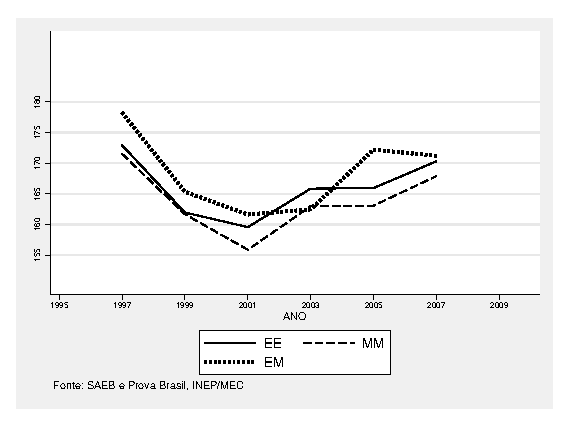
\includegraphics[height=3in]{diff_port}
\end{footnotesize}
\end{figure}
 
%\vspace*{0.5cm} 

%%%%%%%%%%%%%%%%%%%%%%%%%%%%%
%%%%%%%%%%%%%%%%%%%%%%%%%%%%%

%%%%%%%%%%%%%%%%%%%%%%%%%%%%%
%%%%%%%%%%%%%%%%%%%%%%%%%%%%%

%\vspace*{1cm} 

\begin{figure}[h]
\centering
\begin{footnotesize}
\caption{Proficincias mŽdias em matem‡tica por grupo \newline de escolas: SAEB (1997-2005) e Prova Brasil (2007)} 
\label{fig:diff_mat}                             
 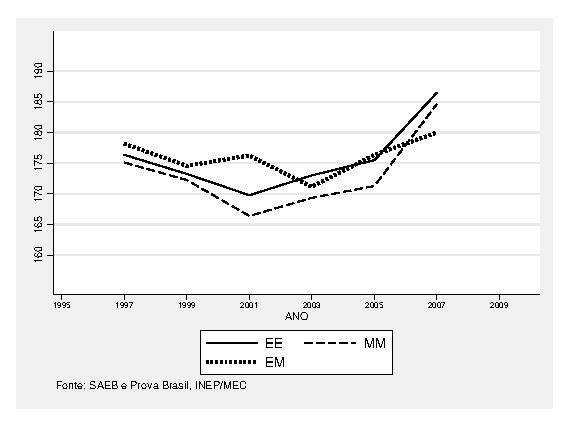
\includegraphics[height=3in]{diff_mat}
\end{footnotesize}
\end{figure}
 
%\vspace*{0.5cm} 

%%%%%%%%%%%%%%%%%%%%%%%%%%%%%
%%%%%%%%%%%%%%%%%%%%%%%%%%%%%


As figuras \ref{fig:diff_port} e \ref{fig:diff_mat} apresentam a exposi‹o visual do comportamento das proficincias mŽdias, em portugus e matem‡tica, segundo o grupo de escolas e o ano,  para o per’odo de 1997 ˆ 2007. Como pode ser observado, as diferenas entre os grupos s‹o muito diminutas para quase todos os anos, tanto em portugus como em matem‡tica. Para alguns anos, em particular, as diferenas entre as proficincias mŽdias parecem aumentar. Como, por exemplo, para o ano de 2001 em matem‡tica ou 2005 em portugus, quando (em ambos os casos) as escolas do grupo tratamento (EM) tiveram um desempenho notavelmente superior aos grupos controle. Contudo, quando se analisa, o tendncia ao longo de todo per’odo, de fato, os grupos tratamento e controle parecem n‹o diferir muito entre si. 

Entretanto, antes de proceder a uma an‡lise mais pormenorizada das proficincias mŽdias dos grupos de escolas, faz-se necess‡rio assegurar que n‹o h‡ grandes disparidades nas caracter’sticas dos alunos e do ambiente familiar entre os grupos tratamento e controle. Pois, como visto anteriormente, pode ser que desvios nas caracter’sticas que podem perturbar o aprendizado dos alunos estejam enviesando os resultados acadmicos dos grupos de escolas. De tal sorte que, inicialmente Ž levada a efeito uma compara‹o das caracter’sticas dos alunos e do ambiente familiar, que podem perturbar o desempenho mŽdio dos grupos de escolas.

%%%%%%%%%%%%%%%%%%%%%%%%%%%%%
%%%%%%%%%%%%%%%%%%%%%%%%%%%%%


\vspace*{1cm}
\begin{table}[htbp]\centering
\begin{footnotesize}
\def\sym#1{\ifmmode^{#1}\else\(^{#1}\)\fi}
\caption{Perfil m�dio dos alunos por grupo de escolas, (1997-2001) \label{tab:diff1997}}
\begin{tabular}{l*{10}{c}}
\toprule
              &\multicolumn{1}{c}{(1997)}&\multicolumn{1}{c}{(1997)}&\multicolumn{1}{c}{(1997)}&\multicolumn{1}{c}{(1999)}&\multicolumn{1}{c}{(1999)}&\multicolumn{1}{c}{(1999)} &\multicolumn{1}{c}{(2001)}&\multicolumn{1}{c}{(2001)}&\multicolumn{1}{c}{(2001)} \\
              &\multicolumn{1}{c}{EE}&\multicolumn{1}{c}{MM}&\multicolumn{1}{c}{EM} &\multicolumn{1}{c}{EE}&\multicolumn{1}{c}{MM}&\multicolumn{1}{c}{EM} &\multicolumn{1}{c}{EE}&\multicolumn{1}{c}{MM}&\multicolumn{1}{c}{EM} \\
               
\midrule
Homens &          49,41\% &    48,61\%&    45,35\% &50,37\% &    50,60\%&    50,25\%&50,68\% &    50,61\%&    49,41\%  \\
%\addlinespace
11 anos &      22,35\%&    21,85\%&    20,71\%&20,21\% &    20,18\%&    20,72\%&23,92\% &    24,50\%&    22,14\%  \\
%\addlinespace
12 anos ou + &      36,81\%&    42,56\%&    28,99\%&35,95\% &    41,65\%&    34,19\%&30,51\% &    33,27\%&    25,89\% \\
%\addlinespace
Branco  &           40,73\%    &    40,78\% &    31,49\%& 41,94\% &    40,54\%&    38,14\% &41,14\% &    39,20\%&    41,45\%   \\
%\addlinespace
Negro &               11,43\% &       9,74\% &      8,28\%& 11,23\% &    12,92\%&    12,88\%&12,78\% &    13,93\%&    15,20\% \\
%\addlinespace
M�e (EM)          &        14,30\% &  10,51\%   & 12,22\%&  7,92\% &    6,45\%&    6,70\%&14,14\% &    12,59\%&    15,38\% \\
%\addlinespace
M�e (sup.) &          5,48\%&    3,93\% &    4,44\%&7,90\% &    5,69\%&    3,10\%&5,38\% &  4,35\%&    5,90\% \\
%\addlinespace
\midrule
\(N\)     &   4.898         &   4.898        &   4.898 &   6.320         &   6.320        &   6.320 &   18.578         &   18.578        &   18.578    \\
\bottomrule
\multicolumn{10}{l}{\footnotesize Fonte: Calculos pr�prios a partir de dados do SAEB/INEP}\\
\multicolumn{10}{l}{\footnotesize Notas: EE: escolas estaduais que permaneceram estaduais }\\
\multicolumn{10}{l}{\footnotesize  MM: escolas municipais que permaneceram municipais}\\
\multicolumn{10}{l}{\footnotesize  EM: escolas estaduais que migraram para as redes municipais}\\
\end{tabular}
\end{footnotesize}
\end{table}

\begin{table}[htbp]\centering
\begin{footnotesize}
\def\sym#1{\ifmmode^{#1}\else\(^{#1}\)\fi}
\caption{Perfil m�dio dos alunos por grupo de escolas, (2003-2007) \label{tab:diff2003}}
\begin{tabular}{l*{10}{c}}
\toprule
              &\multicolumn{1}{c}{(2003)}&\multicolumn{1}{c}{(2003)}&\multicolumn{1}{c}{(2003)}&\multicolumn{1}{c}{(2005)}&\multicolumn{1}{c}{(2005)}&\multicolumn{1}{c}{(2005)} &\multicolumn{1}{c}{(2007)}&\multicolumn{1}{c}{(2007)}&\multicolumn{1}{c}{(2007)} \\
              &\multicolumn{1}{c}{EE}&\multicolumn{1}{c}{MM}&\multicolumn{1}{c}{EM} &\multicolumn{1}{c}{EE}&\multicolumn{1}{c}{MM}&\multicolumn{1}{c}{EM} &\multicolumn{1}{c}{EE}&\multicolumn{1}{c}{MM}&\multicolumn{1}{c}{EM} \\
               
\midrule
Homens &   50,46\% &    50,30\%&    48,08\% & 49,58\% & 49,50\%&  46,37\% & 50,14\% & 50,67\%& 47,27\%  \\
%\addlinespace
11 anos &  23,64\% &    26,22\%&    25,05\% & 25,85\% & 28,31\%&  28,36\% & 23,45\% & 25,99\%& 26,03\%  \\
%\addlinespace
12 anos ou + & 25,41\% &    27,52\%&    18,96\% & 22,85\% & 23,85\%&  12,10\% & 20,27\% & 20,51\%& 13,23\%\\
%\addlinespace
Branco  &  36,01\% &    35,57\%&    34,68\% & 31,92\% & 29,94\%&  25.96\% & 35,63\% & 32,10\%& 38,07\% \\
%\addlinespace
Negro & 11,39\% &    12,11\%&    14,18\% & 12,62\% & 14,11\%&  15,97\% & 12,46\% & 13,39\%& 14,11\% \\
%\addlinespace
M�e (EM) & 13,86\% &    10,81\%&    15,05\% & 13,58\% & 12,48\%&  12,19\% & 15,29\% & 14,23\%& 15,76\% \\
%\addlinespace
M�e (sup.) &  11,96\% &    9,24\%&    6,96\% & 13,32\% & 10,61\%&  11,38\% & 12,59\% & 11,39\%& 10,62\%  \\
%\addlinespace
\midrule
\(N\)     &   16.300         &   16.300        &   16.300 &   17.714         &   17.714        &   17.714 &   58.351         &   58.351        &   58.351    \\
\bottomrule
\multicolumn{10}{l}{\footnotesize Fonte: Calculos pr�prios a partir de dados do SAEB/INEP}\\
\multicolumn{10}{l}{\footnotesize Notas: EE: escolas estaduais que permaneceram estaduais }\\
\multicolumn{10}{l}{\footnotesize  MM: escolas municipais que permaneceram municipais}\\
\multicolumn{10}{l}{\footnotesize  EM: escolas estaduais que migraram para as redes municipais}\\
\end{tabular}
\end{footnotesize}
\end{table}



                             
%%%%%%%%%%%%%%%%%%%%%%%%%%%%%
%%%%%%%%%%%%%%%%%%%%%%%%%%%%%

As tabelas \ref{tab:diff1997} e \ref{tab:diff2003}  apresentam os valores mŽdios para as principais caracter’sticas dos alunos e do ambiente familiar, segundo o grupo de escolas e os anos. Nota-se que, em geral, os grupos s‹o semelhantes, tanto na composi‹o do alunato com rela‹o a idade, gnero e cor, como tambŽm no que se refere ˆ educa‹o da m‹e. Contudo, h‡ pequenos, porŽm consistentes, desvios que merecem ser comentados. 

O mais claro desses desvios na composi‹o do alunato entre os grupos tratamento e controle refere-se a prevalncia de alunos matriculados fora da sŽrie recomendada para sua idade nas escolas do grupo MM e, em menor propor‹o, nas escolas do grupo EM. Percebe-se que, tanto as escolas que permaneceram sob controle dos munic’pios, o grupo MM, como as escolas que foram transferidas, o grupo EM, apresentam maior prevalncia de alunos em situa‹o de atraso escolar. Essa disparidade d‡-se tanto para a categoria \emph{11 anos} -- que representa um atraso escolar de pelo menos dois anos -- e tambŽm para a categoria \emph{12 anos ou mais} -- atraso de pelo menos 3 anos --, nesta œltima, ainda com mais intensidade. TambŽm Ž not‡vel que a distor‹o idade-sŽrie perde fora nos anos finais da sŽrie temporal. Ou seja, percebe-se que a partir de meados dos anos 2000 a prevalncia de alunos matriculados fora da sŽrie recomendada para sua idade tem um decrŽscimo significativo para todos os grupos. Assim, por exemplo, os alunos com 12 anos de idade ou mais matriculados na 4a sŽrie do ensino fundamental nas escolas do grupo MM, que chegaram a representar mais de 42 por cento do total de alunos matriculados nesse grupo de escolas em 1997; paulatinamente, tm sua propor‹o reduzida para pouco mais de 20 por cento do total de alunos das escolas do grupo MM.

A composi‹o racial do alunato entre os grupos tratamento e controle merece um breve coment‡rio. Pois, percebe-se que, ($i$) h‡ um aumento consider‡vel de alunos que se declaram negros nas escolas do grupo tratamento ao longo da sŽrie temporal analisada. A presena de alunos que se declaram negros nas escolas que foram transferidas dos estados para os munic’pios somava pouco menos de 8,5 por cento do total de alunos em 1997. Em 2005, a presena desses alunos praticamente dobra, atingindo pouco menos de 16 por cento do total de alunos matriculados nas escolas do grupo EM. Por outro lado, nota-se que, ($ii$) h‡ um decrŽscimo na propor‹o de alunos que se declaram brancos, a partir de 2003, para todos os grupos de escolas. Esse decrŽscimo Ž, contudo, mais saliente nas escolas dos grupos MM e EM. 

Quando se examina o n’vel de escolaridade da m‹e, observa-se que a porcentagem de m‹es com ensino mŽdio ou superior Ž sempre maior nas escolas do grupo EE, o grupo que permaneceu sobre o controle dos estados, exceto para 1999, quando se nota uma descontinuidade na sŽrie hist—rica. 

Vale destacar que os desvios verificados na composi‹o do corpo discente nos grupos de escolas no per’odo prŽ-municipaliza‹o (1997-2005), em geral, se mantŽm para o per’odo p—s-municipaliza‹o (2007).\footnote{Como j‡ observado no cap’tulo quarto deste estudo, na se‹o metodol—gica, o efeito estimado da municipaliza‹o das escolas n‹o leva em conta o tempo em que as escolas do grupo de tratamento (EM) estiveram sob controle dos munic’pios. Ou seja, a an‡lise ignora o tempo de exposi‹o ˆ gest‹o municipal. Assim, consideram-se aqui apenas dois per’odos: um per’odo inicial, ou per’odo prŽ-municipaliza‹o, que abrange os anos de 1997 a 2005; e um per’odo final, ou p—s-municipaliza‹o, que abrange dos dados da Prova Brasil de 2007.} Salvo pela maior presena de alunos n‹o brancos, que se d‡ em todos os grupos de escolas (embora com mais intensidade nas escolas do grupo tratamento) e pela diminui‹o na propor‹o de alunos matriculados fora da sŽrie recomendada para sua idade, que tambŽm ocorre para todos os grupos de escolas. 

As tabelas \ref{tab:diff1997} e \ref{tab:diff2003}, quando vistas como um pano de fundo para as figuras \ref{fig:diff_port} e \ref{fig:diff_mat}, que mostram a evolu‹o das proficincias mŽdias dos grupos tratamento e controle, oferecem um quadro geral dos alunos e dos grupos de escolas. Esse panorama geral torna evidente, n‹o obstante os desvios mencionados na composi‹o do alunato entre os grupos tratamento e controle, um retrato de alunos e grupos muito semelhantes entre si, tanto em termos de desempenho acadmico como no perfil socioecon™mico. 

Finalmente, antes de proceder  ˆ compara‹o das diferenas em desempenho nas proficincias mŽdias dos grupos tratamento e controle, cabe uma œltima investiga‹o acerca da distribui‹o geogr‡fica dos grupos de escolas nas regi›es do Brasil. Uma vez que, h‡ um diferencial de desempenho entre as regi›es, disparidades na distribui‹o geogr‡fica entre os grupos poderia perturbar a compara‹o nas diferenas de desempenho entre os grupos controle e tratameto.

Leme, Paredes e Souza (2009), j‡ demonstraram que a transferncia de escolas das redes pœblicas estaduais para as redes pœblicas municipais foi mais frequente nas regi›es nordeste e sudeste do pa’s. Os dados apresentados na tabela \ref{tab:regiao}, confirmam os achados daquele estudo.

%%%%%%%%%%%%%%%%%%%%%%%%%%%%%
%%%%%%%%%%%%%%%%%%%%%%%%%%%%%

%\vspace*{0.2cm}
\begin{table}[htbp]\centering
\begin{footnotesize}
\def\sym#1{\ifmmode^{#1}\else\(^{#1}\)\fi}
\caption{Distribui��o dos grupos tratamento e controle  
\newline segundo as regi�es do Brasil \label{tab:regiao}}
\begin{tabular}{l*{4}{c}}
\toprule
              \bf{Regi�o} &  \bf{Grupo EE}& \bf{Grupo MM} & \bf{Grupo EM} \\
              \bf{geogr�fica} & \bf{(Controle I)} & \bf{(Controle II)} &\bf{(Tratamento)} \\
               
\midrule
Norte &   24,38\% &    18,81\%&    09,56\%   \\
%\addlinespace
Nordeste &  31,74\% &    40,61\%&    41,07\%\\
%\addlinespace
Sudeste & 14,27\% &    15,65\%&    29,52\%  \\
%\addlinespace
Sul  &  15,01\% &    15,33\%&    17,15\% \\
%\addlinespace
Centro Oeste & 14,60\% &    09,61\%&    02,70\% \\
%\addlinespace
\midrule
\bottomrule
\multicolumn{4}{l}{\footnotesize Fonte: Calculos pr�prios a partir de dados do SAEB/INEP}\\
\multicolumn{4}{l}{\footnotesize Notas: EE: escolas estaduais que permaneceram estaduais }\\
\multicolumn{4}{l}{\footnotesize  MM: escolas municipais que permaneceram municipais}\\
\multicolumn{4}{l}{\footnotesize  EM: escolas estaduais que migraram para as redes municipais}\\
\end{tabular}
\end{footnotesize}
\end{table}

                             
%%%%%%%%%%%%%%%%%%%%%%%%%%%%%
%%%%%%%%%%%%%%%%%%%%%%%%%%%%%

A tabela \ref{tab:regiao} apresenta a distribui‹o regional dos grupos tratamento e controle. O exame da tabela  \ref{tab:regiao} torna evidente a maior concentra‹o do grupo tratamento nas regi›es nordeste e sudeste, tal como em Leme, Paredes e Souza (2010). O grupo MM, das escolas municipais que permaneceram municipais, tambŽm exibe maior concentra‹o no nordeste. Essa distribui‹o desigual do grupo MM j‡ era esperada e deve-se a maior cobertura das redes municipais, se comparadas ˆs estaduais, na regi‹o nordeste do Brasil (MEC/INEP, 2010). 


Feita a an‡lise da composi‹o socioecon™mica e da distribui‹o geogr‡fica dos grupos tratamento e controle, cujo intuito Ž simplesmente assegurar que os grupos s‹o, de fato, semelhantes o bastante para que sua compara‹o faa sentido; pode-se, agora, avanar a um exame mais detido das diferenas em desempenho acadmico entre os grupos de escolas. Como mencionado anteriormente, a estima‹o por diferena-em-diferenas funda-se, \emph{grosso modo}, na compara‹o das proficincias mŽdias dos grupos tratamento e controle nos per’odos prŽ municipaliza‹o e p—s municipaliza‹o.

Entretanto, Ž importante esclarecer que a estima‹o por diferena-em-diferenas n‹o se trata simplesmente de um teste de compara‹o de proficincias mŽdias n‹o condicionais. Ou seja, n‹o se trata de simplesmente comparar as proficincias mŽdias das escolas sem controlar as demais caracter’sticas dos alunos e do ambiente familiar que podem contribuir para o aprendizado dos estudantes. Mas, pelo contr‡rio, a estima‹o por diferena-em-diferenas -- como outras tŽcnicas de an‡lise de dados em painel --  garante n‹o apenas que se controle as caracter’sticas observadas dos alunos que variam ao longo do tempo, tais como, cor, gnero, idade, entre outras, como tambŽm permite, via o emprego de um termo de efeito espec’fico para as escolas, que se controle as caracter’sticas n‹o observadas das escolas que n‹o variam no tempo. 

Para estimar do efeito da municipaliza‹o sobre a proficincia mŽdia dos grupos tratamento e controle, se ajustou um modelo estat’stico dado pela equa‹o \ref{eq:equac2}. Esse modelo busca captar efeito da municipaliza‹o sobre a proficincia mŽdia das escolas do grupo tratamento (o grupo EM), quando comparadas ˆs escolas dos grupos controle (grupos EE e MM). Cabe destacar ainda, que a estima‹o por diferena-em-diferenas Ž conduzida comparando-se, separadamente, dois grupos de casa vez. Ou seja, inicialmente, compara-se o grupo tratamento com um dos grupos controle, como, por exemplo, com o grupo EE. Ent‹o, num segundo momento, compara-se o grupo tratamento com o grupo controle remanescente, o grupo MM. 

As tabelas \ref{tab:diff3}, \ref{tab:diff4}, \ref{tab:diff} e \ref{tab:diff2} apresentam os resultados da estima‹o por diferena-em-diferenas, com efeito fixo da escola, para os exames de portugus e matem‡tica dos alunos da 4a. sŽrie do ensino fundamental. Os resultados da estima‹o s‹o exibidos separadamente segundo a disciplina, se portugus ou matem‡tica e segundo o grupo controle utilizado, se grupo EE ou grupo MM. 


%%%%%%%%%%%%%%%%%%%%%%%%%%%%%
%%%%%%%%%%%%%%%%%%%%%%%%%%%%%

%\vspace*{0.5cm}
\begin{table}[htbp]\centering
\begin{footnotesize}
\def\sym#1{\ifmmode^{#1}\else\(^{#1}\)\fi}
\caption{Resultados do estimador de diferen�a-em-diferen�as \newline com efeito fixo da escola para portugu�s, 4a. s�rie \label{tab:diff3}}
\begin{tabular}{l*{4}{c}}
\toprule
              \bf{} &  \bf{Grupo EE}& &\bf{Grupo EM}  \\
              \bf{} & \bf{(Controle I)} & &\bf{(Tratamento)}  \\
               
\midrule
Pr� Municipaliza��o   & 164.16(a)  & & 164.24(b)    \\
                                        & (0.39)    & & (2.25)   \\
P�s Municipaliza��o  &   170.31(c) & & 169.43(d)  \\
                                        & (0.41)    & & (2.15)   \\
Diferen�a                      &    0.079(b-a)     & &  -0.88(d-c)  \\
                                       & (2.91)    & & (1.97)   \\
Dif. em Dif.                     & &           \bf{-0.96} &  \\
                                       &    &         \bf{(3.02)} &   \\

\midrule
Controles p/ escolas & & sim &    \\
Controles p/ ano   & & sim &   \\
\(N\)     &                   &   4.734       &     \\   
\(R^2\)     &               &   0.022     &     \\   
\bottomrule
\multicolumn{4}{l}{\footnotesize Erros padr�o ajustados em par�nteses}\\
\multicolumn{4}{l}{\footnotesize \sym{*} \(p<0.05\), \sym{**} \(p<0.01\), \sym{***} \(p<0.001\)}\\
\multicolumn{4}{l}{\footnotesize M�dias e erros padr�o calculados via MQO}\\
\multicolumn{4}{l}{\footnotesize Fonte: C�lculos pr�prios a partir de dados do SAEB e Prova Brasil}\\
\multicolumn{4}{l}{\footnotesize Notas: EE: escolas estaduais que permaneceram estaduais }\\
\multicolumn{4}{l}{\footnotesize  EM: escolas estaduais que migraram para as redes municipais}\\
\end{tabular}
\end{footnotesize}
\end{table}

                             
%%%%%%%%%%%%%%%%%%%%%%%%%%%%%
%%%%%%%%%%%%%%%%%%%%%%%%%%%%%


Pode-se notar, na tabela  \ref{tab:diff3}, que as escolas do grupo EM, no per’odo prŽ municipaliza‹o, tinham uma proficincia mŽdia em portugus, condicional ˆs caracter’sticas observadas dos aluno e ao efeito fixo da escola, de $164,24$ pontos na escala de proficincia do SAEB. As escolas do grupo EE, por sua vez, tinham uma proficincia mŽdia condicional de $164,16$. Depois de municipalizadas, as escolas do grupo EM tiveram uma proficincia mŽdia condicional de $169,43$. Um acrŽscimo de $5,19$ pontos na escala de proficincia em l’ngua portuguesa. Esse incremento na nota mŽdia das escolas do grupo tratamento pode ser atribu’do ˆ municipaliza‹o, como, alternativamente, pode ser atribu’do a uma sŽrie de outros fatores que contribuem para o aprendizado dos alunos. O contrafactual, por conseguinte, seria o que teria acontecido com essas escolas caso tivessem permanecido sob o controle do estado. Isto Ž, caso n‹o tivessem sido municipalizadas. Nesse caso, esperar-se-ia um incremento na proficincia mŽdia das escolas igual aquele experimentado pelas escolas que eram estaduais e que n‹o foram municipalizadas. Isto Ž, um incremento igual ao apresentado pelo grupo controle, que foi de $6,15$,  atingindo $170,31$ pontos na escala SAEB em 2007.

O estimador de diferena-em-diferenas compara a diferena na proficincia mŽdia condicional entre os grupos EM e EE, no per’odo prŽ municipaliza‹o, que Ž igual a $0.079$; com a diferena na proficincia mŽdia condicional, no per’odo p—s municipaliza‹o, que Ž igual a $-0,88$. Calculando-se a diferena das diferenas chega-se ao exato valor do estimador de diferena-em-diferenas, que Ž igual a $-0.96$; ou seja,  $(-0,88)$ - $(0,079)$. Portanto, o efeito da municipaliza‹o Ž igual ao estimador de diferena-em-diferenas; pois, este representa o exato valor da diferena entre o incremento na proficincia mŽdia condicional das escolas estaduais que foram municipalizadas ($5,19$) e o incremento na proficincia mŽdia das escolas estaduais que permaneceram estaduais ($6,15$); isto Ž, $5,19$ - $6,15$ =  -$0,96$. Nesse sentido, cabe destacar que o efeito da municipaliza‹o sobre a proficincia mŽdia condicional Ž quase nulo e n‹o significante estatisticamente. 


%%%%%%%%%%%%%%%%%%%%%%%%%%%%%
%%%%%%%%%%%%%%%%%%%%%%%%%%%%%

%\vspace*{0.5cm}
\begin{table}[htbp]\centering
\begin{footnotesize}
\def\sym#1{\ifmmode^{#1}\else\(^{#1}\)\fi}
\caption{Resultados do estimador de diferen�a-em-diferen�as \newline com efeito fixo da escola para portugu�s, 4a. s�rie \label{tab:diff4}}
\begin{tabular}{l*{4}{c}}
\toprule
              \bf{} &  \bf{Grupo MM}& &\bf{Grupo EM}  \\
              \bf{} & \bf{(Controle II)} & &\bf{(Tratamento)}  \\
               
\midrule
Pr� Municipaliza��o   & 161.39(a)  & & 165.41(b)    \\
                                        & (0.36)    & & (1.90)   \\
P�s Municipaliza��o  &   167.80(c) & & 171.22(d)  \\
                                        & (0.35)    & & (1.84)   \\
Diferen�a                      &    4.01\sym{**}(b-a)     & &  3.41\sym{*}(d-c)  \\
                                       & (0.03)    & & (1.87)   \\
Dif. em Dif.                     & &           \bf{-0.60} &  \\
                                       &    &         \bf{(2.70)} &   \\

\midrule
Controles p/ escolas & & sim &    \\
Controles p/ ano   & & sim &   \\
\(N\)     &                   &   5.767       &     \\   
\(R^2\)     &               &   0.026     &     \\   
\bottomrule
\multicolumn{4}{l}{\footnotesize Erros padr�o ajustados em par�nteses}\\
\multicolumn{4}{l}{\footnotesize \sym{*} \(p<0.05\), \sym{**} \(p<0.01\), \sym{***} \(p<0.001\)}\\
\multicolumn{4}{l}{\footnotesize M�dias e erros padr�o calculados via MQO}\\
\multicolumn{4}{l}{\footnotesize Fonte: C�lculos pr�prios a partir de dados do SAEB e Prova Brasil}\\
\multicolumn{4}{l}{\footnotesize Notas: MM: escolas municipais que permaneceram municipais}\\
\multicolumn{4}{l}{\footnotesize  EM: escolas estaduais que migraram para as redes municipais}\\
\end{tabular}
\end{footnotesize}
\end{table}

                             
%%%%%%%%%%%%%%%%%%%%%%%%%%%%%
%%%%%%%%%%%%%%%%%%%%%%%%%%%%%

A tabela \ref{tab:diff4} apresenta as proficincias mŽdias condicionais dos exames em l’ngua portuguesa dos alunos da 4a. sŽrie do ensino fundamental. Agora, se lana m‹o do grupo de escolas municipais que permaneceram municipais como grupo controle, o grupo MM. Admite-se que a compara‹o entre os grupos MM e EM n‹o Ž t‹o informativa do ponto de vista te—rico como a compara‹o prŽvia, entre os grupos EE e EM; pois, na presente compara‹o o contrafactual seria n‹o o que teria acontecido com as escolas caso tivessem permanecido sob o controle do estado, mas, pelo contr‡rio, o que teria acontecido com as escolas caso estivessem sob o controle dos munic’pios. Entretanto, de um ponto de vista estritamente anal’tico, a compara‹o Ž v‡lida; j‡ que informativa acerca das mudanas nas proficincias mŽdias condicionais dos grupos de escolas que permaneceram municipais e que foram municipalizadas. Ou seja, a compara‹o entre os grupos MM e EM tem a capacidade de informar se houve uma convergncia nas proficincias mŽdias condicionais dos dois grupos ap—s a municipaliza‹o ou se, pelo contr‡rio, a diferena entre as notas mŽdias condicionais tornou-se mais dilatada no per’odo p—s municipaliza‹o.

Feita esta ressalva, o exame da tabela \ref{tab:diff4} demonstra que, no per’odo prŽ municipaliza‹o, as proficincias mŽdias condicionais eram de $161,39$ pontos na escala de proficincia do SAEB para as escolas do grupo MM e $165,41$ pontos para as escolas o grupo EM. Ou seja, a diferena prŽ-municipaliza‹o era de $4,01$ pontos na escala SAEB. Essa diferena era estatisticamente significante ao n’vel de 5 por cento. No per’odo p—s municipaliza‹o, as notas mŽdias condicionais dos grupos MM e EM atingem $167,80$ e $171,22$ pontos, respectivamente. Consequentemente, a diferena nas proficincias mŽdias tem um pequeno decrŽscimo chegando a $3,41$ pontos na escala SAEB. Essa diferena permanece significante, mas ao n’vel de 10 por cento. Portanto, o efeito da municipaliza‹o sobre as escolas transferidas dos estados para os munic’pios, quando comparadas ˆs escolas que j‡ eram municipais e permaneceram municipais Ž de $-0.60$ pontos na escala de proficincia em l’ngua portuguesa. Ou seja, o efeito da municipaliza‹o Ž praticamente nulo e n‹o estatisticamente diferente de zero, isto Ž, n‹o siginificante estatisticamente.

%%%%%%%%%%%%%%%%%%%%%%%%%%%%%
%%%%%%%%%%%%%%%%%%%%%%%%%%%%%

%\vspace*{0.5cm}
\begin{table}[htbp]\centering
\begin{footnotesize}
\def\sym#1{\ifmmode^{#1}\else\(^{#1}\)\fi}
\caption{Resultados do estimador de diferen�a-em-diferen�as \newline com efeito fixo da escola para matem�tica, 4a. s�rie \label{tab:diff}}
\begin{tabular}{l*{4}{c}}
\toprule
              \bf{} &  \bf{Grupo EE}& &\bf{Grupo EM}  \\
              \bf{} & \bf{(Controle I)} & &\bf{(Tratamento)}  \\
               
\midrule
Pr� Municipaliza��o   & 173.14(a)  & & 174.62(b)    \\
                                        & (0.39)    & & (2.21)   \\
P�s Municipaliza��o  &   186.50(c) & & 186.01(d)  \\
                                        & (0.43)    & & (2.15)   \\
Diferen�a                      &    1.48(b-a)     & &  -0.48(d-c)  \\
                                       & (2.25)    & & (2.20)   \\
Dif. em Dif.                     & &           \bf{-1.96} &  \\
                                       &    &         \bf{(3.15)} &   \\

\midrule
Controles p/ escolas & & sim &    \\
Controles p/ ano   & & sim &   \\
\(N\)     &                   &   4.733       &     \\   
\(R^2\)     &               &   0.095     &     \\   
\bottomrule
\multicolumn{4}{l}{\footnotesize Erros padr�o ajustados em par�nteses}\\
\multicolumn{4}{l}{\footnotesize \sym{*} \(p<0.05\), \sym{**} \(p<0.01\), \sym{***} \(p<0.001\)}\\
\multicolumn{4}{l}{\footnotesize M�dias e erros padr�o calculados via MQO}\\
\multicolumn{4}{l}{\footnotesize Fonte: C�lculos pr�prios a partir de dados do SAEB e Prova Brasil}\\
\multicolumn{4}{l}{\footnotesize Notas: EE: escolas estaduais que permaneceram estaduais }\\
\multicolumn{4}{l}{\footnotesize  EM: escolas estaduais que migraram para as redes municipais}\\
\end{tabular}
\end{footnotesize}
\end{table}

                             
%%%%%%%%%%%%%%%%%%%%%%%%%%%%%
%%%%%%%%%%%%%%%%%%%%%%%%%%%%%

As tabelas \ref{tab:diff} e \ref{tab:diff2} apresentam os resultados da estima‹o do efeito da municipaliza‹o sobre as proficincias nos exames em matem‡tica para os alunos da 4a. sŽrie do ensino fundamental. Primeiramente, deve-se notar que os resutlados para os exames em matem‡tica pouco diferem daqueles apresentados acerca dos exames em l’ngua portuguesa. 

A tabela \ref{tab:diff} traz a compara‹o entre os grupos EE e EM, a mais informativa do ponto de vista te—rico, pois aquela que tem a capacidade de instruir acerca do efeito da municipaliza‹o na proficincia mŽdia das escolas municipalizadas (EM), quando comparadas ˆs escolas que permaneceram sob o controle dos estados (EE). O exame da dos estimadores reportados na tabela \ref{tab:diff} mostram que, no per’odo prŽ municipaliza‹o, a proficincia mŽdia condicional do grupo de escolas que foi transferido para os munic’pios era de $174,62$ pontos na escala SAEB. A mŽdia condicional do grupo de escolas que permaneceu sob o controle dos estados era de $173,14$ pontos. Havia, portanto, uma diferena nas proficincias condicionais, prŽ municipaliza‹o, de exatamente $1,48$ pontos. O contrafactual, nesse caso, seria o que teria acontecido com as escolas municipalizadas, caso tivessem permanecido sob o controle dos estados. Sob essa situa‹o hipotŽtica eperar-se-ia que nota mŽdia condicional tivesse um incremento de $13.36$ pontos no per’odo p—s municipaliza‹o, tal como se deu com as escolas do grupo controle que tiveram uma proficincia mŽdia condicional de $186,50$. Nessa situa‹o, a diferena nas proficincias mŽdias condicionais manter-se-ia em, exatamente, $1,48$ pontos e a nota mŽdia condicional das escolas municipalizadas seria de $187,98$. Contudo, a proficincia mŽdia condicional das escolas municipalizadas foi de $186,01$ pontos SAEB, no p—s municipaliza‹o. Isto Ž, o incremento na proficincia mŽdia do grupo tratamento foi de $11,29$ pontos. A diferena p—s-municipaliza‹o entre os grupos controle e tratamento, por conseguinte, foi de $-0.48$ pontos. Logo, pode-se concluir que o efeito da municipaliza‹o, que Ž dado pelo exato valor da diferena entre diferenas, prŽ e p—s municipaliza‹o, nas proficincias mŽdias condicionais, foi de $(-1.96)$ pontos; ou seja, $(-0.48)  - (1,48)$.  Mais uma vez, o efeito estimado da municipaliza‹o Ž n‹o apenas pouco expressivo em termos de sua magnitude, como tambŽm n‹o se pode assegurar que seja estatisticamente diferente de zero.

%%%%%%%%%%%%%%%%%%%%%%%%%%%%%
%%%%%%%%%%%%%%%%%%%%%%%%%%%%%

%\vspace*{0.5cm}

\begin{table}[htbp]\centering
\begin{footnotesize}
\def\sym#1{\ifmmode^{#1}\else\(^{#1}\)\fi}
\caption{Resultados do estimador de diferen�a-em-diferen�as \newline com efeito fixo da escola para matem�tica, 4a. s�rie \label{tab:diff2}}
\begin{tabular}{l*{4}{c}}
\toprule
              \bf{} &  \bf{Grupo MM}& &\bf{Grupo EM}  \\
              \bf{} & \bf{(Controle II)} & &\bf{(Tratamento)}  \\
               
\midrule
Pr� Municipaliza��o   & 170.09(a)  & & 174.80(b)    \\
                                        & (0.35)    & & (1.94)   \\
P�s Municipaliza��o  &   184.64(c) & & 187.40(d)  \\
                                        & (0.43)    & & (2.02)   \\
Diferen�a                      &    4.72\sym{**}(b-a)     & &  2.76(d-c)  \\
                                       & (1.97)    & & (2.06)   \\
Dif. em Dif.                     & &           \bf{-1.95} &  \\
                                       &    &         \bf{(2.85)} &   \\

\midrule
Controles p/ escolas & & sim &    \\
Controles p/ ano   & & sim &   \\
\(N\)     &                   &   5.766       &     \\   
\(R^2\)     &               &   0.114     &     \\   
\bottomrule
\multicolumn{4}{l}{\footnotesize Erros padr�o ajustados em par�nteses}\\
\multicolumn{4}{l}{\footnotesize \sym{*} \(p<0.05\), \sym{**} \(p<0.01\), \sym{***} \(p<0.001\)}\\
\multicolumn{4}{l}{\footnotesize M�dias e erros padr�o calculados via MQO}\\
\multicolumn{4}{l}{\footnotesize Fonte: C�lculos pr�prios a partir de dados do SAEB e Prova Brasil}\\
\multicolumn{4}{l}{\footnotesize Notas: MM: escolas municipais que permaneceram municipais}\\
\multicolumn{4}{l}{\footnotesize  EM: escolas estaduais que migraram para as redes municipais}\\
\end{tabular}
\end{footnotesize}
\end{table}

                             
%%%%%%%%%%%%%%%%%%%%%%%%%%%%%
%%%%%%%%%%%%%%%%%%%%%%%%%%%%%


Finalmente, a tabela \ref{tab:diff2} exibe os resultados da estima‹o na qual s‹o comparadas as proficincias condicionais mŽdias em matem‡tica dos grupos de escolas MM e EM. A an‡lise dos estimadores apresentados nesta tabela apontam que a nota condicional mŽdia do grupo de escolas municipalizadas era, no per’odo prŽ municipaliza‹o, igual a $174,80$ pontos. A proficincia condicional mŽdia do grupo de escolas que permaneceram sob controle municipal era de $170,09$. A diferena nas proficincias mŽdias, prŽ municipaliza‹o era, portanto, igual a $4,72$ pontos na escala de proficincia em matem‡tica. Essa diferena era estatisticamente significante ao n’vel de 5 por cento. Ap—s a municipaliza‹o, verifica-se que a proficincia mŽdia das escolas municipalizadas Ž de $187,40$; ou seja, houve um incremento na proficincia mŽdia desse grupo de escolas de $12,6$ pontos. A proficincia condicional mŽdia do grupo de escolas que permaneceu sob a gest‹o municipal atinge $184,64$ pontos. Isto Ž, houve um incremento de $14,55$ pontos na escala SAEB. A diferena na proficincia condicional mŽdia entre os grupos tratamento e controle, que era de $4,72$ pontos no per’odo prŽ municipaliza‹o, cai para $2,76$ pontos no per’odo p—s municipaliza‹o. Ou seja, nota-se um decrŽscimo de $-1,96$ pontos nas diferenas prŽ e p—s municipaliza‹o. Esse decrŽscimo nas diferenas Ž o efeito da municipaliza‹o sobre as proficincias condicionais mŽdia dos exames em matem‡tica para o grupo de escolas municipalizadas, se comparado ao grupo de escolas que permaneceu sob o controle das redes municipais. Ainda, cabe destacar que esse efeito praticamente nulo e estatisticamente n‹o diferente de zero.  

%%%%%%%%%%%%%%%%%%%%%%%%%%%%%
%%%%%%%%%%%%%%%%%%%%%%%%%%%%%

\vspace*{1cm} 

\begin{figure}[h]
\centering
\begin{footnotesize}
\caption{Distribui‹o da vari‰ncia das proficincias mŽdias condicionais em matem‡tica por grupo de escolas : EM x MM} \label{fig:EMMM}                             
 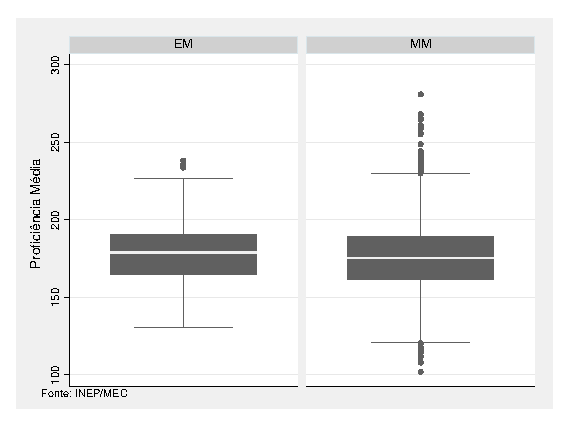
\includegraphics[height=3in]{EMMM}
\end{footnotesize}
\end{figure}
 
%\vspace*{0.5cm} 

%%%%%%%%%%%%%%%%%%%%%%%%%%%%%
%%%%%%%%%%%%%%%%%%%%%%%%%%%%%

%%%%%%%%%%%%%%%%%%%%%%%%%%%%%
%%%%%%%%%%%%%%%%%%%%%%%%%%%%%

%\vspace*{1cm} 

\begin{figure}[h]
\centering
\begin{footnotesize}
\caption{Distribui‹o da vari‰ncia das proficincias mŽdias condicionais em matem‡tica por grupo de escolas: EM x EE} 
\label{fig:EMEE}                             
 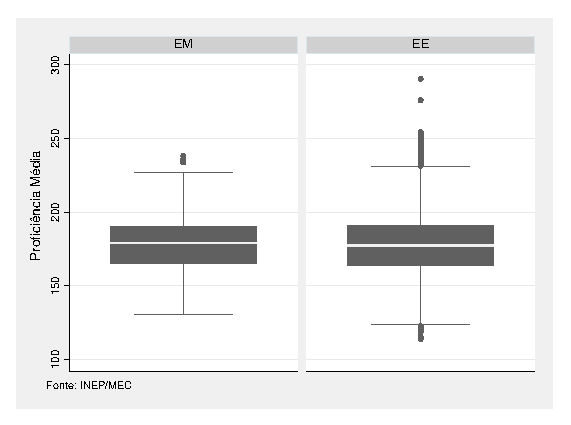
\includegraphics[height=3in]{EMEE}
\end{footnotesize}
\end{figure}
 
%\vspace*{0.5cm} 

%%%%%%%%%%%%%%%%%%%%%%%%%%%%%
%%%%%%%%%%%%%%%%%%%%%%%%%%%%%

O quadro geral exposto pelo conjunto das tabelas \ref{tab:diff3}, \ref{tab:diff4}, \ref{tab:diff} e \ref{tab:diff2} demonstra que n‹o h‡ efeito percept’vel da municipaliza‹o sobre o desempenho mŽdio das escolas nos exames de proficincia conduzidos pelo MEC/INEP, seja em matem‡tica, seja em l’ngua portuguesa. Os estimadores de diferena-em-diferenas apontam que, mesmo depois de controlar pelas caracter’sticas observadas dos alunos e pelas caracter’sticas n‹o observadas das escolas, o efeito da municipaliza‹o sobre a proficincia mŽdia das escolas Ž praticamente nulo e n‹o se mostrou estatisticamente diferente de zero em nenhum dos grupos ou disciplinas.

N‹o obstante o efeito estimado da municipaliza‹o sobre o desempenho acadmico das escolas seja sempre negativo, tanto em matem‡tica como em l’ngua portuguesa, pode-se especular que as mŽdias condicionais s‹o t‹o pr—ximas e as vari‰ncias das proficincias mŽdias entre as escolas dos grupos tratamento e controle s‹o t‹o grandes que a estima‹o por diferena-em-diferenas, via MQO ou EF, n‹o Ž capaz de captar as nuanas de subgrupos de escolas que possivelmente estejam respondendo (positiva ou negativamente, n‹o vem ao caso) ˆ municipaliza‹o. As figuras \ref{fig:EMMM} e \ref{fig:EMEE} exibem a distribui‹o da vari‰ncia das proficincias mŽdias condicionais em matem‡tica segundo os grupos comparados via estima‹o por diferena-em-diferenas. Nota-se que tanto para o grupo tratamento como para os grupos controle, a vari‰ncia das proficincias mŽdias Ž significativamente elevada entre as escolas, tanto em termos de amplitude interquart’lica como tambŽm pela presena de de valores discrepantes. 

A t’tulo de conclus‹o, vale recapitular os principais achados da presente se‹o. Nesta se‹o, ($i$) buscou-se estimar o efeito da municipaliza‹o das escolas sobre a proficincia mŽdia de seus alunos, quando comparados aos alunos das escolas que permaneceram sob gest‹o dos estados ou dos munic’pios. ($ii$) O efeito da municipaliza‹o que se buscou estimar Ž exatamente o efeito mŽdio do grupo de escolas que foram transferidas para o controle dos munic’pios, quando cotejadas ˆs escolas que permaneceram sob o controle das redes estaduais e municipais. ($iii$) O estimador de diferena-em-diferenas evidencia que n‹o h‡ efeito relevante da municipaliza‹o sobre o desempenho mŽdio das escolas nos exames de proficincia do conduzidos pelo MEC/INEP, seja em matem‡tica, seja em l’ngua portuguesa. ($iv$) Pode-se especular que o emprego de controles para as caracter’sticas observadas dos alunos e para as caracter’sticas n‹o observadas das escolas ainda n‹o seja suficiente para isolar o impacto da municipaliza‹o, dada a proximidade das mŽdias condicionais e a distribui‹o da vari‰ncia das proficincias mŽdias.   


%%%%%%%%%%%%%%%%%%%%%%%%%%%%%%%%%
%%%%%%%%%%%%%%%%%%%%%%%%%%%%%%%%%


\pagebreak
\subsection{O Efeito da municipaliza‹o sobre as redes escolares}

Tendo estabelecido, nas prŽvias se›es, que ($i$)  uma vez controladas ˆs caracter’sticas dos alunos, e os fatores escolares que podem perturbar o aprendizado dos estudantes, o efeito da rede escolar sobre a proficincia dos alunos torna-se negligenci‡vel. ($ii$) O impacto da municipaliza‹o das escolas sobre o desempenho acadmico de seus alunos nos exames de proficincia do conduzidos pelo MEC/INEP Ž praticamente nulo.

Nesta se‹o, busca-se examinar se houve efeito relevante da municipaliza‹o de matr’culas sobre a qualidade dos servios educacionais oferecidos nos munic’pios brasileiros. Mais especificamente, procura-se estimar o efeito da taxa de municipaliza‹o das matr’culas sobre alguns indicadores selecionados de insumos escolares e de rendimento do fluxo escolar. Para tanto, utiliza-se uma base de dados em painel na qual as unidades de observa‹o s‹o os munic’pios brasileiros. Essa base de dados compreende 2.837 munic’pios e o per’odo de 1999 a 2005.

Como mencionado na se‹o metodol—gica do cap’tulo quarto desta tese, a medida de descentraliza‹o utilizada, como vari‡vel explicativa, nesta an‡lise Ž a taxa de municipaliza‹o de matr’culas nos munic’pios. Isto Ž, trata-se da propor‹o de matr’culas no ensino fundamental em escolas da rede pœblica municipal em fun‹o do total de matr’culas no ensino fundamental pœblico no munic’pio. A taxa de municipaliza‹o procura captar o esforo do munic’pio em incorporar novas matr’culas no ensino fundamental. Esse esforo pode se realizar tanto por meio da cria‹o de novas vagas em escolas da rede pœblica municipal, como pela municipaliza‹o de escolas do ensino fundamental antes mantidas pelos estados. Deve-se destacar que, quando maior a taxa de municipaliza‹o no munic’pio, mais descentralizada a provis‹o da educa‹o neste munic’pio; pois maior a responsabilidade do munic’pio na oferta de educa‹o pœblica \emph{vis-ˆ-vis} a responsabilidade do estado.

As vari‡veis respostas desta an‡lise est‹o subagrupadas em dois conjuntos de indicadores: ($i$) os insumos escolares e os ($ii$) as taxas de rendimento de fluxo escolar. O primeiro conjunto compreende: indicadores a respeito da infraestrutura f’sica das escolas, como, por exemplo, se as escolas possuem biblioteca, quadra de esportes, laborat—rio de cincias, laborat—rio de inform‡tica, a raz‹o computador por aluno, se a escola oferece merenda aos alunos, entre outros; indicadores acerca da composi‹o e forma‹o do corpo docente, como, por exemplo, raz‹o professor por aluno e propor‹o de professores com curso superior. O segundo conjunto de vari‡veis, referentes ao rendimento do fluxo escolar, inclui: taxa de reprova‹o, taxa de abandono e a taxa de distor‹o idade-sŽrie. As tabelas \ref{tab:varinsumos} e \ref{tab:varendimento}, j‡ apresentadas no cap’tulo quatro da tese na se‹o metodol—gica, traz a rela‹o completa das vari‡veis respostas, bem como suas mŽdias segundo a rede escolar.

Em suma, nesta se‹o busca-se examinar a rela‹o entre o esforo do munic’pio na provis‹o do ensino fundamental pœblico e a qualidade da educa‹o ofertada ˆ popula‹o pelas redes pœblica municipal, pœblica estadual e privada. Como mencionado anteriormente, optou-se pela manuten‹o dos dados referentes ˆ rede privada na base de dados, diferentemente do que se deu nas duas an‡lises prŽvias, pois entende-se que as escolas da rede privada podem agora funcionar como um importante grupo controle; j‡ que supostamente a oferta privada de servios educacionais n‹o foi afetada pela municipaliza‹o das matr’culas. Ademais, como as informa›es das escolas foram agregadas para o n’vel do munic’pio segundo o ano e a rede, se municipal, estadual ou privada, a base de dados permite acompanhar o impacto da expans‹o das matr’culas municipais sobre as redes escolares separadamente. 

A equa‹o \ref{eq:equac15}, apresentada na se‹o metodol—gica do cap’tulo quarto da tese, procura modelar o efeito da taxa de municipaliza‹o das matriculas nos munic’pios sobre os insumos escolares e as taxas de rendimento do fluxo escolar nas redes escolares pœblica municipal, pœblica estadual e privada para o painel de 2.837 munic’pios. 

%%%%%%%%%%%%%%%%%%%%%%%%%%%%%
%%%%%%%%%%%%%%%%%%%%%%%%%%%%%

%\vspace*{0.5cm}
\begin{singlespacing}
\begin{table}[htbp]\centering
\begin{footnotesize}
\def\sym#1{\ifmmode^{#1}\else\(^{#1}\)\fi}
\caption{Efeito da taxa de municipaliza��o sobre os insumos escolares\label{tab:xtreginsumos}}
\begin{tabular}{l*{5}{c}}
\toprule
          &\multicolumn{1}{c}{(1)}&\multicolumn{1}{c}{(2)}&\multicolumn{1}{c}{(3)}&\multicolumn{1}{c}{(3)}\\
          &\multicolumn{1}{c}{(Todas)}&\multicolumn{1}{c}{(Municipais)}&\multicolumn{1}{c}{(Estaduais)}&\multicolumn{1}{c}{(Privadas)}\\
          &\multicolumn{1}{c}{Modelo 14}&\multicolumn{1}{c}{Modelo 15}&\multicolumn{1}{c}{Modelo 16}&\multicolumn{1}{c}{Modelo 17}\\
\midrule
Bibliotecas &    -0.0006         &    -0,0016         &    0.0005 & 0.0002         \\
          &  (0.0003)         &  (0.0022)         &  (0.0010) & (0.0003)        \\
%\addlinespace
Quadra de esportes &      -0.0002            &    -0.0027         &   0.0002 & 0.0003         \\
          &  (0.0042)                &  (0.0051)         &  (0.0230) & (0.0065)         \\
%\addlinespace
Laborat�rio de ci�ncias &       -0.0021           &   -0.0052         & -0.0034 & 0.0001         \\
          &        (0.0703)          &  (0.0028)         &  (0.0082)      & (0.0024)   \\
%\addlinespace
Laborat�rio de inform�tica &     0.0019\sym{*} &    0.0051\sym{**}&  0.0016\sym{*}  & 0.0021  \\
              &  (0.0036)         &  (0.0030) &   (0.0013)   &   (0.0022)       \\
%\addlinespace
Aluno/computador &          0.0001        &    -0.0001 &    0.0002  & 0.0001 \\
          &     (0.0002)             &  (0.0002)         &  (0.0003)  & (0.0015)        \\
%\addlinespace
Aluno/Professor &       -0.0003  &  -0.0011 &    -0.0002 & -0.0000        \\
          &         (0.0001)         &  (0.0034)         &  (0.0017) & (0.0012)        \\
%\addlinespace
Curso superior &  0.0003\sym{*}    &  0.0023\sym{**}    &    0.0015\sym{*}   & 0.0010 \\
          &          (0.0003)        &       (0.0015)           &  (0.0009)    & (0.0097)     \\
%\addlinespace
\midrule
\emph{N}     &     26.086         &     12.698         &    8.051 &  5337         \\
\emph{Grupos}     &     2.837         &     2.837        &     2.837 & 2.837         \\
\emph{Controles p/ munic�pios} &    sim        &    sim        &    sim & sim            \\
\emph{dummy   de ano} &    sim        &    sim        &    sim & sim            \\
\emph{Constante} &    sim        &    sim        &    sim & sim         \\
\bottomrule
\multicolumn{5}{l}{\footnotesize Erros padr�o robustos em par�nteses}\\
\multicolumn{5}{l}{\footnotesize Fonte: Calculos pr�prios a partir de dados do MEC/INEP}\\
\multicolumn{5}{l}{\footnotesize \sym{*} \(p<0.05\), \sym{**} \(p<0.01\), \sym{***} \(p<0.001\)}\\
\end{tabular}
\end{footnotesize}
\end{table}
\end{singlespacing}


                             
%%%%%%%%%%%%%%%%%%%%%%%%%%%%%
%%%%%%%%%%%%%%%%%%%%%%%%%%%%%

A tabela \ref{tab:xtreginsumos} mostra os resultados da estima‹o, pelo mŽtodo de efeitos fixos, do impacto da taxa de municipaliza‹o sobre os insumos escolares nas redes escolares pœblicas municipais e estaduais e na rede privada. Antes de passar ˆ an‡lise dos resultados, vale esclarecer que cada um dos itens apresentados na tabela foram regredidos, um a um, na taxa de municipaliza‹o. Primeiro, para todo o conjunto de escolas, cujos resultados s‹o exibidos na coluna (1) da tabela \ref{tab:xtreginsumos}. Em seguida, apenas para as escolas pœblicas municipais, cujos resultados s‹o reportados na coluna (2); e, assim por diante, para as escolas estaduais e privadas, cujos resultados s‹o reportados nas colunas (3) e (4), respectivamente. Em todos os modelos foram inclu’das as vari‡veis de controle dos munic’pios (listadas na tabela \ref{tab:varcontroles}, do cap’tulo quarto), o termo de efeito espec’fico para o munic’pio e \emph{dummies} para os anos, tal como modelado pela equa‹o \ref{eq:equac15}.

A an‡lise da tabela \ref{tab:xtreginsumos} indica que a taxa de municipaliza‹o de matr’culas do ensino fundamental nos munic’pios tem um efeito global muito tnue sobre os insumos escolares das redes pœblicas de ensino. T‹o somente a propor‹o de escolas equipadas com \emph{laborat—rios de Inform‡tica} nos munic’pios e a propor‹o de professores do ensino fundamental com \emph{curso superior} mostram resultados estatisticamente diferentes de zero.

A propor‹o de escolas do ensino fundamental equipadas com bibliotecas parece n‹o ser afetada pela taxa de municipaliza‹o das matr’culas de ensino fundamental. Os coeficientes estimados s‹o negativos para o conjunto de escolas dos munic’pios e para as escolas das redes municipais, embora estatisticamente n‹o diferentes de zero. Para as escolas pœblicas estaduais e municipais os coeficientes s‹o positivos e n‹o estatisticamente  significantes. Para todas as redes a magnitude dos coeficientes estimados Ž pequena. O coeficiente estimado para a rede municipal, por exemplo, indica que para um aumento de 1 ponto percentual na taxa de municipaliza‹o das matriculas, esperar-se-ia um decrŽscimo de 0.0016 pontos percentuais, em mŽdia,  na propor‹o de escolas municipais equipadas bom bibliotecas no munic’pio. Contundo, mais uma vez, vale lembrar que n‹o se pode assegurar que esse coeficiente n‹o seja estatisticamente diferente de zero, dada a ausncia de signific‰ncia estat’stica da estima‹o. 

A propor‹o de escolas equipadas com quadra de esportes n‹o Ž tampouco impactada pela taxa de municipaliza‹o das matr’culas no munic’pio. Os coeficientes estimados, novamente, s‹o negativos para o conjunto de todas as escolas que oferecem matr’culas no ensino fundamental e para as escolas da rede pœblica municipal. Para as escolas da rede pœblica estadual e da rede privada, os coeficientes estimados s‹o positivos. Nenhum desses coeficientes, no entanto, exibe signific‰ncia estat’stica aos n’veis padr‹o de 1, 5 ou 10 por cento. 

Tal como se d‡ com as bibliotecas e quadra de esportes, o coeficiente estimado para o efeito da taxa de municipaliza‹o sobre a propor‹o de escolas equipadas com laborat—rios de cincias Ž negligenci‡vel. Os coeficientes s‹o negativos para o conjunto global de escolas de munic’pio e para as escolas municipais e estaduais das redes pœblicas. Para a rede privada o coeficiente Ž praticamente nulo. Nenhuma das estima›es exibe signific‰ncia estat’stica. 

O efeito estimado da taxa de municipaliza‹o das matr’culas do ensino fundamental sobre a propor‹o de escolas equipadas com laborat—rios inform‡tica Ž relevante. Um incremento de 1 ponto percentual na taxa de municipaliza‹o das matr’culas do ensino fundamental impacta positivamente a propor‹o de escolas municipais equipadas com laborat—rios de inform‡tica em mŽdia 0.005 pontos percentuais. Esse efeito estimado Ž estatisticamente significante ao n’vel de 5 por cento. O conjunto de todas as escolas (que tm matriculas no ensino fundamental) do munic’pio e as escolas da rede pœblica estadual tambŽm se mostram positivamente afetadas pela taxa de municipaliza‹o, embora o efeito estimado seja menor tanto em termos de magnitude do coeficiente estimado -- de aproximadamente 0.001 pontos percentuais em ambos os casos -- como em rela‹o ao n’vel de signific‰ncia estat’stica do coeficiente, que se mostra n‹o diferente de zero apenas a um n’vel de 10 por cento. 

A raz‹o aluno/professor, como tambŽm a raz‹o aluno/computador, n‹o s‹o afetadas pela taxa de municipaliza‹o das matr’culas. Os coeficientes s‹o todos praticamente nulos para esses itens e n‹o se mostram estatisticamente diferentes de zero. Cabe, entretanto, um pequeno coment‡rio a respeito da ausncia de efeito percept’vel da taxa de municipaliza‹o sobre as raz‹o aluno/professor na rede pœblica municipal. Sabe-se que houve um consider‡vel aumento no nœmero de alunos matriculados em escolas das redes pœblicas municipais no ensino fundamental no per’odo investigado (1999-2005), como demonstrado no terceiro cap’tulo desta tese.  Pode-se especular, portanto, que houve um aumento no nœmero de professores mais que proporcional ao aumento no nœmero de alunos matriculados em escolas municipais de ensino fundamental. Esse achado vai ao encontro de outros trabalhos na ‡rea, como em Franco e Menezes-Filho (2009). O mesmo pode-se argumentar a respeito da raz‹o aluno/computador. Resultado corroborado pelo efeito positivo da taxa de municipaliza‹o na propor‹o de escolas municipais equipadas com laborat—rios de inform‡tica. 

A propor‹o de professores do ensino fundamental com curso superior Ž impactada positivamente pela taxa de municipaliza‹o das matriculas no ensino fundamental. Em escolas das redes pœblicas municipais, por exemplo, um aumento de 1 ponto percentual na taxa de municipaliza‹o tem um impacto positivo mŽdio de 0.0023 na propor‹o de professores com curso superior. O coeficiente estimado Ž significante ao n’vel de 5 por cento. Esse efeito se mostrou tambŽm positivo e significante para as escolas estaduais da rede pœblica e para o conjunto de todas as escolas, n‹o obstante em menor magnitude e com signific‰ncia estat’stica apenas ao n’vel de 10 por cento. ƒ importante observar que n‹o Ž poss’vel decompor o efeito independente da taxa de municipaliza‹o das matr’culas sobre a propor‹o de professores com curso superior do efeito da Lei de Diretrizes e Bases da Educa‹o Nacional (LDB), de 1996, que torna obrigat—rio o n’vel de educa‹o superior (em curso de licenciatura realizado em universidades ou institutos superiores de educa‹o) para os professores da educa‹o b‡sica. 


%%%%%%%%%%%%%%%%%%%%%%%%%%%%%
%%%%%%%%%%%%%%%%%%%%%%%%%%%%%

%\vspace*{0.5cm}
\begin{singlespacing}
\begin{sidewaystable}[htbp]\centering
\begin{footnotesize}
\def\sym#1{\ifmmode^{#1}\else\(^{#1}\)\fi}
\caption{Efeito da taxa de municipaliza��o sobre a taxa de reprova��o\label{tab:xtregreprovacao}}
\begin{tabular}{l*{9}{c}}
\toprule
          &\multicolumn{1}{c}{(1)}&\multicolumn{1}{c}{(2)}&\multicolumn{1}{c}{(3)}&\multicolumn{1}{c}{(4)}&\multicolumn{1}{c}{(5)}&\multicolumn{1}{c}{(6)}&\multicolumn{1}{c}{(7)}&\multicolumn{1}{c}{(8)}\\
          &\multicolumn{1}{c}{Todas}&\multicolumn{1}{c}{Todas}&\multicolumn{1}{c}{Municipais}&\multicolumn{1}{c}{Municipais}&\multicolumn{1}{c}{Estaduais}&\multicolumn{1}{c}{Estaduais}&\multicolumn{1}{c}{Privadas}&\multicolumn{1}{c}{Privadas}\\
          &\multicolumn{1}{c}{Modelo 18}&\multicolumn{1}{c}{Modelo 19}&\multicolumn{1}{c}{Modelo 20}&\multicolumn{1}{c}{Modelo 21}&\multicolumn{1}{c}{Modelo 22}&\multicolumn{1}{c}{Modelo 23}&\multicolumn{1}{c}{Modelo 24}&\multicolumn{1}{c}{Modelo 24}\\
\midrule
Reprova��o &    -0.0029         &    -0,0038         &    -0.0047 & -0.0053 &    -0.0012         &    -0,0018         &    -0.0007 & 0.0000         \\
          &  (0.0053)         &  (0.0062)  &  (0.041) & (0.0063)&  (0.0023)         &  (0.0032)         &  (0.0001) & (0.0003)        \\
%\addlinespace
Bibliotecas &          &    -0,0003  &       &    -0.0017 &  &-0.0007 & & 0.0000       \\
          &         &  (0.0008)         &   & (0.0003)  & & (0.0002) && (0.0005)   \\
%\addlinespace
Quadra de esportes &          &    0,0016  &       &    0.0027 &  &0.0007 & & 0.0000            \\
          &         &  (0.0022)         &  & (0.0023)  & & (0.0002) && (0.0002)    \\
%\addlinespace
Lab. de ci�ncias &          &    -0,0021  &       &    -0.0017 &  &-0.0007 & & 0.0000     \\
          &                &  (0.0022)         &  & (0.0003)  & & (0.0002) && (0.0005)   \\
%\addlinespace
Lab. de inform�tica  &          &    0,0006  &       &    0.0009 &  &0.0003 & & 0.0008      \\
              &             &  (0.0012)         &  & (0.0003)  & & (0.0002) && (0.0005)         \\
%\addlinespace
Aluno/computador &          &    0,0000  &       &    0.0013 &  & 0.0007 & & -0.0004     \\
          &                &  (0.0002)         &  & (0.0003)  & & (0.0003) && (0.0001)         \\
%\addlinespace
Aluno/Professor    &          &    0,0013  &       &    0.0017 &  &0.0007 & & 0.0000         \\
          &               &  (0.0032)         & & (0.0023)  & & (0.0008) && (0.0003)   \\
%\addlinespace
 Curso Superior &          &    -0,0013  &       &    -0.0004 &  &-0.0008 & & 0.0006      \\
          &                  &  (0.0017)         &  & (0.0003)  & & (0.0002) && (0.0005)    \\
%\addlinespace
%\addlinespace
Constante    &    6.500\sym{***}&    6.503\sym{***}& 4.515\sym{***}&4.523\sym{***}&    5.303\sym{***}&    5.5206\sym{***}&14.515\sym{***}&14.856\sym{***}\\
          &  (0.1503)         &  (0.1503)         &  (0.1887)&  (0.1898)         &  (0.2687)         &  (0.2700)   &  (0.1030)         &  (0.1032)   \\

\midrule
\emph{N}     &     26.084  &     26.075        &     12.698    &     12.696 &    8.048&    8.048 &  5337  &  5337    \\
\(R^{2} within\) & 0.0002            &    0.017         &    0.073  & 0.0002            &    0.017         &    0.073  & 0.0002            &    0.017        \\
\(R^{2} Between\) &    0.0159         &    0.310         &    0.195  & 0.0002            &    0.017         &    0.073  & 0.0002            &    0.017        \\
\(R^{2} Overall\) &    0.0142         &    0.079        &    0.149   & 0.0002            &    0.017         &    0.073  & 0.0002            &    0.017      \\
\emph{Grupos}     &     2837         &     2837        &     2837 & 2837 &     2837         &     2837        &     2837 & 2837     \\
\emph{Controles p/ munic�pios} &    sim        &    sim        &    sim & sim &    sim        &    sim        &    sim & sim    \\
\emph{dummy   de ano} &    sim        &    sim        &    sim & sim  &    sim        &    sim        &    sim & sim           \\
\bottomrule
\multicolumn{9}{l}{\footnotesize Erros padr�o robustos em par�nteses}\\
\multicolumn{9}{l}{\footnotesize Fonte: Calculos pr�prios a partir de dados do MEC/INEP}\\
\multicolumn{9}{l}{\footnotesize \sym{*} \(p<0.05\), \sym{**} \(p<0.01\), \sym{***} \(p<0.001\)}\\
\end{tabular}
\end{footnotesize}
\end{sidewaystable}
\end{singlespacing}


                             
%%%%%%%%%%%%%%%%%%%%%%%%%%%%%
%%%%%%%%%%%%%%%%%%%%%%%%%%%%%

A tabela \ref{tab:xtregreprovacao} apresenta os resultados estimados, pelo mŽtodo de efeitos fixos, do efeito da taxa de municipaliza‹o de matr’culas do ensino fundamental sobre a taxa de reprova‹o segundo a rede escolar. Inicialmente, foi inclu’da t‹o-somente a taxa de municipaliza‹o -- a vari‡vel de interesse -- e as vari‡veis de controle das caracter’sticas dos munic’pios. Os resultados para essa especifica‹o s‹o reportados nas colunas 1, 3, 5 e 7. Num segundo momento, foram inclu’das tambŽm as as caracter’sticas observadas das escolas (agregadas por munic’pio em mŽdia ou propor‹o), cujos resultados s‹o reportados nas colunas 2, 4, 6 e 8. Em todos os modelos s‹o tambŽm inclu’dos, alŽm das vari‡veis de controle das caracter’sticas dos munic’pios, um termo de efeito espec’fico do munic’pio e \emph{dummies} para os anos.

Como se pode observar, na tabela \ref{tab:xtregreprovacao}, nenhum dos modelos exibe resultados estatisticamente significantes. Essa ausncia de evidncias emp’ricas de qualquer efeito da municipaliza‹o das matr’culas sobre a taxa de reprova‹o n‹o chega a ser surpreendente. J‡ que, como foi destacado na se‹o de revis‹o da literatura desta tese, todos os trabalhos anteriores que buscaram mensurar o impacto da descentraliza‹o de matr’culas e gastos em educa‹o na taxa de reprova‹o (ou alguma outra vari‡vel de rendimento de fluxo escolar) escolar encontram resultados nulos. D'trai (2007), por exemplo, encontra evidncias de uma pequena piora nas taxas de matr’cula, abandono e distor‹o idade-sŽrie. Orellano e colaboradores (2010) n‹o encontra tampouco nenhum impacto da municipaliza‹o sobre a taxa de reprova‹o.

O exame dos coeficientes estimados para a taxa de reprova‹o mostra que, embora n‹o exibam signific‰ncia estat’stica, todos os coeficientes estimados para as escolas da redes pœblicas municipais e estaduais e para o conjunto de todas as escolas s‹o negativos. O que apontam para um aumento da taxa de reprova‹o no ensino fundamental nas escolas da rede pœblica. O j‡ citado estudo de Franco e Menezes-Filho, acerca dos impactos do FUNDEF sobre as escolas pœblicas, tambŽm chega ˆ mesma conclus‹o, qual seja, que o FUNDEF teve um impacto negativo sobre as taxas de reprova‹o no ensino pœblico. Os autores argumentam que o aumento das taxas de matr’culas, em decorrncia da implementa‹o do FUDEF, em 1998, levou a uma queda do n’vel dos alunos matriculados, que explicaria maiores taxas de reprova‹o.

Nas estima›es dos modelos 19, 21, 23 e 24, que inclu’ram as vari‡veis das caracter’sticas observadas das escolas, pode-se notar que nenhuma dessas caracter’sticas exibe efeitos estatisticamente significantes. 


%%%%%%%%%%%%%%%%%%%%%%%%%%%%%
%%%%%%%%%%%%%%%%%%%%%%%%%%%%%

%\vspace*{0.5cm}
\begin{singlespacing}
\begin{sidewaystable}[htbp]\centering
\begin{footnotesize}
\def\sym#1{\ifmmode^{#1}\else\(^{#1}\)\fi}
\caption{Efeito da taxa de municipaliza��o sobre a taxa de abandono\label{tab:xtregabandono}}
\begin{tabular}{l*{9}{c}}
\toprule
          &\multicolumn{1}{c}{(1)}&\multicolumn{1}{c}{(2)}&\multicolumn{1}{c}{(3)}&\multicolumn{1}{c}{(4)}&\multicolumn{1}{c}{(5)}&\multicolumn{1}{c}{(6)}&\multicolumn{1}{c}{(7)}&\multicolumn{1}{c}{(8)}\\
          &\multicolumn{1}{c}{Todas}&\multicolumn{1}{c}{Todas}&\multicolumn{1}{c}{Municipais}&\multicolumn{1}{c}{Municipais}&\multicolumn{1}{c}{Estaduais}&\multicolumn{1}{c}{Estaduais}&\multicolumn{1}{c}{Privadas}&\multicolumn{1}{c}{Privadas}\\
          &\multicolumn{1}{c}{Modelo 25}&\multicolumn{1}{c}{Modelo 26}&\multicolumn{1}{c}{Modelo 27}&\multicolumn{1}{c}{Modelo 28}&\multicolumn{1}{c}{Modelo 29}&\multicolumn{1}{c}{Modelo 30}&\multicolumn{1}{c}{Modelo 31}&\multicolumn{1}{c}{Modelo 32}\\
\midrule
Abandono &    0.0018         &    0,0054         &    0.0027 & 0.0013 &    0.0014         &    0,0019         &    0.0003 & 0.0000         \\
          &  (0.0050)         &  (0.0095)  &  (0.083) & (0.0051)&  (0.0049)         &  (0.0010)         &  (0.0010) & (0.0031)        \\
%\addlinespace
Bibliotecas &          &    -0,0001  &       &    -0.0002 &  &-0.0006 & & 0.0000       \\
          &         &  (0.0035)         &   & (0.0007)  & & (0.0009) && (0.0008)   \\
%\addlinespace
Quadra de esportes &          &    -0,0001  &       &    -0.0002 &  & -0.0004 & & 0.0000            \\
          &         &  (0.0017)         &  & (0.0023)  & & (0.0021) && (0.0035)    \\
%\addlinespace
Lab. de ci�ncias &          &    0,0001  &       &    0.0012 &  &0.0017 & & 0.0000     \\
          &                &  (0.0049)         &  & (0.0042)  & & (0.0003) && (0.0065)   \\
%\addlinespace
Lab. de inform�tica  &          &    -0,0003  &       &    -0.0011 &  &-0.0010 & & -0.0001      \\
              &             &  (0.0029)         &  & (0.0080)  & & (0.0071) && (0.0015)         \\
%\addlinespace
Aluno/computador &          &    -0,0000  &       &    -0.0000 &  & -0.0000 & & 0.0000     \\
          &                &  (0.0000)         &  & (0.0003)  & & (0.0000) && (0.0000)         \\
%\addlinespace
Aluno/Professor    &          &    -0,0000  &       &    -0.0001 &  &-0.0000 & & 0.0000         \\
          &               &  (0.0001)         & & (0.0011)  & & (0.0010) && (0.0000)   \\
%\addlinespace
 Curso Superior &          &    -0,0003  &       &    -0.0004 &  &-0.0002 & & -0.0000      \\
          &                  &  (0.0089)         &  & (0.0013)  & & (0.0021) && (0.0005)    \\
%\addlinespace
%\addlinespace
Constante    &    2.999\sym{***}&    2.997\sym{***}& 3.009\sym{***}&3.003\sym{***}&    4.314\sym{***}&    4.156\sym{***}&12.169\sym{***}&12.135\sym{***}\\
          &  (0.150)         &  (0.150)         &  (0.088)&  (0.088)         &  (0.467)         &  (0.449)   &  (0.815)         &  (0.808)   \\

\midrule
\emph{N}     &     25.864  &     25.832        &     11.575    &     11.575 &    8.033&    8.014 &  5262  &  5262    \\
\(R^{2} within\) & 0.0003            &    0.023         &    0.0008  & 0.034            &    0.0006         &    0.013  & 0.0001            &    0.007        \\
\(R^{2} Between\) &    0.0310         &    0.421         &    0.0495  & 0.0549            &    0.0156         &    0.0177  & 0.0098            &    0.0243        \\
\(R^{2} Overall\) &    0.180         &    0.190       &    0.210   & 0.225            &    0.174         &    0.182  & 0.062            &    0.079      \\
\emph{Grupos}     &     2837         &     2837        &     2837 & 2837 &     2837         &     2837        &     2837 & 2837     \\
\emph{Controles p/ munic�pios} &    sim        &    sim        &    sim & sim &    sim        &    sim        &    sim & sim    \\
\emph{dummy   de ano} &    sim        &    sim        &    sim & sim  &    sim        &    sim        &    sim & sim           \\
\bottomrule
\multicolumn{9}{l}{\footnotesize Erros padr�o robustos em par�nteses}\\
\multicolumn{9}{l}{\footnotesize Fonte: Calculos pr�prios a partir de dados do MEC/INEP}\\
\multicolumn{9}{l}{\footnotesize \sym{*} \(p<0.05\), \sym{**} \(p<0.01\), \sym{***} \(p<0.001\)}\\
\end{tabular}
\end{footnotesize}
\end{sidewaystable}
\end{singlespacing}





%%%%%%%%%%%%%%%%%%%%%%%%%%%%%
%%%%%%%%%%%%%%%%%%%%%%%%%%%%%

A tabela \ref{tab:xtregabandono} traz os resultados estimados, pelo mŽtodo de efeitos fixos, do efeito da taxa de municipaliza‹o de matr’culas do ensino fundamental sobre a taxa de abandono escolar segundo a rede, se pœblica municipal, pœblica estadual ou privada e para o conjunto de todas as escolas. Mais uma vez, inicialmente, foi inclu’da t‹o-somente a taxa de municipaliza‹o -- a vari‡vel de interesse -- e as vari‡veis de controle das caracter’sticas dos munic’pios. Os resultados para essa especifica‹o s‹o reportados nas colunas 1, 3, 5 e 7. Num segundo momento, foram inclu’das tambŽm as as caracter’sticas observadas das escolas (agregadas por munic’pio em mŽdia ou propor‹o), cujos resultados s‹o reportados nas colunas 2, 4, 6 e 8. Em todos os modelos s‹o tambŽm inclu’dos, alŽm das vari‡veis de controle das caracter’sticas dos munic’pios, um termo de efeito espec’fico do munic’pio e \emph{dummies} para os anos.

Tal como se deu na investiga‹o da taxa de reprova‹o, o exame dos coeficientes estimados do efeito da taxa de municipaliza‹o das matriculas sobre o abandono escolar n‹o revela qualquer efeito significativo. Todos os coeficientes estimados para os modelos 25, 27, 29 e 31 n‹o exibem signific‰ncia estat’stica. Mais uma vez, vale lembrar que, esses resultados v‹o ao encontro do que tem sido reportado pela literatura. D'Atri (2007), Madeira (2007) e Orellano (2010) tampouco encontraram qualquer efeito relevante da municipaliza‹o sobre indicadores de rendimento de fluxo e da taxa de abandono, em particular. 

Nos modelos 26, 28, 30 e 32, nos quais s‹o tambŽm inclu’das as caracter’sticas observadas das escolas, n‹o se verificam mudanas significativas nos coeficientes estimados. Ainda, esses coeficientes n‹o exibem signific‰ncia estat’stica. 

%%%%%%%%%%%%%%%%%%%%%%%%%%%%%
%%%%%%%%%%%%%%%%%%%%%%%%%%%%%

%\vspace*{0.5cm}
\begin{singlespacing}
\begin{sidewaystable}[htbp]\centering
\begin{footnotesize}
\def\sym#1{\ifmmode^{#1}\else\(^{#1}\)\fi}
\caption{Efeito da taxa de municipaliza��o sobre a distor��o idade-s�rie\label{tab:xtregdistorcao}}
\begin{tabular}{l*{9}{c}}
\toprule
          &\multicolumn{1}{c}{(1)}&\multicolumn{1}{c}{(2)}&\multicolumn{1}{c}{(3)}&\multicolumn{1}{c}{(4)}&\multicolumn{1}{c}{(5)}&\multicolumn{1}{c}{(6)}&\multicolumn{1}{c}{(7)}&\multicolumn{1}{c}{(8)}\\
          &\multicolumn{1}{c}{Todas}&\multicolumn{1}{c}{Todas}&\multicolumn{1}{c}{Municipais}&\multicolumn{1}{c}{Municipais}&\multicolumn{1}{c}{Estaduais}&\multicolumn{1}{c}{Estaduais}&\multicolumn{1}{c}{Privadas}&\multicolumn{1}{c}{Privadas}\\
          &\multicolumn{1}{c}{Modelo 33}&\multicolumn{1}{c}{Modelo 34}&\multicolumn{1}{c}{Modelo 35}&\multicolumn{1}{c}{Modelo 36}&\multicolumn{1}{c}{Modelo 37}&\multicolumn{1}{c}{Modelo 38}&\multicolumn{1}{c}{Modelo 39}&\multicolumn{1}{c}{Modelo 40}\\
\midrule
Dist. idade-s�rie &    0.0210\sym{*}         &    0,0195\sym{*}         &    0.0501\sym{***} & 0.0627\sym{***} &    0.0040\sym{*}         &    0,0072\sym{*}         &    0.0013 & 0.0007         \\
          &  (0.0092)         &  (0.0012)  &  (0.0087) & (0.0105)&  (0.0069)         &  (0.0021)         &  (0.0019) & (0.0091)        \\
%\addlinespace
Bibliotecas &          &    -0,0011  &       &    -0.0039\sym{**} &  &-0.0016\sym{*} & & 0.0010       \\
          &         &  (0.0065)         &   & (0.0017)  & & (0.0013) && (0.0088)   \\
%\addlinespace
Quadra de esportes &          &    -0,0011\sym{*}  &       &    -0.0022\sym{**} &  & -0.0035\sym{**} & & -0.0015            \\
          &         &  (0.0018)         &  & (0.0013)  & & (0.0025) && (0.0025)    \\
%\addlinespace
Lab. de ci�ncias &          &    0,0010  &       &    0.0018 &  &0.0009 & & 0.0002     \\
          &                &  (0.0025)         &  & (0.0062)  & & (0.0086) && (0.0006)   \\
%\addlinespace
Lab. de inform�tica  &          &    0,0013\sym{*}  &       &    0.0017\sym{**} &  &0.0011 & & -0.0000      \\
              &             &  (0.0016)         &  & (0.0017)  & & (0.0055) && (0.0005)         \\
%\addlinespace
Aluno/computador &          &    -0,0000  &       &    -0.0000 &  & -0.0000 & & 0.0000     \\
          &                &  (0.0000)         &  & (0.0000)  & & (0.0000) && (0.0000)         \\
%\addlinespace
Aluno/Professor    &          &    -0,0000  &       &    -0.0002 &  &-0.0001 & & 0.0000         \\
          &               &  (0.0001)         & & (0.0002)  & & (0.0010) && (0.0000)   \\
%\addlinespace
 Curso Superior &          &    -0,0005  &       &    -0.0010 &  &-0.0008 & & -0.0000      \\
          &                  &  (0.0015)         &  & (0.0022)  & & (0.0017) && (0.0002)    \\
%\addlinespace
%\addlinespace
Constante    &    2.809\sym{***}&    2.9811\sym{***}& 3.995\sym{***}&3.725\sym{***}&    4.858\sym{***}&    4.599\sym{***}&14.359\sym{***}&14.203\sym{***}\\
          &  (0.180)         &  (0.180)         &  (0.188)&  (0.188)         &  (0.175)         &  (0.195)   &  (0.623)         &  (0.602)   \\

\midrule
\emph{N}     &     25.875  &     25.875        &     12.068    &     12.068 &    8.095&    8.095 &  5.393  &  5.393    \\
\(R^{2} within\) & 0.0004            &    0.019         &    0.0006  & 0.025            &    0.0002         &    0.013  & 0.0001            &    0.003        \\
\(R^{2} Between\) &    0.0278         &    0.0335         &    0.0323  & 0.0425            &    0.0150         &    0.0189  & 0.0088            &    0.0195        \\
\(R^{2} Overall\) &    0.190         &    0.210       &    0.018   & 0.210            &    0.175         &    0.190  & 0.065            &    0.095      \\
\emph{Grupos}     &     2837         &     2837        &     2837 & 2837 &     2837         &     2837        &     2837 & 2837     \\
\emph{Controles p/ munic�pios} &    sim        &    sim        &    sim & sim &    sim        &    sim        &    sim & sim    \\
\emph{dummy   de ano} &    sim        &    sim        &    sim & sim  &    sim        &    sim        &    sim & sim           \\
\bottomrule
\multicolumn{9}{l}{\footnotesize Erros padr�o robustos em par�nteses}\\
\multicolumn{9}{l}{\footnotesize Fonte: Calculos pr�prios a partir de dados do MEC/INEP}\\
\multicolumn{9}{l}{\footnotesize \sym{*} \(p<0.05\), \sym{**} \(p<0.01\), \sym{***} \(p<0.001\)}\\
\end{tabular}
\end{footnotesize}
\end{sidewaystable}
\end{singlespacing}



%%%%%%%%%%%%%%%%%%%%%%%%%%%%%
%%%%%%%%%%%%%%%%%%%%%%%%%%%%%

A tabela \ref{tab:xtregdistorcao} traz os resultados estimados, pelo mŽtodo de efeitos fixos, do efeito da taxa de municipaliza‹o de matr’culas do ensino fundamental sobre a propor‹o de alunos matriculados fora da sŽrie recomendada para sua idade segundo a rede escolar. Mais uma vez, inicialmente, foi inclu’da t‹o-somente a taxa de municipaliza‹o -- a vari‡vel de interesse -- e as vari‡veis de controle das caracter’sticas dos munic’pios. Os resultados para essa especifica‹o s‹o reportados nas colunas 1, 3, 5 e 7. Num segundo momento, foram inclu’das tambŽm as as caracter’sticas observadas das escolas (agregadas por munic’pio em mŽdia ou propor‹o), cujos resultados s‹o reportados nas colunas 2, 4, 6 e 8. Em todos os modelos s‹o tambŽm inclu’dos, alŽm das vari‡veis de controle das caracter’sticas dos munic’pios, um termo de efeito espec’fico do munic’pio e \emph{dummies} para os anos.

Diferentemente do que se verificou para as taxas de reprova‹o e de abandono escolar, os coeficientes estimados para o efeito da taxa de municipaliza‹o sobre a distor‹o idade-sŽrie s‹o positivos estatisticamente significantes. 

No modelo 35, apresentado na coluna (3) da tabela \ref{tab:xtregdistorcao}, nota-se que o coeficiente estimado para o efeito da taxa de municipaliza‹o sobre a propor‹o de alunos do ensino fundamental com pelo menos 2 anos de atraso em rela‹o a idade recomendada para sua sŽrie Ž de aproximadamente 0,050 e estatisticamente significante ao n’vel de 1 por cento. Ou seja, um incremento de 1 ponto percentual na taxa de municipaliza‹o das matr’culas do ensino fundamental implica um aumento mŽdio de 0.050 pontos percentuais na propor‹o de alunos fora da sŽrie recomendada para sua idade nas escolas pœblicas municipais. O modelo 36, apresentado na coluna (4) da tabela \ref{tab:xtregdistorcao}, inclui as vari‡veis das caracter’sticas observadas das escolas. A inclus‹o dessas vari‡veis em pouco altera o coeficiente estimado para o efeito da taxa de municipaliza‹o, que sofre um pequeno incremento. Algumas caracter’sticas das escolas est‹o associadas a uma diminui‹o da defasagem idade-sŽrie nas escolas municipais. Um aumento de 1 ponto percentual na propor‹o de escolas municipais equipadas com bibliotecas no munic’pio, por exemplo, est‡ associado a uma diminui‹o mŽdia de 0.004 pontos percentuais na propor‹o de alunos com 2 ou mais anos de atraso escolar nas escolas municipais.  

Outras caracter’sticas associadas a redu‹o na propor‹o de alunos em situa‹o de atraso escolar s‹o: propor‹o de escolas equipadas com quadra de esportes, raz‹o aluno/professor e propor‹o de docentes com curso superior, embora apenas o coeficiente estimado para o item \emph{Quadra de esportes} seja estat’ticamente significante. A propor‹o de escolas equipadas com laborat—rios de inform‡tica, por outro lado, apresenta um coeficiente estimado positivo e estatisticamente significante (ao n’vel de 5 por cento). Um aumento de 1 ponto percentual na propor‹o de escolas equipadas com laborat—rios de inform‡tica tem um impacto positivo (isto Ž, gera um acrŽscimo) de 0.0017 pontos percentuais na propor‹o de alunos com 2 anos ou mais de atraso escolar.

O que explica essa associa‹o positiva entre a taxa de municipaliza‹o das matr’culas e a distor‹o idade-sŽrie? Pode-se especular que se tem aqui, provavelmente, um problema de \emph{"efeito composi‹o"}. Isto Ž, como visto anteriormente, as escolas municipais incorporaram uma grande quantidade de matr’culas, o que pode ter acarretado numa queda do n’vel socioecon™mico do aluno mediano das redes municipais e, por conseguinte, num aumento na propor‹o de alunos matriculados fora da sŽrie recomendada para sua idade nas escolas das redes pœblicas municipais. Ademais, Ž preciso mencionar que esse resultado j‡ era esperado, haja vista o que tem sido reportado pela literatura. Tanto D'Atri (2007) e Madeira (2007), como tambŽm Orellano (2010) encontraram um efeito positivo da descentraliza‹o do ensino fundamental na propor‹o de estudantes em situa‹o de defasagem escolar. 

Vale observar que, os coeficientes estimados, nos modelos 37 e 38, para as escolas estaduais s‹o tambŽm positivos estatisticamente significantes, embora menos relevantes tanto em termos de magnitude do coeficiente estimado como de signific‰ncia estat’stica. Os coeficientes estimados para as caracter’sticas das escolas, acompanham com algumas poucas discrep‰ncias o comportamento dos coeficientes estimados para as escolas estaduais. O que tambŽm se verifica para o conjunto total de escolas. J‡ para as escolas da rede privada, como era esperado, n‹o se verifica um efeito not‡vel.

Como explicar esse aparente efeito da taxa de municipaliza‹o das matriculas na propor‹o de alunos matriculados fora da sŽrie recomendada para sua idade nas escolas estaduais. Por um lado, pode ser que se verifique a ocorrncia de um  \emph{"efeito composi‹o"}, tal como se deu nas escolas municipais. Nesse caso, a associa‹o verificada entre as duas vari‡veis seria t‹o somente uma associa‹o espœria devido a simplesmente a simultaneidade dos dois processos no decurso do per’odo analisado. Mas, por outro lado, pode haver uma poss’vel limita‹o emp’rica dos modelos emp’ricos testados nessa se‹o decorrentes de um problema de endogeneidade das vari‡veis empregadas na presente an‡lise. Mais especificamente, admite-se que a taxa de municipaliza‹o pode ser end—gena, mesmo com o controle do efeito espec’fico das vari‡veis n‹o observadas dos munic’pios,  aos indicadores de rendimento escolar que se pretende investigar. Seria razo‡vel supor, por exemplo, que um governante, comprometido com a educa‹o de seu munic’pio, procurasse melhorar os resultados educacionais atraindo os melhores estudantes da rede pœblica para as escolas municipais com mais gastos em educa‹o, o que possivelmente enviesaria os resultados desta an‡lise. 

Por fim, vale recapitular os principais achados da presente se‹o da tese: ($i$) a taxa de municipaliza‹o de matr’culas do ensino fundamental nos munic’pios tem um efeito global muito tnue sobre os insumos es-colares das redes pœblicas de ensino. T‹o somente a propor‹o de escolas equipadas com laborat—rios de Inform‡tica nos munic’pios e a propor‹o de professores do ensino fundamental com curso superior mostram resultados posivitos estatisticamente diferentes de zero. ($ii$) Como reportado pela literatura, a taxa de municipaliza‹o das matriculas do ensino fundamental n‹o apresenta qualquer efeito relevante sobre a taxa de reprova‹o e sobre o abandono escolar. ($iii$) Por outro lado, a taxa de municipaliza‹o tem um impacto positivo -- e estatisticamente diferente de zero --sobre a propor‹o de alunos matriculados fora da sŽrie recomendada para sua idade. ($iv$) Essa associa‹o positiva entre a taxa de municipaliza‹o e a defasagem idade-sŽrie, possivelmente, Ž decorrente de um \emph{"efeito composi‹o"}.  ($v$)  Esse resultados, contudo, apresentam algumas limita›es emp’ricas importantes, que tem de ser levadas em conta para se evitar conclus›es precipitadas.


%%%%%%%%%%%%%%%%%%%%%%%%%%%%%%%%%
%%%%%%%%%%%%%%%%%%%%%%%%%%%%%%%%%

\pagebreak
\section{Conclus‹o}


Primeiramente, vale relembrar a pergunta b‡sica que motivou esta pesquisa: O n’vel de governo importa para a qualidade da pol’tica? Mais especificamente, para o caso da descentraliza‹o da educa‹o fundamental no Brasil, que foi tomado como objeto da an‡lise emp’rica da tese, a pergunta fornulada foi: o n’vel de governo importa para a qualidade da pol’tica de educa‹o oferecida ˆ popula‹o?

 As evidncias emp’ricas reunidas por esta tese mostram que o n’vel de governo n‹o importa para o desempenho acadmico. No entanto, o fato de n‹o se encontrar um efeito positivo da municipaliza‹o n‹o implica que a descentraliza‹o em si n‹o seja positiva. O que os resultados sugerem Ž que a expans‹o das matr’culas nas redes municipais, seja por meio da cria‹o de novas vagas em escolas municipais, seja pela transferncia de escolas do estados para os munic’pios, n‹o teve atŽ o presente momento impacto positivo sobre a proficincia dos alunos ou sobre as taxas de rendimento de fluxo das redes.

Os resultados reunidos pela tese mostram que: h‡ uma diferena, de aproximadamente 3 pontos percentuais, no desempenho dos alunos das redes pœblicas municipais e estaduais. Esse diferencial de desempenho, em favor das redes estaduais,  pode ser atribu’do principalmente a um processo de estratifica‹o social que se deu entre as redes pœblicas de ensino. Nota-se que houve um \emph{efeito composi‹o} que afetou negativamente o desempenho das escolas municipais. Uma vez controladas as diferenas de cor, gnero, idade e do ambiente familiar dos alunos a diferena de desempenho escolar entre as redes municipais e estaduais se mostra estatisticamente negligenci‡vel.

O efeito da municipaliza‹o sobre  a proficincia mŽdia dos alunos das escolas que migraram dos estados para os munic’pios Ž praticamente nulo, tanto em portugus como em matem‡tica, quando o desempenho desse grupo de escolas Ž comparado ao desempenho mŽdio dos alunos das escolas que permaneceram sob o controle dos estados e munic’pios, repectivamente.

Finalmente, a expans‹o da municipaliza‹o das matr’culas teve um efeito negativo sobre o rendimento do fluxo das coortes nas escolas das redes municipais. Verificou-se que existe uma associa‹o positiva (e estatisticamente significante) entre a expans‹o das matr’culas municipais e o aumento na propor‹o de alunos matriculados fora da sŽrie recomendada para sua idade nas escolas municipais. A expans‹o das matriculas municipais n‹o teve um efeito relevante sobre as taxas de reprova‹o e de evas‹o escolar. Mais uma vez, esse efeito da municipaliza‹o sobre o aumento dos alunos em situa‹o de atraso escolar pode ser atribu’do a um efeito de composi‹o. Isto Ž, ao ingresso dos alunos provenientes das camadas sociais menos favorecidas socioenconomicamente, que antes encontravam-se fora das escolas.  
  
O efeito da taxa de municipaliza‹o das matr’culas, que procura captar o esforo dos munic’pios na educa‹o fundamental, se mostrou praticamente nulo sobre os insumos escolares. Nota-se que houve uma leve melhora na propor‹o de escolas municipais equipadas com laborat—rios de inform‡tica, como tambŽm na propor‹o de professores com curso superior. Contudo, esse aumento n‹o pode ser atribu’do integralmente ˆ municipaliza‹o das matr’culas, j‡ que pode estar relacionado ao efeito de outros programas do governo federal, como o pr—-info ou ao efeito da LDB, de 1996, que obrigava a contrata‹o de professores com curso superior para a educa‹o b‡sica. 

Enfim, h‡ v‡rias raz›es para se descentralizar a presta‹o de pol’ticas pœblicas, particularmente aquelas de interesse local, como a educa‹o. Mas, a melhoria do desempenho ou da efetividade da pol’tica pœblica, desconsiderados outros fatores associados a melhoria de sua qualidade, n‹o pode ser uma delas. 

%%%%%%%%%%%%%%%%%%%%%%%%%%%%%%%%%
%%%%%%%%%%%%%%%%%%%%%%%%%%%%%%%%%

%\pagebreak
%\subsection{Poss’veis Desdobramentos da Pesquisa}





%%%%%%%%%%%%%%%%%%%%%
%%%%%%%%%%%%%%%%%%%%%

\pagebreak
\bibliographystyle{apsr}
\bibliography{my_library}

%%%%%%%%%%%%%%%%%%%%%
%%%%%%%%%%%%%%%%%%%%%


\pagebreak
\appendix
\section{Anexo I: resultados complementares para o exame de l’ngua portuguesa}

%%%%%%%%%%%%%%%%%%%%%%%%%%%%%

%\vspace*{0.5cm}
\begin{table}[htbp]\centering
\begin{footnotesize}
\def\sym#1{\ifmmode^{#1}\else\(^{#1}\)\fi}
\caption{Resultados da estima��o por MQA usando dados de alunos, amostra SAEB, Portugu�s 4a. s�rie \label{tab:regresults}}
\scalebox{0.85}{
\begin{tabular}{l*{5}{c}}
\toprule
          &\multicolumn{1}{c}{(1)}&\multicolumn{1}{c}{(2)}&\multicolumn{1}{c}{(3)}&\multicolumn{1}{c}{(4)}&\multicolumn{1}{c}{(5)}\\
          &\multicolumn{1}{c}{Modelo 1}&\multicolumn{1}{c}{Modelo 2}&\multicolumn{1}{c}{Modelo 3}&\multicolumn{1}{c}{Modelo 4}&\multicolumn{1}{c}{Modelo 5}\\
\midrule
Estaduais &    5.280\sym{***}&    4.287\sym{***}&    2.513\sym{***}&    1.641\sym{*}  &    0.295         \\
          &  (0.600)         &  (0.569)         &  (0.493)         &  (0.685)         &  (0.764)         \\
%\addlinespace
M�e (1-4 EF) &                  &    2.116\sym{***}&    1.584\sym{***}&    2.110\sym{***}&    2.250\sym{***}\\
          &                  &  (0.353)         &  (0.347)         &  (0.490)         &  (0.544)         \\
%\addlinespace
M�e (5-8 EF)  &                  &    5.423\sym{***}&    2.648\sym{***}&    2.114\sym{***}&    2.223\sym{***}\\
          &                  &  (0.374)         &  (0.366)         &  (0.532)         &  (0.596)         \\
%\addlinespace
M�e (EM) &                  &    13.55\sym{***}&    8.587\sym{***}&    9.813\sym{***}&    9.823\sym{***}\\
          &                  &  (0.488)         &  (0.464)         &  (0.634)         &  (0.700)         \\
%\addlinespace
M�e (Superior)  &                  &    14.96\sym{***}&    8.429\sym{***}&    6.198\sym{***}&    6.032\sym{***}\\
          &                  &  (0.641)         &  (0.576)         &  (0.709)         &  (0.796)         \\
%\addlinespace
M�e (n�o sabe)  &                  &    4.992\sym{***}&    1.744\sym{***}&   -0.223         & -0.00961         \\
          &                  &  (0.343)         &  (0.325)         &  (0.426)         &  (0.482)         \\
%\addlinespace
10 anos &                  &                  &    5.052\sym{***}&    2.584\sym{**} &    2.138\sym{*}  \\
          &                  &                  &  (0.560)         &  (0.813)         &  (0.881)         \\
%\addlinespace
11 anos &                  &                  &   -5.966\sym{***}&   -7.800\sym{***}&   -7.668\sym{***}\\
          &                  &                  &  (0.608)         &  (0.875)         &  (0.954)         \\
%\addlinespace
12 anos ou mais &                  &                  &   -12.59\sym{***}&   -16.87\sym{***}&   -16.29\sym{***}\\
          &                  &                  &  (0.594)         &  (0.891)         &  (0.979)         \\
%addlinespace
Homens    &                  &                  &   -8.616\sym{***}&   -10.02\sym{***}&   -10.16\sym{***}\\
          &                  &                  &  (0.244)         &  (0.369)         &  (0.411)         \\
%\addlinespace
Pardo     &                  &                  &   -0.970\sym{**} &   -0.879         &   -0.665         \\
          &                  &                  &  (0.314)         &  (0.453)         &  (0.493)         \\
%\addlinespace
Negro     &                  &                  &   -11.67\sym{***}&   -11.85\sym{***}&   -12.33\sym{***}\\
          &                  &                  &  (0.414)         &  (0.617)         &  (0.680)         \\
%\addlinespace
Amarelo ou Indigena  &                  &                  &   -2.580\sym{***}&   -3.739\sym{***}&   -3.693\sym{***}\\
          &                  &                  &  (0.516)         &  (0.777)         &  (0.852)         \\
%\addlinespace
Possui computador &                  &                  &    4.431\sym{***}&    7.477\sym{***}&    7.197\sym{***}\\
          &                  &                  &  (0.676)         &  (0.876)         &  (0.995)         \\
%\addlinespace
Mora com o pai e a m�e &                  &                  &    0.385         &   -1.861\sym{***}&   -2.148\sym{***}\\
          &                  &                  &  (0.265)         &  (0.384)         &  (0.436)         \\
%\addlinespace
Trabalha(ou) fora de casa &                  &                  &   -14.87\sym{***}&   -15.50\sym{***}&   -15.21\sym{***}\\
          &                  &                  &  (0.367)         &  (0.545)         &  (0.616)         \\
%\addlinespace
Escola rural   &                  &                  &                  &   -3.985\sym{***}&   -3.674\sym{**} \\
          &                  &                  &                  &  (1.048)         &  (1.119)         \\
%\addlinespace
Constante    &    160.2\sym{***}&    155.7\sym{***}&    173.5\sym{***}&    170.5\sym{***}&    164.9\sym{***}\\
          &  (0.399)         &  (0.440)         &  (0.715)         &  (1.468)         &  (2.237)         \\
\midrule
\(N\)     &   130.448         &   122.521         &   107.060         &    47.899         &    38.570         \\
\(R^{2}\) &    0.004         &    0.020         &    0.107         &    0.145         &    0.146         \\
\bottomrule
\multicolumn{6}{l}{\footnotesize Erros padr�o robustos em par�nteses} \\
\multicolumn{6}{l}{\footnotesize Fonte: Calculos pr�prios a partir de dados do SAEB/INEP}\\
\multicolumn{6}{l}{\footnotesize \sym{*} \(p<0.05\), \sym{**} \(p<0.01\), \sym{***} \(p<0.001\) }\\
\end{tabular}}
\end{footnotesize}
\end{table}

\begin{table}[htbp]\centering
\begin{footnotesize}
\def\sym#1{\ifmmode^{#1}\else\(^{#1}\)\fi}
\caption{Resultados da estima��o por MQA usando dados de alunos, amostra SAEB, Portugu�s 4a. s�rie,  \bf{\emph{Continua��o da tabela 33} \label{tab:regresultsb}}}
\scalebox{0.95}{
\begin{tabular}{l*{5}{c}}
\toprule
          &\multicolumn{1}{c}{(1)}&\multicolumn{1}{c}{(2)}&\multicolumn{1}{c}{(3)}&\multicolumn{1}{c}{(4)}&\multicolumn{1}{c}{(5)}\\
          &\multicolumn{1}{c}{Modelo 1}&\multicolumn{1}{c}{Modelo 2}&\multicolumn{1}{c}{Modelo 3}&\multicolumn{1}{c}{Modelo 4}&\multicolumn{1}{c}{Modelo 5}\\
\midrule
Estaduais &    5.280\sym{***}&    4.287\sym{***}&    2.513\sym{***}&    1.641\sym{*}  &    0.295         \\
          &  (0.600)         &  (0.569)         &  (0.493)         &  (0.685)         &  (0.764)         \\
%\addlinespace
Quadra de esportes &                  &                  &                  &    1.324         &    0.349         \\
          &                  &                  &                  &  (0.749)         &  (0.838)         \\
%\addlinespace
Laborat�rio de ci�ncias &                  &                  &                  &    3.551\sym{***}&    3.160\sym{**} \\
          &                  &                  &                  &  (1.069)         &  (1.218)         \\
%\addlinespace
Laborat�rio de inform�tica &                  &                  &                  &    2.032\sym{*}  &    2.139\sym{*}  \\
          &                  &                  &                  &  (0.935)         &  (1.061)         \\
%\addlinespace
Biblioteca &                  &                  &                  &    4.337\sym{***}&    3.576\sym{***}\\
          &                  &                  &                  &  (0.688)         &  (0.762)         \\
%\addlinespace
Livros did�ticos &                  &                  &                  &    0.797         &    0.799         \\
          &                  &                  &                  &  (0.658)         &  (0.739)         \\
%\addlinespace
Merenda &                  &                  &                  &    1.415         &    1.343         \\
          &                  &                  &                  &  (0.965)         &  (1.029)         \\
%\addlinespace
Transporte &                  &                  &                  &    4.038\sym{***}&    3.463\sym{***}\\
          &                  &                  &                  &  (0.681)         &  (0.742)         \\
%\addlinespace 
Curso Superior &                  &                  &                  &                  &    2.156         \\
          &                  &                  &                  &                  &  (1.102)         \\
%\addlinespace
Capacita��o &                  &                  &                  &                  &    0.251         \\
          &                  &                  &                  &                  &  (1.359)         \\
%\addlinespace
Experi�ncia ( 5-10 anos)  &                  &                  &                  &                  &    1.161         \\
          &                  &                  &                  &                  &  (0.833)         \\
%\addlinespace
Experi�ncia (+ 10 ano) &                  &                  &                  &                  &    2.981\sym{*}  \\
          &                  &                  &                  &                  &  (1.169)         \\
%\addlinespace
Concursado ou eleito  &                  &                  &                  &                  &    2.911\sym{***}\\
          &                  &                  &                  &                  &  (0.772)         \\
%\addlinespace
Projeto pedag�gico (Sec.) &                  &                  &                  &                  &    1.927         \\
          &                  &                  &                  &                  &  (1.346)         \\
%\addlinespace
Projeto pedag�gico (Dir. e Prof.)  &                  &                  &                  &                  &    4.007\sym{***}\\
          &                  &                  &                  &                  &  (1.005)         \\
%\addlinespace
Rotatividade&                  &                  &                  &                  &  -0.0772         \\
          &                  &                  &                  &                  &  (1.662)         \\
%\addlinespace
Absente�smo   &                  &                  &                  &                  &    0.584         \\
          &                  &                  &                  &                  &  (1.388)         \\
Constante    &    160.2\sym{***}&    155.7\sym{***}&    173.5\sym{***}&    170.5\sym{***}&    164.9\sym{***}\\
          &  (0.399)         &  (0.440)         &  (0.715)         &  (1.468)         &  (2.237)         \\
\midrule
\(N\)     &   130.448         &   122.521         &   107.060         &    47.899         &    38.570         \\
\(R^{2}\) &    0.004         &    0.020         &    0.107         &    0.145         &    0.146         \\
\bottomrule
\multicolumn{6}{l}{\footnotesize Erros padr�o robustos em par�nteses}\\
\multicolumn{6}{l}{\footnotesize Fonte: Calculos pr�prios a partir de dados do SAEB/INEP}\\
\multicolumn{6}{l}{\footnotesize \sym{*} \(p<0.05\), \sym{**} \(p<0.01\), \sym{***} \(p<0.001\)}\\
\end{tabular}}
\end{footnotesize}
\end{table}


%%%%%%%%%%%%%%%%%%%%%%%%%%%%%


% Resultados para o exame de Matem‡tica 
%%%%%%%%%%%%%%%%%%%%%%%%%%%%%
\pagebreak
\section{Anexo II: resultados para o exame de matem‡tica}

\begin{table}[htbp]\centering
\begin{footnotesize}
\def\sym#1{\ifmmode^{#1}\else\(^{#1}\)\fi}
\caption{Resultados da estima��o por MQA usando dados de alunos, Amostra SAEB (1997-2005), Matem�tica, 4a. s�rie \label{tab:regresults_matl}}
\scalebox{0.85}{
\begin{tabular}{l*{5}{c}}
\toprule
          &\multicolumn{1}{c}{(1)}&\multicolumn{1}{c}{(2)}&\multicolumn{1}{c}{(3)}&\multicolumn{1}{c}{(4)}&\multicolumn{1}{c}{(5)}\\
          &\multicolumn{1}{c}{Modelo 1}&\multicolumn{1}{c}{Modelo 2}&\multicolumn{1}{c}{Modelo 3}&\multicolumn{1}{c}{Modelo 4}&\multicolumn{1}{c}{Modelo 5}\\
\midrule
Estaduais &    5.108\sym{***}&    4.195\sym{***}&    2.554\sym{***}&    3.187\sym{***}&    1.722\sym{*}  \\
          &  (0.612)         &  (0.580)         &  (0.507)         &  (0.726)         &  (0.806)         \\    
%\addlinespace
M�e (1-4 EF) &                  &    2.766\sym{***}&    1.982\sym{***}&    2.782\sym{***}&    2.943\sym{***}\\
          &                  &  (0.334)         &  (0.324)         &  (0.469)         &  (0.513)         \\
%\addlinespace
M�e (5-8 EF) &                  &    6.786\sym{***}&    3.820\sym{***}&    2.873\sym{***}&    2.217\sym{***}\\
          &                  &  (0.360)         &  (0.354)         &  (0.528)         &  (0.586)         \\
%\addlinespace
M�e (EM) &                  &    14.69\sym{***}&    9.232\sym{***}&    11.02\sym{***}&    10.74\sym{***}\\
          &                  &  (0.476)         &  (0.449)         &  (0.644)         &  (0.711)         \\
%\addlinespace
M�e (Superior) &                  &    15.63\sym{***}&    8.147\sym{***}&    7.014\sym{***}&    6.774\sym{***}\\
          &                  &  (0.697)         &  (0.625)         &  (0.762)         &  (0.853)         \\
%\addlinespace
M�e (n�o sabe) &                  &    3.465\sym{***}&    0.452         &  -0.0544         &    0.457         \\
          &                  &  (0.336)         &  (0.317)         &  (0.435)         &  (0.493)         \\
%\addlinespace
10 anos &                  &                  &    5.094\sym{***}&    3.300\sym{***}&    3.643\sym{***}\\
          &                  &                  &  (0.548)         &  (0.798)         &  (0.877)         \\     
%\addlinespace
11 anos &                  &                  &   -5.601\sym{***}&   -7.142\sym{***}&   -6.633\sym{***}\\
          &                  &                  &  (0.606)         &  (0.888)         &  (0.965)         \\
%\addlinespace
12 anos ou mais &                  &                  &   -12.82\sym{***}&   -16.47\sym{***}&   -15.36\sym{***}\\
          &                  &                  &  (0.574)         &  (0.867)         &  (0.952)         \\
%addlinespace
Homens &                  &                  &    5.604\sym{***}&    5.832\sym{***}&    5.571\sym{***}\\
          &                  &                  &  (0.235)         &  (0.359)         &  (0.397)         \\      
%\addlinespace
Pardo  &                  &                  &   -1.963\sym{***}&   -2.017\sym{***}&   -2.168\sym{***}\\
          &                  &                  &  (0.311)         &  (0.460)         &  (0.500)         \\
%\addlinespace
Negro     &                  &                  &   -11.99\sym{***}&   -11.83\sym{***}&   -12.04\sym{***}\\
          &                  &                  &  (0.402)         &  (0.623)         &  (0.681)         \\
%\addlinespace
Amarelo ou Indigena &                  &                  &   -2.648\sym{***}&   -3.439\sym{***}&   -3.734\sym{***}\\
          &                  &                  &  (0.497)         &  (0.765)         &  (0.839)         \\
%\addlinespace
Possui computador &                  &                  &    7.563\sym{***}&    8.968\sym{***}&    8.972\sym{***}\\
          &                  &                  &  (0.650)         &  (0.897)         &  (1.018)         \\
%\addlinespace
Mora com o pai e a m�e &                  &                  &    1.556\sym{***}&   -0.324         &   -0.287         \\
          &                  &                  &  (0.257)         &  (0.383)         &  (0.431)         \\ 
%\addlinespace
Trabalha(ou) fora de casa &                  &                  &   -9.705\sym{***}&   -11.56\sym{***}&   -11.63\sym{***}\\
          &                  &                  &  (0.351)         &  (0.500)         &  (0.552)         \\
%\addlinespace
Escola rural &                  &                  &                  &   -2.318         &   -1.632         \\
          &                  &                  &                  &  (1.189)         &  (1.298)         \\
%\addlinespace
Constante &    168.7\sym{***}&    163.9\sym{***}&    172.9\sym{***}&    166.6\sym{***}&    160.6\sym{***}\\
          &  (0.406)         &  (0.443)         &  (0.722)         &  (1.477)         &  (2.141)         \\
\midrule
\(N\)     &   130112         &   123007         &   108203         &    48315         &    38884         \\
\(R^{2}\) &    0.004         &    0.024         &    0.092         &    0.127         &    0.129         \\    
\bottomrule
\multicolumn{6}{l}{\footnotesize Erros padr�o robustos em par�nteses} \\
\multicolumn{6}{l}{\footnotesize Fonte: Calculos pr�prios a partir de dados do SAEB/INEP}\\
\multicolumn{6}{l}{\footnotesize \sym{*} \(p<0.05\), \sym{**} \(p<0.01\), \sym{***} \(p<0.001\) }\\
\end{tabular}}
\end{footnotesize}
\end{table}

\begin{table}[htbp]\centering
\begin{footnotesize}
\def\sym#1{\ifmmode^{#1}\else\(^{#1}\)\fi}
\caption{Resultados da estima��o por MQO usando dados de alunos, Amostra SAEB (1997-2005), Matem�tica 4a. s�rie, \bf{(Continua��o)} \label{tab:regresultsb_mat}}
\scalebox{0.95}{
\begin{tabular}{l*{5}{c}}
\toprule
          &\multicolumn{1}{c}{(1)}&\multicolumn{1}{c}{(2)}&\multicolumn{1}{c}{(3)}&\multicolumn{1}{c}{(4)}&\multicolumn{1}{c}{(5)}\\
          &\multicolumn{1}{c}{Modelo 1}&\multicolumn{1}{c}{Modelo 2}&\multicolumn{1}{c}{Modelo 3}&\multicolumn{1}{c}{Modelo 4}&\multicolumn{1}{c}{Modelo 5}\\
\midrule
Estaduais &    5.108\sym{***}&    4.195\sym{***}&    2.554\sym{***}&    3.187\sym{***}&    1.722\sym{*}  \\
          &  (0.612)         &  (0.580)         &  (0.507)         &  (0.726)         &  (0.806)         \\ 
%\addlinespace
Quadra de esportes&                  &                  &                  &    2.493\sym{**} &    1.289         \\
          &                  &                  &                  &  (0.792)         &  (0.870)         \\
%\addlinespace
Laborat�rio de ci�ncias &                  &                  &                  &    2.612\sym{*}  &    1.966         \\
          &                  &                  &                  &  (1.147)         &  (1.279)         \\
%\addlinespace
Laborat�rio de inform�tica &                  &                  &                  &    1.961\sym{*}  &    1.851         \\
          &                  &                  &                  &  (0.978)         &  (1.080)         \\
%\addlinespace
Biblioteca &                  &                  &                  &    4.650\sym{***}&    3.579\sym{***}\\
          &                  &                  &                  &  (0.730)         &  (0.812)         \\
%\addlinespace
Livros did�ticos &                  &                  &                  &   -0.626         &   -0.505         \\
          &                  &                  &                  &  (0.702)         &  (0.790)         \\
%\addlinespace
Merenda &                  &                  &                  &    0.555         &    0.420         \\
          &                  &                  &                  &  (0.944)         &  (1.004)         \\
%\addlinespace
Transporte &                  &                  &                  &    5.286\sym{***}&    5.149\sym{***}\\
          &                  &                  &                  &  (0.703)         &  (0.766)         \\
%\addlinespace 
Curso Superior &                  &                  &                  &                  &    2.370\sym{*}  \\
          &                  &                  &                  &                  &  (1.059)         \\
%\addlinespace
Capacita��o &                  &                  &                  &                  &   -0.247         \\
          &                  &                  &                  &                  &  (1.345)         \\
%\addlinespace
Experi�ncia ( 5-10 anos) &                  &                  &                  &                  &    0.467         \\
          &                  &                  &                  &                  &  (0.863)         \\
%\addlinespace
Experi�ncia (+ 10 ano) &                  &                  &                  &                  &    2.511\sym{*}  \\
          &                  &                  &                  &                  &  (1.242)         \\
%\addlinespace
Concursado ou eleito &                  &                  &                  &                  &    3.956\sym{***}\\
          &                  &                  &                  &                  &  (0.807)         \\ 
%\addlinespace
Projeto pedag�gico (Sec.) &                  &                  &                  &                  &    2.053         \\
          &                  &                  &                  &                  &  (1.401)         \\
%\addlinespace
Projeto pedag�gico (Dir. e Prof.)&                  &                  &                  &                  &    4.066\sym{***}\\
          &                  &                  &                  &                  &  (1.048)         \\  
%\addlinespace
Rotatividade &                  &                  &                  &                  &   -0.689         \\
          &                  &                  &                  &                  &  (1.570)         \\  
%\addlinespace
Absente�smo&                  &                  &                  &                  &   -0.641         \\
          &                  &                  &                  &                  &  (1.514)         \\ 
Constante &    168.7\sym{***}&    163.9\sym{***}&    172.9\sym{***}&    166.6\sym{***}&    160.6\sym{***}\\
          &  (0.406)         &  (0.443)         &  (0.722)         &  (1.477)         &  (2.141)         \\
\midrule
\(N\)     &   130112         &   123007         &   108203         &    48315         &    38884         \\
\(R^{2}\) &    0.004         &    0.024         &    0.092         &    0.127         &    0.129         \\    
\bottomrule
\multicolumn{6}{l}{\footnotesize Erros padr�o robustos em par�nteses} \\
\multicolumn{6}{l}{\footnotesize Fonte: Calculos pr�prios a partir de dados do SAEB/INEP}\\
\multicolumn{6}{l}{\footnotesize \sym{*} \(p<0.05\), \sym{**} \(p<0.01\), \sym{***} \(p<0.001\) }\\
\end{tabular}}
\end{footnotesize}
\end{table}


%%%%%%%%%%%%%%%%%%%%%%%%%%%%%


%%%%%%%%%%%%%%%%%%%%
%%%%%%%%%%%%%%%%%%%%
\end{document}
